\part{Start here: the map of the code}
% ==== 05_structure_map ====
\setcounter{chapter}{4}
\chapter{The structure map: which file calls what}

\begin{keybox}\small Generated from the source by \texttt{manual\_\discretionary{}{}{}build/\discretionary{}{}{}gen\_\discretionary{}{}{}structure.\discretionary{}{}{}py} (Python's \texttt{ast}, every \texttt{def}, every call). Figures: \texttt{manual/\discretionary{}{}{}figures/\discretionary{}{}{}structure/\discretionary{}{}{}}. Regenerate after editing code.\end{keybox}

Read this before chapter 00. It is the whole code on a few pages: what the files are, which file calls which function in which other file, and the two paths you will follow most --- a button click, and one break-junction trace. Everything below the purpose column and the layer names is extracted from the code, not written; if a table here disagrees with a chapter, the table is right and the chapter is stale.

\section{The shape, in one picture}

Five layers. Arrows point from the file that calls to the file that is called; nothing calls upward. The GUI and the command-line experiments are alternative tops on the same \texttt{stmlab} body, and only \texttt{daq.\discretionary{}{}{}py} / \texttt{sim.\discretionary{}{}{}py} (and, through \texttt{keithley.\discretionary{}{}{}py}, \texttt{actuator.\discretionary{}{}{}py}, \texttt{echem.\discretionary{}{}{}py}, \texttt{xpiezo.\discretionary{}{}{}py}, the driver libraries) ever touch an instrument.

\begin{figure}[p]\centering
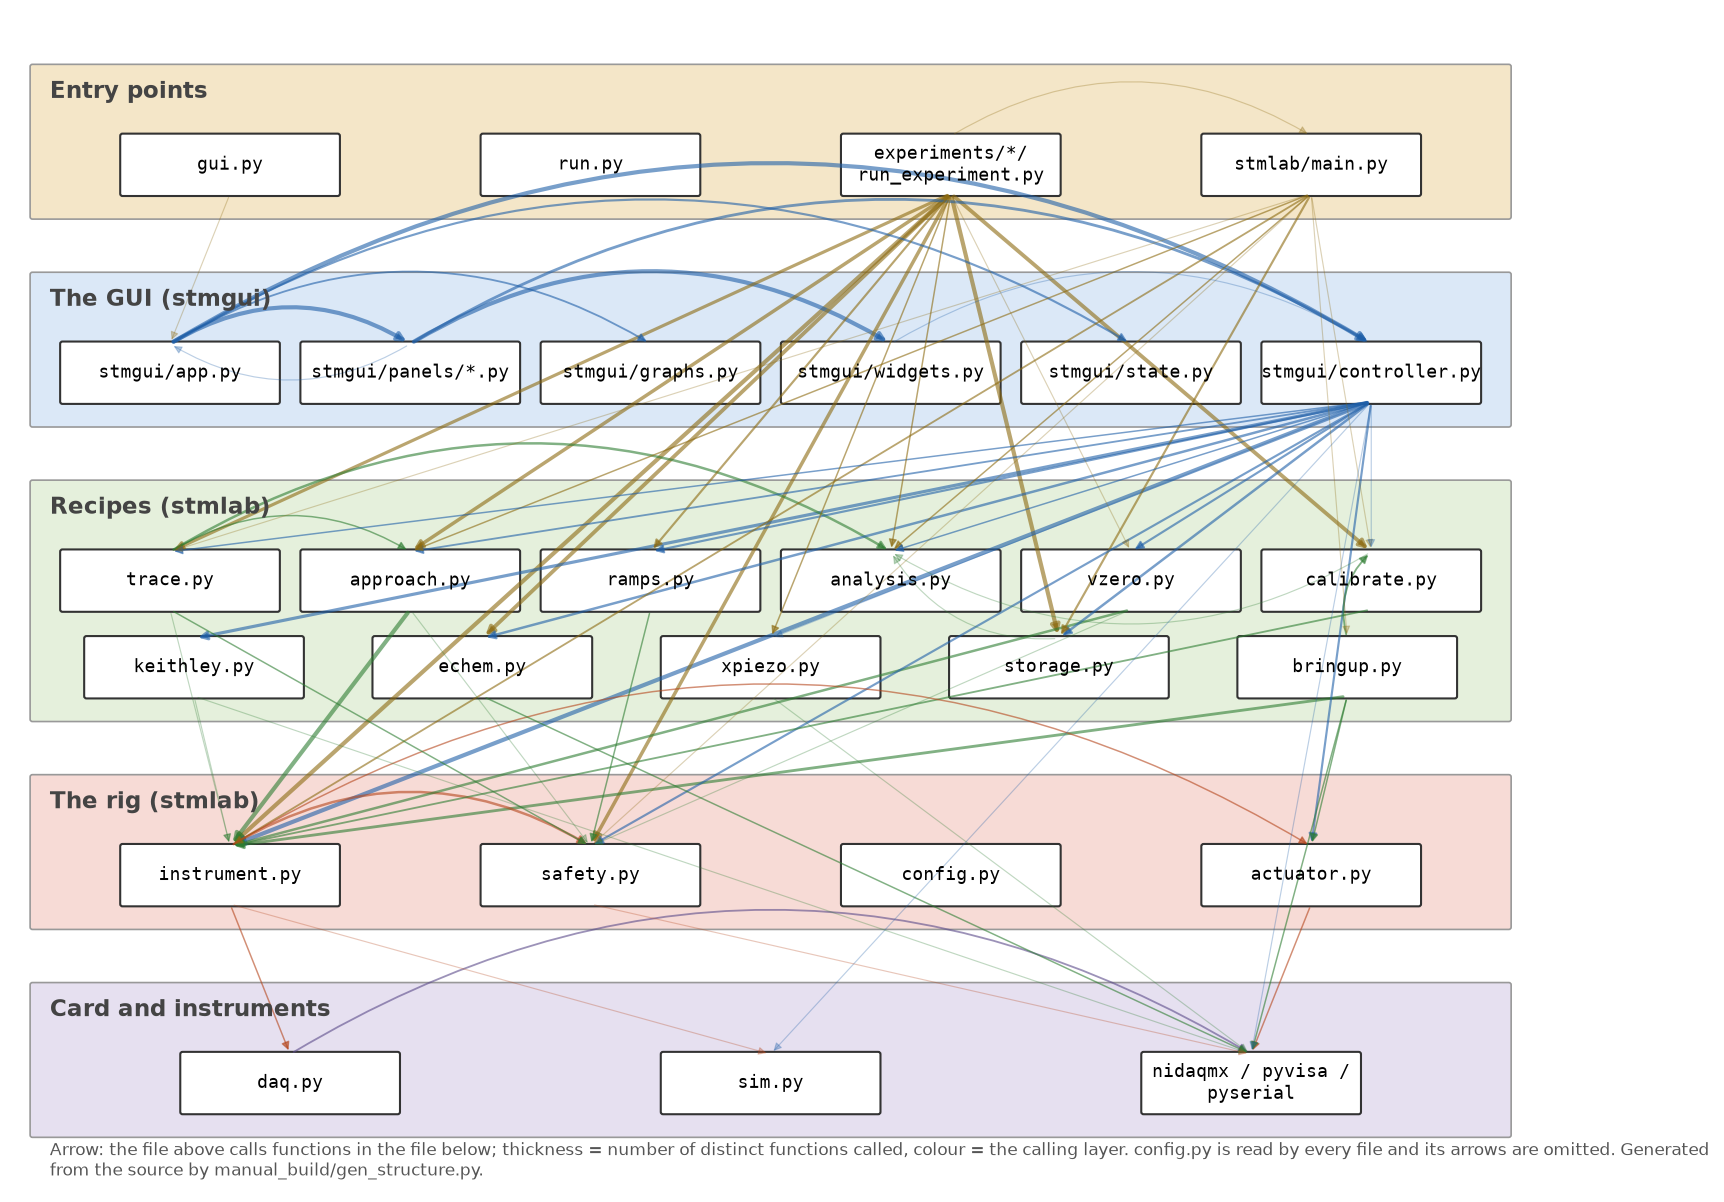
\includegraphics[angle=90,height=0.9\textheight,width=\linewidth,keepaspectratio]{../manual/figures/structure/layers.png}
\\[4pt]{\small The whole code by layer, on its own page. Every arrow is at least one real call found in the source; thickness is the number of distinct functions called, colour is the calling layer. config.py is read by every file and its arrows are left out.}
\end{figure}\clearpage

\small\setlength{\LTleft}{0pt}\setlength{\LTright}{\fill}
\begin{longtable}{@{}>{\raggedright\arraybackslash}p{0.167\linewidth}>{\raggedright\arraybackslash}p{0.335\linewidth}>{\raggedright\arraybackslash}p{0.418\linewidth}@{}}
\toprule
\textbf{Layer} & \textbf{Files} & \textbf{What lives there} \\
\midrule\endhead
Entry points & \texttt{gui.\discretionary{}{}{}py}, \texttt{run.\discretionary{}{}{}py}, \texttt{experiments/\discretionary{}{}{}*/\discretionary{}{}{}run\_\discretionary{}{}{}experiment.\discretionary{}{}{}py}, \texttt{stmlab/\discretionary{}{}{}main.\discretionary{}{}{}py} & Where a run starts. \texttt{gui.\discretionary{}{}{}py} starts the panels; \texttt{run.\discretionary{}{}{}py} forwards to an experiment script or to \texttt{gui.\discretionary{}{}{}py}; \texttt{stmlab/\discretionary{}{}{}main.\discretionary{}{}{}py} is the constant-bias command line that experiment 01 delegates to. \\
The GUI & \texttt{stmgui/\discretionary{}{}{}} & The panels, graphs and menus (Tk thread) and \texttt{controller.\discretionary{}{}{}py} (the worker thread that owns the Rig). Every button is a \texttt{Rig\discretionary{}{}{}Controller} method. \\
Recipes & \texttt{stmlab/\discretionary{}{}{}trace.\discretionary{}{}{}py}, \texttt{approach.\discretionary{}{}{}py}, \texttt{ramps.\discretionary{}{}{}py}, \texttt{analysis.\discretionary{}{}{}py}, \texttt{vzero.\discretionary{}{}{}py}, \texttt{calibrate.\discretionary{}{}{}py}, \texttt{keithley.\discretionary{}{}{}py}, \texttt{echem.\discretionary{}{}{}py}, \texttt{xpiezo.\discretionary{}{}{}py}, \texttt{storage.\discretionary{}{}{}py}, \texttt{bringup.\discretionary{}{}{}py} & The Igor procedures, one concern per file. They know \emph{what} to do to the junction and call the Rig to do it. \\
The rig & \texttt{stmlab/\discretionary{}{}{}instrument.\discretionary{}{}{}py}, \texttt{safety.\discretionary{}{}{}py}, \texttt{config.\discretionary{}{}{}py}, \texttt{actuator.\discretionary{}{}{}py} & \texttt{Rig} is the only way to the card; \texttt{safety} is what it checks; \texttt{config} is every number; \texttt{actuator} is the coarse motor. \\
Card and instruments & \texttt{stmlab/\discretionary{}{}{}daq.\discretionary{}{}{}py}, \texttt{stmlab/\discretionary{}{}{}sim.\discretionary{}{}{}py}, \texttt{nidaqmx}, \texttt{pyvisa}, \texttt{pyserial} & \texttt{Daq\discretionary{}{}{}Session.\discretionary{}{}{}play()} is the one function that talks to the NI card; \texttt{Simulated\discretionary{}{}{}Daq\discretionary{}{}{}Session.\discretionary{}{}{}play()} is its stand-in. \\
\bottomrule
\end{longtable}
\normalsize

\section{Follow one click}

Press \textbf{Find Suppress} on the panel. This is the path, file by file, top to bottom. Every button takes the same route; only the \texttt{\_\discretionary{}{}{}impl} and the recipe module change (chapter 50 lists them all, and the Button map window shows this for any control).

\begin{center}
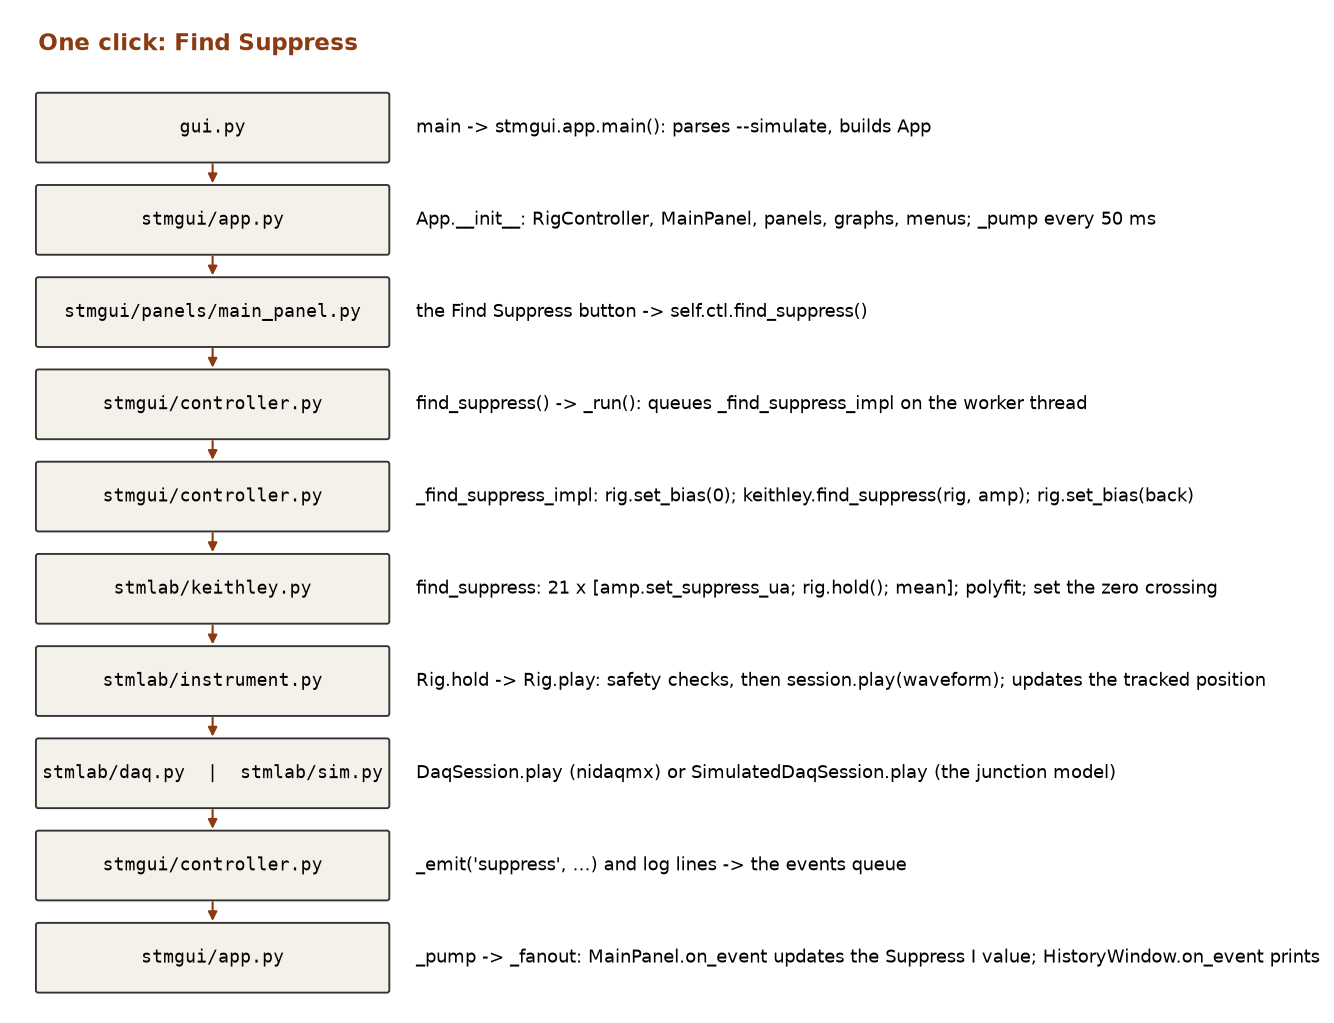
\includegraphics[width=0.9\linewidth]{../manual/figures/structure/click.png}
\\[2pt]{\small One click, from gui.py to the card and back to the screen.}
\end{center}

Three things to notice. The panel never calls \texttt{stmlab} directly: it calls the controller, which queues the work. The controller never draws: it posts events, which \texttt{app.\discretionary{}{}{}py} delivers to the panels 20 times a second. And the recipe (\texttt{keithley.\discretionary{}{}{}find\_\discretionary{}{}{}suppress}) never touches the card: it asks the \texttt{Rig}, which checks the limits and calls \texttt{play()}.

\section{Follow one trace}

\texttt{python run.\discretionary{}{}{}py constant\_\discretionary{}{}{}bias --simulate -n 100}, or Start Measurement in constant mode. The command line path is shown; the GUI's \texttt{\_\discretionary{}{}{}measure\_\discretionary{}{}{}impl} does the same steps in the same order, with its own loop instead of \texttt{trace\_\discretionary{}{}{}loop}.

\begin{center}
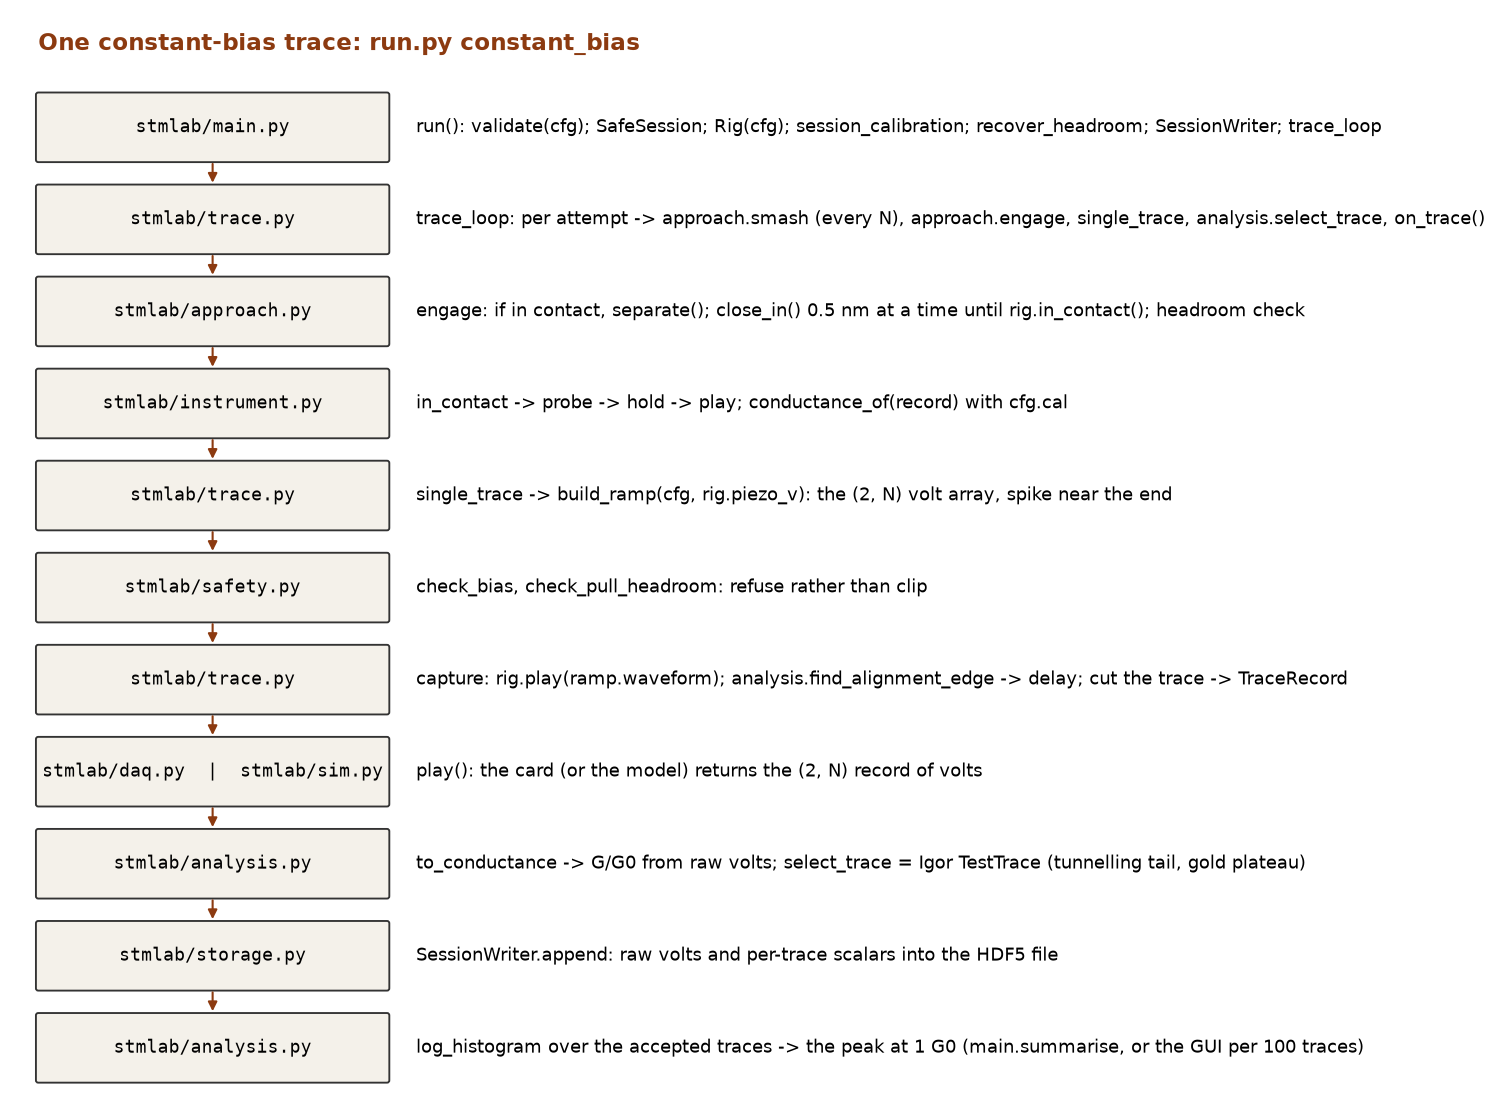
\includegraphics[width=0.9\linewidth]{../manual/figures/structure/trace.png}
\\[2pt]{\small One constant-bias trace, from the command line to the histogram.}
\end{center}

\section{Every file}

\small\setlength{\LTleft}{0pt}\setlength{\LTright}{\fill}
\begin{longtable}{@{}>{\raggedright\arraybackslash}p{0.230\linewidth}>{\raggedright\arraybackslash}p{0.058\linewidth}>{\raggedright\arraybackslash}p{0.403\linewidth}>{\raggedright\arraybackslash}p{0.230\linewidth}@{}}
\toprule
\textbf{File} & \textbf{Lines} & \textbf{Purpose} & \textbf{Called by} \\
\midrule\endhead
\texttt{gui.\discretionary{}{}{}py} & 37 & Launcher for the panels: checks Tk, calls stmgui.app.main & (entry point) \\
\texttt{run.\discretionary{}{}{}py} & 65 & Dispatcher: python run.py <experiment> or gui & (entry point) \\
\texttt{stmlab/\discretionary{}{}{}main.\discretionary{}{}{}py} & 213 & The command line: run / check / summarise / dump-config / bringup & \texttt{experiments/\discretionary{}{}{}01\_\discretionary{}{}{}constant\_\discretionary{}{}{}bias/\discretionary{}{}{}run\_\discretionary{}{}{}experiment.\discretionary{}{}{}py} \\
\texttt{stmlab/\discretionary{}{}{}config.\discretionary{}{}{}py} & 677 & Every number, as dataclasses (RigConfig); validate() refuses unsafe configs & \texttt{experiments/\discretionary{}{}{}* (8 scripts)}, \texttt{stmgui/\discretionary{}{}{}app.\discretionary{}{}{}py}, \texttt{stmgui/\discretionary{}{}{}controller.\discretionary{}{}{}py}, \texttt{stmlab/\discretionary{}{}{}analysis.\discretionary{}{}{}py}, \texttt{stmlab/\discretionary{}{}{}approach.\discretionary{}{}{}py}, \texttt{stmlab/\discretionary{}{}{}bringup.\discretionary{}{}{}py}, \texttt{stmlab/\discretionary{}{}{}calibrate.\discretionary{}{}{}py}, \texttt{stmlab/\discretionary{}{}{}echem.\discretionary{}{}{}py}, \texttt{stmlab/\discretionary{}{}{}instrument.\discretionary{}{}{}py}, \texttt{stmlab/\discretionary{}{}{}main.\discretionary{}{}{}py}, \texttt{stmlab/\discretionary{}{}{}safety.\discretionary{}{}{}py}, \texttt{stmlab/\discretionary{}{}{}storage.\discretionary{}{}{}py}, \texttt{stmlab/\discretionary{}{}{}vzero.\discretionary{}{}{}py} \\
\texttt{stmlab/\discretionary{}{}{}safety.\discretionary{}{}{}py} & 219 & Limits and interlocks: check\_bias, clamp\_piezo, require\_retracted, SafeSession, park\_all\_outputs & \texttt{experiments/\discretionary{}{}{}* (7 scripts)}, \texttt{stmgui/\discretionary{}{}{}controller.\discretionary{}{}{}py}, \texttt{stmlab/\discretionary{}{}{}approach.\discretionary{}{}{}py}, \texttt{stmlab/\discretionary{}{}{}instrument.\discretionary{}{}{}py}, \texttt{stmlab/\discretionary{}{}{}main.\discretionary{}{}{}py}, \texttt{stmlab/\discretionary{}{}{}ramps.\discretionary{}{}{}py}, \texttt{stmlab/\discretionary{}{}{}trace.\discretionary{}{}{}py}, \texttt{stmlab/\discretionary{}{}{}vzero.\discretionary{}{}{}py} \\
\texttt{stmlab/\discretionary{}{}{}instrument.\discretionary{}{}{}py} & 248 & Rig: the one funnel to the card -- play(), hold(), tracked piezo position, coarse\_step() behind the interlock & \texttt{experiments/\discretionary{}{}{}* (7 scripts)}, \texttt{stmgui/\discretionary{}{}{}controller.\discretionary{}{}{}py}, \texttt{stmlab/\discretionary{}{}{}approach.\discretionary{}{}{}py}, \texttt{stmlab/\discretionary{}{}{}bringup.\discretionary{}{}{}py}, \texttt{stmlab/\discretionary{}{}{}calibrate.\discretionary{}{}{}py}, \texttt{stmlab/\discretionary{}{}{}keithley.\discretionary{}{}{}py}, \texttt{stmlab/\discretionary{}{}{}main.\discretionary{}{}{}py}, \texttt{stmlab/\discretionary{}{}{}trace.\discretionary{}{}{}py}, \texttt{stmlab/\discretionary{}{}{}vzero.\discretionary{}{}{}py} \\
\texttt{stmlab/\discretionary{}{}{}daq.\discretionary{}{}{}py} & 229 & The real NI card: DaqSession.play() writes a waveform and reads both inputs & \texttt{stmlab/\discretionary{}{}{}instrument.\discretionary{}{}{}py} \\
\texttt{stmlab/\discretionary{}{}{}sim.\discretionary{}{}{}py} & 214 & The fake card: SimulatedDaqSession with a junction model (gold plateau, molecule, tunnelling) & \texttt{stmgui/\discretionary{}{}{}controller.\discretionary{}{}{}py}, \texttt{stmlab/\discretionary{}{}{}instrument.\discretionary{}{}{}py} \\
\texttt{stmlab/\discretionary{}{}{}actuator.\discretionary{}{}{}py} & 218 & The coarse actuator: NanoPZ over serial, simulated, or none & \texttt{stmgui/\discretionary{}{}{}controller.\discretionary{}{}{}py}, \texttt{stmlab/\discretionary{}{}{}bringup.\discretionary{}{}{}py}, \texttt{stmlab/\discretionary{}{}{}instrument.\discretionary{}{}{}py} \\
\texttt{stmlab/\discretionary{}{}{}approach.\discretionary{}{}{}py} & 188 & engage() = separate + close\_in; smash(); coarse\_approach(); recover\_headroom() & \texttt{experiments/\discretionary{}{}{}* (7 scripts)}, \texttt{stmgui/\discretionary{}{}{}controller.\discretionary{}{}{}py}, \texttt{stmlab/\discretionary{}{}{}main.\discretionary{}{}{}py}, \texttt{stmlab/\discretionary{}{}{}trace.\discretionary{}{}{}py} \\
\texttt{stmlab/\discretionary{}{}{}trace.\discretionary{}{}{}py} & 301 & build\_ramp() the constant pull; capture() play + align at the spike; single\_trace(); trace\_loop() & \texttt{experiments/\discretionary{}{}{}* (7 scripts)}, \texttt{stmgui/\discretionary{}{}{}controller.\discretionary{}{}{}py}, \texttt{stmlab/\discretionary{}{}{}main.\discretionary{}{}{}py} \\
\texttt{stmlab/\discretionary{}{}{}ramps.\discretionary{}{}{}py} & 370 & The four mode waveforms: build\_push\_pull, build\_iv, build\_ac\_hold, build\_hb\_hold & \texttt{experiments/\discretionary{}{}{}* (4 scripts)}, \texttt{stmgui/\discretionary{}{}{}controller.\discretionary{}{}{}py} \\
\texttt{stmlab/\discretionary{}{}{}analysis.\discretionary{}{}{}py} & 363 & Volts to physics: to\_conductance, select\_trace (Igor TestTrace), log\_histogram, peak\_position & \texttt{experiments/\discretionary{}{}{}03\_\discretionary{}{}{}iv\_\discretionary{}{}{}sweep/\discretionary{}{}{}iv\_\discretionary{}{}{}analysis.\discretionary{}{}{}py}, \texttt{stmgui/\discretionary{}{}{}controller.\discretionary{}{}{}py}, \texttt{stmlab/\discretionary{}{}{}calibrate.\discretionary{}{}{}py}, \texttt{stmlab/\discretionary{}{}{}main.\discretionary{}{}{}py}, \texttt{stmlab/\discretionary{}{}{}storage.\discretionary{}{}{}py}, \texttt{stmlab/\discretionary{}{}{}trace.\discretionary{}{}{}py} \\
\texttt{stmlab/\discretionary{}{}{}storage.\discretionary{}{}{}py} & 346 & HDF5 files: SessionWriter / Session, save\_cv\_cycles / CVSession, Igor .ibw readers & \texttt{experiments/\discretionary{}{}{}* (8 scripts)}, \texttt{stmgui/\discretionary{}{}{}controller.\discretionary{}{}{}py}, \texttt{stmlab/\discretionary{}{}{}main.\discretionary{}{}{}py} \\
\texttt{stmlab/\discretionary{}{}{}calibrate.\discretionary{}{}{}py} & 159 & measure\_zero, measure\_group\_delay, session\_calibration & \texttt{experiments/\discretionary{}{}{}* (7 scripts)}, \texttt{stmgui/\discretionary{}{}{}controller.\discretionary{}{}{}py}, \texttt{stmlab/\discretionary{}{}{}bringup.\discretionary{}{}{}py}, \texttt{stmlab/\discretionary{}{}{}main.\discretionary{}{}{}py} \\
\texttt{stmlab/\discretionary{}{}{}keithley.\discretionary{}{}{}py} & 233 & Keithley 428 over GPIB, find\_suppress (Igor TestVirtualGround) & \texttt{stmgui/\discretionary{}{}{}controller.\discretionary{}{}{}py} \\
\texttt{stmlab/\discretionary{}{}{}vzero.\discretionary{}{}{}py} & 149 & measure\_offset (Igor OffsetVoltage) and VzeroTracker (SaveOffset) & \texttt{experiments/\discretionary{}{}{}05\_\discretionary{}{}{}high\_\discretionary{}{}{}bias\_\discretionary{}{}{}hold/\discretionary{}{}{}run\_\discretionary{}{}{}experiment.\discretionary{}{}{}py}, \texttt{stmgui/\discretionary{}{}{}controller.\discretionary{}{}{}py} \\
\texttt{stmlab/\discretionary{}{}{}echem.\discretionary{}{}{}py} & 332 & CounterElectrode gate; CV ramp builders and run\_cv & \texttt{experiments/\discretionary{}{}{}06\_\discretionary{}{}{}echem\_\discretionary{}{}{}gate\_\discretionary{}{}{}cv/\discretionary{}{}{}run\_\discretionary{}{}{}experiment.\discretionary{}{}{}py}, \texttt{stmgui/\discretionary{}{}{}controller.\discretionary{}{}{}py} \\
\texttt{stmlab/\discretionary{}{}{}xpiezo.\discretionary{}{}{}py} & 128 & XPiezo: the lateral piezo on the second card & \texttt{experiments/\discretionary{}{}{}07\_\discretionary{}{}{}lateral\_\discretionary{}{}{}monolayer/\discretionary{}{}{}run\_\discretionary{}{}{}experiment.\discretionary{}{}{}py}, \texttt{stmgui/\discretionary{}{}{}controller.\discretionary{}{}{}py} \\
\texttt{stmlab/\discretionary{}{}{}bringup.\discretionary{}{}{}py} & 464 & Hardware bring-up checks: devices, timing, hold, preamp, actuator & \texttt{stmlab/\discretionary{}{}{}main.\discretionary{}{}{}py} \\
\texttt{stmgui/\discretionary{}{}{}app.\discretionary{}{}{}py} & 324 & App: builds panels, menus, the 50 ms event pump; InitializeExperiment & \texttt{gui.\discretionary{}{}{}py}, \texttt{stmgui/\discretionary{}{}{}panels/\discretionary{}{}{}voltage\_\discretionary{}{}{}offset.\discretionary{}{}{}py} \\
\texttt{stmgui/\discretionary{}{}{}controller.\discretionary{}{}{}py} & 1278 & RigController: every button as a method; one worker thread owns the Rig; events out; COMMAND\_MAP & \texttt{stmgui/\discretionary{}{}{}app.\discretionary{}{}{}py}, \texttt{stmgui/\discretionary{}{}{}panels/\discretionary{}{}{}button\_\discretionary{}{}{}map.\discretionary{}{}{}py}, \texttt{stmgui/\discretionary{}{}{}panels/\discretionary{}{}{}echem\_\discretionary{}{}{}panel.\discretionary{}{}{}py}, \texttt{stmgui/\discretionary{}{}{}panels/\discretionary{}{}{}main\_\discretionary{}{}{}panel.\discretionary{}{}{}py}, \texttt{stmgui/\discretionary{}{}{}widgets.\discretionary{}{}{}py} \\
\texttt{stmgui/\discretionary{}{}{}state.\discretionary{}{}{}py} & 337 & GuiOptions (Igor globals without a config home), Param, PARAMS binding table & \texttt{stmgui/\discretionary{}{}{}app.\discretionary{}{}{}py} \\
\texttt{stmgui/\discretionary{}{}{}widgets.\discretionary{}{}{}py} & 331 & SetVariable, ValDisplay, CheckBox, button, Tooltip, Inspector binding & \texttt{stmgui/\discretionary{}{}{}panels/\discretionary{}{}{}echem\_\discretionary{}{}{}panel.\discretionary{}{}{}py}, \texttt{stmgui/\discretionary{}{}{}panels/\discretionary{}{}{}main\_\discretionary{}{}{}panel.\discretionary{}{}{}py}, \texttt{stmgui/\discretionary{}{}{}panels/\discretionary{}{}{}voltage\_\discretionary{}{}{}offset.\discretionary{}{}{}py} \\
\texttt{stmgui/\discretionary{}{}{}graphs.\discretionary{}{}{}py} & 388 & The nine Igor graph windows (matplotlib in Tk) and GraphSet routing & \texttt{stmgui/\discretionary{}{}{}app.\discretionary{}{}{}py} \\
\texttt{stmgui/\discretionary{}{}{}panels/\discretionary{}{}{}main\_\discretionary{}{}{}panel.\discretionary{}{}{}py} & 470 & The BreakJunctionMeasurement panel & \texttt{stmgui/\discretionary{}{}{}app.\discretionary{}{}{}py} \\
\texttt{stmgui/\discretionary{}{}{}panels/\discretionary{}{}{}voltage\_\discretionary{}{}{}offset.\discretionary{}{}{}py} & 90 & The Voltage\_Offset panel & \texttt{stmgui/\discretionary{}{}{}app.\discretionary{}{}{}py} \\
\texttt{stmgui/\discretionary{}{}{}panels/\discretionary{}{}{}echem\_\discretionary{}{}{}panel.\discretionary{}{}{}py} & 103 & The EChem panel & \texttt{stmgui/\discretionary{}{}{}app.\discretionary{}{}{}py} \\
\texttt{stmgui/\discretionary{}{}{}panels/\discretionary{}{}{}history.\discretionary{}{}{}py} & 53 & The History window & \texttt{stmgui/\discretionary{}{}{}app.\discretionary{}{}{}py} \\
\texttt{stmgui/\discretionary{}{}{}panels/\discretionary{}{}{}button\_\discretionary{}{}{}map.\discretionary{}{}{}py} & 110 & The Button map and Inspector windows & \texttt{stmgui/\discretionary{}{}{}app.\discretionary{}{}{}py} \\
\texttt{experiments/\discretionary{}{}{}01\_\discretionary{}{}{}constant\_\discretionary{}{}{}bias/\discretionary{}{}{}run\_\discretionary{}{}{}experiment.\discretionary{}{}{}py} & 47 & delegates to stmlab.main (the reference loop) & \texttt{run.\discretionary{}{}{}py} \\
\texttt{experiments/\discretionary{}{}{}02\_\discretionary{}{}{}push\_\discretionary{}{}{}pull/\discretionary{}{}{}run\_\discretionary{}{}{}experiment.\discretionary{}{}{}py} & 231 & loop: engage, ramps.build\_push\_pull, capture, save & \texttt{run.\discretionary{}{}{}py} \\
\texttt{experiments/\discretionary{}{}{}03\_\discretionary{}{}{}iv\_\discretionary{}{}{}sweep/\discretionary{}{}{}run\_\discretionary{}{}{}experiment.\discretionary{}{}{}py} & 312 & loop: engage, ramps.build\_iv, capture, save; iv\_analysis.py reads it back & \texttt{run.\discretionary{}{}{}py} \\
\texttt{experiments/\discretionary{}{}{}04\_\discretionary{}{}{}ac\_\discretionary{}{}{}hold/\discretionary{}{}{}run\_\discretionary{}{}{}experiment.\discretionary{}{}{}py} & 287 & loop: engage, ramps.build\_ac\_hold, capture, save & \texttt{run.\discretionary{}{}{}py} \\
\texttt{experiments/\discretionary{}{}{}05\_\discretionary{}{}{}high\_\discretionary{}{}{}bias\_\discretionary{}{}{}hold/\discretionary{}{}{}run\_\discretionary{}{}{}experiment.\discretionary{}{}{}py} & 281 & loop: engage, ramps.build\_hb\_hold (optionally at Vzero), capture, save & \texttt{run.\discretionary{}{}{}py} \\
\texttt{experiments/\discretionary{}{}{}06\_\discretionary{}{}{}echem\_\discretionary{}{}{}gate\_\discretionary{}{}{}cv/\discretionary{}{}{}run\_\discretionary{}{}{}experiment.\discretionary{}{}{}py} & 332 & gate / cv / traces sub-commands over echem.py & \texttt{run.\discretionary{}{}{}py} \\
\texttt{experiments/\discretionary{}{}{}07\_\discretionary{}{}{}lateral\_\discretionary{}{}{}monolayer/\discretionary{}{}{}run\_\discretionary{}{}{}experiment.\discretionary{}{}{}py} & 244 & per site: trace\_loop, withdraw, xpiezo.move\_nm, approach & \texttt{run.\discretionary{}{}{}py} \\
\texttt{experiments/\discretionary{}{}{}08\_\discretionary{}{}{}bias\_\discretionary{}{}{}series/\discretionary{}{}{}run\_\discretionary{}{}{}experiment.\discretionary{}{}{}py} & 318 & Igor rungo: one trace\_loop per bias, resumable & \texttt{run.\discretionary{}{}{}py} \\
\bottomrule
\end{longtable}
\normalsize

\section{Who calls whom, file by file}

For each file: the functions it defines, and for each one the functions in \emph{other} files it calls (\texttt{file: function}). Calls within the same file are left out, as are calls to numpy, h5py, Tk and the standard library. A method is shown as \texttt{Class.\discretionary{}{}{}method}; \texttt{self.\discretionary{}{}{}x} means a method of the same class.

\subsection{gui.py}

\small\setlength{\LTleft}{0pt}\setlength{\LTright}{\fill}
\begin{longtable}{@{}>{\raggedright\arraybackslash}p{0.280\linewidth}>{\raggedright\arraybackslash}p{0.640\linewidth}@{}}
\toprule
\textbf{Function} & \textbf{Calls (file: function)} \\
\midrule\endhead
\texttt{(module level)} & stmgui/app.py: main \\
\bottomrule
\end{longtable}
\normalsize

\subsection{run.py}

Calls nothing in another file of this package (a leaf: it is called, it does not call).

\subsection{stmlab/main.py}

\small\setlength{\LTleft}{0pt}\setlength{\LTright}{\fill}
\begin{longtable}{@{}>{\raggedright\arraybackslash}p{0.280\linewidth}>{\raggedright\arraybackslash}p{0.640\linewidth}@{}}
\toprule
\textbf{Function} & \textbf{Calls (file: function)} \\
\midrule\endhead
\texttt{run (:25)} & stmlab/approach.py: coarse\_approach; stmlab/approach.py: recover\_headroom; stmlab/calibrate.py: session\_calibration; stmlab/config.py: validate; stmlab/instrument.py: Rig; stmlab/instrument.py: Rig.set\_bias; stmlab/instrument.py: Rig.withdraw; stmlab/safety.py: SafeSession; stmlab/storage.py: SessionWriter; stmlab/storage.py: SessionWriter.write\_summary; stmlab/trace.py: trace\_loop \\
\texttt{summarise (:74)} & stmlab/analysis.py: log\_histogram; stmlab/analysis.py: peak\_position; stmlab/storage.py: Session; stmlab/storage.py: Session.conductances \\
\texttt{main (:149)} & stmlab/bringup.py: main; stmlab/config.py: RigConfig; stmlab/config.py: RigConfig.from\_json; stmlab/config.py: RigConfig.to\_json; stmlab/config.py: validate \\
\bottomrule
\end{longtable}
\normalsize

\subsection{stmlab/config.py}

Calls nothing in another file of this package (a leaf: it is called, it does not call).

\subsection{stmlab/safety.py}

\small\setlength{\LTleft}{0pt}\setlength{\LTright}{\fill}
\begin{longtable}{@{}>{\raggedright\arraybackslash}p{0.280\linewidth}>{\raggedright\arraybackslash}p{0.640\linewidth}@{}}
\toprule
\textbf{Function} & \textbf{Calls (file: function)} \\
\midrule\endhead
\texttt{check\_\discretionary{}{}{}pull\_\discretionary{}{}{}headroom (:72)} & stmlab/config.py: Calibration.nm\_to\_piezo\_volts \\
\texttt{park\_\discretionary{}{}{}all\_\discretionary{}{}{}outputs (:163)} & stmlab/config.py: ChannelMap.path \\
\bottomrule
\end{longtable}
\normalsize

\subsection{stmlab/instrument.py}

\small\setlength{\LTleft}{0pt}\setlength{\LTright}{\fill}
\begin{longtable}{@{}>{\raggedright\arraybackslash}p{0.280\linewidth}>{\raggedright\arraybackslash}p{0.640\linewidth}@{}}
\toprule
\textbf{Function} & \textbf{Calls (file: function)} \\
\midrule\endhead
\texttt{Rig.\discretionary{}{}{}open (:41)} & stmlab/actuator.py: make\_actuator; stmlab/daq.py: DaqSession; stmlab/sim.py: SimulatedDaqSession \\
\texttt{Rig.\discretionary{}{}{}piezo\_\discretionary{}{}{}nm (:90)} & stmlab/config.py: Calibration.piezo\_volts\_to\_nm \\
\texttt{Rig.\discretionary{}{}{}play (:104)} & stmlab/daq.py: DaqSession.play \\
\texttt{Rig.\discretionary{}{}{}hold (:130)} & stmlab/safety.py: check\_bias; stmlab/safety.py: clamp\_piezo \\
\texttt{Rig.\discretionary{}{}{}piezo\_\discretionary{}{}{}step\_\discretionary{}{}{}nm (:152)} & stmlab/config.py: Calibration.nm\_to\_piezo\_volts \\
\texttt{Rig.\discretionary{}{}{}set\_\discretionary{}{}{}bias (:157)} & stmlab/safety.py: check\_bias \\
\texttt{Rig.\discretionary{}{}{}conductance\_\discretionary{}{}{}of (:189)} & stmlab/config.py: Calibration.volts\_to\_amps \\
\texttt{Rig.\discretionary{}{}{}read\_\discretionary{}{}{}current\_\discretionary{}{}{}ua (:203)} & stmlab/config.py: Calibration.volts\_to\_amps \\
\texttt{Rig.\discretionary{}{}{}coarse\_\discretionary{}{}{}step (:229)} & stmlab/actuator.py: Actuator.step; stmlab/safety.py: check\_step\_budget; stmlab/safety.py: require\_retracted \\
\bottomrule
\end{longtable}
\normalsize

\subsection{stmlab/daq.py}

Calls nothing in another file of this package (a leaf: it is called, it does not call).

\subsection{stmlab/sim.py}

Calls nothing in another file of this package (a leaf: it is called, it does not call).

\subsection{stmlab/actuator.py}

Calls nothing in another file of this package (a leaf: it is called, it does not call).

\subsection{stmlab/approach.py}

\small\setlength{\LTleft}{0pt}\setlength{\LTright}{\fill}
\begin{longtable}{@{}>{\raggedright\arraybackslash}p{0.280\linewidth}>{\raggedright\arraybackslash}p{0.640\linewidth}@{}}
\toprule
\textbf{Function} & \textbf{Calls (file: function)} \\
\midrule\endhead
\texttt{\_\discretionary{}{}{}headroom\_\discretionary{}{}{}ok (:29)} & stmlab/config.py: Calibration.nm\_to\_piezo\_volts \\
\texttt{separate (:35)} & stmlab/instrument.py: Rig.piezo\_step\_nm; stmlab/instrument.py: Rig.probe \\
\texttt{close\_\discretionary{}{}{}in (:55)} & stmlab/instrument.py: Rig.in\_contact; stmlab/instrument.py: Rig.piezo\_step\_nm \\
\texttt{engage (:71)} & stmlab/instrument.py: Rig.in\_contact \\
\texttt{smash (:102)} & stmlab/instrument.py: Rig.piezo\_step\_nm \\
\texttt{coarse\_\discretionary{}{}{}approach (:120)} & stmlab/instrument.py: Rig.coarse\_step; stmlab/instrument.py: Rig.read\_current\_ua; stmlab/safety.py: require\_retracted \\
\texttt{withdraw\_\discretionary{}{}{}coarse (:161)} & stmlab/instrument.py: Rig.coarse\_step \\
\texttt{recover\_\discretionary{}{}{}headroom (:167)} & stmlab/instrument.py: Rig.withdraw \\
\bottomrule
\end{longtable}
\normalsize

\subsection{stmlab/trace.py}

\small\setlength{\LTleft}{0pt}\setlength{\LTright}{\fill}
\begin{longtable}{@{}>{\raggedright\arraybackslash}p{0.280\linewidth}>{\raggedright\arraybackslash}p{0.640\linewidth}@{}}
\toprule
\textbf{Function} & \textbf{Calls (file: function)} \\
\midrule\endhead
\texttt{Trace\discretionary{}{}{}Record.\discretionary{}{}{}conductance\_\discretionary{}{}{}g0 (:60)} & stmlab/analysis.py: to\_conductance \\
\texttt{Trace\discretionary{}{}{}Record.\discretionary{}{}{}displacement\_\discretionary{}{}{}nm (:68)} & stmlab/analysis.py: displacement\_nm \\
\texttt{build\_\discretionary{}{}{}ramp (:77)} & stmlab/analysis.py: spike\_indices; stmlab/safety.py: check\_bias; stmlab/safety.py: check\_pull\_headroom \\
\texttt{capture (:166)} & stmlab/instrument.py: Rig.play \\
\texttt{\_\discretionary{}{}{}measure\_\discretionary{}{}{}delay (:206)} & stmlab/analysis.py: find\_alignment\_edge \\
\texttt{trace\_\discretionary{}{}{}loop (:236)} & stmlab/analysis.py: select\_trace; stmlab/approach.py: engage; stmlab/approach.py: smash \\
\bottomrule
\end{longtable}
\normalsize

\subsection{stmlab/ramps.py}

\small\setlength{\LTleft}{0pt}\setlength{\LTright}{\fill}
\begin{longtable}{@{}>{\raggedright\arraybackslash}p{0.280\linewidth}>{\raggedright\arraybackslash}p{0.640\linewidth}@{}}
\toprule
\textbf{Function} & \textbf{Calls (file: function)} \\
\midrule\endhead
\texttt{\_\discretionary{}{}{}assemble (:90)} & stmlab/safety.py: SafetyViolation; stmlab/safety.py: check\_bias \\
\bottomrule
\end{longtable}
\normalsize

\subsection{stmlab/analysis.py}

\small\setlength{\LTleft}{0pt}\setlength{\LTright}{\fill}
\begin{longtable}{@{}>{\raggedright\arraybackslash}p{0.280\linewidth}>{\raggedright\arraybackslash}p{0.640\linewidth}@{}}
\toprule
\textbf{Function} & \textbf{Calls (file: function)} \\
\midrule\endhead
\texttt{to\_\discretionary{}{}{}conductance (:66)} & stmlab/config.py: Calibration.volts\_to\_amps \\
\bottomrule
\end{longtable}
\normalsize

\subsection{stmlab/storage.py}

\small\setlength{\LTleft}{0pt}\setlength{\LTright}{\fill}
\begin{longtable}{@{}>{\raggedright\arraybackslash}p{0.280\linewidth}>{\raggedright\arraybackslash}p{0.640\linewidth}@{}}
\toprule
\textbf{Function} & \textbf{Calls (file: function)} \\
\midrule\endhead
\texttt{Session\discretionary{}{}{}Writer.\discretionary{}{}{}open (:50)} & stmlab/config.py: RigConfig.to\_dict \\
\texttt{Session.\discretionary{}{}{}\_\discretionary{}{}{}\_\discretionary{}{}{}init\_\discretionary{}{}{}\_\discretionary{}{}{} (:160)} & stmlab/config.py: RigConfig.from\_dict \\
\texttt{Session.\discretionary{}{}{}conductance (:183)} & stmlab/analysis.py: to\_conductance \\
\texttt{save\_\discretionary{}{}{}cv\_\discretionary{}{}{}cycles (:255)} & stmlab/config.py: RigConfig.to\_dict \\
\texttt{CVSession.\discretionary{}{}{}\_\discretionary{}{}{}\_\discretionary{}{}{}init\_\discretionary{}{}{}\_\discretionary{}{}{} (:305)} & stmlab/config.py: RigConfig.from\_dict \\
\texttt{CVSession.\discretionary{}{}{}current\_\discretionary{}{}{}a (:338)} & stmlab/config.py: Calibration.volts\_to\_amps \\
\bottomrule
\end{longtable}
\normalsize

\subsection{stmlab/calibrate.py}

\small\setlength{\LTleft}{0pt}\setlength{\LTright}{\fill}
\begin{longtable}{@{}>{\raggedright\arraybackslash}p{0.280\linewidth}>{\raggedright\arraybackslash}p{0.640\linewidth}@{}}
\toprule
\textbf{Function} & \textbf{Calls (file: function)} \\
\midrule\endhead
\texttt{measure\_\discretionary{}{}{}zero (:28)} & stmlab/config.py: Calibration.volts\_to\_amps; stmlab/instrument.py: Rig.hold \\
\texttt{measure\_\discretionary{}{}{}group\_\discretionary{}{}{}delay (:57)} & stmlab/analysis.py: find\_alignment\_edge; stmlab/instrument.py: Rig.play \\
\texttt{measure\_\discretionary{}{}{}gain\_\discretionary{}{}{}offset (:105)} & stmlab/instrument.py: Rig.hold \\
\bottomrule
\end{longtable}
\normalsize

\subsection{stmlab/keithley.py}

\small\setlength{\LTleft}{0pt}\setlength{\LTright}{\fill}
\begin{longtable}{@{}>{\raggedright\arraybackslash}p{0.280\linewidth}>{\raggedright\arraybackslash}p{0.640\linewidth}@{}}
\toprule
\textbf{Function} & \textbf{Calls (file: function)} \\
\midrule\endhead
\texttt{find\_\discretionary{}{}{}suppress (:199)} & stmlab/instrument.py: Rig.hold \\
\bottomrule
\end{longtable}
\normalsize

\subsection{stmlab/vzero.py}

\small\setlength{\LTleft}{0pt}\setlength{\LTright}{\fill}
\begin{longtable}{@{}>{\raggedright\arraybackslash}p{0.280\linewidth}>{\raggedright\arraybackslash}p{0.640\linewidth}@{}}
\toprule
\textbf{Function} & \textbf{Calls (file: function)} \\
\midrule\endhead
\texttt{\_\discretionary{}{}{}ensure\_\discretionary{}{}{}contact (:49)} & stmlab/instrument.py: Rig.in\_contact; stmlab/instrument.py: Rig.piezo\_step\_nm; stmlab/instrument.py: Rig.set\_bias; stmlab/safety.py: SafetyViolation \\
\texttt{measure\_\discretionary{}{}{}offset (:66)} & stmlab/config.py: Calibration.volts\_to\_amps; stmlab/instrument.py: Rig.hold; stmlab/instrument.py: Rig.set\_bias \\
\bottomrule
\end{longtable}
\normalsize

\subsection{stmlab/echem.py}

\small\setlength{\LTleft}{0pt}\setlength{\LTright}{\fill}
\begin{longtable}{@{}>{\raggedright\arraybackslash}p{0.280\linewidth}>{\raggedright\arraybackslash}p{0.640\linewidth}@{}}
\toprule
\textbf{Function} & \textbf{Calls (file: function)} \\
\midrule\endhead
\texttt{\_\discretionary{}{}{}run\_\discretionary{}{}{}cv\_\discretionary{}{}{}hardware (:283)} & stmlab/config.py: ChannelMap.path \\
\bottomrule
\end{longtable}
\normalsize

\subsection{stmlab/xpiezo.py}

Calls nothing in another file of this package (a leaf: it is called, it does not call).

\subsection{stmlab/bringup.py}

\small\setlength{\LTleft}{0pt}\setlength{\LTright}{\fill}
\begin{longtable}{@{}>{\raggedright\arraybackslash}p{0.280\linewidth}>{\raggedright\arraybackslash}p{0.640\linewidth}@{}}
\toprule
\textbf{Function} & \textbf{Calls (file: function)} \\
\midrule\endhead
\texttt{step\_\discretionary{}{}{}devices (:68)} & stmlab/config.py: ChannelMap.path \\
\texttt{step\_\discretionary{}{}{}timing (:143)} & stmlab/calibrate.py: measure\_group\_delay; stmlab/instrument.py: Rig \\
\texttt{step\_\discretionary{}{}{}hold (:191)} & stmlab/instrument.py: Rig; stmlab/instrument.py: Rig.hold; stmlab/instrument.py: Rig.piezo\_goto \\
\texttt{step\_\discretionary{}{}{}preamp (:250)} & stmlab/calibrate.py: expected\_resistor\_v; stmlab/calibrate.py: measure\_zero; stmlab/config.py: Calibration.volts\_to\_amps; stmlab/instrument.py: Rig; stmlab/instrument.py: Rig.hold \\
\texttt{step\_\discretionary{}{}{}actuator (:309)} & stmlab/actuator.py: NanoPZActuator; stmlab/actuator.py: list\_serial\_ports \\
\texttt{main (:410)} & stmlab/config.py: RigConfig; stmlab/config.py: RigConfig.from\_json \\
\bottomrule
\end{longtable}
\normalsize

\subsection{stmgui/app.py}

\small\setlength{\LTleft}{0pt}\setlength{\LTright}{\fill}
\begin{longtable}{@{}>{\raggedright\arraybackslash}p{0.280\linewidth}>{\raggedright\arraybackslash}p{0.640\linewidth}@{}}
\toprule
\textbf{Function} & \textbf{Calls (file: function)} \\
\midrule\endhead
\texttt{App.\discretionary{}{}{}\_\discretionary{}{}{}\_\discretionary{}{}{}init\_\discretionary{}{}{}\_\discretionary{}{}{} (:41)} & stmgui/controller.py: RigController; stmgui/controller.py: RigController.connect\_instruments; stmgui/controller.py: RigController.request\_stop; stmgui/graphs.py: GraphSet; stmgui/panels/echem\_panel.py: EChemPanel; stmgui/panels/history.py: HistoryWindow; stmgui/panels/main\_panel.py: MainPanel; stmgui/panels/voltage\_offset.py: VoltageOffsetPanel; stmgui/state.py: GuiState; stmgui/state.py: simulated\_state \\
\texttt{App.\discretionary{}{}{}log (:95)} & stmgui/panels/history.py: HistoryWindow.append \\
\texttt{App.\discretionary{}{}{}\_\discretionary{}{}{}build\_\discretionary{}{}{}menus (:98)} & stmgui/graphs.py: GraphSet.names; stmgui/graphs.py: GraphSet.show \\
\texttt{App.\discretionary{}{}{}\_\discretionary{}{}{}load\_\discretionary{}{}{}cfg (:156)} & stmgui/controller.py: RigController.load\_config \\
\texttt{App.\discretionary{}{}{}\_\discretionary{}{}{}save\_\discretionary{}{}{}cfg (:166)} & stmgui/controller.py: RigController.save\_config \\
\texttt{App.\discretionary{}{}{}\_\discretionary{}{}{}open\_\discretionary{}{}{}data (:173)} & stmgui/controller.py: RigController.data\_dir \\
\texttt{App.\discretionary{}{}{}\_\discretionary{}{}{}rungo (:184)} & stmgui/controller.py: RigController.rungo \\
\texttt{App.\discretionary{}{}{}\_\discretionary{}{}{}lateral (:204)} & stmgui/controller.py: RigController.lateral\_expt \\
\texttt{App.\discretionary{}{}{}\_\discretionary{}{}{}move\_\discretionary{}{}{}x (:221)} & stmgui/controller.py: RigController.move\_xpiezo \\
\texttt{App.\discretionary{}{}{}show\_\discretionary{}{}{}button\_\discretionary{}{}{}map (:227)} & stmgui/panels/button\_map.py: ButtonMapWindow; stmgui/panels/button\_map.py: ButtonMapWindow.refresh; stmgui/panels/button\_map.py: ButtonMapWindow.show \\
\texttt{App.\discretionary{}{}{}inspect (:237)} & stmgui/panels/button\_map.py: InspectorWindow; stmgui/panels/button\_map.py: InspectorWindow.show\_text; stmgui/panels/history.py: HistoryWindow.append \\
\texttt{App.\discretionary{}{}{}\_\discretionary{}{}{}fanout (:258)} & stmgui/panels/history.py: HistoryWindow.append \\
\texttt{App.\discretionary{}{}{}quit (:287)} & stmgui/controller.py: RigController.shutdown \\
\texttt{main (:299)} & stmgui/state.py: GuiState; stmgui/state.py: simulated\_state; stmlab/config.py: RigConfig.from\_json \\
\bottomrule
\end{longtable}
\normalsize

\subsection{stmgui/controller.py}

\small\setlength{\LTleft}{0pt}\setlength{\LTright}{\fill}
\begin{longtable}{@{}>{\raggedright\arraybackslash}p{0.280\linewidth}>{\raggedright\arraybackslash}p{0.640\linewidth}@{}}
\toprule
\textbf{Function} & \textbf{Calls (file: function)} \\
\midrule\endhead
\texttt{Rig\discretionary{}{}{}Controller.\discretionary{}{}{}\_\discretionary{}{}{}\_\discretionary{}{}{}init\_\discretionary{}{}{}\_\discretionary{}{}{} (:93)} & stmlab/vzero.py: VzeroTracker \\
\texttt{Rig\discretionary{}{}{}Controller.\discretionary{}{}{}shutdown (:204)} & stmlab/keithley.py: Keithley428.close \\
\texttt{Rig\discretionary{}{}{}Controller.\discretionary{}{}{}\_\discretionary{}{}{}connect\_\discretionary{}{}{}impl (:269)} & stmlab/keithley.py: make\_keithley \\
\texttt{Rig\discretionary{}{}{}Controller.\discretionary{}{}{}\_\discretionary{}{}{}make\_\discretionary{}{}{}rig (:292)} & stmlab/actuator.py: SimulatedActuator; stmlab/instrument.py: Rig; stmlab/safety.py: park\_all\_outputs; stmlab/safety.py: verify\_devices; stmlab/sim.py: SimulatedDaqSession \\
\texttt{Rig\discretionary{}{}{}Controller.\discretionary{}{}{}\_\discretionary{}{}{}start\_\discretionary{}{}{}writing\_\discretionary{}{}{}impl (:305)} & stmlab/calibrate.py: session\_calibration; stmlab/config.py: Calibration.nm\_to\_piezo\_volts; stmlab/config.py: validate; stmlab/instrument.py: Rig.hold \\
\texttt{Rig\discretionary{}{}{}Controller.\discretionary{}{}{}\_\discretionary{}{}{}kill\_\discretionary{}{}{}tasks\_\discretionary{}{}{}impl (:333)} & stmlab/instrument.py: Rig.close; stmlab/keithley.py: Keithley428.zero\_check \\
\texttt{Rig\discretionary{}{}{}Controller.\discretionary{}{}{}\_\discretionary{}{}{}reset\_\discretionary{}{}{}daq\_\discretionary{}{}{}impl (:366)} & stmlab/echem.py: CounterElectrode.off; stmlab/safety.py: park\_all\_outputs \\
\texttt{Rig\discretionary{}{}{}Controller.\discretionary{}{}{}\_\discretionary{}{}{}background\_\discretionary{}{}{}read (:399)} & stmlab/config.py: Calibration.volts\_to\_amps; stmlab/instrument.py: Rig.hold \\
\texttt{Rig\discretionary{}{}{}Controller.\discretionary{}{}{}\_\discretionary{}{}{}piezo\_\discretionary{}{}{}step\_\discretionary{}{}{}impl (:434)} & stmlab/instrument.py: Rig.piezo\_step\_nm \\
\texttt{Rig\discretionary{}{}{}Controller.\discretionary{}{}{}\_\discretionary{}{}{}piezo\_\discretionary{}{}{}goto\_\discretionary{}{}{}impl (:445)} & stmlab/instrument.py: Rig.piezo\_goto \\
\texttt{Rig\discretionary{}{}{}Controller.\discretionary{}{}{}\_\discretionary{}{}{}set\_\discretionary{}{}{}tip\_\discretionary{}{}{}bias\_\discretionary{}{}{}impl (:460)} & stmlab/instrument.py: Rig.set\_bias; stmlab/keithley.py: Keithley428.set\_bias\_mv; stmlab/safety.py: SafetyViolation \\
\texttt{Rig\discretionary{}{}{}Controller.\discretionary{}{}{}\_\discretionary{}{}{}set\_\discretionary{}{}{}gain\_\discretionary{}{}{}impl (:483)} & stmlab/keithley.py: Keithley428.set\_gain \\
\texttt{Rig\discretionary{}{}{}Controller.\discretionary{}{}{}\_\discretionary{}{}{}find\_\discretionary{}{}{}suppress\_\discretionary{}{}{}impl (:532)} & stmlab/instrument.py: Rig.set\_bias; stmlab/keithley.py: find\_suppress \\
\texttt{Rig\discretionary{}{}{}Controller.\discretionary{}{}{}\_\discretionary{}{}{}find\_\discretionary{}{}{}offset\_\discretionary{}{}{}impl (:556)} & stmlab/vzero.py: measure\_offset \\
\texttt{Rig\discretionary{}{}{}Controller.\discretionary{}{}{}\_\discretionary{}{}{}step\_\discretionary{}{}{}actuator\_\discretionary{}{}{}impl (:586)} & stmlab/actuator.py: Actuator.close; stmlab/actuator.py: Actuator.step; stmlab/actuator.py: make\_actuator; stmlab/instrument.py: Rig.coarse\_step \\
\texttt{Rig\discretionary{}{}{}Controller.\discretionary{}{}{}\_\discretionary{}{}{}approach\_\discretionary{}{}{}impl (:605)} & stmlab/approach.py: ApproachError; stmlab/config.py: Calibration.volts\_to\_amps; stmlab/instrument.py: Rig.coarse\_step; stmlab/instrument.py: Rig.hold \\
\texttt{Rig\discretionary{}{}{}Controller.\discretionary{}{}{}\_\discretionary{}{}{}build\_\discretionary{}{}{}ramp (:681)} & stmlab/ramps.py: build\_ac\_hold; stmlab/ramps.py: build\_hb\_hold; stmlab/ramps.py: build\_iv; stmlab/ramps.py: build\_push\_pull; stmlab/trace.py: build\_ramp \\
\texttt{Rig\discretionary{}{}{}Controller.\discretionary{}{}{}\_\discretionary{}{}{}open\_\discretionary{}{}{}writer (:699)} & stmlab/storage.py: SessionWriter \\
\texttt{Rig\discretionary{}{}{}Controller.\discretionary{}{}{}\_\discretionary{}{}{}close\_\discretionary{}{}{}writer (:707)} & stmlab/storage.py: SessionWriter.close; stmlab/storage.py: SessionWriter.write\_summary; stmlab/vzero.py: VzeroTracker.as\_arrays \\
\texttt{Rig\discretionary{}{}{}Controller.\discretionary{}{}{}\_\discretionary{}{}{}measure\_\discretionary{}{}{}impl (:722)} & stmlab/analysis.py: select\_trace; stmlab/approach.py: recover\_headroom; stmlab/approach.py: smash; stmlab/config.py: Calibration.piezo\_volts\_to\_nm; stmlab/config.py: validate; stmlab/instrument.py: Rig.set\_bias; stmlab/storage.py: SessionWriter.append; stmlab/trace.py: capture; stmlab/vzero.py: VzeroTracker.maybe\_measure \\
\texttt{Rig\discretionary{}{}{}Controller.\discretionary{}{}{}\_\discretionary{}{}{}histogram\_\discretionary{}{}{}block (:872)} & stmlab/analysis.py: log\_histogram \\
\texttt{Rig\discretionary{}{}{}Controller.\discretionary{}{}{}\_\discretionary{}{}{}gate\_\discretionary{}{}{}on\_\discretionary{}{}{}impl (:897)} & stmlab/echem.py: CounterElectrode.set\_mv; stmlab/echem.py: make\_counter\_electrode \\
\texttt{Rig\discretionary{}{}{}Controller.\discretionary{}{}{}\_\discretionary{}{}{}gate\_\discretionary{}{}{}set\_\discretionary{}{}{}impl (:910)} & stmlab/echem.py: CounterElectrode.set\_mv \\
\texttt{Rig\discretionary{}{}{}Controller.\discretionary{}{}{}\_\discretionary{}{}{}cv\_\discretionary{}{}{}impl (:922)} & stmlab/echem.py: run\_cv; stmlab/keithley.py: Keithley428.zero\_check; stmlab/storage.py: save\_cv\_cycles \\
\texttt{Rig\discretionary{}{}{}Controller.\discretionary{}{}{}\_\discretionary{}{}{}xp (:944)} & stmlab/xpiezo.py: make\_xpiezo \\
\texttt{Rig\discretionary{}{}{}Controller.\discretionary{}{}{}\_\discretionary{}{}{}lateral\_\discretionary{}{}{}impl (:1012)} & stmlab/instrument.py: Rig.coarse\_step; stmlab/instrument.py: Rig.piezo\_goto; stmlab/instrument.py: Rig.set\_bias; stmlab/instrument.py: Rig.withdraw \\
\texttt{Rig\discretionary{}{}{}Controller.\discretionary{}{}{}save\_\discretionary{}{}{}config (:1048)} & stmlab/config.py: RigConfig.to\_json \\
\texttt{Rig\discretionary{}{}{}Controller.\discretionary{}{}{}load\_\discretionary{}{}{}config (:1052)} & stmlab/config.py: RigConfig.from\_json \\
\bottomrule
\end{longtable}
\normalsize

\subsection{stmgui/state.py}

Calls nothing in another file of this package (a leaf: it is called, it does not call).

\subsection{stmgui/widgets.py}

\small\setlength{\LTleft}{0pt}\setlength{\LTright}{\fill}
\begin{longtable}{@{}>{\raggedright\arraybackslash}p{0.280\linewidth}>{\raggedright\arraybackslash}p{0.640\linewidth}@{}}
\toprule
\textbf{Function} & \textbf{Calls (file: function)} \\
\midrule\endhead
\texttt{tip\_\discretionary{}{}{}text (:52)} & stmgui/controller.py: describe\_command \\
\bottomrule
\end{longtable}
\normalsize

\subsection{stmgui/graphs.py}

Calls nothing in another file of this package (a leaf: it is called, it does not call).

\subsection{stmgui/panels/main\_panel.py}

\small\setlength{\LTleft}{0pt}\setlength{\LTright}{\fill}
\begin{longtable}{@{}>{\raggedright\arraybackslash}p{0.280\linewidth}>{\raggedright\arraybackslash}p{0.640\linewidth}@{}}
\toprule
\textbf{Function} & \textbf{Calls (file: function)} \\
\midrule\endhead
\texttt{Main\discretionary{}{}{}Panel.\discretionary{}{}{}\_\discretionary{}{}{}sv (:47)} & stmgui/widgets.py: SetVariable \\
\texttt{Main\discretionary{}{}{}Panel.\discretionary{}{}{}\_\discretionary{}{}{}cb (:52)} & stmgui/widgets.py: CheckBox \\
\texttt{Main\discretionary{}{}{}Panel.\discretionary{}{}{}\_\discretionary{}{}{}build (:57)} & stmgui/controller.py: RigController.piezo\_step; stmgui/controller.py: RigController.start\_measurement; stmgui/controller.py: RigController.step\_actuator; stmgui/widgets.py: Tooltip; stmgui/widgets.py: ValDisplay; stmgui/widgets.py: button; stmgui/widgets.py: groupbox; stmgui/widgets.py: tip\_text \\
\texttt{Main\discretionary{}{}{}Panel.\discretionary{}{}{}\_\discretionary{}{}{}build\_\discretionary{}{}{}daq\_\discretionary{}{}{}tab (:228)} & stmgui/widgets.py: ValDisplay; stmgui/widgets.py: button \\
\texttt{Main\discretionary{}{}{}Panel.\discretionary{}{}{}\_\discretionary{}{}{}slider\_\discretionary{}{}{}release (:382)} & stmgui/controller.py: RigController.piezo\_goto \\
\texttt{Main\discretionary{}{}{}Panel.\discretionary{}{}{}set\_\discretionary{}{}{}writing (:394)} & stmgui/widgets.py: set\_enabled \\
\texttt{Main\discretionary{}{}{}Panel.\discretionary{}{}{}set\_\discretionary{}{}{}busy (:407)} & stmgui/widgets.py: set\_enabled \\
\bottomrule
\end{longtable}
\normalsize

\subsection{stmgui/panels/voltage\_offset.py}

\small\setlength{\LTleft}{0pt}\setlength{\LTright}{\fill}
\begin{longtable}{@{}>{\raggedright\arraybackslash}p{0.280\linewidth}>{\raggedright\arraybackslash}p{0.640\linewidth}@{}}
\toprule
\textbf{Function} & \textbf{Calls (file: function)} \\
\midrule\endhead
\texttt{Voltage\discretionary{}{}{}Offset\discretionary{}{}{}Panel.\discretionary{}{}{}\_\discretionary{}{}{}\_\discretionary{}{}{}init\_\discretionary{}{}{}\_\discretionary{}{}{} (:26)} & stmgui/widgets.py: CheckBox; stmgui/widgets.py: SetVariable; stmgui/widgets.py: ValDisplay; stmgui/widgets.py: button; stmgui/widgets.py: groupbox \\
\texttt{Voltage\discretionary{}{}{}Offset\discretionary{}{}{}Panel.\discretionary{}{}{}\_\discretionary{}{}{}toggled (:71)} & stmgui/app.py: App.log \\
\bottomrule
\end{longtable}
\normalsize

\subsection{stmgui/panels/echem\_panel.py}

\small\setlength{\LTleft}{0pt}\setlength{\LTright}{\fill}
\begin{longtable}{@{}>{\raggedright\arraybackslash}p{0.280\linewidth}>{\raggedright\arraybackslash}p{0.640\linewidth}@{}}
\toprule
\textbf{Function} & \textbf{Calls (file: function)} \\
\midrule\endhead
\texttt{EChem\discretionary{}{}{}Panel.\discretionary{}{}{}\_\discretionary{}{}{}\_\discretionary{}{}{}init\_\discretionary{}{}{}\_\discretionary{}{}{} (:27)} & stmgui/controller.py: RigController.start\_cv; stmgui/widgets.py: SetVariable; stmgui/widgets.py: button; stmgui/widgets.py: groupbox; stmgui/widgets.py: set\_enabled \\
\texttt{EChem\discretionary{}{}{}Panel.\discretionary{}{}{}set\_\discretionary{}{}{}cv\_\discretionary{}{}{}enabled (:79)} & stmgui/widgets.py: set\_enabled \\
\texttt{EChem\discretionary{}{}{}Panel.\discretionary{}{}{}on\_\discretionary{}{}{}event (:88)} & stmgui/widgets.py: set\_enabled \\
\bottomrule
\end{longtable}
\normalsize

\subsection{stmgui/panels/history.py}

Calls nothing in another file of this package (a leaf: it is called, it does not call).

\subsection{stmgui/panels/button\_map.py}

\small\setlength{\LTleft}{0pt}\setlength{\LTright}{\fill}
\begin{longtable}{@{}>{\raggedright\arraybackslash}p{0.280\linewidth}>{\raggedright\arraybackslash}p{0.640\linewidth}@{}}
\toprule
\textbf{Function} & \textbf{Calls (file: function)} \\
\midrule\endhead
\texttt{Button\discretionary{}{}{}Map\discretionary{}{}{}Window.\discretionary{}{}{}refresh (:47)} & stmgui/controller.py: command\_table \\
\bottomrule
\end{longtable}
\normalsize

\subsection{experiments/01\_constant\_bias/run\_experiment.py}

\small\setlength{\LTleft}{0pt}\setlength{\LTright}{\fill}
\begin{longtable}{@{}>{\raggedright\arraybackslash}p{0.280\linewidth}>{\raggedright\arraybackslash}p{0.640\linewidth}@{}}
\toprule
\textbf{Function} & \textbf{Calls (file: function)} \\
\midrule\endhead
\texttt{(module level)} & stmlab/main.py: main \\
\bottomrule
\end{longtable}
\normalsize

\subsection{experiments/02\_push\_pull/run\_experiment.py}

\small\setlength{\LTleft}{0pt}\setlength{\LTright}{\fill}
\begin{longtable}{@{}>{\raggedright\arraybackslash}p{0.280\linewidth}>{\raggedright\arraybackslash}p{0.640\linewidth}@{}}
\toprule
\textbf{Function} & \textbf{Calls (file: function)} \\
\midrule\endhead
\texttt{run (:55)} & stmlab/approach.py: recover\_headroom; stmlab/calibrate.py: session\_calibration; stmlab/config.py: validate; stmlab/instrument.py: Rig; stmlab/instrument.py: Rig.set\_bias; stmlab/instrument.py: Rig.withdraw; stmlab/ramps.py: build\_push\_pull; stmlab/safety.py: SafeSession; stmlab/storage.py: SessionWriter; stmlab/storage.py: SessionWriter.append; stmlab/storage.py: SessionWriter.write\_summary; stmlab/trace.py: capture \\
\texttt{main (:199)} & stmlab/config.py: RigConfig; stmlab/config.py: RigConfig.from\_json \\
\bottomrule
\end{longtable}
\normalsize

\subsection{experiments/03\_iv\_sweep/run\_experiment.py}

\small\setlength{\LTleft}{0pt}\setlength{\LTright}{\fill}
\begin{longtable}{@{}>{\raggedright\arraybackslash}p{0.280\linewidth}>{\raggedright\arraybackslash}p{0.640\linewidth}@{}}
\toprule
\textbf{Function} & \textbf{Calls (file: function)} \\
\midrule\endhead
\texttt{sweep\_\discretionary{}{}{}stats (:52)} & stmlab/config.py: Calibration.volts\_to\_amps \\
\texttt{run (:65)} & stmlab/approach.py: recover\_headroom; stmlab/calibrate.py: session\_calibration; stmlab/config.py: validate; stmlab/instrument.py: Rig; stmlab/instrument.py: Rig.set\_bias; stmlab/instrument.py: Rig.withdraw; stmlab/ramps.py: build\_iv; stmlab/safety.py: SafeSession; stmlab/storage.py: SessionWriter; stmlab/storage.py: SessionWriter.append; stmlab/storage.py: SessionWriter.write\_summary; stmlab/trace.py: capture \\
\texttt{plot\_\discretionary{}{}{}first\_\discretionary{}{}{}traces (:207)} & stmlab/storage.py: Session \\
\texttt{main (:280)} & stmlab/config.py: RigConfig; stmlab/config.py: RigConfig.from\_json \\
\bottomrule
\end{longtable}
\normalsize

\subsection{experiments/04\_ac\_hold/run\_experiment.py}

\small\setlength{\LTleft}{0pt}\setlength{\LTright}{\fill}
\begin{longtable}{@{}>{\raggedright\arraybackslash}p{0.280\linewidth}>{\raggedright\arraybackslash}p{0.640\linewidth}@{}}
\toprule
\textbf{Function} & \textbf{Calls (file: function)} \\
\midrule\endhead
\texttt{lockin\_\discretionary{}{}{}summary (:57)} & stmlab/config.py: Calibration.volts\_to\_amps \\
\texttt{run (:82)} & stmlab/approach.py: recover\_headroom; stmlab/calibrate.py: session\_calibration; stmlab/config.py: validate; stmlab/instrument.py: Rig; stmlab/instrument.py: Rig.set\_bias; stmlab/instrument.py: Rig.withdraw; stmlab/ramps.py: build\_ac\_hold; stmlab/safety.py: SafeSession; stmlab/storage.py: SessionWriter; stmlab/storage.py: SessionWriter.append; stmlab/storage.py: SessionWriter.write\_summary; stmlab/trace.py: capture \\
\texttt{main (:257)} & stmlab/config.py: RigConfig; stmlab/config.py: RigConfig.from\_json \\
\bottomrule
\end{longtable}
\normalsize

\subsection{experiments/05\_high\_bias\_hold/run\_experiment.py}

\small\setlength{\LTleft}{0pt}\setlength{\LTright}{\fill}
\begin{longtable}{@{}>{\raggedright\arraybackslash}p{0.280\linewidth}>{\raggedright\arraybackslash}p{0.640\linewidth}@{}}
\toprule
\textbf{Function} & \textbf{Calls (file: function)} \\
\midrule\endhead
\texttt{run (:75)} & stmlab/approach.py: recover\_headroom; stmlab/calibrate.py: session\_calibration; stmlab/config.py: validate; stmlab/instrument.py: Rig; stmlab/instrument.py: Rig.set\_bias; stmlab/instrument.py: Rig.withdraw; stmlab/ramps.py: build\_hb\_hold; stmlab/safety.py: SafeSession; stmlab/storage.py: SessionWriter; stmlab/storage.py: SessionWriter.append; stmlab/storage.py: SessionWriter.write\_summary; stmlab/trace.py: capture; stmlab/vzero.py: measure\_offset \\
\texttt{main (:252)} & stmlab/config.py: RigConfig; stmlab/config.py: RigConfig.from\_json \\
\bottomrule
\end{longtable}
\normalsize

\subsection{experiments/06\_echem\_gate\_cv/run\_experiment.py}

\small\setlength{\LTleft}{0pt}\setlength{\LTright}{\fill}
\begin{longtable}{@{}>{\raggedright\arraybackslash}p{0.280\linewidth}>{\raggedright\arraybackslash}p{0.640\linewidth}@{}}
\toprule
\textbf{Function} & \textbf{Calls (file: function)} \\
\midrule\endhead
\texttt{cmd\_\discretionary{}{}{}gate (:62)} & stmlab/echem.py: CounterElectrode.off; stmlab/echem.py: CounterElectrode.on; stmlab/echem.py: CounterElectrode.set\_mv; stmlab/echem.py: make\_counter\_electrode \\
\texttt{cmd\_\discretionary{}{}{}cv (:101)} & stmlab/config.py: Calibration.volts\_to\_amps; stmlab/echem.py: run\_cv; stmlab/storage.py: save\_cv\_cycles \\
\texttt{\_\discretionary{}{}{}plot\_\discretionary{}{}{}cv (:130)} & stmlab/config.py: Calibration.volts\_to\_amps \\
\texttt{cmd\_\discretionary{}{}{}traces (:158)} & stmlab/approach.py: recover\_headroom; stmlab/calibrate.py: measure\_zero; stmlab/calibrate.py: session\_calibration; stmlab/config.py: validate; stmlab/echem.py: CounterElectrode.off; stmlab/echem.py: CounterElectrode.on; stmlab/echem.py: CounterElectrode.set\_mv; stmlab/echem.py: make\_counter\_electrode; stmlab/instrument.py: Rig; stmlab/instrument.py: Rig.set\_bias; stmlab/instrument.py: Rig.withdraw; stmlab/safety.py: SafeSession; stmlab/storage.py: SessionWriter; stmlab/storage.py: SessionWriter.write\_summary; stmlab/trace.py: trace\_loop \\
\texttt{main (:303)} & stmlab/config.py: RigConfig; stmlab/config.py: RigConfig.from\_json \\
\bottomrule
\end{longtable}
\normalsize

\subsection{experiments/07\_lateral\_monolayer/run\_experiment.py}

\small\setlength{\LTleft}{0pt}\setlength{\LTright}{\fill}
\begin{longtable}{@{}>{\raggedright\arraybackslash}p{0.280\linewidth}>{\raggedright\arraybackslash}p{0.640\linewidth}@{}}
\toprule
\textbf{Function} & \textbf{Calls (file: function)} \\
\midrule\endhead
\texttt{engage\_\discretionary{}{}{}site (:58)} & stmlab/approach.py: coarse\_approach; stmlab/approach.py: recover\_headroom; stmlab/instrument.py: Rig.set\_bias; stmlab/instrument.py: Rig.withdraw \\
\texttt{withdraw\_\discretionary{}{}{}site (:83)} & stmlab/instrument.py: Rig.coarse\_step; stmlab/instrument.py: Rig.withdraw \\
\texttt{run (:96)} & stmlab/calibrate.py: session\_calibration; stmlab/config.py: validate; stmlab/instrument.py: Rig; stmlab/instrument.py: Rig.set\_bias; stmlab/instrument.py: Rig.withdraw; stmlab/safety.py: SafeSession; stmlab/storage.py: SessionWriter; stmlab/storage.py: SessionWriter.write\_summary; stmlab/trace.py: trace\_loop; stmlab/xpiezo.py: XPiezo.move\_nm; stmlab/xpiezo.py: make\_xpiezo \\
\texttt{main (:216)} & stmlab/config.py: RigConfig; stmlab/config.py: RigConfig.from\_json \\
\bottomrule
\end{longtable}
\normalsize

\subsection{experiments/08\_bias\_series/run\_experiment.py}

\small\setlength{\LTleft}{0pt}\setlength{\LTright}{\fill}
\begin{longtable}{@{}>{\raggedright\arraybackslash}p{0.280\linewidth}>{\raggedright\arraybackslash}p{0.640\linewidth}@{}}
\toprule
\textbf{Function} & \textbf{Calls (file: function)} \\
\midrule\endhead
\texttt{check\_\discretionary{}{}{}bias\_\discretionary{}{}{}limits (:106)} & stmlab/safety.py: SafetyViolation \\
\texttt{run (:127)} & stmlab/approach.py: recover\_headroom; stmlab/calibrate.py: measure\_zero; stmlab/calibrate.py: session\_calibration; stmlab/config.py: validate; stmlab/instrument.py: Rig; stmlab/instrument.py: Rig.set\_bias; stmlab/instrument.py: Rig.withdraw; stmlab/safety.py: SafeSession; stmlab/storage.py: SessionWriter; stmlab/storage.py: SessionWriter.write\_summary; stmlab/trace.py: trace\_loop \\
\texttt{main (:287)} & stmlab/config.py: RigConfig; stmlab/config.py: RigConfig.from\_json \\
\bottomrule
\end{longtable}
\normalsize

\section{How to use this chapter}

\begin{itemize}[leftmargin=*]
\item To find where something happens, start at the entry point you used (\texttt{gui.\discretionary{}{}{}py} or \texttt{run.\discretionary{}{}{}py}), find the row in \emph{Who calls whom}, and follow the \texttt{file: function} entries downward; each one is a row in the next table. Three hops reach the card.
\item To find who uses a function, search this chapter for its name: every caller lists it.
\item In the GUI, hover or right-click any control: the tooltip and the Inspector give the same file:line chain for that control (chapter 40).
\item \texttt{less -N stmlab/\discretionary{}{}{}trace.\discretionary{}{}{}py} then \texttt{/\discretionary{}{}{}def capture} opens the source at the function; the \texttt{:line} after each name in the tables is where the \texttt{def} is.
\end{itemize}

\part{The GUI}
% ==== 40_gui_overview ====
\setcounter{chapter}{39}
\chapter{The GUI: what it is and how to start it}

\begin{keybox}\small Igor: \texttt{Initialize\discretionary{}{}{}Experiment}, Setup1\_STMBJ.ipf:55; the window macros in Windows\_STMBJ.ipf. Module: \texttt{stmgui/\discretionary{}{}{}}, launcher \texttt{gui.\discretionary{}{}{}py}.\end{keybox}

\section{What this folder is}

\texttt{python\_\discretionary{}{}{}code\_\discretionary{}{}{}entire\_\discretionary{}{}{}igor\_\discretionary{}{}{}w\_\discretionary{}{}{}GUI/\discretionary{}{}{}} is \texttt{python\_\discretionary{}{}{}code\_\discretionary{}{}{}entire\_\discretionary{}{}{}igor/\discretionary{}{}{}} --- the complete command-line translation of the Igor procedures, with its \texttt{stmlab/\discretionary{}{}{}} package, eight \texttt{experiments/\discretionary{}{}{}}, sixteen \texttt{snippets/\discretionary{}{}{}} and the core manual --- copied byte for byte, plus one new package, \texttt{stmgui/\discretionary{}{}{}}, that rebuilds everything the Igor experiment put on screen:

\begin{itemize}[leftmargin=*]
\item the \textbf{Molecular Break Junction Measurement} panel (Igor: \texttt{Break\discretionary{}{}{}Junction\discretionary{}{}{}Measurement}), with its DAQ / Inputs / Options tabs, the Keithley, actuator and piezo groups, the live readouts and the counters;
\item the \textbf{Voltage Offset} panel (Igor: \texttt{Voltage\_\discretionary{}{}{}Offset}) --- Find Offset, which the lab calls Find Zero;
\item the \textbf{Electrochemistry} panel (Igor: \texttt{EChem});
\item the nine graph windows --- \texttt{High\discretionary{}{}{}Res}, \texttt{Pull\discretionary{}{}{}Out\discretionary{}{}{}Gvs\discretionary{}{}{}E}, \texttt{Pull\discretionary{}{}{}Out\discretionary{}{}{}Low\discretionary{}{}{}G}, \texttt{Au\discretionary{}{}{}Au\discretionary{}{}{}Conductance\discretionary{}{}{}Level}, \texttt{Sense\discretionary{}{}{}In\discretionary{}{}{}Display}, \texttt{Log\discretionary{}{}{}Hist\discretionary{}{}{}Of\discretionary{}{}{}Block}, \texttt{Izero}, \texttt{Izero\_\discretionary{}{}{}Time}, \texttt{Cyclic\discretionary{}{}{}Voltammogram};
\item a \textbf{History} window standing in for Igor's history area;
\item and, under a \textbf{Macros} menu, the two procedures you ran from Igor's command line, \texttt{rungo()} and \texttt{Lateral\discretionary{}{}{}EXPT()}.
\end{itemize}

Nothing in \texttt{stmlab/\discretionary{}{}{}} was changed. Every button calls the same function the command-line experiment calls, so the GUI is exactly as trustworthy as the package underneath it --- and no more: the hardware paths (the NI card, the Keithley over GPIB, the second card, the NanoPZ) have still never met their instruments.

There are now three ways into the same code:

\small\setlength{\LTleft}{0pt}\setlength{\LTright}{\fill}
\begin{longtable}{@{}>{\raggedright\arraybackslash}p{0.26\linewidth}>{\raggedright\arraybackslash}p{0.30\linewidth}>{\raggedright\arraybackslash}p{0.34\linewidth}@{}}
\toprule
\textbf{Way in} & \textbf{Command} & \textbf{When} \\
\midrule\endhead
The panels & \texttt{python gui.\discretionary{}{}{}py --simulate} & The lab flow you know from Igor \\
The dispatcher & \texttt{python run.\discretionary{}{}{}py <experiment> --simulate} & Unattended runs, campaigns, scripts \\
The snippets & \texttt{python snippets/\discretionary{}{}{}01\_\discretionary{}{}{}numbers.\discretionary{}{}{}py} & Learning one piece at a time \\
\bottomrule
\end{longtable}
\normalsize

\texttt{python run.\discretionary{}{}{}py gui --simulate} is the same as \texttt{python gui.\discretionary{}{}{}py --simulate}; the dispatcher just forwards to the launcher.

\section{Installing}

Tkinter is part of Python itself, not a pip package, and not every Python has it. The python.org installers for macOS and Windows bundle it; Debian and Ubuntu need \texttt{apt install python3-tk}; Homebrew's Python does \textbf{not} include it and needs \texttt{brew install python-tk@3.\discretionary{}{}{}12} (matching the Python version) or, simpler, the python.org build. Check with:

\begin{lstlisting}[style=out]
python3 -c "import tkinter; print(tkinter.TkVersion)"
\end{lstlisting}

Create the virtual environment from an interpreter that passes that test, then install the same requirements as the command-line folder:

\begin{lstlisting}[style=out]
python3 -m venv .venv
./.venv/bin/pip install -r requirements.txt      # numpy, h5py, matplotlib, pytest
./.venv/bin/python gui.py --simulate
./.venv/bin/python -m pytest tests/ -q           # 122 passed
\end{lstlisting}

On Windows replace \texttt{.\discretionary{}{}{}/\discretionary{}{}{}.\discretionary{}{}{}venv/\discretionary{}{}{}bin/\discretionary{}{}{}} with \texttt{.\discretionary{}{}{}venv\textbackslash\{\}Scripts\textbackslash\{\}}. On the lab PC add the hardware drivers --- \texttt{nidaqmx} for the card, \texttt{pyserial} for the NanoPZ, \texttt{pyvisa} (with NI-488.2) for the Keithley 428 --- and launch without \texttt{--simulate}.

If you launch with an interpreter that has no Tk, \texttt{gui.\discretionary{}{}{}py} does not traceback; it prints the three install lines above and exits.

\section{Launch options}

\begin{lstlisting}[style=out]
python gui.py [--simulate] [--config FILE.json] [-v]
\end{lstlisting}

\begin{itemize}[leftmargin=*]
\item \texttt{--simulate} builds the state with \texttt{stmgui.\discretionary{}{}{}state.\discretionary{}{}{}simulated\_\discretionary{}{}{}state()}: \texttt{cfg.\discretionary{}{}{}simulate = True}, a pretend second card (\texttt{channels.\discretionary{}{}{}low\_\discretionary{}{}{}res\_\discretionary{}{}{}device = "Dev2"}) so the EChem and X-piezo features can be exercised, and \texttt{actuator.\discretionary{}{}{}kind = "simulated"}. The window title gains \texttt{[SIMULATED]}.
\item \texttt{--config FILE.\discretionary{}{}{}json} starts from a saved \texttt{Rig\discretionary{}{}{}Config} (chapter 46 explains saving one from the File menu). With \texttt{--simulate} as well, the loaded config is forced into simulate mode.
\item \texttt{-v} sets the console log level to DEBUG. The History window shows INFO and above regardless.
\end{itemize}

\section{What opens, and why}

Igor's \texttt{Initialize\discretionary{}{}{}Experiment} (Setup1\_STMBJ.ipf:55-75) declared the globals, opened the main panel, set up the Keithley over GPIB, initialised the EChem module and opened the Voltage Offset panel. \texttt{stmgui.\discretionary{}{}{}app.\discretionary{}{}{}App} does the same things in the same order:

\begin{enumerate}[leftmargin=*]
\item \texttt{Gui\discretionary{}{}{}State()} --- the config (\texttt{Rig\discretionary{}{}{}Config}) and the panel-only options (\texttt{Gui\discretionary{}{}{}Options}); chapter 48.
\item The main panel, in the root window.
\item The History window, the Voltage Offset panel and the Electrochemistry panel, as separate windows.
\item \texttt{Rig\discretionary{}{}{}Controller.\discretionary{}{}{}connect\_\discretionary{}{}{}instruments()} --- Igor's \texttt{Set\discretionary{}{}{}Up\discretionary{}{}{}GPIB\_\discretionary{}{}{}Keithley}. In simulate this is a \texttt{Simulated\discretionary{}{}{}Keithley} that records every command; on hardware it opens the GPIB resource, and if that fails the History says so and the Keithley controls refuse until it succeeds, while everything else works.
\end{enumerate}

The graph windows are not opened at launch. Each opens itself the first time data arrives for it --- the \texttt{High\discretionary{}{}{}Res} window on the first background read, the pull-out graphs on the first trace, \texttt{Izero} after Find Offset, \texttt{Log\discretionary{}{}{}Hist\discretionary{}{}{}Of\discretionary{}{}{}Block} after the first histogram block, \texttt{Cyclic\discretionary{}{}{}Voltammogram} after a CV --- which is what Igor's \texttt{Do\discretionary{}{}{}Window/\discretionary{}{}{}F .\discretionary{}{}{}.\discretionary{}{}{}.\discretionary{}{}{}; if (V\_\discretionary{}{}{}flag==0) Execute "Window()"} idiom did. All of them are also under the \textbf{Windows} menu. Closing a graph or a panel only hides it; the menu brings it back.

\section{The window map}

\small\setlength{\LTleft}{0pt}\setlength{\LTright}{\fill}
\begin{longtable}{@{}>{\raggedright\arraybackslash}p{0.26\linewidth}>{\raggedright\arraybackslash}p{0.30\linewidth}>{\raggedright\arraybackslash}p{0.34\linewidth}@{}}
\toprule
\textbf{Window title} & \textbf{Igor macro} & \textbf{Chapter} \\
\midrule\endhead
Molecular Break Junction Measurement & \texttt{Break\discretionary{}{}{}Junction\discretionary{}{}{}Measurement()} : Panel & 42 \\
Voltage Offset & \texttt{Voltage\_\discretionary{}{}{}Offset()} : Panel & 43 \\
Electrochemistry & \texttt{EChem()} : Panel & 44 \\
HighRes & \texttt{High\discretionary{}{}{}Res()} : Graph & 45 \\
PullOutGvsE & \texttt{Pull\discretionary{}{}{}Out\discretionary{}{}{}Gvs\discretionary{}{}{}E()} : Graph & 45 \\
PullOutLowG & \texttt{Pull\discretionary{}{}{}Out\discretionary{}{}{}Low()} : Graph & 45 \\
AuAuConductanceLevel & \texttt{Au\discretionary{}{}{}Au\discretionary{}{}{}Conductance\discretionary{}{}{}Level()} : Graph & 45 \\
SenseInDisplay & \texttt{Sense\discretionary{}{}{}In\discretionary{}{}{}Display()} : Graph & 45 \\
LogHistOfBlock & \texttt{Log\discretionary{}{}{}Hist\discretionary{}{}{}Of\discretionary{}{}{}Block()} : Graph & 45 \\
I(Applied Bias) fit - Izero estimate & \texttt{Izero()} : Graph & 45 \\
Izero change over time & \texttt{Izero\_\discretionary{}{}{}Time()} : Graph & 45 \\
Cyclic Voltammogram & \texttt{Cyclic\discretionary{}{}{}Voltammogram()} : Graph & 45 \\
History & Igor's history area & 45 \\
\bottomrule
\end{longtable}
\normalsize

\section{What "simulate" swaps in}

With \texttt{--simulate} no driver is imported and no instrument is touched. In place of each one the package's own stand-ins run:

\begin{itemize}[leftmargin=*]
\item \texttt{stmlab.\discretionary{}{}{}sim.\discretionary{}{}{}Simulated\discretionary{}{}{}Daq\discretionary{}{}{}Session} for the PXI-4461: a junction model with a gold plateau, an occasional molecule, tunnelling decay, an amplifier offset and noise, and a group delay of 37 samples so the alignment spike has something to find.
\item \texttt{stmlab.\discretionary{}{}{}actuator.\discretionary{}{}{}Simulated\discretionary{}{}{}Actuator} for the NanoPZ, \textbf{linked to the simulated surface}: each step moves the surface 8 nm, so Start Approach really does walk in until current appears and \texttt{recover\_\discretionary{}{}{}headroom} really does back off when contact is too low to pull from. The command-line package's \texttt{Rig.\discretionary{}{}{}open()} creates an unlinked actuator; the GUI's \texttt{Rig\discretionary{}{}{}Controller.\discretionary{}{}{}\_\discretionary{}{}{}make\_\discretionary{}{}{}rig} links it on purpose.
\item \texttt{stmlab.\discretionary{}{}{}keithley.\discretionary{}{}{}Simulated\discretionary{}{}{}Keithley}: same command surface, records the command strings (\texttt{C0X}, \texttt{H6R6X}, ...) instead of sending them.
\item \texttt{stmlab.\discretionary{}{}{}echem.\discretionary{}{}{}Simulated\discretionary{}{}{}Counter\discretionary{}{}{}Electrode} and the simulated electrochemical cell inside \texttt{echem.\discretionary{}{}{}run\_\discretionary{}{}{}cv} (a double-layer capacitance plus one reversible redox couple).
\item \texttt{stmlab.\discretionary{}{}{}xpiezo.\discretionary{}{}{}Simulated\discretionary{}{}{}XPiezo}.
\end{itemize}

What the simulator cannot tell you: whether the card's clocks, the Keithley's GPIB address, the serial port or the second card's channels are right on your rig. That is bring-up, chapter 03, and it has not been done with this code.

\section{The menus, briefly}

\textbf{File} loads and saves the config as JSON, opens today's data folder in the file browser, and quits. \textbf{Macros} is Igor's Macros menu grown up: the three panels, \texttt{rungo()}, \texttt{Lateral\discretionary{}{}{}EXPT()}, the X piezo moves, and Stop. \textbf{Windows} lists the nine graphs and History. \textbf{Help} says where this manual is. Chapter 46 has the details.

\section{Stopping, and quitting}

Igor polled the Alt key inside every loop (\texttt{Get\discretionary{}{}{}Key\discretionary{}{}{}State}, Functions\_STMBJ.ipf:1697). Here the Alt key, the Escape key and the red \textbf{Stop (Alt)} button beside Start Measurement all set the same flag. The running command finishes the step it is on --- the current attempt of a measurement, the current actuator step of an approach, the current point of a suppress sweep --- and returns; nothing is interrupted half-way through a waveform.

Quitting (File $\rightarrow$ Quit, or the window's close box) runs the controller's \texttt{shutdown()}: Kill Tasks --- outputs parked, the session file closed, zero check back on --- then the Keithley released. Do this rather than killing the process: the card's own idle behaviour is the only thing that parks the outputs if you do not.

\section{Every control says which Python it runs}

Hover over any button and a tooltip says what the click does, which Igor procedure it mirrors, and \textbf{exactly which Python runs}: the controller method with its file and line, the worker-thread \texttt{\_\discretionary{}{}{}impl} that does the work, and the \texttt{stmlab} functions it calls, each with its file and line. For Find Suppress:

\begin{lstlisting}[style=out]
Button 'Find Suppress': FindSuppress, Controls_STMBJ.ipf:479. Zero the
tip bias, TestVirtualGround, restore the bias.
Python: stmgui/controller.py:527  RigController.find_suppress
        stmgui/controller.py:532  RigController._find_suppress_impl  (worker thread)
Igor:   FindSuppress -> TestVirtualGround
Calls:  stmlab/instrument.py:157 Rig.set_bias; stmlab/keithley.py:199 find_suppress
\end{lstlisting}

Hover over any entry or checkbox and it names the Igor global it was bound to, the config attribute it writes now, and its limits.

Four ways to the same information, from the most visible:

\begin{enumerate}[leftmargin=*]
\item \textbf{The "Which code runs this?" button} at the bottom of the main panel opens the \textbf{Button map}: one window with every control, its \texttt{Rig\discretionary{}{}{}Controller} method and worker-thread \texttt{\_\discretionary{}{}{}impl} (file:line), the Igor procedure, and the \texttt{stmlab} functions reached --- generated from the loaded code, so the line numbers are current. The same window is under \textbf{Windows} and \textbf{Help} (on macOS the menu bar is at the top of the screen, not in the window).
\item \textbf{Right-click any control} (macOS: Control-click, or a two-finger tap) and the \textbf{Inspector} window opens with that control's text --- the same as its tooltip, but it stays open and can be copied from.
\item \textbf{Hover} for half a second: the tooltip.
\item \textbf{The History window} prints, for every click, a line \texttt{-> Find Suppress: stmgui/\discretionary{}{}{}controller.\discretionary{}{}{}py:532 Rig\discretionary{}{}{}Controller.\discretionary{}{}{}\_\discretionary{}{}{}find\_\discretionary{}{}{}suppress\_\discretionary{}{}{}impl} before the command's own output, and the status line at the bottom of the main panel says \texttt{running: <command>} while it is in progress.
\end{enumerate}

The orange hint line under the status line says the same thing in one sentence, so a fresh launch shows where to look.

\begin{keybox}
The lab flow has not changed. \textbf{Start Writing $\rightarrow$ Background Sampling $\rightarrow$ Start Approach $\rightarrow$ Find Offset $\rightarrow$ Find Suppress $\rightarrow$ Start Measurement}, then \textbf{Kill Tasks} at the end. Stop is Alt, Escape, or the Stop button.
\end{keybox}

\section{The first five minutes on the simulator}

\begin{enumerate}[leftmargin=*]
\item \texttt{.\discretionary{}{}{}/\discretionary{}{}{}.\discretionary{}{}{}venv/\discretionary{}{}{}bin/\discretionary{}{}{}python gui.\discretionary{}{}{}py --simulate}. Four windows open: the main panel, Voltage Offset, Electrochemistry, History. The History says \texttt{SIMULATED rig} and then \texttt{Keithley 428 ready (simulated)}.
\item DAQ tab $\rightarrow$ \textbf{Start Writing}. The History shows the config warnings (\texttt{hv\_\discretionary{}{}{}amp\_\discretionary{}{}{}gain is unknown .\discretionary{}{}{}.\discretionary{}{}{}.\discretionary{}{}{}} is normal), \texttt{output task ON: piezo 0.\discretionary{}{}{}000 V (0 nm),\discretionary{}{}{} bias +100.\discretionary{}{}{}0 m\discretionary{}{}{}V}, and the session calibration line. Start Writing greys out, Kill Tasks stays live, the slider wakes up.
\item Tick \textbf{Background Sampling (Beep is ON)}. The I / V / Piezo readouts start updating four times a second and the HighRes window opens.
\item \textbf{Start Approach}. The counter beside Step Size climbs --- about forty steps on the simulator --- and the History prints one \texttt{Approach: actual current= .\discretionary{}{}{}.\discretionary{}{}{}.\discretionary{}{}{}} line per step until the current appears.
\item Voltage Offset panel $\rightarrow$ \textbf{Find Offset}. The Izero window opens with the fitted line; V0 and I0 fill in (near zero on the simulator, which has no bias offset).
\item \textbf{Find Suppress}. The History prints \texttt{New current suppress is .\discretionary{}{}{}.\discretionary{}{}{}.\discretionary{}{}{} u\discretionary{}{}{}A} and the Suppress I value updates.
\item Set \textbf{Stop \#} to 101 and press \textbf{Start Measurement}. Saved and Attempts count up, the three PullOut windows redraw on every attempt, and when Saved reaches 101 the LogHistOfBlock window opens with the first 100-trace histogram and the History names the file that was written.
\item \textbf{Kill Tasks}, then File $\rightarrow$ Quit.
\end{enumerate}

The whole sequence takes under a minute on the simulator. Chapter 41 goes through each of those steps in depth.

\section{Where to read next}

\begin{itemize}[leftmargin=*]
\item \textbf{41} --- the lab flow, step by step, with what to expect and what can go wrong.
\item \textbf{42, 43, 44} --- the three panels, control by control.
\item \textbf{45} --- the graph windows and History.
\item \textbf{46} --- menus and macros: \texttt{rungo}, \texttt{Lateral\discretionary{}{}{}EXPT}, config files.
\item \textbf{47} --- what gets written to disk and how to read it back.
\item \textbf{48} --- how \texttt{stmgui} is built, for the day something needs changing.
\item \textbf{49} --- deviations from Igor, limitations, troubleshooting.
\item \textbf{50, 51} --- the quick reference and the complete binding table.
\item Part II (chapters 00--30) is the core manual: the physics of each experiment, every config field, the hardware, and the command line.
\end{itemize}

% ==== 41_gui_lab_flow ====
\setcounter{chapter}{40}
\chapter{The lab flow, button by button}

\begin{keybox}\small Igor: \texttt{Start\discretionary{}{}{}High\discretionary{}{}{}Res\discretionary{}{}{}Writing\discretionary{}{}{}Task}, \texttt{Approach\discretionary{}{}{}Button}, \texttt{Find\discretionary{}{}{}Offset}, \texttt{Find\discretionary{}{}{}Suppress}, \texttt{Start\discretionary{}{}{}Measurement}, \texttt{Make\discretionary{}{}{}Attempt}, \texttt{Stop\discretionary{}{}{}Writing\discretionary{}{}{}Tasks} in Controls\_STMBJ.ipf; \texttt{Measure\discretionary{}{}{}Break\discretionary{}{}{}Junctions}, Functions\_STMBJ.ipf:1664. Module: \texttt{stmgui/\discretionary{}{}{}controller.\discretionary{}{}{}py}.\end{keybox}

This is the sequence you used in Igor, in the order you used it. Nothing about the order has changed; what follows is what each press does now, what you should see, and what to do when you do not see it. Every step is a method on \texttt{stmgui.\discretionary{}{}{}controller.\discretionary{}{}{}Rig\discretionary{}{}{}Controller}; every method runs on the controller's single worker thread, one at a time, in the order clicked (chapter 48 explains why that matters).

\section{Start Writing}

\textbf{Igor:} \texttt{Start\discretionary{}{}{}High\discretionary{}{}{}Res\discretionary{}{}{}Writing\discretionary{}{}{}Task}, Controls\_STMBJ.ipf:127. Created the output task \texttt{G\_\discretionary{}{}{}OD1} with two channels --- the piezo at \texttt{G\_\discretionary{}{}{}Piezo\discretionary{}{}{}Offset\_\discretionary{}{}{}nm /\discretionary{}{}{} K\_\discretionary{}{}{}ZPiezo\discretionary{}{}{}Scale} volts and the bias at \texttt{-Tip\discretionary{}{}{}Bias/\discretionary{}{}{}1000} --- and started it.

\textbf{Now:} \texttt{Rig\discretionary{}{}{}Controller.\discretionary{}{}{}start\_\discretionary{}{}{}writing}. In order:

\begin{enumerate}[leftmargin=*]
\item \texttt{stmlab.\discretionary{}{}{}config.\discretionary{}{}{}validate(cfg)} runs; every warning goes to the History prefixed \texttt{config:}. On a fresh install you will see \texttt{hv\_\discretionary{}{}{}amp\_\discretionary{}{}{}gain is unknown} and, before any calibration, \texttt{current\_\discretionary{}{}{}zero\_\discretionary{}{}{}v is 0}. Both are informational. A fatal problem (bias above \texttt{limits.\discretionary{}{}{}bias\_\discretionary{}{}{}max\_\discretionary{}{}{}v}, a pull longer than the piezo range) raises \texttt{Config\discretionary{}{}{}Error} and nothing opens.
\item On hardware, \texttt{safety.\discretionary{}{}{}verify\_\discretionary{}{}{}devices} (the card is present and is the expected product type) and \texttt{safety.\discretionary{}{}{}park\_\discretionary{}{}{}all\_\discretionary{}{}{}outputs} (both outputs to 0 V through a throw-away task). In simulate, neither.
\item \texttt{Rig(cfg).\discretionary{}{}{}open()} --- the AO/AI tasks, the actuator, and the tracked piezo position set to the park value.
\item One DC hold at \textbf{Piezo offset (nm)} and \textbf{Tip Bias}: Igor's \texttt{High\discretionary{}{}{}Res\discretionary{}{}{}Write\discretionary{}{}{}Wave}.
\item Session calibration --- \texttt{stmlab.\discretionary{}{}{}calibrate.\discretionary{}{}{}session\_\discretionary{}{}{}calibration}: the preamp zero with the bias at 0 V, and the AI/AO group delay from twenty alignment spikes. Igor never did this; \texttt{validate()} warns when it has not been done, so it is done here, once per launch, while the tip is still retracted. Turn it off with \texttt{Gui\discretionary{}{}{}Options.\discretionary{}{}{}calibrate\_\discretionary{}{}{}on\_\discretionary{}{}{}start\_\discretionary{}{}{}writing = False} if you have a reason (chapter 48).
\end{enumerate}

\textbf{You should see:} in the History, the warnings, then \texttt{output task ON: piezo 0.\discretionary{}{}{}000 V (0 nm),\discretionary{}{}{} bias +100.\discretionary{}{}{}0 m\discretionary{}{}{}V}, then \texttt{session calibration: current\_\discretionary{}{}{}zero\_\discretionary{}{}{}v=.\discretionary{}{}{}.\discretionary{}{}{}.\discretionary{}{}{},\discretionary{}{}{} group\_\discretionary{}{}{}delay\_\discretionary{}{}{}samples=.\discretionary{}{}{}.\discretionary{}{}{}.\discretionary{}{}{},\discretionary{}{}{} granted\_\discretionary{}{}{}sample\_\discretionary{}{}{}rate\_\discretionary{}{}{}hz=40000}. On the panel: Start Writing and Reset DAQ Devices grey out, Kill Tasks stays live, the DAQ-tab entries lock (Igor: \texttt{Set\discretionary{}{}{}Variable .\discretionary{}{}{}.\discretionary{}{}{}.\discretionary{}{}{} disable=2}), the piezo slider and the Background Sampling box become live.

\textbf{If not:} \texttt{Config\discretionary{}{}{}Error} text in the History names the field. On hardware, \texttt{verify\_\discretionary{}{}{}devices} failing means the device name in \texttt{channels.\discretionary{}{}{}device} is not what NI MAX shows, or the product type differs --- set \texttt{channels.\discretionary{}{}{}expected\_\discretionary{}{}{}product\_\discretionary{}{}{}type} to \texttt{None} to skip that check.

\section{Background Sampling (Beep is ON)}

\textbf{Igor:} \texttt{Bkgd\discretionary{}{}{}Sampling\discretionary{}{}{}Check\discretionary{}{}{}Proc} $\rightarrow$ \texttt{Start\discretionary{}{}{}Bkgd\discretionary{}{}{}Sampling}, Functions\_STMBJ.ipf:633: a named background task every 15 ticks (0.25 s) that read \texttt{G\_\discretionary{}{}{}Fast\discretionary{}{}{}Read\discretionary{}{}{}Wave\discretionary{}{}{}Size} samples from both cards, put the mean junction voltage in mV, the mean current in \textmu{}A and the piezo sense voltage into the three ValDisplays, and beeped when |I| exceeded 0.15 \textmu{}A.

\textbf{Now:} the checkbox calls \texttt{set\_\discretionary{}{}{}background\_\discretionary{}{}{}sampling(on)}. The worker thread, whenever its command queue has been idle for \texttt{Rig\discretionary{}{}{}Controller.\discretionary{}{}{}BKGD\_\discretionary{}{}{}PERIOD\_\discretionary{}{}{}S} (0.25 s), runs \texttt{\_\discretionary{}{}{}background\_\discretionary{}{}{}read}: one DC hold of \textbf{Fast Read Wave Size} samples at the present piezo and bias, \texttt{junction\_\discretionary{}{}{}mv = voltage\_\discretionary{}{}{}input\_\discretionary{}{}{}sign × mean(V) × 1000}, \texttt{current\_\discretionary{}{}{}ua = volts\_\discretionary{}{}{}to\_\discretionary{}{}{}amps(mean(I)) × 10⁶}, the tracked piezo voltage, and a beep flag when |I| exceeds \texttt{Gui\discretionary{}{}{}Options.\discretionary{}{}{}beep\_\discretionary{}{}{}current\_\discretionary{}{}{}ua} (0.15). Because it runs only while the queue is idle, sampling never interleaves with a measurement: it simply pauses while Start Measurement, Find Offset or an approach is running, and resumes after --- which is what Igor's explicit \texttt{Stop\discretionary{}{}{}Bkgd\discretionary{}{}{}Sampling /\discretionary{}{}{} Start\discretionary{}{}{}Bkgd\discretionary{}{}{}Sampling} bracket around every button did.

\textbf{You should see:} the I (\textmu{}A), V (mV) and Piezo readouts refreshing four times a second, and the HighRes window opening with the last read. On the simulator, retracted, the current is noise around zero and there is no beep; in contact it beeps every read.

\textbf{If not:} ticking the box before Start Writing puts \texttt{Background sampling needs the output task; press Start Writing first} in the History and clears the box. A read that raises (a card error on hardware) clears the box and logs \texttt{background sampling stopped: .\discretionary{}{}{}.\discretionary{}{}{}.\discretionary{}{}{}}.

\section{Start Approach}

\textbf{Igor:} \texttt{Approach\discretionary{}{}{}Button}, Controls\_STMBJ.ipf:434 $\rightarrow$ \texttt{High\discretionary{}{}{}Res\discretionary{}{}{}Card\discretionary{}{}{}Approach}, Functions\_STMBJ.ipf:1723. Forced \texttt{G\_\discretionary{}{}{}Actuator\discretionary{}{}{}Step\discretionary{}{}{}Size} to 5, then looped: read \texttt{G\_\discretionary{}{}{}Fast\discretionary{}{}{}Read\discretionary{}{}{}Wave\discretionary{}{}{}Size} samples, print the current, and if |I| < 0.1 \textmu{}A take one actuator step closer (\texttt{Step\discretionary{}{}{}Actuator\discretionary{}{}{}Closer}) and increment \texttt{G\_\discretionary{}{}{}Actuator\discretionary{}{}{}Counter}; otherwise stop. Alt aborted.

\textbf{Now:} \texttt{approach}. Refuses with \texttt{Not\discretionary{}{}{}Ready} before Start Writing, and with \texttt{Approach\discretionary{}{}{}Error: no coarse actuator configured (actuator.\discretionary{}{}{}kind == 'none'); approach by hand} if the config has no actuator --- in which case bring the tip in by hand until the fine piezo can reach the surface. Otherwise it sets \texttt{cfg.\discretionary{}{}{}actuator.\discretionary{}{}{}step\_\discretionary{}{}{}size = 5} as Igor did, zeroes the counter, and loops exactly as Igor did with \texttt{actuator.\discretionary{}{}{}stop\_\discretionary{}{}{}current\_\discretionary{}{}{}ua} (0.1 \textmu{}A) as the threshold. Each step goes through \texttt{Rig.\discretionary{}{}{}coarse\_\discretionary{}{}{}step}, which refuses unless the fine piezo is retracted (\texttt{limits.\discretionary{}{}{}coarse\_\discretionary{}{}{}step\_\discretionary{}{}{}max\_\discretionary{}{}{}piezo\_\discretionary{}{}{}v}, 0.1 V) and counts steps against \texttt{limits.\discretionary{}{}{}max\_\discretionary{}{}{}coarse\_\discretionary{}{}{}steps} (2000). On hardware it waits \texttt{actuator.\discretionary{}{}{}settle\_\discretionary{}{}{}s} (0.1 s) after each step.

\textbf{You should see:} the counter beside Step Size climbing, one \texttt{Approach: actual current= 0.\discretionary{}{}{}0000 u\discretionary{}{}{}A,\discretionary{}{}{} Voltage= -0.\discretionary{}{}{}1000 V} line per step in the History, then a final line with the current that stopped it. About forty steps on the simulator, where the surface starts 300 nm away and each simulated step is 8 nm.

\textbf{If not:} if you moved the piezo up with the slider first, the interlock refuses: \texttt{Safety\discretionary{}{}{}Violation: refusing coarse step closer: piezo is at .\discretionary{}{}{}.\discretionary{}{}{}.\discretionary{}{}{} V,\discretionary{}{}{} must be below 0.\discretionary{}{}{}100 V.\discretionary{}{}{} Retract the fine piezo first.\discretionary{}{}{}} Put the slider back to 0 (Igor's \texttt{Lateral\discretionary{}{}{}EXPT} did exactly that before its approach). Two thousand steps without current is \texttt{check\_\discretionary{}{}{}step\_\discretionary{}{}{}budget} refusing --- \texttt{coarse approach took 2000 steps without finding current (budget 2000).\discretionary{}{}{} Either the tip is not where you think it is,\discretionary{}{}{} or the current path is open.\discretionary{}{}{}}

\section{Find Offset (Find Zero)}

\textbf{Igor:} \texttt{Find\discretionary{}{}{}Offset}, Controls\_STMBJ.ipf:498 $\rightarrow$ \texttt{Offset\discretionary{}{}{}Voltage}, Functions\_STMBJ.ipf:920. Stopped background sampling, swept the bias through $\pm$\texttt{G\_\discretionary{}{}{}Voltage\discretionary{}{}{}Interval} in 2$\cdot$\texttt{G\_\discretionary{}{}{}Num\discretionary{}{}{}Points} steps with a contact check before every point, fitted a line, stored \texttt{G\_\discretionary{}{}{}Izero} (the intercept, \textmu{}A) and \texttt{G\_\discretionary{}{}{}Vzero} (\texttt{-Izero/\discretionary{}{}{}slope}, mV), restored the bias, opened the Izero graph.

\textbf{Now:} \texttt{find\_\discretionary{}{}{}offset} $\rightarrow$ \texttt{stmlab.\discretionary{}{}{}vzero.\discretionary{}{}{}measure\_\discretionary{}{}{}offset}. Chapter 43 has the algorithm line by line. The result lands in the Voltage Offset panel's \textbf{V0 (fit, mV)} and \textbf{I0 (fit, \textmu{}A)} displays, in the controller's \texttt{vzero\_\discretionary{}{}{}tracker.\discretionary{}{}{}history}, and in the \texttt{Izero} and \texttt{Izero\_\discretionary{}{}{}Time} windows.

\textbf{You should see:} the piezo readout jump as \texttt{\_\discretionary{}{}{}ensure\_\discretionary{}{}{}contact} steps in 2 nm at a time until contact, the Izero window with pink points on a blue fitted line and the V0 / I0 box, and \texttt{Vzero = +0.\discretionary{}{}{}000 m\discretionary{}{}{}V (Izero = .\discretionary{}{}{}.\discretionary{}{}{}.\discretionary{}{}{})} in the History. The simulator has no bias offset, so V0 is a few microvolts of noise; a real amplifier gives a few millivolts.

\textbf{If not:} the piezo ceiling with no contact raises \texttt{Safety\discretionary{}{}{}Violation: vzero: piezo at the ceiling with no contact; run the coarse approach before measuring the offset} --- do step 3 first. A flat fit raises \texttt{vzero: flat I(V) -- no contact,\discretionary{}{}{} or a railed preamp at every point}.

\section{Find Suppress}

\textbf{Igor:} \texttt{Find\discretionary{}{}{}Suppress}, Controls\_STMBJ.ipf:479. Wrote zero tip bias, ran \texttt{Test\discretionary{}{}{}Virtual\discretionary{}{}{}Ground} (Functions\_STMBJ.ipf:1097): 21 suppress values from −1 to +1, a \texttt{sleep/\discretionary{}{}{}T 5} after each because "the amplifier is slow to respond" (the SPIKE comment at line 1123), 2000 samples read, then a line fitted through the points with the two ends excluded and the suppress set to the zero crossing. Then the tip bias was restored.

\textbf{Now:} \texttt{find\_\discretionary{}{}{}suppress}. Refuses without the output task and without the Keithley. Sets the bias to 0 V, calls \texttt{stmlab.\discretionary{}{}{}keithley.\discretionary{}{}{}find\_\discretionary{}{}{}suppress(rig,\discretionary{}{}{} amp)} with Igor's numbers (21 points, 83 ms settle, 2000 samples, endpoints excluded from the fit), and restores the bias in a \texttt{finally} so a failure mid-sweep cannot leave the junction at zero bias. The new value is stored back as \textbf{Suppress I value} in Igor's units --- the panel shows the constant, and the amplifier receives \texttt{const × 10\textasciicircum{}(3 − gain)} \textmu{}A (Controls\_STMBJ.ipf:473).

\textbf{You should see:} \texttt{new current suppress: 0.\discretionary{}{}{}3469 u\discretionary{}{}{}A} from the module and \texttt{New current suppress is 0.\discretionary{}{}{}3469 u\discretionary{}{}{}A} from the controller in the History, and the Suppress I value entry updating.

\textbf{If not:} \texttt{Keithley\discretionary{}{}{}Error: suppress sweep produced a flat response; is the amplifier connected and out of zero-check?} --- untick Zero Check first. On a real 428 the sweep takes 21 $\times$ (83 ms + 50 ms of samples), about three seconds.

\begin{keybox}
Zero the bias yourself if you call \texttt{keithley.\discretionary{}{}{}find\_\discretionary{}{}{}suppress} from a script: the function does not know what bias you wanted back. The button does it for you.
\end{keybox}

\section{Start Measurement, and +1}

\textbf{Igor:} \texttt{Start\discretionary{}{}{}Measurement}, Controls\_STMBJ.ipf:9 $\rightarrow$ \texttt{Measure\discretionary{}{}{}Break\discretionary{}{}{}Junctions}, Functions\_STMBJ.ipf:1664. Returned at once if \texttt{G\_\discretionary{}{}{}Pull\discretionary{}{}{}Out\discretionary{}{}{}Number ≥ G\_\discretionary{}{}{}Stop\discretionary{}{}{}Number}; otherwise \texttt{Create\discretionary{}{}{}Inputs}, then a loop of \texttt{Smash\discretionary{}{}{}Fun} and \texttt{Single\discretionary{}{}{}Break\discretionary{}{}{}Junction\discretionary{}{}{}Attempt} (contact, \texttt{Generate\discretionary{}{}{}Trace}, \texttt{Test\discretionary{}{}{}Trace}, \texttt{Save\discretionary{}{}{}Offset}, \texttt{Save\discretionary{}{}{}Pull\discretionary{}{}{}Out}, \texttt{Create\discretionary{}{}{}Inputs} again) until Saved reached Stop \#, Alt was pressed, or attempts hit 100000 ("Catastrophic failure"). \texttt{Make\discretionary{}{}{}Attempt} (+1) set \texttt{G\_\discretionary{}{}{}Single\discretionary{}{}{}Attempt\discretionary{}{}{}Flag} so the loop ran once.

\textbf{Now:} \texttt{start\_\discretionary{}{}{}measurement(single=False)} and \texttt{start\_\discretionary{}{}{}measurement(single=True)} are the two buttons; both run \texttt{\_\discretionary{}{}{}measure\_\discretionary{}{}{}impl}. Step by step:

\begin{enumerate}[leftmargin=*]
\item \texttt{Not\discretionary{}{}{}Ready} without the output task. \texttt{Saved (n) >= Stop \# (m): nothing to do} in the History if there is nothing to do (not for +1, which always makes one attempt).
\item The mode comes from the Options tab checkboxes (\texttt{Gui\discretionary{}{}{}Options.\discretionary{}{}{}mode()}): \texttt{constant} when none is ticked, else \texttt{push\_\discretionary{}{}{}pull}, \texttt{iv}, \texttt{ac\_\discretionary{}{}{}hold} or \texttt{hb\_\discretionary{}{}{}hold}. \texttt{\_\discretionary{}{}{}configure\_\discretionary{}{}{}mode} then does what the corresponding \texttt{experiments/\discretionary{}{}{}0N} runner does before its loop: for the four ramp modes, \texttt{cfg.\discretionary{}{}{}ramp.\discretionary{}{}{}pull\_\discretionary{}{}{}length\_\discretionary{}{}{}nm} is set to initial + final pull so the headroom check in \texttt{engage} matches the mode's real descent, and for IV, AC hold and HB hold \texttt{limits.\discretionary{}{}{}bias\_\discretionary{}{}{}max\_\discretionary{}{}{}v} is raised to 1.1 $\times$ the sweep or hold amplitude with a \texttt{RAISING limits.\discretionary{}{}{}bias\_\discretionary{}{}{}max\_\discretionary{}{}{}v .\discretionary{}{}{}.\discretionary{}{}{}.\discretionary{}{}{}} warning in the History. Constant mode changes nothing.
\item \texttt{validate(cfg)} again; warnings to the History.
\item A session file is opened: \texttt{data/\discretionary{}{}{}<date>/\discretionary{}{}{}<mode>\_\discretionary{}{}{}<HHMMSS>\_\discretionary{}{}{}from<Saved>.\discretionary{}{}{}h5} (chapter 47). \texttt{writing traces to .\discretionary{}{}{}.\discretionary{}{}{}.\discretionary{}{}{}} in the History.
\item The bias is set to Tip Bias, and the loop begins. Per attempt: Attempts increments (Igor's \texttt{G\_\discretionary{}{}{}Pull\discretionary{}{}{}Out\discretionary{}{}{}Attempt}, global across presses); every \textbf{Smash Freq.} attempts \texttt{approach.\discretionary{}{}{}smash} drives the tip in \textbf{Smash In} nm and back \textbf{Smash Out} nm; \texttt{approach.\discretionary{}{}{}recover\_\discretionary{}{}{}headroom} engages (separate if in contact, close in 0.5 nm at a time until the threshold or a railed preamp, back the coarse actuator off up to five times if contact lands too low to pull from); the ramp is built for the mode (\texttt{trace.\discretionary{}{}{}build\_\discretionary{}{}{}ramp} for constant, \texttt{ramps.\discretionary{}{}{}build\_\discretionary{}{}{}*} otherwise) from the actual contact point; \texttt{trace.\discretionary{}{}{}capture} plays it and cuts the trace out at the alignment spike.
\item Every generated trace is drawn in the three PullOut windows and SenseInDisplay, saved or not --- Igor updated \texttt{Pull\discretionary{}{}{}Out\discretionary{}{}{}Conductance} inside \texttt{Generate\discretionary{}{}{}Trace} before \texttt{Test\discretionary{}{}{}Trace} judged it.
\item Constant mode only: \texttt{analysis.\discretionary{}{}{}select\_\discretionary{}{}{}trace}, Igor's \texttt{Test\discretionary{}{}{}Trace} --- ended in tunnelling below \textbf{Zero Cutoff}, and has a gold plateau. The four ramp modes keep every aligned trace, as their runners do and as Igor did (it applied \texttt{Test\discretionary{}{}{}Trace} to constant pulls only).
\item An accepted trace: with \textbf{V0 check ON} in constant mode, \texttt{Vzero\discretionary{}{}{}Tracker.\discretionary{}{}{}maybe\_\discretionary{}{}{}measure} re-measures the offset every \textbf{Frequency (traces)} saved traces (Igor's \texttt{Save\discretionary{}{}{}Offset}); the trace is appended to the file; Saved increments; the conductance joins the current histogram block; when the block reaches 100, \texttt{analysis.\discretionary{}{}{}log\_\discretionary{}{}{}histogram} runs on it and the LogHistOfBlock window redraws (Igor's \texttt{Log\discretionary{}{}{}Hist\discretionary{}{}{}From\discretionary{}{}{}Blocks} on every saved block).
\item The loop ends when Saved reaches Stop \#, when Stop is pressed (\texttt{stopping: Stop pressed}), when engage fails and the coarse actuator cannot help (\texttt{cannot make contact: .\discretionary{}{}{}.\discretionary{}{}{}.\discretionary{}{}{}}, Igor's return −1), or at \texttt{max\_\discretionary{}{}{}attempts} (\texttt{Catastrophic failure: n attempts}). The partial histogram block is drawn, the file is closed with its summary, and the History prints \texttt{constant: 100 saved /\discretionary{}{}{} 102 attempts this run (Saved now 101)}.
\end{enumerate}

\textbf{You should see:} Attempts and Saved climbing; the status line reading \texttt{running: Start Measurement}; Start Measurement, +1 and Start Approach greyed while it runs; the PullOut windows redrawing per attempt; the histogram after each 100 saved.

\textbf{What V0 check ON changes:} in constant mode every trace is applied at Tip Bias + V0 (\texttt{trace.\discretionary{}{}{}build\_\discretionary{}{}{}ramp(bias\_\discretionary{}{}{}offset\_\discretionary{}{}{}v=.\discretionary{}{}{}.\discretionary{}{}{}.\discretionary{}{}{})}, Igor's \texttt{-(Tip\discretionary{}{}{}Bias+Vzero)/\discretionary{}{}{}1000} at Functions\_STMBJ.ipf:1611, with the alignment spike still at +Tip Bias, line 1631) and V0 is re-measured periodically. In high-bias-hold mode the hold bias \emph{becomes} V0 (Igor lines 1595-1599). In push-pull, IV and AC hold it has no effect, as in Igor. Chapter 43.

\textbf{Rejections} are counted by reason (\texttt{engage}, \texttt{alignment}, and the \texttt{Test\discretionary{}{}{}Trace} reasons) and written into the file summary; they are not individually reported in the History, which would drown it.

\section{Stop}

\textbf{Igor:} \texttt{Get\discretionary{}{}{}Key\discretionary{}{}{}State(0) == 2}, the Alt key, polled between attempts in \texttt{Measure\discretionary{}{}{}Break\discretionary{}{}{}Junctions} (line 1697) and between steps in \texttt{High\discretionary{}{}{}Res\discretionary{}{}{}Card\discretionary{}{}{}Approach} (line 1751).

\textbf{Now:} \texttt{request\_\discretionary{}{}{}stop} sets a \texttt{threading.\discretionary{}{}{}Event} that the measurement loop, the approach loop, \texttt{rungo} and \texttt{Lateral\discretionary{}{}{}EXPT} all check between steps. It is bound to the Alt keys, to Escape, to the \textbf{Stop (Alt)} button and to Macros $\rightarrow$ Stop. The History prints \texttt{stop requested; finishing the current step}. The step in progress completes --- a pull is never cut short, so the piezo always ends where the waveform said it would and the tracker stays truthful.

Kill Tasks also sets the flag first, so a Kill pressed during a run stops the run and then parks.

\section{Kill Tasks}

\textbf{Igor:} \texttt{Stop\discretionary{}{}{}Writing\discretionary{}{}{}Tasks}, Controls\_STMBJ.ipf:172. Stopped background sampling, sent \texttt{C1X} (zero check on), wrote the piezo back to zero with the bias still applied, stopped and cleared the output task, reset the second card, re-enabled the EChem gate button and disabled the CV buttons, and re-enabled the DAQ-tab controls.

\textbf{Now:} \texttt{kill\_\discretionary{}{}{}tasks}: the stop flag; background sampling off; zero check on (and the checkbox re-ticked); the session file closed if a run was interrupted; \texttt{Rig.\discretionary{}{}{}close()} --- which withdraws (piezo to park, bias to 0 V) and closes the tasks, after which the card's idle behaviour holds the outputs at 0 V; the counter electrode and the X piezo released; the panel back to its pre-Start state. \texttt{output task OFF; outputs parked} in the History.

Igor left the bias applied while zeroing the piezo and only then cleared the task. \texttt{Rig.\discretionary{}{}{}withdraw} drops both, deliberately: 0 V on both channels is the one state that is safe regardless of what the tip is near.

\section{A complete session on the simulator}

The buttons, and the History lines that should follow each one (numbers will differ):

\begin{lstlisting}[style=out]
[launch]            Molecular Break Junction Measurement -- SIMULATED rig
                    Igor flow: Start Writing -> (Background Sampling) -> ...
                    Keithley 428 ready (simulated)
[Start Writing]     config: hv_amp_gain is unknown; piezo limits are ...
                    output task ON: piezo 0.000 V (0 nm), bias +100.0 mV
                    preamp zero ... uV, noise ... uV rms
                    session calibration: current_zero_v=..., group_delay_samples=37, ...
[Background on]     (readouts update; no History line)
[Start Approach]    Approach: actual current= 0.0000 uA, Voltage= -0.1000 V   (x ~40)
                    Approach: actual current= 10.0000 uA, Voltage= -0.1000 V
[Find Offset]       Vzero = +0.000 mV (Izero = -5.782e-10 A)
[Find Suppress]     new current suppress: 0.3469 uA
                    New current suppress is 0.3469 uA
[Stop # = 101]
[Start Measurement] writing traces to .../data/20260902/constant_152830_from1.h5
                    no headroom for the pull; backing the coarse actuator off one step (1/5)
                    smashing tip: +30 nm then -40 nm                         (every 50 attempts)
                    wrote loghist_152901_upto101.csv (100 traces)
                    constant: 100 saved / 102 attempts this run (Saved now 101)
[Kill Tasks]        output task OFF; outputs parked
\end{lstlisting}

The \texttt{no headroom} line is normal on the simulator: the approach stops with the surface within reach of the retracted piezo, contact is made too low to pull 5 nm from, and \texttt{recover\_\discretionary{}{}{}headroom} backs the actuator off one step and tries again. On a real rig this is the same mechanism that keeps an overnight run alive as the contact point drifts down the piezo range.

\section{Between runs}

Saved and Attempts persist across presses within a launch, as Igor's globals did across \texttt{Start\discretionary{}{}{}Measurement} calls. Each press opens a new session file whose name carries the Saved number it started from, so a session is the set of files in one dated folder, in Saved order. Edit Saved by hand if you want a fresh numbering; edit Stop \# to extend a run. The mode can be changed between presses (each file records its own); the bias can be changed between presses (Tip Bias applies immediately and every file records \texttt{bias\_\discretionary{}{}{}v} per trace).

% ==== 42_gui_main_panel ====
\setcounter{chapter}{41}
\chapter{The main panel, control by control}

\begin{keybox}\small Igor: \texttt{Break\discretionary{}{}{}Junction\discretionary{}{}{}Measurement()} panel macro, Windows\_STMBJ.ipf:133-375; the control procedures in Controls\_STMBJ.ipf. Module: \texttt{stmgui/\discretionary{}{}{}panels/\discretionary{}{}{}main\_\discretionary{}{}{}panel.\discretionary{}{}{}py}.\end{keybox}

Igor's panel was one tall window of absolutely positioned controls. The rebuild keeps every group, every control and every title, in the same top-to-bottom order, laid out with a grid instead of pixel coordinates. This chapter goes through them in Igor's groups. For each control the table gives the Igor control name (what \texttt{Control\discretionary{}{}{}Info} would have called it), its title on the panel, the procedure Igor attached to it, and what it is bound to or does now. The complete list of limits, formats and defaults is the generated table in chapter 51; here the columns are kept to what you need at the panel.

Two words about \textbf{bindings}. Every entry and checkbox is bound to one row of \texttt{stmgui.\discretionary{}{}{}state.\discretionary{}{}{}PARAMS} (chapter 48), which names a dotted attribute of the \texttt{Gui\discretionary{}{}{}State}: \texttt{cfg.\discretionary{}{}{}…} is a field of the \texttt{Rig\discretionary{}{}{}Config} that every data file carries, \texttt{opts.\discretionary{}{}{}…} is a field of \texttt{Gui\discretionary{}{}{}Options}, the panel-only state. Editing the control writes that attribute at once --- on Return, on leaving the field, or on a spinbox arrow --- and clamps to Igor's \texttt{limits}. Whether the new value \emph{does} anything at once depends on the control: "immediate" below means the hardware or the running state changes now, "next Start" means it is read the next time Start Measurement builds its ramps.

\section{The TabControl: DAQ, Inputs, Options}

\textbf{Igor:} \texttt{Tab\discretionary{}{}{}Control TAB}, tabs DAQ / Inputs / Options, with \texttt{Main\discretionary{}{}{}Window\discretionary{}{}{}Tab\discretionary{}{}{}Proc} (Controls\_STMBJ.ipf:39) showing the controls whose names end in \texttt{\_\discretionary{}{}{}DAQ}, \texttt{\_\discretionary{}{}{}Inputs} or \texttt{\_\discretionary{}{}{}Ramps}. The Options tab held a second \texttt{Tab\discretionary{}{}{}Control Ramp\discretionary{}{}{}Sub\discretionary{}{}{}Tabs\_\discretionary{}{}{}Ramps} with Push-Pull / IV / AC / High bias hold, handled by \texttt{Sub\discretionary{}{}{}Window\discretionary{}{}{}Tab\discretionary{}{}{}Proc} (line 74). Here both are \texttt{ttk.\discretionary{}{}{}Notebook}s.

\subsection{DAQ tab}

\small\setlength{\LTleft}{0pt}\setlength{\LTright}{\fill}
\begin{longtable}{@{}>{\raggedright\arraybackslash}p{0.230\linewidth}>{\raggedright\arraybackslash}p{0.230\linewidth}>{\raggedright\arraybackslash}p{0.230\linewidth}>{\raggedright\arraybackslash}p{0.230\linewidth}@{}}
\toprule
\textbf{Igor name} & \textbf{Title} & \textbf{Igor proc} & \textbf{Bound to / does} \\
\midrule\endhead
\texttt{ZPiezo\discretionary{}{}{}Scale\_\discretionary{}{}{}DAQ} & Z piezo scale (nm/V) & ValDisplay of \texttt{K\_\discretionary{}{}{}ZPiezo\discretionary{}{}{}Scale} & shows \texttt{cfg.\discretionary{}{}{}cal.\discretionary{}{}{}piezo\_\discretionary{}{}{}nm\_\discretionary{}{}{}per\_\discretionary{}{}{}volt} (62) \\
\texttt{ZSense\discretionary{}{}{}Scale\_\discretionary{}{}{}DAQ} & Z Sense scale (nm/V) & ValDisplay of \texttt{K\_\discretionary{}{}{}Sense\discretionary{}{}{}Scale} & shows \texttt{opts.\discretionary{}{}{}sense\_\discretionary{}{}{}scale\_\discretionary{}{}{}nm\_\discretionary{}{}{}per\_\discretionary{}{}{}v} (314) \\
\texttt{Acq\discretionary{}{}{}Rate\_\discretionary{}{}{}DAQ} & Acquisition Rate & --- & \texttt{cfg.\discretionary{}{}{}ramp.\discretionary{}{}{}sample\_\discretionary{}{}{}rate\_\discretionary{}{}{}hz}; next Start Writing \\
\texttt{Write\discretionary{}{}{}Buffer\discretionary{}{}{}Size\_\discretionary{}{}{}DAQ} & Write Buffer Size & --- & \texttt{cfg.\discretionary{}{}{}ramp.\discretionary{}{}{}settle\_\discretionary{}{}{}samples}; immediate (every DC hold) \\
\texttt{Read\discretionary{}{}{}Wave\discretionary{}{}{}Size\_\discretionary{}{}{}DAQ} & Fast Read Wave Size & --- & \texttt{opts.\discretionary{}{}{}fast\_\discretionary{}{}{}read\_\discretionary{}{}{}wave\_\discretionary{}{}{}size}; immediate (background reads, approach) \\
\texttt{Output\discretionary{}{}{}Range\discretionary{}{}{}High\discretionary{}{}{}Res\_\discretionary{}{}{}DAQ} & HighRes Output Range (V) & --- & \texttt{cfg.\discretionary{}{}{}channels.\discretionary{}{}{}bias\_\discretionary{}{}{}ao\_\discretionary{}{}{}range\_\discretionary{}{}{}v}; next Start Writing \\
(new) & Piezo offset (nm) & --- & \texttt{opts.\discretionary{}{}{}piezo\_\discretionary{}{}{}offset\_\discretionary{}{}{}nm}; where Start Writing puts the piezo \\
\texttt{Start\_\discretionary{}{}{}DAQ} & Start Writing & \texttt{Start\discretionary{}{}{}High\discretionary{}{}{}Res\discretionary{}{}{}Writing\discretionary{}{}{}Task} & \texttt{Rig\discretionary{}{}{}Controller.\discretionary{}{}{}start\_\discretionary{}{}{}writing} \\
\texttt{Stop\_\discretionary{}{}{}DAQ} & Kill Tasks & \texttt{Stop\discretionary{}{}{}Writing\discretionary{}{}{}Tasks} & \texttt{Rig\discretionary{}{}{}Controller.\discretionary{}{}{}kill\_\discretionary{}{}{}tasks} \\
\texttt{Reset\_\discretionary{}{}{}DAQ} & Reset DAQ Devices & \texttt{EChem\discretionary{}{}{}Reset\discretionary{}{}{}DAQDevices} & \texttt{Rig\discretionary{}{}{}Controller.\discretionary{}{}{}reset\_\discretionary{}{}{}daq} \\
\bottomrule
\end{longtable}
\normalsize

The two scale ValDisplays are constants in Igor (\texttt{Constant K\_\discretionary{}{}{}ZPiezo\discretionary{}{}{}Scale = 62}, Setup1\_STMBJ.ipf:26-28) and read-only here too; change \texttt{cal.\discretionary{}{}{}piezo\_\discretionary{}{}{}nm\_\discretionary{}{}{}per\_\discretionary{}{}{}volt} in a config file if you re-calibrate the piezo.

\textbf{Piezo offset (nm)} is the one control on this tab Igor did not have. \texttt{G\_\discretionary{}{}{}Piezo\discretionary{}{}{}Offset\_\discretionary{}{}{}nm} existed (Functions\_STMBJ.ipf:44, with the comment "MUST BE LARGER THAN EXCURSION SIZE when used with unipolar piezos") but was only settable from the command line. Start Writing parks the piezo at this height; on a unipolar piezo it is the number that gives a pull somewhere to go, so it belongs on the panel.

\textbf{Enable rules} (Igor's \texttt{disable=} lists at Controls\_STMBJ.ipf:159-166 and 210-217): while the output task is running, Start Writing and Reset DAQ Devices are greyed, the five entries are locked, the slider and the Background Sampling box are live. Kill Tasks reverses all of it. Reset DAQ Devices refuses while the task is running (\texttt{Kill Tasks before resetting the DAQ devices}), since resetting a card under an open task would invalidate the tracked piezo position.

\subsection{Inputs tab}

\small\setlength{\LTleft}{0pt}\setlength{\LTright}{\fill}
\begin{longtable}{@{}>{\raggedright\arraybackslash}p{0.26\linewidth}>{\raggedright\arraybackslash}p{0.30\linewidth}>{\raggedright\arraybackslash}p{0.34\linewidth}@{}}
\toprule
\textbf{Igor name} & \textbf{Title} & \textbf{Bound to / does} \\
\midrule\endhead
\texttt{Pull\discretionary{}{}{}Rate\_\discretionary{}{}{}Inputs} & Pull Rate (nm/s) & \texttt{cfg.\discretionary{}{}{}ramp.\discretionary{}{}{}pull\_\discretionary{}{}{}rate\_\discretionary{}{}{}nm\_\discretionary{}{}{}per\_\discretionary{}{}{}s}; next Start \\
\texttt{Excursion\_\discretionary{}{}{}Inputs} & Excursion (nm) & \texttt{cfg.\discretionary{}{}{}ramp.\discretionary{}{}{}pull\_\discretionary{}{}{}length\_\discretionary{}{}{}nm}; next Start (constant mode; the ramp modes overwrite it, chapter 41) \\
\texttt{Engage\discretionary{}{}{}G\_\discretionary{}{}{}Inputs} & Contact Threshold (G0) & \texttt{cfg.\discretionary{}{}{}ramp.\discretionary{}{}{}engage\_\discretionary{}{}{}g0}; next engage \\
\texttt{Engage\discretionary{}{}{}Step\_\discretionary{}{}{}Inputs} & Contact step size (nm) & \texttt{cfg.\discretionary{}{}{}ramp.\discretionary{}{}{}approach\_\discretionary{}{}{}step\_\discretionary{}{}{}nm}; next engage \\
\texttt{Series\discretionary{}{}{}R\_\discretionary{}{}{}Inputs} & Series R (Ohm) & \texttt{cfg.\discretionary{}{}{}keithley.\discretionary{}{}{}series\_\discretionary{}{}{}resistance\_\discretionary{}{}{}ohm}; used only with Keithley-sourced bias (chapter 20) \\
\texttt{Zer\discretionary{}{}{}Cutoff\_\discretionary{}{}{}Inputs} & Zero Cutoff (G0) & \texttt{cfg.\discretionary{}{}{}ramp.\discretionary{}{}{}break\_\discretionary{}{}{}g0}; next trace (selection and histogram floor) \\
\texttt{Smash\discretionary{}{}{}Freq\_\discretionary{}{}{}Inputs} & Smash Freq. & \texttt{cfg.\discretionary{}{}{}ramp.\discretionary{}{}{}smash\_\discretionary{}{}{}every}; next attempt (0 disables) \\
\texttt{Smash\discretionary{}{}{}In\_\discretionary{}{}{}Inputs} & Smash In & \texttt{cfg.\discretionary{}{}{}ramp.\discretionary{}{}{}smash\_\discretionary{}{}{}in\_\discretionary{}{}{}nm} \\
\texttt{Smash\discretionary{}{}{}Out\_\discretionary{}{}{}Inputs} & Smash Out & \texttt{cfg.\discretionary{}{}{}ramp.\discretionary{}{}{}smash\_\discretionary{}{}{}out\_\discretionary{}{}{}nm} \\
\texttt{Save\discretionary{}{}{}Bias\_\discretionary{}{}{}Inputs} & Save Bias & \texttt{opts.\discretionary{}{}{}save\_\discretionary{}{}{}bias}; recorded in the file header \\
\texttt{Save\discretionary{}{}{}Current\_\discretionary{}{}{}Inputs} & Save Current & \texttt{opts.\discretionary{}{}{}save\_\discretionary{}{}{}current}; recorded \\
\texttt{Save\discretionary{}{}{}Piezo\discretionary{}{}{}Wave\_\discretionary{}{}{}Inputs} & Save Piezo Wave & \texttt{opts.\discretionary{}{}{}save\_\discretionary{}{}{}piezo\_\discretionary{}{}{}wave}; recorded \\
\texttt{Save\discretionary{}{}{}Sense\_\discretionary{}{}{}Inputs} & Save Sense & \texttt{opts.\discretionary{}{}{}save\_\discretionary{}{}{}sense}; recorded \\
\texttt{Save\discretionary{}{}{}Hist\_\discretionary{}{}{}Inputs} & Save Hist & \texttt{opts.\discretionary{}{}{}save\_\discretionary{}{}{}hist}; writes the histogram CSV per block \\
\texttt{Voltage\discretionary{}{}{}Read\_\discretionary{}{}{}Inputs} & VoltageRead & \texttt{opts.\discretionary{}{}{}voltage\_\discretionary{}{}{}read}; recorded \\
\bottomrule
\end{longtable}
\normalsize

Igor's default Contact Threshold was 5 G0 (\texttt{G\_\discretionary{}{}{}Conductance\discretionary{}{}{}Threshold = 5}), which at gain 10⁶ and 100 mV is 38.7 V at the ADC and unreachable; the package's default is 0.5 G0 and a railed preamp also counts as contact. Chapter 02 argues this out. If you type 5 here you get what Igor got: the approach loop climbs to the piezo ceiling and refuses.

The five Save boxes did real work in Igor's \texttt{Save\discretionary{}{}{}Pull\discretionary{}{}{}Out} --- each selected a wave to write into the \texttt{.\discretionary{}{}{}ibw} block. The HDF5 session file always stores both raw channels for every accepted trace, so nothing is lost by leaving them unticked; they are written into the file header so an archived run says what Igor would have kept. Save Hist is the exception: it controls whether each histogram block is also written as a CSV (chapter 47).

Two controls that Igor created on this tab are not reproduced: \texttt{Counter\discretionary{}{}{}Electrode\discretionary{}{}{}Check\_\discretionary{}{}{}EChem} and \texttt{Counter\discretionary{}{}{}Electrode\discretionary{}{}{}Set\discretionary{}{}{}Var\_\discretionary{}{}{}EChem} (Windows\_STMBJ.ipf:334-338). They were created \texttt{disable=1} and no tab procedure ever enabled them --- their names end in \texttt{\_\discretionary{}{}{}EChem}, which none of the \texttt{Control\discretionary{}{}{}Name\discretionary{}{}{}List} filters matched --- so they were invisible in Igor. The live counter-electrode controls are on the Electrochemistry panel, chapter 44.

\subsection{Options tab}

Four sub-tabs, each with one checkbox and its numbers. \textbf{The four checkboxes are mutually exclusive}: ticking one clears the other three, as \texttt{Ramp\discretionary{}{}{}Options\discretionary{}{}{}Check\discretionary{}{}{}Proc} (Controls\_STMBJ.ipf:343) did, and with none ticked the next Start Measurement is a constant-bias run. The selection is read at Start, not before.

\small\setlength{\LTleft}{0pt}\setlength{\LTright}{\fill}
\begin{longtable}{@{}>{\raggedright\arraybackslash}p{0.230\linewidth}>{\raggedright\arraybackslash}p{0.230\linewidth}>{\raggedright\arraybackslash}p{0.230\linewidth}>{\raggedright\arraybackslash}p{0.230\linewidth}@{}}
\toprule
\textbf{Sub-tab} & \textbf{Igor name} & \textbf{Title} & \textbf{Bound to} \\
\midrule\endhead
Push-Pull & \texttt{Push\discretionary{}{}{}Pull\discretionary{}{}{}Check\_\discretionary{}{}{}Push\discretionary{}{}{}Pull\discretionary{}{}{}Ramps} & Push-Pull & \texttt{opts.\discretionary{}{}{}push\_\discretionary{}{}{}pull\_\discretionary{}{}{}check} \\
 & \texttt{No\discretionary{}{}{}PPCycles\discretionary{}{}{}Setvar\_\discretionary{}{}{}Push\discretionary{}{}{}Pull\discretionary{}{}{}Ramps} & Number of cycles & \texttt{cfg.\discretionary{}{}{}push\_\discretionary{}{}{}pull.\discretionary{}{}{}cycles} \\
 & \texttt{PPInitial\discretionary{}{}{}Pull\_\discretionary{}{}{}Push\discretionary{}{}{}Pull\discretionary{}{}{}Ramps} & Initial Pull (nm) & \texttt{cfg.\discretionary{}{}{}push\_\discretionary{}{}{}pull.\discretionary{}{}{}initial\_\discretionary{}{}{}pull\_\discretionary{}{}{}nm} \\
 & \texttt{PPFinal\discretionary{}{}{}Pull\_\discretionary{}{}{}Push\discretionary{}{}{}Pull\discretionary{}{}{}Ramps} & Final Pull (nm) & \texttt{cfg.\discretionary{}{}{}push\_\discretionary{}{}{}pull.\discretionary{}{}{}final\_\discretionary{}{}{}pull\_\discretionary{}{}{}nm} \\
 & \texttt{Push\discretionary{}{}{}Pull\discretionary{}{}{}Length\_\discretionary{}{}{}Push\discretionary{}{}{}Pull\discretionary{}{}{}Ramps} & Push-Pull length (nm) & \texttt{cfg.\discretionary{}{}{}push\_\discretionary{}{}{}pull.\discretionary{}{}{}push\_\discretionary{}{}{}pull\_\discretionary{}{}{}nm} \\
 & \texttt{Hold\discretionary{}{}{}Length\_\discretionary{}{}{}Push\discretionary{}{}{}Pull\discretionary{}{}{}Ramps} & Hold length (nm) & \texttt{cfg.\discretionary{}{}{}push\_\discretionary{}{}{}pull.\discretionary{}{}{}hold\_\discretionary{}{}{}nm} \\
IV & \texttt{IVCheck\_\discretionary{}{}{}IVRamps} & IV & \texttt{opts.\discretionary{}{}{}iv\_\discretionary{}{}{}check} \\
 & \texttt{IVSign\discretionary{}{}{}Popup\_\discretionary{}{}{}IVRamps} & Sign: (+ / − or − / +) & \texttt{cfg.\discretionary{}{}{}iv.\discretionary{}{}{}positive\_\discretionary{}{}{}first} (item 2 = True) \\
 & \texttt{Max\discretionary{}{}{}Bias\_\discretionary{}{}{}IVRamps} & MaxBias (V) & \texttt{cfg.\discretionary{}{}{}iv.\discretionary{}{}{}max\_\discretionary{}{}{}bias\_\discretionary{}{}{}v} \\
 & \texttt{IVInit\discretionary{}{}{}Pull\_\discretionary{}{}{}IVRamps} & Initial Pull (nm) & \texttt{cfg.\discretionary{}{}{}iv.\discretionary{}{}{}init\_\discretionary{}{}{}pull\_\discretionary{}{}{}nm} \\
 & \texttt{IVIFin\discretionary{}{}{}Pull\_\discretionary{}{}{}IVRamps} & Final Pull (nm) & \texttt{cfg.\discretionary{}{}{}iv.\discretionary{}{}{}final\_\discretionary{}{}{}pull\_\discretionary{}{}{}nm} \\
 & \texttt{IVCap\discretionary{}{}{}Length\_\discretionary{}{}{}IVRamps} & Cap length (nm) & \texttt{cfg.\discretionary{}{}{}iv.\discretionary{}{}{}cap\_\discretionary{}{}{}nm} \\
 & \texttt{IVRamp\discretionary{}{}{}Length\_\discretionary{}{}{}IVRamps} & Ramp length (nm) & \texttt{cfg.\discretionary{}{}{}iv.\discretionary{}{}{}ramp\_\discretionary{}{}{}nm} \\
AC & \texttt{ACHold\discretionary{}{}{}Check\_\discretionary{}{}{}ACHold\discretionary{}{}{}Ramps} & AC Hold & \texttt{opts.\discretionary{}{}{}ac\_\discretionary{}{}{}hold\_\discretionary{}{}{}check} \\
 & \texttt{ACAmp\_\discretionary{}{}{}ACHold\discretionary{}{}{}Ramps} & Amp (V) & \texttt{cfg.\discretionary{}{}{}ac\_\discretionary{}{}{}hold.\discretionary{}{}{}amp\_\discretionary{}{}{}v} \\
 & \texttt{ACFreq\_\discretionary{}{}{}ACHold\discretionary{}{}{}Ramps} & Freq (kHz) & \texttt{cfg.\discretionary{}{}{}ac\_\discretionary{}{}{}hold.\discretionary{}{}{}freq\_\discretionary{}{}{}khz} \\
 & \texttt{ACInit\discretionary{}{}{}Pull\_\discretionary{}{}{}ACHold\discretionary{}{}{}Ramps} & Initial Pull (nm) & \texttt{cfg.\discretionary{}{}{}ac\_\discretionary{}{}{}hold.\discretionary{}{}{}init\_\discretionary{}{}{}pull\_\discretionary{}{}{}nm} \\
 & \texttt{ACHold\discretionary{}{}{}Length\_\discretionary{}{}{}ACHold\discretionary{}{}{}Ramps} & Hold length (nm) & \texttt{cfg.\discretionary{}{}{}ac\_\discretionary{}{}{}hold.\discretionary{}{}{}hold\_\discretionary{}{}{}nm} \\
 & \texttt{ACFinal\discretionary{}{}{}Pulll\_\discretionary{}{}{}ACHold\discretionary{}{}{}Ramps} & Final Pull (nm) & \texttt{cfg.\discretionary{}{}{}ac\_\discretionary{}{}{}hold.\discretionary{}{}{}final\_\discretionary{}{}{}pull\_\discretionary{}{}{}nm} \\
High bias hold & \texttt{HBHold\discretionary{}{}{}Check\_\discretionary{}{}{}HBHold\discretionary{}{}{}Ramps} & High Bias Hold & \texttt{opts.\discretionary{}{}{}hb\_\discretionary{}{}{}hold\_\discretionary{}{}{}check} \\
 & \texttt{HBBias\_\discretionary{}{}{}HBHold\discretionary{}{}{}Ramps} & Hold bias (V) & \texttt{cfg.\discretionary{}{}{}hb\_\discretionary{}{}{}hold.\discretionary{}{}{}hold\_\discretionary{}{}{}bias\_\discretionary{}{}{}v} \\
 & \texttt{HBInit\discretionary{}{}{}Pull\_\discretionary{}{}{}\_\discretionary{}{}{}HBHold\discretionary{}{}{}Ramps} & Initial Pull (nm) & \texttt{cfg.\discretionary{}{}{}hb\_\discretionary{}{}{}hold.\discretionary{}{}{}init\_\discretionary{}{}{}pull\_\discretionary{}{}{}nm} \\
 & \texttt{HBFinal\discretionary{}{}{}Pulll\_\discretionary{}{}{}HBHold\discretionary{}{}{}Ramps} & Final Pull (nm) & \texttt{cfg.\discretionary{}{}{}hb\_\discretionary{}{}{}hold.\discretionary{}{}{}final\_\discretionary{}{}{}pull\_\discretionary{}{}{}nm} \\
 & \texttt{HBHold\discretionary{}{}{}Length\_\discretionary{}{}{}HBHold\discretionary{}{}{}Ramps} & Hold length (nm) & \texttt{cfg.\discretionary{}{}{}hb\_\discretionary{}{}{}hold.\discretionary{}{}{}hold\_\discretionary{}{}{}nm} \\
 & \texttt{HBCap\discretionary{}{}{}IN\_\discretionary{}{}{}\_\discretionary{}{}{}HBHold\discretionary{}{}{}Ramps} & Cap Length IN (nm) & \texttt{cfg.\discretionary{}{}{}hb\_\discretionary{}{}{}hold.\discretionary{}{}{}cap\_\discretionary{}{}{}in\_\discretionary{}{}{}nm} \\
 & \texttt{HBCap\discretionary{}{}{}FIN\_\discretionary{}{}{}\_\discretionary{}{}{}HBHold\discretionary{}{}{}Ramps} & Cap Length FIN (nm) & \texttt{cfg.\discretionary{}{}{}hb\_\discretionary{}{}{}hold.\discretionary{}{}{}cap\_\discretionary{}{}{}fin\_\discretionary{}{}{}nm} \\
\bottomrule
\end{longtable}
\normalsize

The Sign popup is Igor's \texttt{IVSign\discretionary{}{}{}Popup} (Controls\_STMBJ.ipf:445): the first item set \texttt{G\_\discretionary{}{}{}IVSign\discretionary{}{}{}Flag = 0}, the second \texttt{= 1}. The package names the flag for what it does, \texttt{positive\_\discretionary{}{}{}first}, because Igor negated the whole bias wave before applying the flag (chapter 12): the default \texttt{+ /\discretionary{}{}{} −} sweeps to the \emph{negative} apex first. Igor's push-pull globals had no defaults (they were set from the panel); the values shown are the package's working defaults, and \texttt{validate()} warns if the push-pull length does not exceed the initial pull, which would mean the junction is never re-formed.

The lengths of the AC cap (\texttt{cfg.\discretionary{}{}{}ac\_\discretionary{}{}{}hold.\discretionary{}{}{}cap\_\discretionary{}{}{}nm}, Igor \texttt{G\_\discretionary{}{}{}ACCap\discretionary{}{}{}Length}) have no panel control in Igor either; edit the config file.

\section{Background Sampling (Beep is ON)}

\textbf{Igor:} \texttt{Check\discretionary{}{}{}Box On\discretionary{}{}{}Check}, \texttt{Bkgd\discretionary{}{}{}Sampling\discretionary{}{}{}Check\discretionary{}{}{}Proc}. \textbf{Now:} bound to \texttt{opts.\discretionary{}{}{}bkgd\_\discretionary{}{}{}sampling}, calls \texttt{set\_\discretionary{}{}{}background\_\discretionary{}{}{}sampling}. Live only while the output task runs. Reads \textbf{Fast Read Wave Size} samples every 0.25 s, feeds the three readouts and the HighRes window, and rings the terminal bell when
|I| exceeds 0.15 \textmu{}A (\texttt{Gui\discretionary{}{}{}Options.\discretionary{}{}{}beep\_\discretionary{}{}{}current\_\discretionary{}{}{}ua}). The read runs only when the command queue is idle, so it never collides with a measurement. Chapter 41, step 2.

\section{Keithley Controls}

\textbf{Igor:} \texttt{Group\discretionary{}{}{}Box box10105}. Every control here talks to the Keithley 428 over GPIB; in simulate the commands are recorded, on hardware they go to \texttt{cfg.\discretionary{}{}{}keithley.\discretionary{}{}{}resource} (\texttt{GPIB0::22::INSTR}, Igor's \texttt{ibdev=\{0,\discretionary{}{}{}22,\discretionary{}{}{}.\discretionary{}{}{}.\discretionary{}{}{}.\discretionary{}{}{}\}}). If the GPIB open failed at launch, each of these refuses with \texttt{the Keithley 428 is not connected} and the rest of the panel is unaffected.

\small\setlength{\LTleft}{0pt}\setlength{\LTright}{\fill}
\begin{longtable}{@{}>{\raggedright\arraybackslash}p{0.230\linewidth}>{\raggedright\arraybackslash}p{0.230\linewidth}>{\raggedright\arraybackslash}p{0.230\linewidth}>{\raggedright\arraybackslash}p{0.230\linewidth}@{}}
\toprule
\textbf{Igor name} & \textbf{Title} & \textbf{Igor proc} & \textbf{Does now} \\
\midrule\endhead
\texttt{Keithley\discretionary{}{}{}Bias} & Bias & \texttt{Keithley\discretionary{}{}{}Bias} & \texttt{B1X} / \texttt{B0X}; \texttt{cfg.\discretionary{}{}{}keithley.\discretionary{}{}{}enabled}; Tip Bias then quantised to 5 mV \\
\texttt{Zero\discretionary{}{}{}Check\discretionary{}{}{}Box} & Zero Check & \texttt{Zero\discretionary{}{}{}Check\discretionary{}{}{}Proc} & \texttt{C1X} / \texttt{C0X}; \texttt{opts.\discretionary{}{}{}zero\_\discretionary{}{}{}check}; re-ticked by Kill Tasks \\
\texttt{Zero\discretionary{}{}{}Correct\discretionary{}{}{}Button} & Zero Correct & \texttt{Zero\discretionary{}{}{}Correct\discretionary{}{}{}Proc} & \texttt{C2X} \\
\texttt{Suppress\discretionary{}{}{}Check\discretionary{}{}{}Box} & Suppress I & \texttt{Current\discretionary{}{}{}Suppress\discretionary{}{}{}Check\discretionary{}{}{}Proc} & \texttt{N1X} / \texttt{N0X}; \texttt{opts.\discretionary{}{}{}suppress\_\discretionary{}{}{}on} \\
\texttt{Find\discretionary{}{}{}Suppress\discretionary{}{}{}Button} & Find Suppress & \texttt{Find\discretionary{}{}{}Suppress} & bias to 0, \texttt{keithley.\discretionary{}{}{}find\_\discretionary{}{}{}suppress}, bias back; chapter 41 step 5 \\
\texttt{setvar43} & Gain ( log(V/A) ) & \texttt{Set\discretionary{}{}{}Gain} & \texttt{H6R<g>X}; \texttt{cfg.\discretionary{}{}{}keithley.\discretionary{}{}{}gain\_\discretionary{}{}{}exponent} \textbf{and} \texttt{cfg.\discretionary{}{}{}cal.\discretionary{}{}{}preamp\_\discretionary{}{}{}gain\_\discretionary{}{}{}v\_\discretionary{}{}{}per\_\discretionary{}{}{}a = 10\textasciicircum{}g} \\
\texttt{Suppress\discretionary{}{}{}Set\discretionary{}{}{}Var} & Suppress I value & \texttt{Set\discretionary{}{}{}Current\discretionary{}{}{}Suppress} & \texttt{H8S<amps>,\discretionary{}{}{}0X} with amps = const $\times$ 10\textasciicircum{}(3−g) \textmu{}A; \texttt{cfg.\discretionary{}{}{}keithley.\discretionary{}{}{}suppress\_\discretionary{}{}{}const} \\
\bottomrule
\end{longtable}
\normalsize

Gain deserves a sentence. Igor's \texttt{Set\discretionary{}{}{}Gain} (Controls\_STMBJ.ipf:290) sent the gain to the box and recomputed \texttt{G\_\discretionary{}{}{}Current\discretionary{}{}{}Volt\discretionary{}{}{}Conversion = 10\textasciicircum{}(6-gain)} for the readouts. The package keeps the box's exponent and the number every conductance divides by as two separate fields, and \texttt{validate()} warns when they disagree because a mismatch scales every histogram by a power of ten. The panel's Gain entry therefore writes both at once, so they cannot disagree from here. The same entry appears on the Electrochemistry panel (Igor had it in both places) and both write the same fields.

The Suppress I value is stored and shown as Igor's \emph{constant}; what the amplifier receives is \texttt{const × 10\textasciicircum{}(3 − gain)} \textmu{}A, Igor's \texttt{G\_\discretionary{}{}{}Current\discretionary{}{}{}Suppress} (Controls\_STMBJ.ipf:473). Find Suppress writes the result back in the same units, and changing Gain re-sends the suppress at its rescaled value, as \texttt{Set\discretionary{}{}{}Gain} did (lines 306-310).

\section{Actuator Controls}

\textbf{Igor:} \texttt{Group\discretionary{}{}{}Box Actuator\discretionary{}{}{}Group\discretionary{}{}{}Box}; the two step buttons live in NanoPZ\_Actuator\_Functions\_STM.ipf:6-23 and send \texttt{0MO} then \texttt{0PR±n} over COM1 at 19200 baud.

\small\setlength{\LTleft}{0pt}\setlength{\LTright}{\fill}
\begin{longtable}{@{}>{\raggedright\arraybackslash}p{0.230\linewidth}>{\raggedright\arraybackslash}p{0.230\linewidth}>{\raggedright\arraybackslash}p{0.230\linewidth}>{\raggedright\arraybackslash}p{0.230\linewidth}@{}}
\toprule
\textbf{Igor name} & \textbf{Title} & \textbf{Igor proc} & \textbf{Does now} \\
\midrule\endhead
\texttt{Step\discretionary{}{}{}Size\discretionary{}{}{}Set\discretionary{}{}{}Var} & Step Size & --- & \texttt{cfg.\discretionary{}{}{}actuator.\discretionary{}{}{}step\_\discretionary{}{}{}size}; Start Approach forces it to 5 \\
\texttt{Actuator\discretionary{}{}{}Counter\_\discretionary{}{}{}Valdisp} & (counter) & ValDisplay of \texttt{G\_\discretionary{}{}{}Actuator\discretionary{}{}{}Counter} & \texttt{opts.\discretionary{}{}{}actuator\_\discretionary{}{}{}counter}, steps of the last approach \\
\texttt{Start\discretionary{}{}{}Approach\discretionary{}{}{}Button} & Start Approach & \texttt{Approach\discretionary{}{}{}Button} & \texttt{Rig\discretionary{}{}{}Controller.\discretionary{}{}{}approach}; chapter 41 step 3 \\
\texttt{Step\discretionary{}{}{}Together} & Step closer & \texttt{Step\discretionary{}{}{}Actuator\discretionary{}{}{}Closer} & one step in \\
\texttt{Step\discretionary{}{}{}Open} & Step apart & \texttt{Step\discretionary{}{}{}Actuator\discretionary{}{}{}Apart} & one step out \\
\bottomrule
\end{longtable}
\normalsize

With the output task running, a step goes through \texttt{Rig.\discretionary{}{}{}coarse\_\discretionary{}{}{}step}, which refuses unless the fine piezo is retracted below \texttt{limits.\discretionary{}{}{}coarse\_\discretionary{}{}{}step\_\discretionary{}{}{}max\_\discretionary{}{}{}piezo\_\discretionary{}{}{}v} (0.1 V, 6 nm) --- the interlock that stops a coarse step driving an extended tip into the sample --- and counts against \texttt{limits.\discretionary{}{}{}max\_\discretionary{}{}{}coarse\_\discretionary{}{}{}steps}. With the output task off (no piezo energised) the step goes straight to a fresh \texttt{make\_\discretionary{}{}{}actuator(cfg)}, as Igor's buttons did at any time. Igor had no interlock at all.

\section{Piezo Controls}

\textbf{Igor:} \texttt{Group\discretionary{}{}{}Box Piezo\discretionary{}{}{}Groupbox}.

\small\setlength{\LTleft}{0pt}\setlength{\LTright}{\fill}
\begin{longtable}{@{}>{\raggedright\arraybackslash}p{0.230\linewidth}>{\raggedright\arraybackslash}p{0.230\linewidth}>{\raggedright\arraybackslash}p{0.230\linewidth}>{\raggedright\arraybackslash}p{0.230\linewidth}@{}}
\toprule
\textbf{Igor name} & \textbf{Title} & \textbf{Igor proc} & \textbf{Does now} \\
\midrule\endhead
\texttt{Move\discretionary{}{}{}ZIn} & Step closer & \texttt{Piezo\discretionary{}{}{}Step\discretionary{}{}{}Closer} & \texttt{piezo\_\discretionary{}{}{}step(+Z)} --- extend by Z nm \\
\texttt{Move\discretionary{}{}{}ZStep\discretionary{}{}{}Size} & Z (nm) & --- & \texttt{opts.\discretionary{}{}{}piezo\_\discretionary{}{}{}step\_\discretionary{}{}{}nm}, the step size \\
\texttt{Move\discretionary{}{}{}Zout} & Step apart & \texttt{Piezo\discretionary{}{}{}Step\discretionary{}{}{}Apart} & \texttt{piezo\_\discretionary{}{}{}step(−Z)} --- retract by Z nm \\
\texttt{Slider\discretionary{}{}{}Pos\_\discretionary{}{}{}Z} & (slider) & \texttt{Set\discretionary{}{}{}Piezo\discretionary{}{}{}Bias\discretionary{}{}{}From\discretionary{}{}{}Slider} & \texttt{piezo\_\discretionary{}{}{}goto(volts)} on release \\
\bottomrule
\end{longtable}
\normalsize

The slider's value is the \textbf{voltage at the DAQ output}, not a distance --- Igor's own comment above \texttt{Set\discretionary{}{}{}Piezo\discretionary{}{}{}Bias\discretionary{}{}{}From\discretionary{}{}{}Slider} (Controls\_STMBJ.ipf:376) says so. Its range is \texttt{limits.\discretionary{}{}{}piezo\_\discretionary{}{}{}ao\_\discretionary{}{}{}min\_\discretionary{}{}{}v .\discretionary{}{}{}.\discretionary{}{}{} piezo\_\discretionary{}{}{}ao\_\discretionary{}{}{}max\_\discretionary{}{}{}v}, 0 to 10 V on this unipolar piezo, where Igor's was −10 to +10 for a bipolar one (chapter 02 on why the difference is load-bearing). It applies on mouse release (Igor's \texttt{live=0}), and every fine-piezo move made anywhere --- a step, an approach, a pull --- moves the slider to follow, so it always shows where the piezo is. Closer is +nm: extension is the positive direction on this rig and a pull descends.

\section{The readouts}

\small\setlength{\LTleft}{0pt}\setlength{\LTright}{\fill}
\begin{longtable}{@{}>{\raggedright\arraybackslash}p{0.230\linewidth}>{\raggedright\arraybackslash}p{0.230\linewidth}>{\raggedright\arraybackslash}p{0.230\linewidth}>{\raggedright\arraybackslash}p{0.230\linewidth}@{}}
\toprule
\textbf{Igor name} & \textbf{Title} & \textbf{Igor variable} & \textbf{Shows} \\
\midrule\endhead
\texttt{Current\discretionary{}{}{}Read\discretionary{}{}{}Out} & I (uA) & \texttt{G\_\discretionary{}{}{}Current\discretionary{}{}{}Sampling\discretionary{}{}{}Readout\discretionary{}{}{}Val} & mean current of the last background read, in \textmu{}A \\
\texttt{Junction\discretionary{}{}{}Voltage\discretionary{}{}{}Readout} & V (mV) & \texttt{G\_\discretionary{}{}{}Junction\discretionary{}{}{}Voltage} & mean junction voltage, sign-corrected, in mV \\
\texttt{Piezo\discretionary{}{}{}Volt\discretionary{}{}{}Readout} & Piezo & \texttt{G\_\discretionary{}{}{}Piezo\discretionary{}{}{}Bias\discretionary{}{}{}Sampling\discretionary{}{}{}Readout\discretionary{}{}{}Val} & the commanded piezo voltage \\
\bottomrule
\end{longtable}
\normalsize

Igor's Piezo readout came from the second card's sense input (\texttt{Low\discretionary{}{}{}Res\discretionary{}{}{}Piezo\discretionary{}{}{}In}); this rig has one card and no sense line, so the readout is the tracked command voltage --- the same number the interlock trusts. Chapter 45 says the same about SenseInDisplay.

\section{Saved, Tip Bias, Stop \#, Start Measurement, Attempts, +1}

\small\setlength{\LTleft}{0pt}\setlength{\LTright}{\fill}
\begin{longtable}{@{}>{\raggedright\arraybackslash}p{0.230\linewidth}>{\raggedright\arraybackslash}p{0.230\linewidth}>{\raggedright\arraybackslash}p{0.230\linewidth}>{\raggedright\arraybackslash}p{0.230\linewidth}@{}}
\toprule
\textbf{Igor name} & \textbf{Title} & \textbf{Igor proc / variable} & \textbf{Does now} \\
\midrule\endhead
\texttt{Saved\_\discretionary{}{}{}set\discretionary{}{}{}Var} & Saved & \texttt{G\_\discretionary{}{}{}Pull\discretionary{}{}{}Out\discretionary{}{}{}Number} & \texttt{opts.\discretionary{}{}{}pull\_\discretionary{}{}{}out\_\discretionary{}{}{}number}; editable \\
\texttt{Tip\discretionary{}{}{}Bias} & Tip Bias (mV) & \texttt{Set\discretionary{}{}{}Tip\discretionary{}{}{}Bias\discretionary{}{}{}Voltage} & \texttt{set\_\discretionary{}{}{}tip\_\discretionary{}{}{}bias}: \texttt{cfg.\discretionary{}{}{}ramp.\discretionary{}{}{}bias\_\discretionary{}{}{}v} (V), applied immediately \\
\texttt{Stop\discretionary{}{}{}No\_\discretionary{}{}{}set\discretionary{}{}{}Var} & Stop \# & \texttt{G\_\discretionary{}{}{}Stop\discretionary{}{}{}Number} & \texttt{opts.\discretionary{}{}{}stop\_\discretionary{}{}{}number}; editable \\
\texttt{Start\discretionary{}{}{}Measurement\discretionary{}{}{}Button} & Start Measurement & \texttt{Start\discretionary{}{}{}Measurement} & \texttt{start\_\discretionary{}{}{}measurement(single=False)} \\
\texttt{setvar17} & Attempts & \texttt{G\_\discretionary{}{}{}Pull\discretionary{}{}{}Out\discretionary{}{}{}Attempt} & \texttt{opts.\discretionary{}{}{}pull\_\discretionary{}{}{}out\_\discretionary{}{}{}attempt}; editable \\
(new) & Stop (Alt) & the Alt key & \texttt{request\_\discretionary{}{}{}stop} \\
\texttt{Single\discretionary{}{}{}Attempt\discretionary{}{}{}Button} & +1 & \texttt{Make\discretionary{}{}{}Attempt} & \texttt{start\_\discretionary{}{}{}measurement(single=True)} \\
\bottomrule
\end{longtable}
\normalsize

Tip Bias is stored in volts (\texttt{cfg.\discretionary{}{}{}ramp.\discretionary{}{}{}bias\_\discretionary{}{}{}v}) and shown in millivolts. With \textbf{Bias} ticked in Keithley Controls it is quantised down to a multiple of 5 mV and sent to the box as well (\texttt{Set\discretionary{}{}{}Tip\discretionary{}{}{}Bias\discretionary{}{}{}Voltage}, Controls\_STMBJ.ipf:425-427). A value beyond \texttt{limits.\discretionary{}{}{}bias\_\discretionary{}{}{}max\_\discretionary{}{}{}v} (0.5 V by default) is refused with \texttt{tip bias +900.\discretionary{}{}{}0 m\discretionary{}{}{}V exceeds the limit of +/\discretionary{}{}{}-500 m\discretionary{}{}{}V (limits.\discretionary{}{}{}bias\_\discretionary{}{}{}max\_\discretionary{}{}{}v); raise it deliberately in the config if the experiment needs it} --- Igor had no software bias limit, and \texttt{rungo}'s sweep to −1.1 V needs the limit raised on purpose (chapter 46). A second \texttt{Tip\discretionary{}{}{}Bias\_\discretionary{}{}{}Inputs} entry existed on Igor's Inputs tab bound to the same global; one is enough.

The status line under this group is new: \texttt{idle}, or \texttt{running: <command>} while the worker is busy, during which Start Measurement, +1, Start Approach, Find Suppress, Start Writing and Reset DAQ Devices are greyed. Everything else --- Stop, Kill Tasks, the entries --- stays live.

\section{Controls Igor created but never showed}

Besides the two \texttt{\_\discretionary{}{}{}EChem} controls, the Igor panel macro creates \texttt{check08}, \texttt{setvar15}, \texttt{setvar5} and \texttt{setvar7} (Windows\_STMBJ.ipf:234-239), all \texttt{disable=1}, untitled and unbound: leftovers of an earlier layout. They are not reproduced.

\section{Tooltips, and the Button map}

Hover over any of the above. A button's tooltip is built by \texttt{stmgui.\discretionary{}{}{}controller.\discretionary{}{}{}describe\_\discretionary{}{}{}command} from the method it calls: the docstring (what happens, which Igor procedure), then \texttt{Python:} with the controller method's file and line, the worker-thread \texttt{\_\discretionary{}{}{}impl} that does the work, \texttt{Igor:} the procedure, and \texttt{Calls:} every \texttt{stmlab} function reached, each as \texttt{file:line name}. Entries and checkboxes show the Igor global, the attribute they write, the display scale if any, and the limits. Igor only had a \texttt{help=} string on Start Writing.

The same information for every control at once is the \textbf{Button map} --- the \textbf{"Which code runs this?"} button beside the status line at the bottom of the panel, or \textbf{Windows $\rightarrow$ Button map}: one row per command in \texttt{controller.\discretionary{}{}{}COMMAND\_\discretionary{}{}{}MAP}, with the line numbers taken from the loaded code (press Refresh after editing). It is the table in chapter 50, kept alive. \textbf{Right-click} any control (macOS: Control-click or two-finger tap) and the \textbf{Inspector} window opens with that control's text, staying open where a tooltip would vanish. The orange hint line under the status line says so.

% ==== 43_gui_offset_panel ====
\setcounter{chapter}{42}
\chapter{The Voltage Offset panel and V0 tracking}

\begin{keybox}\small Igor: \texttt{Voltage\_\discretionary{}{}{}Offset()} panel, Windows\_STMBJ.ipf:378-405; \texttt{Find\discretionary{}{}{}Offset}, Controls\_STMBJ.ipf:498; \texttt{Offset\discretionary{}{}{}Voltage} / \texttt{Save\discretionary{}{}{}Offset}, Functions\_STMBJ.ipf:920 / 993. Modules: \texttt{stmgui/\discretionary{}{}{}panels/\discretionary{}{}{}voltage\_\discretionary{}{}{}offset.\discretionary{}{}{}py}, \texttt{stmlab/\discretionary{}{}{}vzero.\discretionary{}{}{}py}.\end{keybox}

The lab calls this button \textbf{Find Zero}, and it is the first of the two calibrations pressed before every Igor run. What it finds is the applied bias at which no current flows --- the amplifier chain's input offset, expressed as an equivalent bias --- and, optionally, keeps finding it as the run goes on. Chapter 21 is the physics; this chapter is the panel.

\section{The panel}

Igor's panel was a single group box titled "Voltage Offset" with seven controls. Same seven here.

\small\setlength{\LTleft}{0pt}\setlength{\LTright}{\fill}
\begin{longtable}{@{}>{\raggedright\arraybackslash}p{0.26\linewidth}>{\raggedright\arraybackslash}p{0.30\linewidth}>{\raggedright\arraybackslash}p{0.34\linewidth}@{}}
\toprule
\textbf{Igor name} & \textbf{Title} & \textbf{Bound to / does} \\
\midrule\endhead
\texttt{Tip\discretionary{}{}{}Bias\discretionary{}{}{}Interval} & Tip Bias interval (mV) & \texttt{cfg.\discretionary{}{}{}vzero.\discretionary{}{}{}interval\_\discretionary{}{}{}mv}: the sweep runs from −interval to +interval (default 5) \\
\texttt{Num\discretionary{}{}{}Points} & Number of points & \texttt{cfg.\discretionary{}{}{}vzero.\discretionary{}{}{}n\_\discretionary{}{}{}points}: points \emph{per polarity}; the sweep has 2N (default 5, so 10) \\
\texttt{Num\discretionary{}{}{}Points1} & Frequency (traces) & \texttt{cfg.\discretionary{}{}{}vzero.\discretionary{}{}{}every\_\discretionary{}{}{}n\_\discretionary{}{}{}traces}: re-measure every N saved traces when V0 check is ON (default 50) \\
\texttt{Vzero\discretionary{}{}{}Check\discretionary{}{}{}Box} & V0 check ON & \texttt{opts.\discretionary{}{}{}vzero\_\discretionary{}{}{}check} \\
\texttt{Find\discretionary{}{}{}Offset} & Find Offset & \texttt{Rig\discretionary{}{}{}Controller.\discretionary{}{}{}find\_\discretionary{}{}{}offset} \\
\texttt{Vzero} & V0 (fit, mV) & display of \texttt{opts.\discretionary{}{}{}vzero\_\discretionary{}{}{}mv} (Igor \texttt{G\_\discretionary{}{}{}Vzero}) \\
\texttt{Vzero1} & I0 (fit, uA) & display of \texttt{opts.\discretionary{}{}{}izero\_\discretionary{}{}{}ua} (Igor \texttt{G\_\discretionary{}{}{}Izero}) \\
\bottomrule
\end{longtable}
\normalsize

Igor's V0 and I0 were editable SetVariables bound to the globals; here they are read-only displays, because a hand-typed V0 would be fed into the applied bias with nothing to say where it came from.

\section{What Find Offset does}

\textbf{Igor} (\texttt{Offset\discretionary{}{}{}Voltage}, Functions\_STMBJ.ipf:920-982): redimension the waves to 2$\cdot$NumPts; build a ramp from −|Bound| upward in steps of
|Bound|/NumPts; for each point call \texttt{High\discretionary{}{}{}Res\discretionary{}{}{}Contact()} (step in at 100 mV until above the conductance threshold), write the low bias, \texttt{Sleep/\discretionary{}{}{}T 3} (3 ticks, 50 ms), \texttt{Read\discretionary{}{}{}Current\discretionary{}{}{}And\discretionary{}{}{}Voltage()} (5000 samples); then \texttt{Curve\discretionary{}{}{}Fit line} of current against applied bias; \texttt{Izero = W\_\discretionary{}{}{}coef[0]} (the intercept, in \textmu{}A), \texttt{Vzero = -Izero /\discretionary{}{}{} W\_\discretionary{}{}{}coef[1]} (mV); finally write the original tip bias back.

\textbf{Now} (\texttt{stmlab.\discretionary{}{}{}vzero.\discretionary{}{}{}measure\_\discretionary{}{}{}offset}, called by \texttt{find\_\discretionary{}{}{}offset} on the worker thread):

\begin{enumerate}[leftmargin=*]
\item Remember the original bias, \texttt{cfg.\discretionary{}{}{}ramp.\discretionary{}{}{}bias\_\discretionary{}{}{}v}.
\item Build the bias points: \texttt{bias\_\discretionary{}{}{}mv = −|interval| + (|interval|/\discretionary{}{}{}N) × k} for k = 0 \ldots{} 2N−1 --- Igor's line 951, so the sweep ends one increment short of +interval, as Igor's did.
\item For each point: \texttt{\_\discretionary{}{}{}ensure\_\discretionary{}{}{}contact} (Igor's \texttt{High\discretionary{}{}{}Res\discretionary{}{}{}Contact}) sets 100 mV and steps the piezo in 2 nm at a time until \texttt{Rig.\discretionary{}{}{}in\_\discretionary{}{}{}contact()} --- above \texttt{cfg.\discretionary{}{}{}ramp.\discretionary{}{}{}engage\_\discretionary{}{}{}g0} or a railed preamp. It refuses at the piezo ceiling with \texttt{vzero: piezo at the ceiling with no contact; run the coarse approach before measuring the offset}; Igor's loop had no exit on that side. Then the bias point is applied, \texttt{cfg.\discretionary{}{}{}vzero.\discretionary{}{}{}settle\_\discretionary{}{}{}s} (50 ms) elapses, and 5000 samples are read, the last 4200 averaged (the \texttt{settle\_\discretionary{}{}{}discard} tail rule every DC read uses).
\item The original bias is restored (Igor line 980).
\item \texttt{numpy.\discretionary{}{}{}polyfit(bias\_\discretionary{}{}{}mv,\discretionary{}{}{} current\_\discretionary{}{}{}a,\discretionary{}{}{} 1)}: slope in A/mV, intercept \texttt{izero} in A; \texttt{vzero\_\discretionary{}{}{}mv = −izero /\discretionary{}{}{} slope}. A zero slope raises \texttt{vzero: flat I(V) -- no contact,\discretionary{}{}{} or a railed preamp at every point}.
\end{enumerate}

The controller then records the result (\texttt{\_\discretionary{}{}{}record\_\discretionary{}{}{}vzero}): \texttt{opts.\discretionary{}{}{}vzero\_\discretionary{}{}{}mv} and \texttt{opts.\discretionary{}{}{}izero\_\discretionary{}{}{}ua = izero\_\discretionary{}{}{}a × 10⁶} for the two displays; the result appended to \texttt{vzero\_\discretionary{}{}{}tracker.\discretionary{}{}{}history}; \texttt{(Saved,\discretionary{}{}{} I0)} appended to \texttt{izero\_\discretionary{}{}{}history}; and three events --- \texttt{vzero} for the panel, \texttt{izero} for the Izero graph, \texttt{izero\_\discretionary{}{}{}time} for the Izero\_Time graph. The piezo readout and slider follow the position \texttt{\_\discretionary{}{}{}ensure\_\discretionary{}{}{}contact} left the tip at.

\textbf{You should see} the History line \texttt{Vzero = +0.\discretionary{}{}{}000 m\discretionary{}{}{}V (Izero = -5.\discretionary{}{}{}782e-10 A)} (the simulator's numbers; a real amplifier gives millivolts and nanoamps), the two displays filling in, and the Izero window opening.

\begin{center}
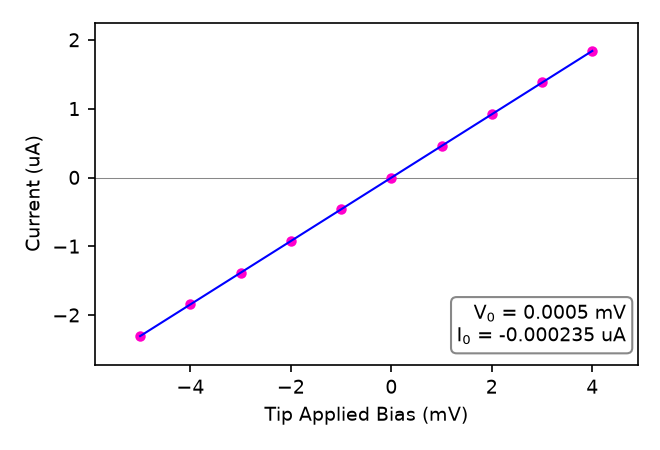
\includegraphics[width=0.9\linewidth]{../manual/figures/gui/Izero.png}
\\[2pt]{\small The Izero window after Find Offset on the simulator: the measured current at each applied bias (Igor's CurrentWave, pink markers), the fitted line (fit\_CurrentWave, blue), and the V0 / I0 box Igor drew with a TextBox.}
\end{center}

\section{Why it is measured in contact}

A line can only be fitted through a current that is measurable. Out of contact, 5 mV across a tunnelling gap gives picoamps of current and a slope made of noise. In contact the junction is a few k$\Omega$, the current at 5 mV is microamps, and the intercept is clean. That is why every point re-checks contact first --- a junction that breaks halfway through the sweep would otherwise fit a line through two regimes --- and why the routine has to restore your bias afterwards: it has been driving the junction at voltages you did not ask for.

It is also why the button belongs \emph{after} Start Approach in the lab sequence and before the run: the tip must be able to reach the surface, and the number is only worth having if it is applied to what follows.

\section{V0 check ON}

The checkbox is Igor's \texttt{Vzero\discretionary{}{}{}Check\discretionary{}{}{}Box}, read in two places by \texttt{Create\discretionary{}{}{}Inputs} and in one by \texttt{Single\discretionary{}{}{}Break\discretionary{}{}{}Junction\discretionary{}{}{}Attempt}:

\begin{itemize}[leftmargin=*]
\item \textbf{Constant-bias mode} (Functions\_STMBJ.ipf:1609-1614): with the box ticked the applied bias wave became \texttt{-(Tip\discretionary{}{}{}Bias + Vzero)/\discretionary{}{}{}1000} instead of \texttt{-(Tip\discretionary{}{}{}Bias)/\discretionary{}{}{}1000}. Now: \texttt{\_\discretionary{}{}{}measure\_\discretionary{}{}{}impl} passes \texttt{vzero\_\discretionary{}{}{}tracker.\discretionary{}{}{}offset\_\discretionary{}{}{}v} (V0 in volts, 0 if nothing has been measured) into \texttt{trace.\discretionary{}{}{}build\_\discretionary{}{}{}ramp(bias\_\discretionary{}{}{}offset\_\discretionary{}{}{}v=.\discretionary{}{}{}.\discretionary{}{}{}.\discretionary{}{}{})}, which adds it to the DC baseline only. The alignment spike stays at +Tip Bias, as Igor's line 1631 wrote it, so trace alignment does not depend on the offset. The bias recorded per trace in the session file is \texttt{bias\_\discretionary{}{}{}v + offset}, so a later reader knows what was actually applied.
\item \textbf{High-bias-hold mode} (lines 1595-1599): with the box ticked the hold bias \emph{became} the offset, \texttt{HBBias = Vzero/\discretionary{}{}{}1000} --- the zero-field control for the high-field runs. Now: \texttt{\_\discretionary{}{}{}build\_\discretionary{}{}{}ramp} passes \texttt{opts.\discretionary{}{}{}vzero\_\discretionary{}{}{}mv} into \texttt{ramps.\discretionary{}{}{}build\_\discretionary{}{}{}hb\_\discretionary{}{}{}hold(vzero\_\discretionary{}{}{}mv=.\discretionary{}{}{}.\discretionary{}{}{}.\discretionary{}{}{})}, whose \texttt{meta["from\_\discretionary{}{}{}vzero"]} records that it did.
\item \textbf{Push-pull, IV, AC hold}: no effect, in Igor or here.
\item \textbf{After every saved trace} (\texttt{Save\discretionary{}{}{}Offset}, line 993, called from \texttt{Single\discretionary{}{}{}Break\discretionary{}{}{}Junction\discretionary{}{}{}Attempt} at 1649): Igor re-measured the offset every \texttt{G\_\discretionary{}{}{}Vzero\discretionary{}{}{}Frequency} saved traces and appended the result to \texttt{Offset\discretionary{}{}{}Wave}, \texttt{Izero\discretionary{}{}{}Wave} and \texttt{Pull\discretionary{}{}{}Out\discretionary{}{}{}Number\discretionary{}{}{}Wave}, then called \texttt{Create\discretionary{}{}{}Inputs} again so the new V0 was in the next trace's bias. Now: \texttt{Vzero\discretionary{}{}{}Tracker.\discretionary{}{}{}maybe\_\discretionary{}{}{}measure (rig,\discretionary{}{}{} Saved)} runs after each accepted constant-mode trace, measures when \texttt{Saved \% every\_\discretionary{}{}{}n\_\discretionary{}{}{}traces == 0}, and the next \texttt{build\_\discretionary{}{}{}ramp} picks up \texttt{tracker.\discretionary{}{}{}offset\_\discretionary{}{}{}v}. Each measurement goes through the same \texttt{\_\discretionary{}{}{}record\_\discretionary{}{}{}vzero}, so the panel, the Izero window and the Izero\_Time window all update mid-run.
\end{itemize}

The tracker's history is written into the session file's summary as \texttt{vzero\_\discretionary{}{}{}history} (arrays of \texttt{vzero\_\discretionary{}{}{}mv}, \texttt{izero\_\discretionary{}{}{}a}, \texttt{timestamp}; chapter 47), which is the equivalent of Igor's three waves.

\begin{center}
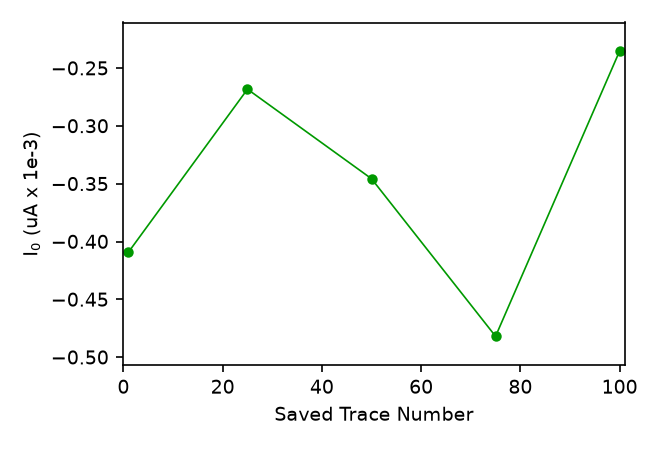
\includegraphics[width=0.9\linewidth]{../manual/figures/gui/Izero_Time.png}
\\[2pt]{\small Izero\_Time on the simulator with V0 check ON and Frequency set to 25 during a 100-trace run: one Find Offset before the run and four re-measurements, plotted against the Saved number at which each was taken. Igor's prescaleExp(left)=3 put the axis in \textmu{}A $\times$ 10⁻³, kept here.}
\end{center}

\section{The history is the diagnostic}

A single V0 is a correction. A \emph{series} of them is a measurement of the rig: an offset that drifts steadily over a session says the amplifier is warming, the electrolyte is changing, or the tip is ageing --- long before the histogram shows it. Igor plotted \texttt{Izero\discretionary{}{}{}Wave} against \texttt{Pull\discretionary{}{}{}Out\discretionary{}{}{}Number\discretionary{}{}{}Wave} for exactly this reason, and the Izero\_Time window is that plot. Leave V0 check ON with a Frequency of 50 for any run that cares about the low-bias region, and look at the window before trusting the day's data.

\section{Pitfalls}

\begin{itemize}[leftmargin=*]
\item \textbf{Pressing Find Offset before Start Writing} refuses with \texttt{the output task is not running -- press Start Writing first}.
\item \textbf{Before Start Approach}, on a real rig, the fine piezo cannot reach the surface; \texttt{\_\discretionary{}{}{}ensure\_\discretionary{}{}{}contact} climbs to the ceiling and refuses (message above). On the simulator the surface happens to be within reach from park, so this step is optional there.
\item \textbf{At the piezo floor.} The routine steps \emph{in}; it does not step out. If the tip is already in hard contact it fits a line through a metallic contact, which is fine --- a few k$\Omega$ is exactly what it wants.
\item \textbf{Simulator numbers.} The simulated card has a current offset but no bias offset, so V0 comes out at microvolts of noise. Do not read the simulator's V0 as a test of the fit; read the Izero window's straight line as one.
\item \textbf{Zero check on the Keithley} must be off (Keithley Controls) for the current to be real; Igor ticked it on at every Kill Tasks and left it to you to untick.
\item \textbf{The offset is not the preamp zero.} \texttt{calibrate.\discretionary{}{}{}measure\_\discretionary{}{}{}zero} (run at Start Writing) measures the amplifier's \emph{output} at zero bias out of contact and stores it as \texttt{cal.\discretionary{}{}{}current\_\discretionary{}{}{}zero\_\discretionary{}{}{}v}, which every conductance subtracts. V0 is the \emph{input} offset expressed as a bias, measured in contact, and is added to the applied bias. Both are needed; they correct different things.
\end{itemize}

% ==== 44_gui_echem_panel ====
\setcounter{chapter}{43}
\chapter{The Electrochemistry panel}

\begin{keybox}\small Igor: \texttt{EChem()} panel, Windows\_STMBJ.ipf:436-473; EChem\_Module.ipf. Modules: \texttt{stmgui/\discretionary{}{}{}panels/\discretionary{}{}{}echem\_\discretionary{}{}{}panel.\discretionary{}{}{}py}, \texttt{stmlab/\discretionary{}{}{}echem.\discretionary{}{}{}py}.\end{keybox}

Igor's EChem module did two unrelated things through one panel: it held a DC potential on a counter electrode while break-junction traces were taken (electrochemical gating), and it ran cyclic voltammetry by driving a triangle wave out of one card and recording the tip current. The panel has the same two group boxes --- \textbf{Electrochemical Gating} and \textbf{Cyclic Voltammetry} --- with Igor's controls in each. Chapter 15 is the physics and the command-line version (\texttt{experiments/\discretionary{}{}{}06\_\discretionary{}{}{}echem\_\discretionary{}{}{}gate\_\discretionary{}{}{}cv}); this chapter is the panel.

\begin{keybox}
Nothing in this panel has ever driven a real second card or a real cell from this code. The simulator exercises every line; the hardware paths are transcriptions of Igor's calls. Bring up on the scope first.
\end{keybox}

\section{Electrochemical Gating}

\small\setlength{\LTleft}{0pt}\setlength{\LTright}{\fill}
\begin{longtable}{@{}>{\raggedright\arraybackslash}p{0.230\linewidth}>{\raggedright\arraybackslash}p{0.230\linewidth}>{\raggedright\arraybackslash}p{0.230\linewidth}>{\raggedright\arraybackslash}p{0.230\linewidth}@{}}
\toprule
\textbf{Igor name} & \textbf{Title} & \textbf{Igor proc} & \textbf{Does now} \\
\midrule\endhead
\texttt{Start\discretionary{}{}{}EChem\discretionary{}{}{}Write\discretionary{}{}{}Button} & Counter Electrode ON & \texttt{Counter\discretionary{}{}{}Electrode\discretionary{}{}{}On} $\rightarrow$ \texttt{Start\discretionary{}{}{}EChem\discretionary{}{}{}Writing} & \texttt{Rig\discretionary{}{}{}Controller.\discretionary{}{}{}counter\_\discretionary{}{}{}electrode\_\discretionary{}{}{}on} \\
\texttt{Counter\discretionary{}{}{}Electrode\discretionary{}{}{}Set\discretionary{}{}{}Var} & Counter Electrode Bias (mV) & \texttt{Counter\discretionary{}{}{}Electrode\discretionary{}{}{}Set\discretionary{}{}{}Var} $\rightarrow$ \texttt{Write\discretionary{}{}{}To\discretionary{}{}{}Counter\discretionary{}{}{}Electrode} & \texttt{set\_\discretionary{}{}{}counter\_\discretionary{}{}{}electrode(mv)}; \texttt{cfg.\discretionary{}{}{}echem.\discretionary{}{}{}gate\_\discretionary{}{}{}mv} \\
\bottomrule
\end{longtable}
\normalsize

\textbf{Igor} created an output task on the low-res card's \texttt{ao1} (\texttt{Low\discretionary{}{}{}Res\discretionary{}{}{}Counter\discretionary{}{}{}Electrode\discretionary{}{}{}Out = "dev2/\discretionary{}{}{}ao1"}, Setup1\_STMBJ.ipf:11) with a $\pm$5 V range, wrote the current \texttt{G\_\discretionary{}{}{}Counter\discretionary{}{}{}Electrode\discretionary{}{}{}Bias}, then greyed the button and enabled the entry (EChem\_Module.ipf:41-48). Typing a new bias wrote it at once. \texttt{Stop\discretionary{}{}{}Writing\discretionary{}{}{}Tasks} and \texttt{EChem\discretionary{}{}{}Reset\discretionary{}{}{}DAQDevices} reversed the enable states and reset the card.

\textbf{Now}, Counter Electrode ON calls \texttt{stmlab.\discretionary{}{}{}echem.\discretionary{}{}{}make\_\discretionary{}{}{}counter\_\discretionary{}{}{}electrode (cfg).\discretionary{}{}{}on()} --- a \texttt{Simulated\discretionary{}{}{}Counter\discretionary{}{}{}Electrode} in simulate, otherwise a \texttt{Counter\discretionary{}{}{}Electrode} that opens an \texttt{nidaqmx} task on \texttt{\{channels.\discretionary{}{}{}low\_\discretionary{}{}{}res\_\discretionary{}{}{}device\}/\discretionary{}{}{}\{echem.\discretionary{}{}{}counter\_\discretionary{}{}{}electrode\_\discretionary{}{}{}channel\}} with \texttt{min\_\discretionary{}{}{}val=-5.\discretionary{}{}{}0,\discretionary{}{}{} max\_\discretionary{}{}{}val=5.\discretionary{}{}{}0}, as Igor's \texttt{MXCreate\discretionary{}{}{}AOVoltage\discretionary{}{}{}Chan(-5,\discretionary{}{}{}5)} --- and then writes the bias currently in the entry. If \texttt{channels.\discretionary{}{}{}low\_\discretionary{}{}{}res\_\discretionary{}{}{}device} is \texttt{None}, which is this one-card rig's default, it refuses with \texttt{EChem\discretionary{}{}{}Error: no low-res device configured (channels.\discretionary{}{}{}low\_\discretionary{}{}{}res\_\discretionary{}{}{}device is None); the counter electrode lives on the second card}. \texttt{--simulate} pretends a \texttt{Dev2} so the panel can be exercised.

After ON the button greys, the entry wakes, and every committed value goes to \texttt{Counter\discretionary{}{}{}Electrode.\discretionary{}{}{}set\_\discretionary{}{}{}mv}, which writes \texttt{mv/\discretionary{}{}{}1000} volts and stores the value in \textbf{\texttt{cfg.\discretionary{}{}{}echem.\discretionary{}{}{}gate\_\discretionary{}{}{}mv}} --- so the gate potential travels in the \texttt{config\_\discretionary{}{}{}json} of every session file written while it is applied. That is the point of doing it through the config rather than a local variable: a trace file taken under gate says so.

The entry is refused before ON with \texttt{press Counter Electrode ON first}. \textbf{Kill Tasks} releases the gate (\texttt{Counter\discretionary{}{}{}Electrode.\discretionary{}{}{}off()}, which writes 0 V, closes the task and zeroes \texttt{cfg.\discretionary{}{}{}echem.\discretionary{}{}{}gate\_\discretionary{}{}{}mv}) and puts the panel back to its starting state; \textbf{Reset DAQ Devices} does the same after resetting the cards, as Igor's \texttt{EChem\discretionary{}{}{}Reset\discretionary{}{}{}DAQDevices} set \texttt{Counter\discretionary{}{}{}Electrode\discretionary{}{}{}Bias = 0} (Controls\_STMBJ.ipf:228). Both emit a \texttt{gate} event with \texttt{None}, which is what the panel listens for.

A gate that should outlive the process --- set from a script, then left standing while the command-line experiment runs --- is \texttt{off(zero=False)} in the module; the GUI never does that, because the panel is the process.

\section{Cyclic Voltammetry}

\small\setlength{\LTleft}{0pt}\setlength{\LTright}{\fill}
\begin{longtable}{@{}>{\raggedright\arraybackslash}p{0.26\linewidth}>{\raggedright\arraybackslash}p{0.30\linewidth}>{\raggedright\arraybackslash}p{0.34\linewidth}@{}}
\toprule
\textbf{Igor name} & \textbf{Title} & \textbf{Bound to} \\
\midrule\endhead
\texttt{Set\discretionary{}{}{}Gain} & Gain ( log(V/A) ) & \texttt{cfg.\discretionary{}{}{}keithley.\discretionary{}{}{}gain\_\discretionary{}{}{}exponent} and \texttt{cfg.\discretionary{}{}{}cal.\discretionary{}{}{}preamp\_\discretionary{}{}{}gain\_\discretionary{}{}{}v\_\discretionary{}{}{}per\_\discretionary{}{}{}a} (the same entry as on the main panel) \\
\texttt{CVAcquisition\discretionary{}{}{}Rate\discretionary{}{}{}Set\discretionary{}{}{}Var} & CV Acquisition Rate (samps/s) & \texttt{cfg.\discretionary{}{}{}echem.\discretionary{}{}{}cv\_\discretionary{}{}{}rate\_\discretionary{}{}{}hz} (50 \ldots{} 40000, default 1000) \\
\texttt{Num\discretionary{}{}{}CVCycles\discretionary{}{}{}Set\discretionary{}{}{}Var} & Number of Cycles & \texttt{cfg.\discretionary{}{}{}echem.\discretionary{}{}{}cycles} (default 1) \\
\texttt{Scan\discretionary{}{}{}Rate\discretionary{}{}{}Set\discretionary{}{}{}Var} & Scan Rate (mV/s) & \texttt{cfg.\discretionary{}{}{}echem.\discretionary{}{}{}scan\_\discretionary{}{}{}rate\_\discretionary{}{}{}mv\_\discretionary{}{}{}per\_\discretionary{}{}{}s} (0 \ldots{} 2000 in steps of 25, default 100) \\
\texttt{Voltage\discretionary{}{}{}Peak\discretionary{}{}{}One\discretionary{}{}{}Set\discretionary{}{}{}Var} & Voltage Peak 1 (V) & \texttt{cfg.\discretionary{}{}{}echem.\discretionary{}{}{}peak\_\discretionary{}{}{}one\_\discretionary{}{}{}v} (−2.5 \ldots{} 0 in steps of 0.25, default −1) \\
\texttt{Voltage\discretionary{}{}{}Peak\discretionary{}{}{}Two\discretionary{}{}{}Set\discretionary{}{}{}Var} & Voltage Peak 2 (V) & \texttt{cfg.\discretionary{}{}{}echem.\discretionary{}{}{}peak\_\discretionary{}{}{}two\_\discretionary{}{}{}v} (0 \ldots{} 2.5 in steps of 0.25, default 1) \\
\texttt{Start\discretionary{}{}{}CVHigh\discretionary{}{}{}Res\discretionary{}{}{}Button} & CV HighRes & \texttt{start\_\discretionary{}{}{}cv("highres")} \\
\texttt{Start\discretionary{}{}{}CVLow\discretionary{}{}{}Res\discretionary{}{}{}Button} & CV LowRes & \texttt{start\_\discretionary{}{}{}cv("lowres")} \\
\bottomrule
\end{longtable}
\normalsize

Igor's five SetVariable procedures (\texttt{Voltage\discretionary{}{}{}Peak\discretionary{}{}{}One\discretionary{}{}{}Set\discretionary{}{}{}Var} and friends, EChem\_Module.ipf:414-466) each copied the typed value into its global; the bindings do that directly.

\subsection{The two buttons}

Igor enabled both CV buttons only after \texttt{Set\discretionary{}{}{}Gain} had run (Controls\_STMBJ.ipf:314-315) and disabled them again at \texttt{Stop\discretionary{}{}{}Writing\discretionary{}{}{}Tasks} (lines 204-205). The reason is worth keeping: a voltammogram is a current, and the current is the amplifier's output divided by a gain the analysis has to know. So the buttons are greyed until the Gain entry (either copy) has been committed once in this launch, and greyed again by Kill Tasks.

\textbf{CV HighRes} (\texttt{CVcurve\discretionary{}{}{}High\discretionary{}{}{}Res}, EChem\_Module.ipf:106) drove the triangle out of the \emph{high-res card's bias channel} --- \texttt{dev1/\discretionary{}{}{}ao1}, the same output the break-junction bias uses --- with the tip as working electrode, and read both \texttt{ai0} (the electrode voltage) and \texttt{ai1} (the tip current). \textbf{CV LowRes} (\texttt{CVcurve\discretionary{}{}{}Low\discretionary{}{}{}Res}, line 234) drove it out of the low-res card's counter-electrode channel with a $\pm$10 V range and read the tip current only. \texttt{stmlab.\discretionary{}{}{}echem.\discretionary{}{}{}run\_\discretionary{}{}{}cv(cfg,\discretionary{}{}{} kind)} does the same two things:

\begin{itemize}[leftmargin=*]
\item \texttt{kind="highres"}: \texttt{build\_\discretionary{}{}{}cv\_\discretionary{}{}{}ramp\_\discretionary{}{}{}highres} builds the wave (below); on hardware \texttt{\_\discretionary{}{}{}run\_\discretionary{}{}{}cv\_\discretionary{}{}{}hardware} opens an AO task on \texttt{channels.\discretionary{}{}{}path(ao\_\discretionary{}{}{}bias)} with a range wide enough for both peaks, an AI task on both input channels, both finite at \texttt{cv\_\discretionary{}{}{}rate\_\discretionary{}{}{}hz}, and --- one deliberate improvement --- starts the AI on the AO's start trigger, where Igor started the two tasks back to back and lived with the skew. Each cycle returns a \texttt{CVCycle} with \texttt{applied\_\discretionary{}{}{}v}, \texttt{tip\_\discretionary{}{}{}current\_\discretionary{}{}{}v} (raw preamp volts), \texttt{we\_\discretionary{}{}{}voltage\_\discretionary{}{}{}mv} (the measured electrode voltage) and \texttt{keep}.
\item \texttt{kind="lowres"}: \texttt{build\_\discretionary{}{}{}cv\_\discretionary{}{}{}ramp\_\discretionary{}{}{}lowres} (5000 samples of 0 V first, then the triangle with a longer repeated tail, Igor lines 251-286); the AO task on the second card's counter-electrode channel at $\pm$10 V; tip current only, \texttt{we\_\discretionary{}{}{}voltage\_\discretionary{}{}{}mv} is \texttt{None}.
\end{itemize}

In simulate, \texttt{\_\discretionary{}{}{}run\_\discretionary{}{}{}cv\_\discretionary{}{}{}simulated} replaces the cell with a model: a 1 \textmu{}F double-layer capacitance whose current flips sign with the scan direction (the rectangular part of the loop) and one reversible couple with anodic and cathodic peaks 60 mV apart around +0.2 V, plus noise. Not chemistry --- shape, enough to test every line of the analysis and the plot.

\subsection{The ramp and the keep mask}

Igor's high-res wave (lines 127-158) was 0 $\rightarrow$ Peak 1 $\rightarrow$ 0 $\rightarrow$ Peak 2 $\rightarrow$ 0, then the first half again, and it NaN-ed the first quarter (the switch-on transient) and the repeated half so that what remained was one closed cycle starting and ending at the same potential. \texttt{build\_\discretionary{}{}{}cv\_\discretionary{}{}{}ramp\_\discretionary{}{}{}highres} builds exactly that wave, with the number of samples per leg from \texttt{2 × |peak| /\discretionary{}{}{} scan\_\discretionary{}{}{}rate × cv\_\discretionary{}{}{}rate\_\discretionary{}{}{}hz}, and returns beside it a boolean \texttt{keep} that is \texttt{False} where Igor wrote NaN. Keeping the mask \emph{beside} the complete record instead of destroying the samples means a later reader can second-guess the choice. A ramp with fewer than four samples per leg is refused: \texttt{CV ramp too short; slow the scan rate or raise cv\_\discretionary{}{}{}rate\_\discretionary{}{}{}hz}.

\subsection{What the button does around the sweep}

\texttt{Start\discretionary{}{}{}CVHigh\discretionary{}{}{}Res\discretionary{}{}{}Button} (EChem\_Module.ipf:364-387) checked the main panel's Zero Check box, sent \texttt{C0X} to lift zero check if it was ticked, ran the sweep, and sent \texttt{C1X} to put it back. \texttt{Rig\discretionary{}{}{}Controller.\discretionary{}{}{}\_\discretionary{}{}{}cv\_\discretionary{}{}{}impl} does the same: if \texttt{opts.\discretionary{}{}{}zero\_\discretionary{}{}{}check} is set and the Keithley is connected, zero check is lifted, the sweep runs inside a \texttt{try}, and zero check is restored in the \texttt{finally}.

One refusal Igor did not have: on hardware, \textbf{CV HighRes while the output task is running} is refused with \texttt{CV High\discretionary{}{}{}Res drives the junction-bias channel; Kill Tasks first (Igor reset the card afterwards)}. Two tasks cannot own \texttt{dev1/\discretionary{}{}{}ao1} at once; Igor let them collide and then \texttt{MXReset\discretionary{}{}{}Device}'d the card. In simulate there is nothing to collide with and the refusal is not raised.

After the sweep, \texttt{storage.\discretionary{}{}{}save\_\discretionary{}{}{}cv\_\discretionary{}{}{}cycles} writes \texttt{data/\discretionary{}{}{}<date>/\discretionary{}{}{}cv\_\discretionary{}{}{}<kind>\_\discretionary{}{}{}<HHMMSS>.\discretionary{}{}{}h5} (layout in chapter 47), the cycles are kept as \texttt{controller.\discretionary{}{}{}last\_\discretionary{}{}{}cv}, and a \texttt{cv} event opens or redraws the CyclicVoltammogram window.

\begin{center}
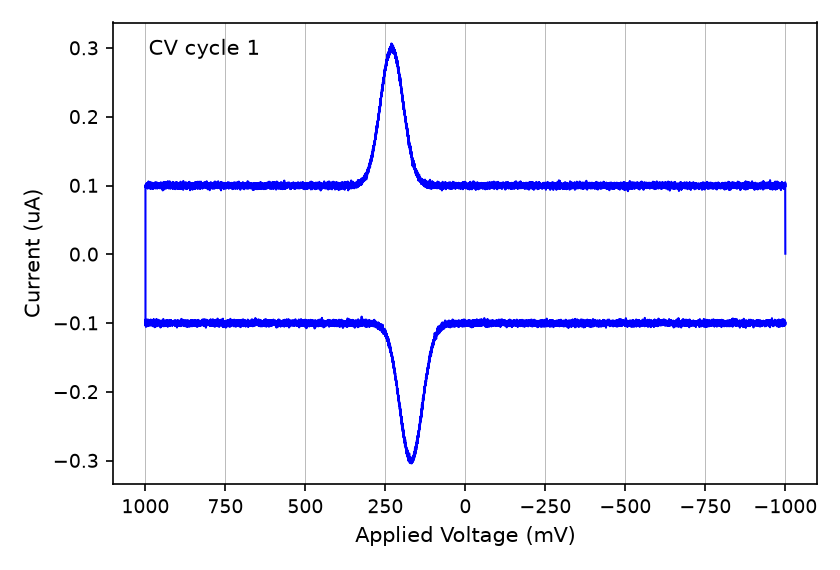
\includegraphics[width=0.9\linewidth]{../manual/figures/gui/CyclicVoltammogram.png}
\\[2pt]{\small The Cyclic Voltammogram window after CV HighRes on the simulator: tip current in \textmu{}A against applied potential in mV, x axis reversed as Igor's SetAxis/A/R bottom had it, the masked switch-on quarter and repeated tail left out. The rectangle is the double-layer current; the pair of peaks is the model couple.}
\end{center}

\subsection{Reading the numbers}

The plotted current is \texttt{tip\_\discretionary{}{}{}current\_\discretionary{}{}{}v /\discretionary{}{}{} cal.\discretionary{}{}{}preamp\_\discretionary{}{}{}gain\_\discretionary{}{}{}v\_\discretionary{}{}{}per\_\discretionary{}{}{}a}, in \textmu{}A. With the default gain of 10⁶ V/A, 0.1 \textmu{}A of double-layer current is 0.1 V at the ADC; a real cell with a large electrode can put out far more, and a railed channel shows as a flat top at $\pm$10 V. Lower the gain (the Gain entry on this panel) before a CV on a real cell, and remember that the same entry sets the gain the break-junction conductance divides by --- put it back before the next Start Measurement, or \texttt{validate()} will tell you about the mismatch in the History.

\section{Between the two groups}

Igor's gating and CV were independent --- you could gate while measuring traces and never run a CV, or run CVs with no gate. The same holds here, with one practical link: on hardware a CV HighRes needs the output task off, so the sequence for a gated voltammogram on this rig is Counter Electrode ON, set the bias, Kill Tasks if the task was running, CV HighRes, then Start Writing again for traces.

% ==== 45_gui_graphs ====
\setcounter{chapter}{44}
\chapter{The graph windows and the History window}

\begin{keybox}\small Igor: the Graph macros in Windows\_STMBJ.ipf:33-131, 407-434 and 475-489; the history area. Modules: \texttt{stmgui/\discretionary{}{}{}graphs.\discretionary{}{}{}py}, \texttt{stmgui/\discretionary{}{}{}panels/\discretionary{}{}{}history.\discretionary{}{}{}py}.\end{keybox}

Igor's experiment showed its data in nine small graph windows, each a macro that displayed one or two waves with fixed axes, and printed its commentary into the history area. All ten are here. Each graph is a matplotlib figure in its own Tk window (\texttt{Graph\discretionary{}{}{}Window}), created the first time it is needed, hidden rather than destroyed when closed, and listed under the \textbf{Windows} menu. Every figure in this chapter was produced by the window itself, on the simulator, by \texttt{manual\_\discretionary{}{}{}build/\discretionary{}{}{}make\_\discretionary{}{}{}figures.\discretionary{}{}{}py}.

\section{How the windows get their data}

The controller posts events; \texttt{Graph\discretionary{}{}{}Set.\discretionary{}{}{}on\_\discretionary{}{}{}event} routes them. The table is \texttt{Graph\discretionary{}{}{}Set.\discretionary{}{}{}FEEDS}:

\small\setlength{\LTleft}{0pt}\setlength{\LTright}{\fill}
\begin{longtable}{@{}>{\raggedright\arraybackslash}p{0.26\linewidth}>{\raggedright\arraybackslash}p{0.30\linewidth}>{\raggedright\arraybackslash}p{0.34\linewidth}@{}}
\toprule
\textbf{Event} & \textbf{Windows fed} & \textbf{Fired by} \\
\midrule\endhead
\texttt{highres} & HighRes & every background read \\
\texttt{trace} & PullOutLowG, PullOutGvsE, AuAuConductanceLevel, SenseInDisplay & every generated trace, saved or not \\
\texttt{hist} & LogHistOfBlock & every 100 saved traces, and the partial block at the end of a run \\
\texttt{izero} & Izero & Find Offset, and each periodic re-measure \\
\texttt{izero\_\discretionary{}{}{}time} & Izero\_Time & the same \\
\texttt{cv} & CyclicVoltammogram & each CV run \\
\bottomrule
\end{longtable}
\normalsize

The first time an event reaches a window that does not yet exist, the window is created and --- for the first-listed window of each event, and always for Izero, LogHistOfBlock and CyclicVoltammogram --- shown. That is Igor's \texttt{Do\discretionary{}{}{}Window/\discretionary{}{}{}F name; if (V\_\discretionary{}{}{}flag==0) Execute "name()"} idiom, which opened a graph on first use and thereafter just brought it forward. The three secondary trace windows (PullOutGvsE, AuAuConductanceLevel, SenseInDisplay) are created and kept up to date but not raised, to keep the first run from covering the screen; open them from the Windows menu.

Updates happen on the Tk thread, at most every 50 ms, from the event pump (chapter 48). A run on the simulator generates traces faster than that, so the pull-out windows show every trace but not every one is rendered before the next arrives; on hardware, at one trace per second or so, every one is.

\section{HighRes}

\textbf{Igor:} \texttt{High\discretionary{}{}{}Res()}, Windows\_STMBJ.ipf:33 --- \texttt{Voltage\discretionary{}{}{}In} (blue) and \texttt{Voltage\discretionary{}{}{}In\discretionary{}{}{}Low\discretionary{}{}{}Res} (orange) against the left axis in mV, \texttt{Current\discretionary{}{}{}In\discretionary{}{}{}Low\discretionary{}{}{}Res} (pink) and \texttt{Current\discretionary{}{}{}In} (green) against the right axis in \textmu{}A; the last background read from both cards.

\textbf{Now:} the last background read from the one card: junction voltage in mV (\texttt{voltage\_\discretionary{}{}{}input\_\discretionary{}{}{}sign × V × 1000}) on the left axis in Igor's blue, tip current in \textmu{}A (\texttt{volts\_\discretionary{}{}{}to\_\discretionary{}{}{}amps(I) × 10⁶}) on the right axis in Igor's green, against sample number. \textbf{Fast Read Wave Size} sets the length. Axes autoscale to the data with a 10 \% margin and never use matplotlib's offset notation, so 100.02 mV reads as 100.02, not +0.02 over 1e2. There is no low-res pair because there is no low-res card.

\begin{center}
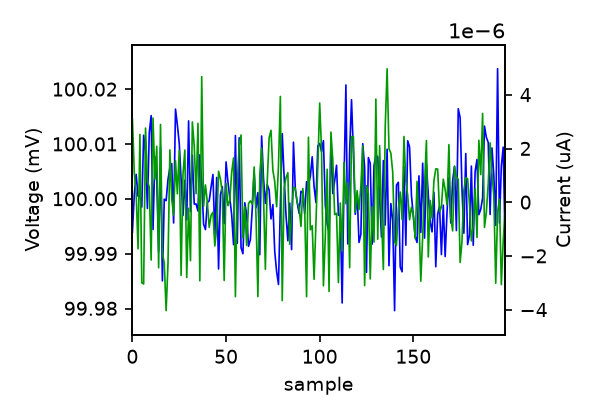
\includegraphics[width=0.9\linewidth]{../manual/figures/gui/HighRes.png}
\\[2pt]{\small HighRes on the simulator, in contact after Start Approach: 200 samples of junction voltage around −100 mV (the bias is applied as −TipBias, so the measured, sign-corrected voltage is −100 mV) and a current of about 10 \textmu{}A. Retracted, the current trace is noise around zero.}
\end{center}

\section{PullOutGvsE, PullOutLowG, AuAuConductanceLevel}

Three views of the same wave. Igor's \texttt{Pull\discretionary{}{}{}Out\discretionary{}{}{}Conductance} was the conductance of the last generated trace in units of G0 against displacement in nm; \texttt{Generate\discretionary{}{}{}Trace} filled it before \texttt{Test\discretionary{}{}{}Trace} judged the trace, so rejected traces were shown too. The same here: every \texttt{trace} event carries \texttt{g0} (from \texttt{Trace\discretionary{}{}{}Record.\discretionary{}{}{}conductance\_\discretionary{}{}{}g0}, i.e. the measured current over the measured voltage), \texttt{disp\_\discretionary{}{}{}nm} (the commanded piezo retraction from the contact point, \texttt{piezo\_\discretionary{}{}{}volts\_\discretionary{}{}{}to\_\discretionary{}{}{}nm(start − piezo)}), \texttt{bias\_\discretionary{}{}{}mv} (the measured junction voltage), \texttt{piezo\_\discretionary{}{}{}nm} (the absolute commanded position), the trace number, the mode, and whether it was saved. Each window prints \texttt{trace N saved (constant)} or \texttt{trace N rejected} in its corner.

\small\setlength{\LTleft}{0pt}\setlength{\LTright}{\fill}
\begin{longtable}{@{}>{\raggedright\arraybackslash}p{0.230\linewidth}>{\raggedright\arraybackslash}p{0.230\linewidth}>{\raggedright\arraybackslash}p{0.230\linewidth}>{\raggedright\arraybackslash}p{0.230\linewidth}@{}}
\toprule
\textbf{Window} & \textbf{Igor macro} & \textbf{Axis} & \textbf{Igor range} \\
\midrule\endhead
PullOutGvsE & \texttt{Pull\discretionary{}{}{}Out\discretionary{}{}{}Gvs\discretionary{}{}{}E()}, line 52 & linear G0 & from 0 upward, autoscaled \\
PullOutLowG & \texttt{Pull\discretionary{}{}{}Out\discretionary{}{}{}Low()}, line 66 & log G0 & 1e-6 to 5.58676 \\
AuAuConductanceLevel & \texttt{Au\discretionary{}{}{}Au\discretionary{}{}{}Conductance\discretionary{}{}{}Level()}, line 86 & linear G0 & 1e-5 to 5 \\
\bottomrule
\end{longtable}
\normalsize

\textbf{PullOutLowG} is the one you watch. The log axis spans the whole trace from metallic contact through the molecular plateau to tunnelling; the odd upper limit is Igor's own \texttt{Set\discretionary{}{}{}Axis left 1e-06,\discretionary{}{}{}5.\discretionary{}{}{}58676}. Igor also appended \texttt{Pull\discretionary{}{}{}Out\discretionary{}{}{}Voltage} --- the measured bias in mV --- on a right axis and hid it (\texttt{hide\discretionary{}{}{}Trace(Pull\discretionary{}{}{}Out\discretionary{}{}{}Voltage)=1}); the same trace is here, hidden, with a \textbf{show PullOutVoltage} checkbox under the plot to reveal it. Igor's window was titled "PullOutLowG"; so is this one.

\textbf{PullOutGvsE} is the linear view of the plateau region, y from 0 to a little above the trace's maximum (Igor: \texttt{Set\discretionary{}{}{}Axis left 0,\discretionary{}{}{}*}).

\textbf{AuAuConductanceLevel} is Igor's third view, linear from 1e-5 to 5 --- in practice the 1 G0 gold plateau at the left edge of the trace, which is what the name says.

\begin{center}
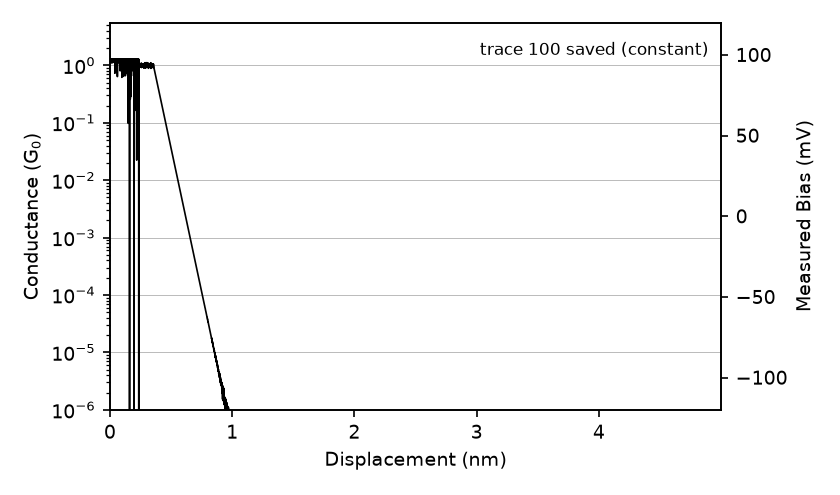
\includegraphics[width=0.9\linewidth]{../manual/figures/gui/PullOutLowG.png}
\\[2pt]{\small PullOutLowG on the simulator: the last saved trace of a 100-trace run. Metallic contact at the left, the gold plateau at 1 G0, then the exponential tunnelling descent to the noise floor; this particular trace caught no molecule, and one that does shows a second plateau three to four decades down. The measured-bias trace on the right axis is hidden, as in Igor.}
\end{center}

\begin{center}
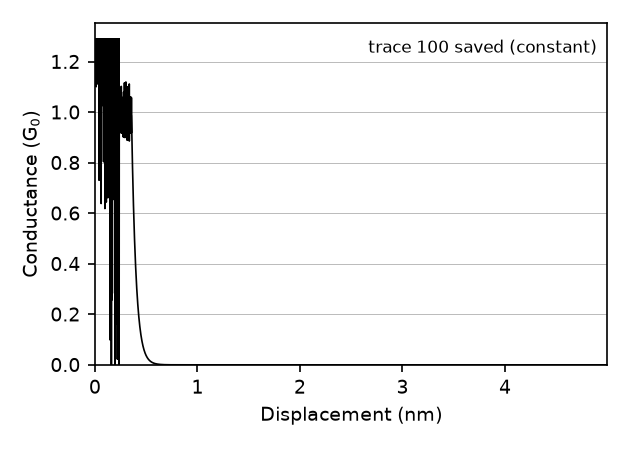
\includegraphics[width=0.9\linewidth]{../manual/figures/gui/PullOutGvsE.png}
\\[2pt]{\small PullOutGvsE, the same trace on a linear axis from 0.}
\end{center}

\begin{center}
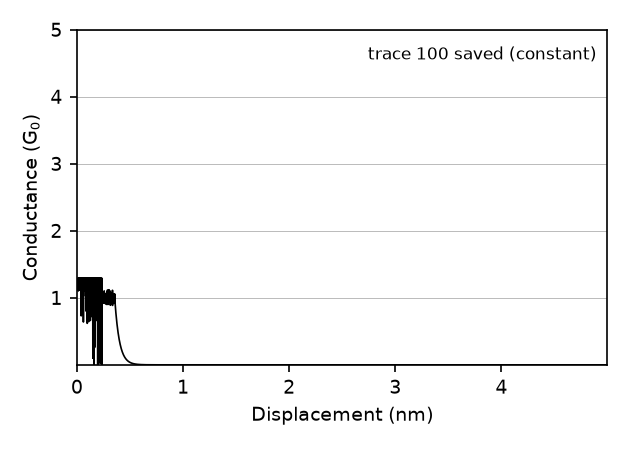
\includegraphics[width=0.9\linewidth]{../manual/figures/gui/AuAuConductanceLevel.png}
\\[2pt]{\small AuAuConductanceLevel, the same trace between 1e-5 and 5 G0.}
\end{center}

For the four ramp modes the displacement axis is still the commanded piezo position relative to contact, which for a push-pull cycle goes negative and comes back, and for a hold stays flat while the bias does the work. \texttt{Trace\discretionary{}{}{}Record.\discretionary{}{}{}displacement\_\discretionary{}{}{}nm}, which assumes a constant pull rate, is \emph{not} used for these windows for exactly that reason; the ramp's own waveform is.

\section{SenseInDisplay}

\textbf{Igor:} \texttt{Sense\discretionary{}{}{}In\discretionary{}{}{}Display()}, line 100 --- \texttt{Sense\discretionary{}{}{}In}, the piezo position in nm read back from the low-res card's sense input, against points.

\textbf{Now:} the \emph{commanded} piezo position in nm for the last trace, against sample number. This rig has one card and no sense line; the number shown is the same tracked command every safety check trusts. A straight descending line is a constant pull; a push-pull cycle shows its excursions; a hold shows a flat section. If you ever add a sense input, \texttt{Rig.\discretionary{}{}{}play} returns the record and this window is where the readback belongs.

\begin{center}
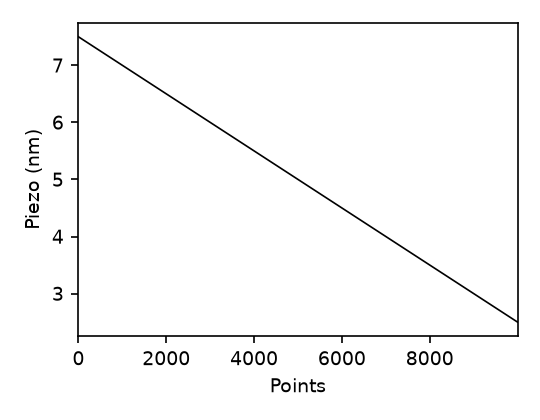
\includegraphics[width=0.9\linewidth]{../manual/figures/gui/SenseInDisplay.png}
\\[2pt]{\small SenseInDisplay for a constant pull: the commanded piezo descending at 20 nm/s from the contact point, 10 000 points at 40 kHz for a 5 nm excursion.}
\end{center}

\section{LogHistOfBlock}

\textbf{Igor:} \texttt{Log\discretionary{}{}{}Hist\discretionary{}{}{}Of\discretionary{}{}{}Block()}, line 113 --- \texttt{Log\discretionary{}{}{}Hist\discretionary{}{}{}Wave} as bars (\texttt{mode=7}, \texttt{hb\discretionary{}{}{}Fill=5}, blue), "Counts/Trace" against "Conductance [Log]", axes −6 \ldots{} 1 and 0 \ldots{} 40. \texttt{Log\discretionary{}{}{}Hist\discretionary{}{}{}From\discretionary{}{}{}Blocks} (Functions\_STMBJ.ipf:785) built it from each 100-trace \texttt{Conductance\discretionary{}{}{}Block} as it was saved: keep 95 \% of each trace, smooth, estimate the floor from the 95-96 \% window, drop the trace if the floor is above the zero cutoff, subtract, smooth, log10, histogram into 1000 bins from −8 to 2, divide by 100.

\textbf{Now:} \texttt{analysis.\discretionary{}{}{}log\_\discretionary{}{}{}histogram} on the block, called by the controller when the block reaches 100 saved traces (\texttt{HIST\_\discretionary{}{}{}BLOCK}) and again for whatever is left when a run ends (that second call is a GUI addition; Igor showed nothing until a block was complete). The zero cutoff is \texttt{cfg.\discretionary{}{}{}ramp.\discretionary{}{}{}break\_\discretionary{}{}{}g0}, Igor's \texttt{G\_\discretionary{}{}{}End\discretionary{}{}{}Of\discretionary{}{}{}Trace\discretionary{}{}{}Noise\discretionary{}{}{}Threshold}. For the ramp modes the hold or push-pull section is removed first --- Igor's \texttt{Deletepoints Start\discretionary{}{}{}Delete,\discretionary{}{}{} Number\discretionary{}{}{}To\discretionary{}{}{}Delete} --- using the ramp's segment table: everything between the end of the initial pull and the start of the final pull. The bars are Igor's blue; x is fixed at −6 \ldots{} 1; y starts at 0 \ldots{} 40 and grows if a peak exceeds it. The corner text says how many traces the block holds and whether it is partial. With \textbf{Save Hist} ticked, each block is also written as a CSV (chapter 47).

\begin{center}
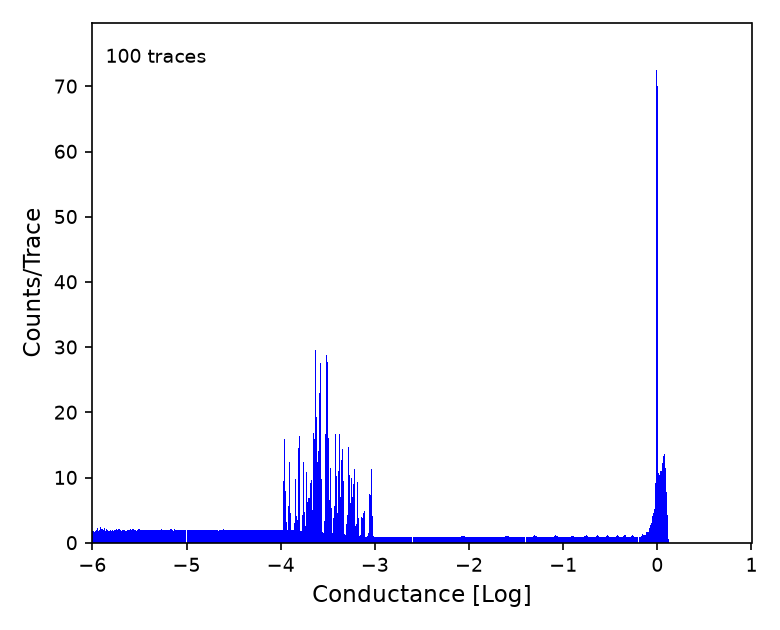
\includegraphics[width=0.9\linewidth]{../manual/figures/gui/LogHistOfBlock.png}
\\[2pt]{\small LogHistOfBlock after the first 100 saved traces on the simulator: the 1 G0 gold peak at log G = 0, the simulator's molecular peak around −3.5, and the tunnelling background.}
\end{center}

The histogram is the measurement. One trace proves nothing; a peak that recurs across a hundred does. Chapter 10 says why the floor estimate and the cutoff gate matter, and what a missing gold peak means (usually the gain).

\section{Izero and Izero\_Time}

\textbf{Igor:} \texttt{Izero()}, line 407 --- \texttt{Current\discretionary{}{}{}Wave} against \texttt{Tip\discretionary{}{}{}Bias\discretionary{}{}{}Ramp} as markers (pink) with \texttt{fit\_\discretionary{}{}{}Current\discretionary{}{}{}Wave} (blue), "Current (\textmu{}A)" against "Tip Applied Bias (mV)", a zero line, and a \texttt{Text\discretionary{}{}{}Box} with \texttt{G\_\discretionary{}{}{}Vzero} and \texttt{G\_\discretionary{}{}{}Izero}. \texttt{Izero\_\discretionary{}{}{}Time()}, line 421 --- \texttt{Izero\discretionary{}{}{}Wave} against \texttt{Pull\discretionary{}{}{}Out\discretionary{}{}{}Number\discretionary{}{}{}Wave} as connected markers (green), "I0 (\textmu{}A $\times$ 1e-3)" against "Saved Trace Number".

\textbf{Now:} \texttt{Izero} draws each \texttt{Vzero\discretionary{}{}{}Result} from Find Offset or a periodic re-measure --- points at \texttt{(bias\_\discretionary{}{}{}mv,\discretionary{}{}{} current\_\discretionary{}{}{}a × 10⁶)}, a \texttt{numpy.\discretionary{}{}{}polyfit} line through them, and the V0 / I0 box. \texttt{Izero\_\discretionary{}{}{}Time} draws the controller's \texttt{izero\_\discretionary{}{}{}history}, one \texttt{(Saved,\discretionary{}{}{} I0)} pair per measurement, in \textmu{}A $\times$ 10⁻³ as Igor's \texttt{prescale\discretionary{}{}{}Exp(left)=3} had it. Chapter 43 shows both figures and explains what to read in them.

\section{CyclicVoltammogram}

\textbf{Igor:} \texttt{Cyclic\discretionary{}{}{}Voltammogram()}, line 475 --- \texttt{Tip\discretionary{}{}{}Current} against \texttt{CVApplied\discretionary{}{}{}Ramp}, "Current (\textmu{}A)" against "Applied Voltage (mV)", x reversed (\texttt{Set\discretionary{}{}{}Axis/\discretionary{}{}{}A/\discretionary{}{}{}R bottom}), a "CV cycle N" text box.

\textbf{Now:} every cycle of the last CV, current \texttt{tip\_\discretionary{}{}{}current\_\discretionary{}{}{}v /\discretionary{}{}{} cal.\discretionary{}{}{}preamp\_\discretionary{}{}{}gain\_\discretionary{}{}{}v\_\discretionary{}{}{}per\_\discretionary{}{}{}a} in \textmu{}A against applied potential in mV, masked samples left out, earlier cycles in a lighter blue and the last cycle in Igor's blue, x reversed, the cycle number in the corner. Chapter 44 has the figure.

\section{The History window}

Igor printed to its history area --- every \texttt{Print}, every command echo --- and that record was the run's log. The \textbf{History} window is that: a scrolling text with one line per log record from the \texttt{stmlab} and \texttt{stmgui} loggers at INFO and above, routed there by \texttt{controller.\discretionary{}{}{}Queue\discretionary{}{}{}Log\discretionary{}{}{}Handler} as \texttt{log} events, plus every \texttt{error} event. Each line is stamped with the wall-clock time, then the level letter and the logger name, then the message:

\begin{lstlisting}[style=out]
15:28:30  -> Start Measurement: stmgui/controller.py:722 RigController._measure_impl
15:28:30  I stmlab.storage: writing to .../constant_152830_from1.h5
15:28:30  W stmgui.controller: config: hv_amp_gain is unknown; ...
15:28:31  ERROR Start Measurement: the output task is not running -- press Start Writing first
\end{lstlisting}

The \texttt{->} line is written by the worker as each command starts: the button name, then the file, line and function of the Python that is about to run --- so the History is also the answer to "which function did that button call". \texttt{W} lines are amber, \texttt{E} and \texttt{ERROR} lines red. The buffer keeps the last 5000 lines. Everything the chapters of this manual quote as "in the History" is a line here; if you want it on disk too, launch with \texttt{-v} and redirect the console, or read the session file's \texttt{run\_\discretionary{}{}{}stats\_\discretionary{}{}{}json} (chapter 47), which keeps the counts.

\section{Placement and size}

Igor positioned each window with its \texttt{Display /\discretionary{}{}{}W=(left,\discretionary{}{}{} top,\discretionary{}{}{} right,\discretionary{}{}{} bottom)}; \texttt{Graph\discretionary{}{}{}Set.\discretionary{}{}{}ORDER} keeps those origins, scaled to today's screens, and each window's \texttt{igor\_\discretionary{}{}{}geometry} is a size in the same spirit --- HighRes small, LogHistOfBlock large. Drag them where you like; positions are not remembered between launches, as Igor's were in the experiment file. The figures resize with their windows.

% ==== 46_gui_macros ====
\setcounter{chapter}{45}
\chapter{Menus and macros: rungo, LateralEXPT, the X piezo, config files}

\begin{keybox}\small Igor: the \texttt{Macros} menu, Setup1\_STMBJ.ipf:50; \texttt{rungo()}, :138; \texttt{Lateral\discretionary{}{}{}EXPT()}, :91; \texttt{Setup\discretionary{}{}{}XPiezo} / \texttt{Move\discretionary{}{}{}XPiezo} / \texttt{Move\discretionary{}{}{}XPiezo\discretionary{}{}{}To\discretionary{}{}{}Zero}, NanoPZ\_Actuator\_Functions\_STM.ipf:25-91. Module: \texttt{stmgui/\discretionary{}{}{}app.\discretionary{}{}{}py} (menus), \texttt{stmgui/\discretionary{}{}{}controller.\discretionary{}{}{}py} (the macros).\end{keybox}

Igor's menu bar had one item of its own --- \textbf{Macros $\rightarrow$ STM Break Junction Measurement}, which ran \texttt{Initialize\discretionary{}{}{}Experiment} --- and two procedures that were only ever typed into the command line: \texttt{rungo()}, the bias series, and \texttt{Lateral\discretionary{}{}{}EXPT(.\discretionary{}{}{}.\discretionary{}{}{}.\discretionary{}{}{})}, the monolayer walk. The rebuild has four menus. This chapter is what is in them.

\section{File}

\small\setlength{\LTleft}{0pt}\setlength{\LTright}{\fill}
\begin{longtable}{@{}>{\raggedright\arraybackslash}p{0.34\linewidth}>{\raggedright\arraybackslash}p{0.58\linewidth}@{}}
\toprule
\textbf{Item} & \textbf{Does} \\
\midrule\endhead
Load config JSON... & \texttt{Rig\discretionary{}{}{}Config.\discretionary{}{}{}from\_\discretionary{}{}{}json} into the live config; every panel refreshes \\
Save config JSON... & \texttt{Rig\discretionary{}{}{}Config.\discretionary{}{}{}to\_\discretionary{}{}{}json} of the live config \\
Open data folder & opens \texttt{data/\discretionary{}{}{}<today>/\discretionary{}{}{}} in the file browser \\
Quit & \texttt{controller.\discretionary{}{}{}shutdown()} --- Kill Tasks, release the Keithley --- then closes \\
\bottomrule
\end{longtable}
\normalsize

A saved config is the complete \texttt{Rig\discretionary{}{}{}Config} --- channels, limits, ramp, calibration, actuator, the four mode configs, vzero, keithley, echem, xpiezo, the simulate flag and notes --- as indented JSON. It is the same file \texttt{run.\discretionary{}{}{}py <experiment> --config my.\discretionary{}{}{}json} reads and the same dictionary every session file carries as \texttt{config\_\discretionary{}{}{}json}, so a config tuned at the panel runs unchanged from the command line, and a command-line config loads unchanged into the panel. What it does \emph{not} contain is \texttt{Gui\discretionary{}{}{}Options}: Saved, Stop \#, the checkbox states, Piezo offset, Fast Read Wave Size. Those are panel state, not rig description, and start fresh each launch (chapter 48 lists them).

Loading replaces every section of the live config in place, so the controller, the open \texttt{Rig} and the tracker all see the new values at once. Load before Start Writing; a config loaded under a running task takes effect at the next command that reads each field, which is consistent but rarely what you meant.

\section{Macros}

\small\setlength{\LTleft}{0pt}\setlength{\LTright}{\fill}
\begin{longtable}{@{}>{\raggedright\arraybackslash}p{0.26\linewidth}>{\raggedright\arraybackslash}p{0.30\linewidth}>{\raggedright\arraybackslash}p{0.34\linewidth}@{}}
\toprule
\textbf{Item} & \textbf{Igor} & \textbf{Does} \\
\midrule\endhead
STM Break Junction Measurement & \texttt{Initialize\discretionary{}{}{}Experiment} & raises the main panel \\
Voltage Offset panel & \texttt{Voltage\_\discretionary{}{}{}Offset()} & raises it (chapter 43) \\
Electrochemistry panel & \texttt{EChem()} & raises it (chapter 44) \\
rungo()  bias series... & \texttt{rungo()} & the bias campaign, below \\
LateralEXPT(Z, X, XFreq)... & \texttt{Lateral\discretionary{}{}{}EXPT} & the monolayer walk, below \\
MoveXPiezo(nm)... & \texttt{Move\discretionary{}{}{}XPiezo} & relative lateral move \\
MoveXPiezoToZero() & \texttt{Move\discretionary{}{}{}XPiezo\discretionary{}{}{}To\discretionary{}{}{}Zero} & lateral piezo to 0 V \\
Stop (Alt) & \texttt{Get\discretionary{}{}{}Key\discretionary{}{}{}State} & \texttt{request\_\discretionary{}{}{}stop} \\
\bottomrule
\end{longtable}
\normalsize

\subsection{rungo(): the bias series}

\textbf{Igor} (Setup1\_STMBJ.ipf:138-179) built three waves of fourteen entries: \texttt{bias} = −100, −200, \ldots{} −900, then −100, −900, −1000, −1100, −100 mV; \texttt{Stop\discretionary{}{}{}Num\discretionary{}{}{}Wave[i] = (i+1) × 1000 + 1}; \texttt{Start\discretionary{}{}{}Num\discretionary{}{}{}Wave = Stop\discretionary{}{}{}Num\discretionary{}{}{}Wave − 1000}. It then found where the current \texttt{G\_\discretionary{}{}{}Pull\discretionary{}{}{}Out\discretionary{}{}{}Number} fell in \texttt{Start\discretionary{}{}{}Num\discretionary{}{}{}Wave} (\texttt{Find\discretionary{}{}{}Level/\discretionary{}{}{}EDGE=1}) and, from that index on, set \texttt{G\_\discretionary{}{}{}Tip\discretionary{}{}{}Bias} and \texttt{G\_\discretionary{}{}{}Stop\discretionary{}{}{}Number} and called \texttt{Start\discretionary{}{}{}Measurement} --- so a campaign interrupted after 3400 saved traces resumed at step 3, bias −400 mV, and ran it to
\begin{enumerate}[leftmargin=*]
\item Two \texttt{Piezo\discretionary{}{}{}Step\discretionary{}{}{}Apart} calls and a \texttt{Find\discretionary{}{}{}Suppress} per step were commented out. Alt between steps aborted. At the end: \texttt{Save\discretionary{}{}{}Experiment} and \texttt{Stop\discretionary{}{}{}Writing\discretionary{}{}{}Tasks}.
\end{enumerate}

\textbf{Now}, Macros $\rightarrow$ rungo() asks two questions --- the bias list in mV, comma separated, pre-filled with Igor's fourteen values, and the number of traces per bias, pre-filled with 1000 --- and calls \texttt{Rig\discretionary{}{}{}Controller.\discretionary{}{}{}rungo(biases\_\discretionary{}{}{}mv,\discretionary{}{}{} counts\_\discretionary{}{}{}each)}. \texttt{\_\discretionary{}{}{}rungo\_\discretionary{}{}{}impl} computes the same \texttt{stop\_\discretionary{}{}{}nums} and \texttt{start\_\discretionary{}{}{}nums}, resumes from the last step whose start number is at or below the current Saved (the \texttt{Find\discretionary{}{}{}Level} logic), and for each remaining step logs \texttt{rungo step i: tip bias ±… m\discretionary{}{}{}V,\discretionary{}{}{} stop \# n}, sets Tip Bias through the same \texttt{\_\discretionary{}{}{}set\_\discretionary{}{}{}tip\_\discretionary{}{}{}bias\_\discretionary{}{}{}impl} the panel entry uses, sets Stop \# (the panel entry follows), and runs \texttt{\_\discretionary{}{}{}measure\_\discretionary{}{}{}impl} --- a full Start Measurement, with its own session file per step. Stop ends the campaign after the current step's attempt (\texttt{rungo aborted at step i}); otherwise \texttt{rungo complete}.

Two things to set first:

\begin{itemize}[leftmargin=*]
\item \textbf{The bias limit.} Igor's list reaches −1100 mV; the package's \texttt{limits.\discretionary{}{}{}bias\_\discretionary{}{}{}max\_\discretionary{}{}{}v} is 0.5 V and \texttt{set\_\discretionary{}{}{}tip\_\discretionary{}{}{}bias} refuses beyond it (chapter 42). Raise it deliberately in a config file (\texttt{"bias\_\discretionary{}{}{}max\_\discretionary{}{}{}v": 1.\discretionary{}{}{}2}) before a full \texttt{rungo}, or give a shorter list. The campaign stops with the refusal in the History at the first step it cannot apply.
\item \textbf{Saved.} The resume logic reads it. To start a fresh campaign, set Saved to 1; to resume, leave it.
\end{itemize}

\texttt{experiments/\discretionary{}{}{}08\_\discretionary{}{}{}bias\_\discretionary{}{}{}series} is the command-line version of the same campaign, with one file per bias and a \texttt{--resume} flag that reads the files instead of a counter; chapter 17. The GUI's \texttt{rungo} does not read those files and they do not read the GUI's.

\subsection{LateralEXPT(ZDistance, XDistance, XFreq): the monolayer walk}

\textbf{Igor} (Setup1\_STMBJ.ipf:91-136) looped until \texttt{G\_\discretionary{}{}{}Stop\discretionary{}{}{}Number} reached 12201: add \texttt{XFreq} to \texttt{G\_\discretionary{}{}{}Stop\discretionary{}{}{}Number}; print the X piezo voltage; \texttt{Delay(500)}; \texttt{Start\discretionary{}{}{}Measurement} (so \texttt{XFreq} traces at this site); three \texttt{Step\discretionary{}{}{}Actuator\discretionary{}{}{}Apart} calls with \texttt{Delay(100)} after each (withdraw in Z); \texttt{Move\discretionary{}{}{}XPiezo(XDistance)} and \texttt{Delay(100)}; set \texttt{G\_\discretionary{}{}{}Actuator\discretionary{}{}{}Step\discretionary{}{}{}Size = 5}, \texttt{Set\discretionary{}{}{}Piezo\discretionary{}{}{}Bias\discretionary{}{}{}From\discretionary{}{}{}Slider("",\discretionary{}{}{} 0,\discretionary{}{}{} 0)} (fine piezo to 0 V), \texttt{Approach\discretionary{}{}{}Button} (coarse approach back into current), \texttt{Delay(100)}. \texttt{ZDistance} set the actuator step size for the withdraw. Alt broke the loop.

\textbf{Now}, Macros $\rightarrow$ LateralEXPT asks for ZDistance (actuator steps per withdraw, pre-filled 10), XDistance (nm per site, pre-filled 200) and XFreq (traces per site, pre-filled 250), and calls \texttt{lateral\_\discretionary{}{}{}expt(z,\discretionary{}{}{} x,\discretionary{}{}{} x\_\discretionary{}{}{}freq)} with Igor's \texttt{final\_\discretionary{}{}{}stop\_\discretionary{}{}{}number} of 12201. \texttt{\_\discretionary{}{}{}lateral\_\discretionary{}{}{}impl} needs the output task and mirrors the loop: Stop \# = Saved + XFreq; log the X piezo voltage; \texttt{\_\discretionary{}{}{}measure\_\discretionary{}{}{}impl}; \texttt{Rig.\discretionary{}{}{}withdraw()} (fine piezo to park --- the interlock needs it before a coarse step, which Igor's \texttt{Set\discretionary{}{}{}Piezo\discretionary{}{}{}Bias\discretionary{}{}{}From\discretionary{}{}{}Slider(0)} only did \emph{after} the withdraw); three \texttt{Rig.\discretionary{}{}{}coarse\_\discretionary{}{}{}step(closer=False)} with 0.1 s pauses on hardware; the X piezo move; step size 5; fine piezo to 0 V; bias re-applied (\texttt{coarse\_\discretionary{}{}{}approach} watches the current, so the bias must be on); \texttt{\_\discretionary{}{}{}approach\_\discretionary{}{}{}impl}; step size back to ZDistance. Stop ends it after the current site. The final History line is \texttt{Lateral\discretionary{}{}{}EXPT done at Saved = n}.

Every site's traces go into that site's session file (one per \texttt{\_\discretionary{}{}{}measure\_\discretionary{}{}{}impl} call), whose \texttt{igor\_\discretionary{}{}{}globals\_\discretionary{}{}{}json} records the Stop \# of the site, but not the X position --- \texttt{experiments/\discretionary{}{}{}07\_\discretionary{}{}{}lateral\_\discretionary{}{}{}monolayer}, the command-line version (chapter 16), writes \texttt{x\_\discretionary{}{}{}position\_\discretionary{}{}{}nm} into each site file and is the better tool for a map you intend to analyse by position. The macro is here because Igor had it.

\subsection{MoveXPiezo(nm) and MoveXPiezoToZero()}

\textbf{Igor} (NanoPZ\_Actuator\_Functions\_STM.ipf:25-91): \texttt{Setup\discretionary{}{}{}XPiezo} created an output task on \texttt{dev2/\discretionary{}{}{}ao0} with a 0 \ldots{} 10 V range and drove it to 0; \texttt{Move\discretionary{}{}{}XPiezo(XDistance)} added \texttt{XDistance} to \texttt{G\_\discretionary{}{}{}XPiezo\discretionary{}{}{}Position} and wrote \texttt{position /\discretionary{}{}{} K\_\discretionary{}{}{}XPiezo\discretionary{}{}{}Scale} volts (522 nm/V); \texttt{Move\discretionary{}{}{}XPiezo\discretionary{}{}{}To\discretionary{}{}{}Zero} wrote 0. \texttt{Setup1\_\discretionary{}{}{}STMBJ.\discretionary{}{}{}ipf:86-88} called setup, stop and zero at load. No range check.

\textbf{Now}: the first lateral command creates \texttt{stmlab.\discretionary{}{}{}xpiezo.\discretionary{}{}{}make\_\discretionary{}{}{}xpiezo (cfg).\discretionary{}{}{}setup()} --- \texttt{Simulated\discretionary{}{}{}XPiezo} in simulate, otherwise an \texttt{nidaqmx} task on \texttt{\{channels.\discretionary{}{}{}low\_\discretionary{}{}{}res\_\discretionary{}{}{}device\}/\discretionary{}{}{}\{xpiezo.\discretionary{}{}{}channel\}} over \texttt{xpiezo.\discretionary{}{}{}min\_\discretionary{}{}{}v .\discretionary{}{}{}.\discretionary{}{}{} max\_\discretionary{}{}{}v} (0 \ldots{} 10 V) driven to 0 --- and keeps it until Kill Tasks. MoveXPiezo asks for a relative distance in nm and calls \texttt{XPiezo.\discretionary{}{}{}move\_\discretionary{}{}{}nm}, which computes the target voltage at \texttt{xpiezo.\discretionary{}{}{}nm\_\discretionary{}{}{}per\_\discretionary{}{}{}volt} (522) and \textbf{refuses} a move outside the channel's range with \texttt{lateral move to … nm needs … V,\discretionary{}{}{} outside [0.\discretionary{}{}{}0,\discretionary{}{}{} 10.\discretionary{}{}{}0] V.\discretionary{}{}{} Re-centre the sample or zero the X piezo.\discretionary{}{}{}} --- Igor did not check, and 12 200 accumulated 200 nm steps is 4.7 V of a 10 V range, so the headroom is real but finite. MoveXPiezoToZero calls \texttt{XPiezo.\discretionary{}{}{}zero}. Both post an \texttt{xpiezo} event with the new position; the History logs \texttt{X piezo at … nm (… V)}. Without a second card configured, \texttt{XPiezo\discretionary{}{}{}Error: no low-res device configured (channels.\discretionary{}{}{}low\_\discretionary{}{}{}res\_\discretionary{}{}{}device is None); the X piezo lives on the second card}.

\subsection{Stop (Alt)}

The same \texttt{request\_\discretionary{}{}{}stop} as the Stop button, the Alt keys and Escape (chapter 41). It is in the menu so it can be reached when the main panel is behind a graph.

\section{Windows}

The nine graph windows by their Igor names --- HighRes, PullOutGvsE, PullOutLowG, AuAuConductanceLevel, SenseInDisplay, LogHistOfBlock, Izero, Izero\_Time, CyclicVoltammogram --- then History, then \textbf{Button map}. Selecting one creates it if it has never been shown and raises it. Chapter 45 for the graphs and History.

\textbf{Button map (control $\rightarrow$ Python $\rightarrow$ Igor)} is one window listing every command: the panel control, the \texttt{Rig\discretionary{}{}{}Controller} method with its file and line, the worker-thread \texttt{\_\discretionary{}{}{}impl} with its file and line, the Igor procedure it mirrors, and each \texttt{stmlab} function it reaches with file and line. It is generated from \texttt{stmgui.\discretionary{}{}{}controller.\discretionary{}{}{}COMMAND\_\discretionary{}{}{}MAP} and the loaded code when it opens; \textbf{Refresh} regenerates it. Hovering a control on a panel shows the same entry as a tooltip.

\section{Help}

\textbf{Button map} --- the same window, for people who look in Help first. \textbf{About / where the manual is} shows the package path, the manual (\texttt{STMLAB\_\discretionary{}{}{}GUI\_\discretionary{}{}{}Manual.\discretionary{}{}{}pdf}, source \texttt{manual/\discretionary{}{}{}4x\_\discretionary{}{}{}gui\_\discretionary{}{}{}*.\discretionary{}{}{}md}), and the data path.

\section{Keyboard}

\small\setlength{\LTleft}{0pt}\setlength{\LTright}{\fill}
\begin{longtable}{@{}>{\raggedright\arraybackslash}p{0.34\linewidth}>{\raggedright\arraybackslash}p{0.58\linewidth}@{}}
\toprule
\textbf{Key} & \textbf{Does} \\
\midrule\endhead
Alt (left or right) & Stop \\
Escape & Stop \\
Return, in an entry & commit the value \\
Tab / click elsewhere & commit the value (focus-out) \\
Up / Down, in a spinbox entry & step by Igor's increment \\
\bottomrule
\end{longtable}
\normalsize

There are no other accelerators. Igor's "Alt" was \texttt{Get\discretionary{}{}{}Key\discretionary{}{}{}State(0) == 2} polled inside the loops; here it is a key binding on every window that sets the same flag the loops poll.

\section{What the menus do not do}

There is no "save experiment" --- Igor's \texttt{Save\discretionary{}{}{}Experiment} wrote the whole \texttt{.\discretionary{}{}{}pxp}; here every result is already on disk in \texttt{data/\discretionary{}{}{}} as it is taken (chapter 47), and the config can be saved from File. There is no "load data" --- analysis happens outside the GUI, with \texttt{storage.\discretionary{}{}{}Session} and the experiments' analysis scripts (chapters 10-17). And there is no preferences dialog: everything adjustable is a config field or a panel control, and both round-trip through the JSON.

% ==== 47_gui_data_files ====
\setcounter{chapter}{46}
\chapter{What the GUI writes, and how to read it back}

\begin{keybox}\small Igor: \texttt{Make\discretionary{}{}{}Path}, Functions\_STMBJ.ipf:200; \texttt{Save\discretionary{}{}{}Pull\discretionary{}{}{}Out}, :438; \texttt{Log\discretionary{}{}{}Hist\discretionary{}{}{}From\discretionary{}{}{}Blocks}, :785. Modules: \texttt{stmgui/\discretionary{}{}{}controller.\discretionary{}{}{}py} (naming, headers), \texttt{stmlab/\discretionary{}{}{}storage.\discretionary{}{}{}py} (formats).\end{keybox}

Igor wrote its data as \texttt{.\discretionary{}{}{}ibw} blocks --- one two-dimensional wave per hundred saved traces, each column a trace with twenty parameters stacked on top of the conductance --- into a dated folder under \texttt{D:Experiments:} (\texttt{Data\discretionary{}{}{}Dir}, \texttt{Make\discretionary{}{}{}Path}). The GUI writes HDF5 session files, CSV histograms and HDF5 voltammograms into a dated folder under \texttt{data/\discretionary{}{}{}}. This chapter is the exact layout of each, how to read them, and how they relate to what Igor kept.

\section{Where}

\texttt{Gui\discretionary{}{}{}Options.\discretionary{}{}{}data\_\discretionary{}{}{}dir} (default \texttt{data}, relative to the package folder) plus a folder named for the day, \texttt{YYYYMMDD} --- \texttt{Rig\discretionary{}{}{}Controller.\discretionary{}{}{}data\_\discretionary{}{}{}dir()}, Igor's \texttt{G\_\discretionary{}{}{}Path\discretionary{}{}{}Date}. Created on first use. \textbf{File $\rightarrow$ Open data folder} opens today's. Set \texttt{data\_\discretionary{}{}{}dir} to an absolute path in a script or a custom launcher to write elsewhere; there is no panel control for it.

\section{Session files}

\textbf{Name:} \texttt{<mode>\_\discretionary{}{}{}<HHMMSS>\_\discretionary{}{}{}from<Saved>.\discretionary{}{}{}h5}, where \texttt{mode} is \texttt{constant}, \texttt{push\_\discretionary{}{}{}pull}, \texttt{iv}, \texttt{ac\_\discretionary{}{}{}hold} or \texttt{hb\_\discretionary{}{}{}hold}, the time is when Start Measurement (or +1) was pressed, and \texttt{Saved} is the Saved counter at that moment --- the number the first trace in the file will have. One file per press. A run of three presses at Saved 1, 101 and 201 leaves \texttt{constant\_\discretionary{}{}{}152830\_\discretionary{}{}{}from1.\discretionary{}{}{}h5}, \texttt{constant\_\discretionary{}{}{}153102\_\discretionary{}{}{}from101.\discretionary{}{}{}h5}, \texttt{constant\_\discretionary{}{}{}153340\_\discretionary{}{}{}from201.\discretionary{}{}{}h5}, and the numbering carries through them.

Igor's unit was the 100-trace block, written by \texttt{Save\discretionary{}{}{}Pull\discretionary{}{}{}Out} whenever \texttt{Pull\discretionary{}{}{}Out\discretionary{}{}{}Number} crossed a multiple of 100; a run stopped at 250 left two full blocks and 50 traces in memory. Here the file is flushed every 32 traces and closed properly at the end of every run, including a stopped one, so nothing is left in memory.

\textbf{Written by} \texttt{stmlab.\discretionary{}{}{}storage.\discretionary{}{}{}Session\discretionary{}{}{}Writer}. The layout:

\small\setlength{\LTleft}{0pt}\setlength{\LTright}{\fill}
\begin{longtable}{@{}>{\raggedright\arraybackslash}p{0.26\linewidth}>{\raggedright\arraybackslash}p{0.30\linewidth}>{\raggedright\arraybackslash}p{0.34\linewidth}@{}}
\toprule
\textbf{Dataset} & \textbf{Shape} & \textbf{Meaning} \\
\midrule\endhead
\texttt{voltage\_\discretionary{}{}{}v} & (n, samples) float64 & raw ADC volts, junction-voltage channel, one row per accepted trace \\
\texttt{current\_\discretionary{}{}{}v} & (n, samples) float64 & raw ADC volts, preamp output \\
\texttt{delay\_\discretionary{}{}{}samples} & (n,) int32 & the AI/AO lag recovered from the alignment spike \\
\texttt{start\_\discretionary{}{}{}piezo\_\discretionary{}{}{}v} & (n,) float64 & the piezo voltage at which the pull started (the contact point) \\
\texttt{bias\_\discretionary{}{}{}v} & (n,) float64 & the applied DC bias, in volts, \textbf{including V0} when V0 check was ON \\
\texttt{sample\_\discretionary{}{}{}rate\_\discretionary{}{}{}hz} & (n,) float64 & the granted rate \\
\texttt{timestamp} & (n,) float64 & Unix time of capture \\
\texttt{attempt} & (n,) int64 & the global attempt number (Attempts on the panel) \\
\texttt{end\_\discretionary{}{}{}conductance\_\discretionary{}{}{}g0} & (n,) float64 & from \texttt{Test\discretionary{}{}{}Trace}; NaN for the ramp modes \\
\texttt{start\_\discretionary{}{}{}conductance\_\discretionary{}{}{}g0} & (n,) float64 & from \texttt{Test\discretionary{}{}{}Trace}; NaN for the ramp modes \\
\bottomrule
\end{longtable}
\normalsize

\texttt{samples} is the number of points in the pull proper --- 10 000 for a 5 nm pull at 20 nm/s and 40 kHz --- or the full length of a mode ramp. A ramp parameter changed mid-file is refused (\texttt{a ramp parameter changed mid-session}); that cannot happen from the panel, because each press opens a new file, but it is why the file is per press.

\textbf{Header attributes:}

\small\setlength{\LTleft}{0pt}\setlength{\LTright}{\fill}
\begin{longtable}{@{}>{\raggedright\arraybackslash}p{0.26\linewidth}>{\raggedright\arraybackslash}p{0.30\linewidth}>{\raggedright\arraybackslash}p{0.34\linewidth}@{}}
\toprule
\textbf{Attribute} & \textbf{Written by} & \textbf{Content} \\
\midrule\endhead
\texttt{format\_\discretionary{}{}{}version} & storage & 1 \\
\texttt{created\_\discretionary{}{}{}unix}, \texttt{created\_\discretionary{}{}{}iso} & storage & when the file was opened \\
\texttt{config\_\discretionary{}{}{}json} & storage & the complete \texttt{Rig\discretionary{}{}{}Config} as JSON, the same document File $\rightarrow$ Save writes \\
\texttt{units} & storage & the sentence "voltage\_v and current\_v are raw volts at the ADC. Conductance is derived, not stored." \\
\texttt{n\_\discretionary{}{}{}traces}, \texttt{closed\_\discretionary{}{}{}unix} & storage, at close & the row count and when the file was closed \\
\texttt{mode} & the GUI & the mode string \\
\texttt{igor\_\discretionary{}{}{}globals\_\discretionary{}{}{}json} & the GUI & every panel value, keyed by its Igor global name \\
\texttt{segments\_\discretionary{}{}{}json} & the GUI, ramp modes only & the ramp's segment table: name $\rightarrow$ (start, stop) sample indices \\
\texttt{run\_\discretionary{}{}{}stats\_\discretionary{}{}{}json} & the GUI, at close & \texttt{saved\_\discretionary{}{}{}upto}, \texttt{attempts\_\discretionary{}{}{}total}, \texttt{rejections} by reason, \texttt{vzero\_\discretionary{}{}{}history} \\
\bottomrule
\end{longtable}
\normalsize

Two of these are the GUI's own. \texttt{igor\_\discretionary{}{}{}globals\_\discretionary{}{}{}json} is what the panel showed when the file was opened --- \texttt{G\_\discretionary{}{}{}Tip\discretionary{}{}{}Bias: 100.\discretionary{}{}{}0}, \texttt{G\_\discretionary{}{}{}Pseudo\discretionary{}{}{}Total\discretionary{}{}{}Length\_\discretionary{}{}{}nm: 5.\discretionary{}{}{}0}, \texttt{Zero\discretionary{}{}{}Check\discretionary{}{}{}Box: false}, all seventy-odd rows of chapter 51 --- so a file can be read the way an Igor block was, by the names in the panel, and so the non-config state (Stop \#, the save flags, the mode checkboxes) is on record. \texttt{run\_\discretionary{}{}{}stats\_\discretionary{}{}{}json} is the run's bookkeeping: \texttt{rejections} is a dictionary of reason $\rightarrow$ count (\texttt{engage}, \texttt{alignment}, and \texttt{select\_\discretionary{}{}{}trace}'s reasons), \texttt{vzero\_\discretionary{}{}{}history} holds the arrays \texttt{vzero\_\discretionary{}{}{}mv}, \texttt{izero\_\discretionary{}{}{}a} and \texttt{timestamp} of every offset measurement so far in the launch --- Igor's \texttt{Offset\discretionary{}{}{}Wave}, \texttt{Izero\discretionary{}{}{}Wave}.

Conductance is \textbf{not} stored. It is \texttt{current /\discretionary{}{}{} voltage /\discretionary{}{}{} G0} with the calibration in \texttt{config\_\discretionary{}{}{}json}, recomputed on every read, so that a corrected gain six months later re-analyses the raw data instead of invalidating it. That is the reason the raw volts are always kept and the Save Bias / Save Current boxes are records rather than switches.

\section{Reading a session file}

\begin{lstlisting}[style=py]
from stmlab import analysis, storage
from stmlab.config import RigConfig

with storage.Session("data/20260902/constant_152830_from1.h5") as s:
    n = len(s)
    v, i = s.raw(0)                     # raw volts, first trace
    g0 = s.conductance(0)               # measured V and I -> G/G0
    starts = s.scalar("start_piezo_v")  # any per-trace scalar
    centres, counts = analysis.log_histogram(
        s.conductances(), zero_cutoff=5e-4)
\end{lstlisting}

\texttt{Session.\discretionary{}{}{}conductance(i,\discretionary{}{}{} cal=None,\discretionary{}{}{} use\_\discretionary{}{}{}measured\_\discretionary{}{}{}voltage=True)} uses the calibration stored in the file unless you pass another; with \texttt{use\_\discretionary{}{}{}measured\_\discretionary{}{}{}voltage=False} it divides by the recorded \texttt{bias\_\discretionary{}{}{}v} instead of the measured junction voltage, which is what to do when the voltage channel was not trustworthy. \texttt{conductances()} is a generator over all traces, which is what \texttt{log\_\discretionary{}{}{}histogram} wants. The header attributes are on \texttt{s.\discretionary{}{}{}\_\discretionary{}{}{}h5.\discretionary{}{}{}attrs}; \texttt{json.\discretionary{}{}{}loads(s.\discretionary{}{}{}\_\discretionary{}{}{}h5.\discretionary{}{}{}attrs["igor\_\discretionary{}{}{}globals\_\discretionary{}{}{}json"])} gives the panel back as a dictionary, \texttt{Rig\discretionary{}{}{}Config.\discretionary{}{}{}from\_\discretionary{}{}{}dict(json.\discretionary{}{}{}loads( s.\discretionary{}{}{}\_\discretionary{}{}{}h5.\discretionary{}{}{}attrs["config\_\discretionary{}{}{}json"]))} the config.

For the ramp modes, cut the segment you want with \texttt{segments\_\discretionary{}{}{}json}:

\begin{lstlisting}[style=py]
import json
seg = json.loads(s._h5.attrs["segments_json"])   # e.g. {"iv_ramp": [6000, 10000], ...}
a, b = seg["iv_ramp"]
v_sweep, i_sweep = (x[a:b] for x in s.raw(0))
\end{lstlisting}

\texttt{experiments/\discretionary{}{}{}03\_\discretionary{}{}{}iv\_\discretionary{}{}{}sweep/\discretionary{}{}{}iv\_\discretionary{}{}{}analysis.\discretionary{}{}{}py} and the other analysis scripts do this for each mode; chapters 11-14.

\section{Histogram files}

\textbf{Name:} \texttt{loghist\_\discretionary{}{}{}<HHMMSS>\_\discretionary{}{}{}upto<Saved>.\discretionary{}{}{}csv}, written when a block of 100 saved traces completes and, at the end of a run, for the partial block --- only when \textbf{Save Hist} is ticked (\texttt{G\_\discretionary{}{}{}Hist\discretionary{}{}{}Save\discretionary{}{}{}Check}, on by default). Two columns, \texttt{log10(G/\discretionary{}{}{}G0)} and \texttt{counts\_\discretionary{}{}{}per\_\discretionary{}{}{}trace}, 1000 rows from −8 to 2, a one-line header. It is \texttt{analysis.\discretionary{}{}{}log\_\discretionary{}{}{}histogram} of that block with the zero cutoff \texttt{cfg.\discretionary{}{}{}ramp.\discretionary{}{}{}break\_\discretionary{}{}{}g0}, exactly what the LogHistOfBlock window showed. \texttt{Saved} in the name is the counter \emph{after} the block, so \texttt{upto101} is traces 1-100.

The CSV is a convenience; the session file is the record. Recomputing the histogram from the file, as above, gives the same numbers, or different ones if you choose a different cutoff --- which is the point of keeping the raw data.

\section{CV files}

\textbf{Name:} \texttt{cv\_\discretionary{}{}{}<kind>\_\discretionary{}{}{}<HHMMSS>.\discretionary{}{}{}h5}, \texttt{kind} = \texttt{highres} or \texttt{lowres}. Written by \texttt{storage.\discretionary{}{}{}save\_\discretionary{}{}{}cv\_\discretionary{}{}{}cycles}:

\small\setlength{\LTleft}{0pt}\setlength{\LTright}{\fill}
\begin{longtable}{@{}>{\raggedright\arraybackslash}p{0.34\linewidth}>{\raggedright\arraybackslash}p{0.58\linewidth}@{}}
\toprule
\textbf{Item} & \textbf{Content} \\
\midrule\endhead
\texttt{applied\_\discretionary{}{}{}v} & (samples,) the commanded potential in volts, shared by every cycle \\
\texttt{keep} & (samples,) bool, False where Igor NaN-ed (switch-on quarter, repeated tail) \\
\texttt{tip\_\discretionary{}{}{}current\_\discretionary{}{}{}v} & (cycles, samples) raw preamp volts \\
\texttt{we\_\discretionary{}{}{}voltage\_\discretionary{}{}{}mv} & (cycles, samples) measured electrode voltage --- highres only \\
attrs & \texttt{format\_\discretionary{}{}{}version}, \texttt{record\_\discretionary{}{}{}kind = "cv"}, \texttt{cv\_\discretionary{}{}{}variant}, \texttt{created\_\discretionary{}{}{}*}, \texttt{config\_\discretionary{}{}{}json}, \texttt{n\_\discretionary{}{}{}cycles}, \texttt{rate\_\discretionary{}{}{}hz}, \texttt{gate\_\discretionary{}{}{}mv}, \texttt{units} \\
\bottomrule
\end{longtable}
\normalsize

\texttt{gate\_\discretionary{}{}{}mv} is the counter-electrode potential in force when the CV ran. Read with \texttt{storage.\discretionary{}{}{}CVSession}: \texttt{applied\_\discretionary{}{}{}v}, \texttt{keep}, \texttt{current\_\discretionary{}{}{}a(i)} (raw volts over the stored gain), \texttt{we\_\discretionary{}{}{}voltage\_\discretionary{}{}{}mv(i)}.

\section{What is not stored}

\begin{itemize}[leftmargin=*]
\item Rejected traces. Igor did not keep them either. The count per reason is in \texttt{run\_\discretionary{}{}{}stats\_\discretionary{}{}{}json}; if you need the traces, lower the selection thresholds or use a ramp mode, which keeps everything.
\item Background reads, approach reads, the Find Suppress sweep and the Find Offset points. The last of each lives in the controller (\texttt{last\_\discretionary{}{}{}suppress}, \texttt{vzero\_\discretionary{}{}{}tracker.\discretionary{}{}{}history}) for the duration of the launch, and the offset history is written into every session file's summary.
\item The History text. Launch with \texttt{-v} and redirect the console if you want it on disk.
\end{itemize}

\section{Size}

A constant-bias trace is two channels $\times$ 10 000 samples $\times$ 8 bytes, 160 kB raw; gzip on the chunked datasets brings a hundred traces to a few megabytes. A 5000-trace day is well under a gigabyte. Igor's single- precision \texttt{.\discretionary{}{}{}ibw} blocks were smaller; the difference is the price of raw volts on both channels at full resolution.

\section{Comparing with an archived Igor block}

\texttt{storage.\discretionary{}{}{}load\_\discretionary{}{}{}ibw(path)} reads an Igor binary wave; \texttt{storage.\discretionary{}{}{}split\_\discretionary{}{}{}igor\_\discretionary{}{}{} block(block,\discretionary{}{}{} n\_\discretionary{}{}{}parameters=20)} separates the twenty-row parameter header \texttt{Save\discretionary{}{}{}Pull\discretionary{}{}{}Out} stacked above each column from the conductance below it. Igor stored \emph{conductance}, not raw volts, so the comparison is between Igor's conductance columns and \texttt{Session.\discretionary{}{}{}conductance(i)} here --- same displacement axis, same bias, same gain. The 1 G0 peak position of the two histograms is the whole-chain check (chapter 10).

\begin{keybox}
That comparison has not been done. No \texttt{.\discretionary{}{}{}ibw} file from this rig was available when the package was written, and the 1 G0 peak has only been reproduced from the simulator. Until an archived block has been read and matched, the analysis is self-consistent, not validated.
\end{keybox}

% ==== 48_gui_architecture ====
\setcounter{chapter}{47}
\chapter{How stmgui is built}

\begin{keybox}\small Module: \texttt{stmgui/\discretionary{}{}{}} --- \texttt{state.\discretionary{}{}{}py}, \texttt{controller.\discretionary{}{}{}py}, \texttt{widgets.\discretionary{}{}{}py}, \texttt{graphs.\discretionary{}{}{}py}, \texttt{panels/\discretionary{}{}{}}, \texttt{app.\discretionary{}{}{}py}. Tests: \texttt{tests/\discretionary{}{}{}test\_\discretionary{}{}{}gui\_\discretionary{}{}{}controller.\discretionary{}{}{}py}, \texttt{tests/\discretionary{}{}{}test\_\discretionary{}{}{}gui\_\discretionary{}{}{}app.\discretionary{}{}{}py}.\end{keybox}

This chapter is for the day something needs changing: a new control, a new graph, a different data path, a hardware quirk. It describes the design, the one rule that holds it together, and three walkthroughs.

\section{The shape}

\begin{lstlisting}[style=out]
stmgui/app.py            App: builds everything, the menus, the event pump
stmgui/panels/           MainPanel, VoltageOffsetPanel, EChemPanel, HistoryWindow
stmgui/graphs.py         GraphSet and the nine GraphWindow classes
stmgui/widgets.py        SetVariable, ValDisplay, CheckBox, button, groupbox, Tooltip
        |  Tk thread: reads state, queues commands, drains events
        v
stmgui/controller.py     RigController: one worker thread, owns the Rig, posts events
stmgui/state.py          GuiState = RigConfig + GuiOptions; PARAMS, the binding table
        |
        v
stmlab/                  the translated procedures; unchanged
\end{lstlisting}

\textbf{The one rule:} the controller never imports Tk, and the panels never touch the \texttt{Rig}. A click becomes a command queued to the controller's worker thread; the worker posts \texttt{(kind,\discretionary{}{}{} payload)} events; the Tk thread drains them on a timer and fans them out to the panels and graphs. Every consequence in this chapter follows from that rule.

Why: Tk is single-threaded and a DAQ call blocks for the length of a waveform. Igor ran everything on its one GUI thread and polled the Alt key to get a word in edgeways; a Python GUI that did the same would freeze for the duration of every pull and could not draw a trace while the next was being taken. Putting the rig on its own thread fixes that, and putting it on exactly \emph{one} thread with a queue means two buttons can never reach the card at once --- there is no lock to forget, because there is nothing to contend.

\section{state.py}

\textbf{\texttt{Gui\discretionary{}{}{}Options}} is a dataclass of the Igor globals that have no home in \texttt{Rig\discretionary{}{}{}Config} --- the things a panel needs that do not describe the rig:

\begin{itemize}[leftmargin=*]
\item DAQ tab: \texttt{fast\_\discretionary{}{}{}read\_\discretionary{}{}{}wave\_\discretionary{}{}{}size}, \texttt{piezo\_\discretionary{}{}{}offset\_\discretionary{}{}{}nm}, \texttt{sense\_\discretionary{}{}{}scale\_\discretionary{}{}{}nm\_\discretionary{}{}{}per\_\discretionary{}{}{}v}; piezo \texttt{piezo\_\discretionary{}{}{}step\_\discretionary{}{}{}nm}.
\item Counters: \texttt{pull\_\discretionary{}{}{}out\_\discretionary{}{}{}number} (Saved), \texttt{stop\_\discretionary{}{}{}number}, \texttt{pull\_\discretionary{}{}{}out\_\discretionary{}{}{}attempt}, \texttt{actuator\_\discretionary{}{}{}counter}.
\item Save flags: \texttt{save\_\discretionary{}{}{}bias}, \texttt{save\_\discretionary{}{}{}current}, \texttt{save\_\discretionary{}{}{}hist}, \texttt{save\_\discretionary{}{}{}sense}, \texttt{save\_\discretionary{}{}{}piezo\_\discretionary{}{}{}wave}, \texttt{voltage\_\discretionary{}{}{}read}.
\item Keithley checkboxes: \texttt{zero\_\discretionary{}{}{}check}, \texttt{suppress\_\discretionary{}{}{}on}.
\item Mode checkboxes: \texttt{push\_\discretionary{}{}{}pull\_\discretionary{}{}{}check}, \texttt{iv\_\discretionary{}{}{}check}, \texttt{ac\_\discretionary{}{}{}hold\_\discretionary{}{}{}check}, \texttt{hb\_\discretionary{}{}{}hold\_\discretionary{}{}{}check}, with \texttt{mode()} and \texttt{select\_\discretionary{}{}{}mode(name,\discretionary{}{}{} on)} implementing \texttt{Ramp\discretionary{}{}{}Options\discretionary{}{}{}Check\discretionary{}{}{}Proc}'s exclusivity.
\item Voltage Offset: \texttt{vzero\_\discretionary{}{}{}check}, \texttt{vzero\_\discretionary{}{}{}mv}, \texttt{izero\_\discretionary{}{}{}ua}.
\item Background sampling: \texttt{bkgd\_\discretionary{}{}{}sampling}, \texttt{beep\_\discretionary{}{}{}current\_\discretionary{}{}{}ua}.
\item Readouts: \texttt{current\_\discretionary{}{}{}readout\_\discretionary{}{}{}ua}, \texttt{junction\_\discretionary{}{}{}voltage\_\discretionary{}{}{}mv}, \texttt{piezo\_\discretionary{}{}{}readout\_\discretionary{}{}{}v}.
\item \texttt{data\_\discretionary{}{}{}dir}, and \texttt{calibrate\_\discretionary{}{}{}on\_\discretionary{}{}{}start\_\discretionary{}{}{}writing}.
\end{itemize}

\textbf{\texttt{Gui\discretionary{}{}{}State}} is a \texttt{Rig\discretionary{}{}{}Config} and a \texttt{Gui\discretionary{}{}{}Options} together. Everything the panels read or write is reachable from it by a dotted path.

\textbf{\texttt{Param}} is one panel control's binding: the Igor name, the dotted \texttt{path}, the \texttt{kind} (\texttt{float}, \texttt{int} or \texttt{bool}), the panel \texttt{title}, Igor's \texttt{limits} triple, a printf \texttt{fmt}, and a display \texttt{scale} (Tip Bias is stored in volts, shown $\times$1000). \texttt{get(state)} walks the path and applies the scale; \texttt{set(state,\discretionary{}{}{} value)} coerces, clamps to the limits, divides by the scale, stores, and returns what was stored in display units so a widget can show the clamped value.

\textbf{\texttt{PARAMS}} is the dictionary of every binding, keyed by Igor name. It is the single place a control's meaning is defined, and chapter 51 is generated from it. \textbf{\texttt{simulated\_\discretionary{}{}{}state()}} is the \texttt{--simulate} starting point.

\section{controller.py}

\textbf{\texttt{Rig\discretionary{}{}{}Controller(state,\discretionary{}{}{} events=None,\discretionary{}{}{} start\_\discretionary{}{}{}worker=True)}} holds the \texttt{Rig} (\texttt{None} until Start Writing), the Keithley (\texttt{amp}), the counter electrode (\texttt{gate}), the X piezo (\texttt{xp}), the \texttt{Vzero\discretionary{}{}{}Tracker}, the histogram block, and the bookkeeping (\texttt{izero\_\discretionary{}{}{}history}, \texttt{last\_\discretionary{}{}{}suppress}, \texttt{last\_\discretionary{}{}{}cv}, \texttt{last\_\discretionary{}{}{}trace}, \texttt{session\_\discretionary{}{}{}files}, \texttt{rejections}). It starts a daemon thread running \texttt{\_\discretionary{}{}{}worker}.

\textbf{Commands.} Every public method --- \texttt{start\_\discretionary{}{}{}writing}, \texttt{kill\_\discretionary{}{}{}tasks}, \texttt{reset\_\discretionary{}{}{}daq}, \texttt{piezo\_\discretionary{}{}{}step}, \texttt{piezo\_\discretionary{}{}{}goto}, \texttt{set\_\discretionary{}{}{}tip\_\discretionary{}{}{}bias}, \texttt{set\_\discretionary{}{}{}gain}, \texttt{set\_\discretionary{}{}{}suppress\_\discretionary{}{}{}const}, \texttt{zero\_\discretionary{}{}{}check}, \texttt{zero\_\discretionary{}{}{}correct}, \texttt{suppress\_\discretionary{}{}{}enable}, \texttt{keithley\_\discretionary{}{}{}bias}, \texttt{find\_\discretionary{}{}{}suppress}, \texttt{find\_\discretionary{}{}{}offset}, \texttt{step\_\discretionary{}{}{}actuator}, \texttt{approach}, \texttt{start\_\discretionary{}{}{}measurement}, \texttt{counter\_\discretionary{}{}{}electrode\_\discretionary{}{}{}on}, \texttt{set\_\discretionary{}{}{}counter\_\discretionary{}{}{}electrode}, \texttt{start\_\discretionary{}{}{}cv}, \texttt{move\_\discretionary{}{}{}xpiezo}, \texttt{zero\_\discretionary{}{}{}xpiezo}, \texttt{rungo}, \texttt{lateral\_\discretionary{}{}{}expt}, \texttt{connect\_\discretionary{}{}{}instruments} --- is a one-liner that queues its \texttt{\_\discretionary{}{}{}impl} through \texttt{\_\discretionary{}{}{}run(name,\discretionary{}{}{} fn,\discretionary{}{}{} *args,\discretionary{}{}{} wait=False)}. With \texttt{wait=False} (the panels) it returns at once; with \texttt{wait=True} (the tests and the macros) it blocks until the command has run and re-raises the command's exception in the caller. \texttt{wait\_\discretionary{}{}{}idle()} queues a no-op and waits for it, which drains everything ahead of it.

\textbf{The worker} loops on the queue with a timeout of \texttt{BKGD\_\discretionary{}{}{}PERIOD\_\discretionary{}{}{}S} (0.25 s). A command sets \texttt{busy}, posts \texttt{busy} with its name, runs, and in \texttt{finally} clears \texttt{busy} and posts \texttt{idle}. The expected exceptions --- \texttt{Safety\discretionary{}{}{}Violation}, \texttt{Approach\discretionary{}{}{}Error}, \texttt{Config\discretionary{}{}{}Error}, \texttt{Not\discretionary{}{}{}Ready}, \texttt{Keithley\discretionary{}{}{}Error}, \texttt{EChem\discretionary{}{}{}Error}, \texttt{XPiezo\discretionary{}{}{}Error} --- are logged and posted as \texttt{error} events with the command name; anything else is logged with a traceback and posted the same way, so a bug in one command never takes the thread down. When the queue times out with nothing to do and \texttt{opts.\discretionary{}{}{}bkgd\_\discretionary{}{}{}sampling} is set and a rig is open, \texttt{\_\discretionary{}{}{}background\_\discretionary{}{}{}read} runs once --- which is why sampling pauses during commands and resumes after without any explicit start/stop.

\textbf{Stop} is one \texttt{threading.\discretionary{}{}{}Event}. \texttt{request\_\discretionary{}{}{}stop} sets it; \texttt{\_\discretionary{}{}{}measure\_\discretionary{}{}{}impl}, \texttt{\_\discretionary{}{}{}approach\_\discretionary{}{}{}impl}, \texttt{\_\discretionary{}{}{}rungo\_\discretionary{}{}{}impl} and \texttt{\_\discretionary{}{}{}lateral\_\discretionary{}{}{}impl} clear it when they begin and check it between steps. \texttt{kill\_\discretionary{}{}{}tasks} sets it before queueing itself so that a run ahead of it in the queue ends first.

\textbf{Guards.} \texttt{\_\discretionary{}{}{}require\_\discretionary{}{}{}rig()} raises \texttt{Not\discretionary{}{}{}Ready} with the "press Start Writing first" message; \texttt{\_\discretionary{}{}{}require\_\discretionary{}{}{}amp()} likewise for the Keithley. Every \texttt{\_\discretionary{}{}{}impl} that needs one calls it first, so refusals are uniform and happen before any hardware is touched.

\textbf{Events.} \texttt{\_\discretionary{}{}{}emit(kind,\discretionary{}{}{} payload)} puts a tuple on \texttt{events}. The kinds and payloads:

\small\setlength{\LTleft}{0pt}\setlength{\LTright}{\fill}
\begin{longtable}{@{}>{\raggedright\arraybackslash}p{0.34\linewidth}>{\raggedright\arraybackslash}p{0.58\linewidth}@{}}
\toprule
\textbf{Kind} & \textbf{Payload} \\
\midrule\endhead
\texttt{log} & a formatted log line (from \texttt{Queue\discretionary{}{}{}Log\discretionary{}{}{}Handler}) \\
\texttt{error} & \texttt{"<command>: <message>"} \\
\texttt{busy}, \texttt{idle} & the command name \\
\texttt{readout} & \texttt{\{current\_\discretionary{}{}{}ua,\discretionary{}{}{} junction\_\discretionary{}{}{}mv,\discretionary{}{}{} piezo\_\discretionary{}{}{}v,\discretionary{}{}{} beep\}} \\
\texttt{highres} & \texttt{\{voltage\_\discretionary{}{}{}mv,\discretionary{}{}{} current\_\discretionary{}{}{}ua,\discretionary{}{}{} piezo\_\discretionary{}{}{}nm\}} arrays \\
\texttt{piezo} & \texttt{\{volts,\discretionary{}{}{} nm\}} after any fine-piezo move \\
\texttt{writing} & \texttt{True} / \texttt{False} \\
\texttt{bkgd} & \texttt{True} / \texttt{False} (the checkbox state after \texttt{set\_\discretionary{}{}{}background\_\discretionary{}{}{}sampling}) \\
\texttt{trace} & \texttt{\{g0,\discretionary{}{}{} disp\_\discretionary{}{}{}nm,\discretionary{}{}{} bias\_\discretionary{}{}{}mv,\discretionary{}{}{} piezo\_\discretionary{}{}{}nm,\discretionary{}{}{} accepted,\discretionary{}{}{} mode,\discretionary{}{}{} number\}} \\
\texttt{hist} & \texttt{\{centres,\discretionary{}{}{} counts,\discretionary{}{}{} n,\discretionary{}{}{} partial\}} \\
\texttt{izero} & a \texttt{Vzero\discretionary{}{}{}Result} \\
\texttt{izero\_\discretionary{}{}{}time} & \texttt{(saved\_\discretionary{}{}{}numbers,\discretionary{}{}{} izero\_\discretionary{}{}{}ua)} arrays \\
\texttt{vzero} & \texttt{(vzero\_\discretionary{}{}{}mv,\discretionary{}{}{} izero\_\discretionary{}{}{}ua)} \\
\texttt{suppress} & \texttt{(new\_\discretionary{}{}{}ua,\discretionary{}{}{} sweep,\discretionary{}{}{} readings)} \\
\texttt{cv} & list of \texttt{CVCycle} \\
\texttt{counter} & the actuator step count \\
\texttt{saved}, \texttt{attempts}, \texttt{stop\_\discretionary{}{}{}number} & the counter value \\
\texttt{bias} & Tip Bias in mV after \texttt{set\_\discretionary{}{}{}tip\_\discretionary{}{}{}bias} \\
\texttt{gain} & the exponent after \texttt{set\_\discretionary{}{}{}gain} \\
\texttt{gate} & counter-electrode mV, or \texttt{None} when released \\
\texttt{xpiezo} & position in nm \\
\texttt{config} & \texttt{None}, after a config load \\
\bottomrule
\end{longtable}
\normalsize

\textbf{\texttt{Queue\discretionary{}{}{}Log\discretionary{}{}{}Handler}} is a \texttt{logging.\discretionary{}{}{}Handler} attached to the \texttt{stmlab} and \texttt{stmgui} loggers at INFO; every log record becomes a \texttt{log} event. That is how the History window sees the package's own messages without the package knowing about the GUI.

\textbf{\texttt{\_\discretionary{}{}{}make\_\discretionary{}{}{}rig}.} In simulate, builds the \texttt{Simulated\discretionary{}{}{}Daq\discretionary{}{}{}Session} and a \texttt{Simulated\discretionary{}{}{}Actuator} \emph{linked to it} (\texttt{rig\_\discretionary{}{}{}sim=session}), so coarse steps move the simulated surface --- \texttt{Rig.\discretionary{}{}{}open()} alone would build an unlinked actuator and Start Approach would never find current. On hardware, \texttt{verify\_\discretionary{}{}{}devices}, \texttt{park\_\discretionary{}{}{}all\_\discretionary{}{}{}outputs}, then \texttt{Rig(cfg).\discretionary{}{}{}open()}.

\textbf{\texttt{\_\discretionary{}{}{}measure\_\discretionary{}{}{}impl}} is chapter 41 step 6 in code; read them side by side. The helpers: \texttt{\_\discretionary{}{}{}configure\_\discretionary{}{}{}mode} (the per-mode \texttt{pull\_\discretionary{}{}{}length\_\discretionary{}{}{}nm} and bias limit), \texttt{\_\discretionary{}{}{}build\_\discretionary{}{}{}ramp} (constant $\rightarrow$ \texttt{trace.\discretionary{}{}{}build\_\discretionary{}{}{}ramp}, else \texttt{ramps.\discretionary{}{}{}build\_\discretionary{}{}{}*}), \texttt{\_\discretionary{}{}{}open\_\discretionary{}{}{}writer} / \texttt{\_\discretionary{}{}{}close\_\discretionary{}{}{}writer} (the session file and its summary), \texttt{\_\discretionary{}{}{}reject} (the reason counts), \texttt{\_\discretionary{}{}{}histogram\_\discretionary{}{}{}input} (removing the hold section of a mode trace) and \texttt{\_\discretionary{}{}{}histogram\_\discretionary{}{}{}block} (the histogram, the \texttt{hist} event, the CSV).

\textbf{\texttt{shutdown}} sets stop, runs \texttt{\_\discretionary{}{}{}kill\_\discretionary{}{}{}tasks\_\discretionary{}{}{}impl} with \texttt{wait=True}, closes the Keithley, stops the thread loop and detaches the log handler.

\textbf{The button map.} At the bottom of \texttt{controller.\discretionary{}{}{}py}, \texttt{COMMAND\_\discretionary{}{}{}MAP} is a dictionary from each public method name to (panel control, Igor procedure, \texttt{\_\discretionary{}{}{}impl} name, the \texttt{stmlab} functions it calls). Three helpers read it: \texttt{locate(obj)} gives \texttt{file:line} for any function or method via \texttt{inspect}; \texttt{where("stmlab.\discretionary{}{}{}keithley.\discretionary{}{}{}find\_\discretionary{}{}{}suppress")} imports and locates a dotted name; \texttt{describe\_\discretionary{}{}{}command(method)} builds the tooltip text (docstring, Python file:line of the method and its \texttt{\_\discretionary{}{}{}impl}, Igor procedure, calls); \texttt{command\_\discretionary{}{}{}table()} builds the rows the Button map window shows. The worker also posts a \texttt{-> <name>: file:line function} log line as each command starts. A test (\texttt{test\_\discretionary{}{}{}every\_\discretionary{}{}{}public\_\discretionary{}{}{}command\_\discretionary{}{}{}is\_\discretionary{}{}{}in\_\discretionary{}{}{}the\_\discretionary{}{}{}button\_\discretionary{}{}{}map}) fails if a public method is added without a \texttt{COMMAND\_\discretionary{}{}{}MAP} row or if a listed call cannot be resolved, so the map cannot drift from the code.

\section{widgets.py}

\texttt{Set\discretionary{}{}{}Variable} is label + entry (or spinbox when the Igor increment is non-zero) bound to a \texttt{Param}; it commits on Return, KP\_Enter, FocusOut and the spinbox arrows, rejects non-numeric text by restoring the display, clamps through \texttt{Param.\discretionary{}{}{}set}, and calls \texttt{on\_\discretionary{}{}{}commit(stored)} when the value changed (or unconditionally when called programmatically with no event). \texttt{refresh()} re-reads the state. \texttt{Val\discretionary{}{}{}Display} is a read-only entry with a format. \texttt{Check\discretionary{}{}{}Box} is a \texttt{ttk.\discretionary{}{}{}Checkbutton} bound to a bool \texttt{Param} with \texttt{on\_\discretionary{}{}{}toggle}. \texttt{button()} is a \texttt{tk.\discretionary{}{}{}Button} with Igor's text colour --- macOS Aqua ignores background colours on native buttons, so the text colour carries the meaning there. \texttt{groupbox()} is a \texttt{Label\discretionary{}{}{}Frame}. \texttt{set\_\discretionary{}{}{}enabled()} works on any of them. \texttt{Tooltip} and \texttt{param\_\discretionary{}{}{}tip} give every control its hover text: buttons show the docstring passed as \texttt{tip=}, entries and checkboxes show the Igor name, the path and the limits.

\section{graphs.py}

\texttt{Graph\discretionary{}{}{}Window} is a \texttt{Toplevel} with a matplotlib \texttt{Figure}, one axes, a \texttt{Figure\discretionary{}{}{}Canvas\discretionary{}{}{}Tk\discretionary{}{}{}Agg}, and a \texttt{decorate()} hook for labels and ranges; it starts withdrawn, \texttt{show()} raises it, closing withdraws it. The nine subclasses each implement \texttt{update(payload)}. \texttt{Graph\discretionary{}{}{}Set} creates them lazily from \texttt{ORDER} (name, class, Igor position), routes events by \texttt{FEEDS}, and applies the first-data auto-open rule (chapter 45).

\section{panels/}

\texttt{Main\discretionary{}{}{}Panel} is a \texttt{ttk.\discretionary{}{}{}Frame} in the root window. Its \texttt{\_\discretionary{}{}{}sv(parent,\discretionary{}{}{} igor,\discretionary{}{}{} on\_\discretionary{}{}{}commit,\discretionary{}{}{} **kw)} and \texttt{\_\discretionary{}{}{}cb(.\discretionary{}{}{}.\discretionary{}{}{}.\discretionary{}{}{})} helpers build a \texttt{Set\discretionary{}{}{}Variable} or \texttt{Check\discretionary{}{}{}Box} from a \texttt{PARAMS} row and register it in \texttt{refreshable}, so a config load refreshes every control with one loop. \texttt{\_\discretionary{}{}{}build\_\discretionary{}{}{}daq\_\discretionary{}{}{}tab}, \texttt{\_\discretionary{}{}{}build\_\discretionary{}{}{}inputs\_\discretionary{}{}{}tab} and \texttt{\_\discretionary{}{}{}build\_\discretionary{}{}{}options\_\discretionary{}{}{}tab} are the three tabs. \texttt{set\_\discretionary{}{}{}writing(on)} and \texttt{set\_\discretionary{}{}{}busy(name)} are the enable/disable rules (chapter 42). \texttt{on\_\discretionary{}{}{}event(kind,\discretionary{}{}{} payload)} is one \texttt{if/\discretionary{}{}{}elif} per event kind. \texttt{Voltage\discretionary{}{}{}Offset\discretionary{}{}{}Panel} and \texttt{EChem\discretionary{}{}{}Panel} are \texttt{Toplevel}s with the same pattern; \texttt{History\discretionary{}{}{}Window} is a \texttt{Text} with a scrollbar and two tags.

\section{app.py}

\texttt{App(state=None,\discretionary{}{}{} simulate=False,\discretionary{}{}{} root=None)} builds, in the order \texttt{Initialize\discretionary{}{}{}Experiment} did: styles, the controller, the main panel, the History, the Voltage Offset panel, the EChem panel, the \texttt{Graph\discretionary{}{}{}Set}, the menus; binds Alt and Escape to \texttt{request\_\discretionary{}{}{}stop}; logs the two banner lines; queues \texttt{connect\_\discretionary{}{}{}instruments}; and schedules \texttt{\_\discretionary{}{}{}pump}. \texttt{\_\discretionary{}{}{}pump} drains up to 200 events from the controller's queue, fans each out (\texttt{\_\discretionary{}{}{}fanout}) to the main panel, the two Toplevels, the History and the graphs --- catching and logging any exception a handler raises, so a plotting error cannot stop the pump --- and reschedules itself every \texttt{PUMP\_\discretionary{}{}{}MS} (50 ms). \texttt{pump\_\discretionary{}{}{}once()} drains synchronously, for tests. \texttt{quit()} shuts the controller down and destroys the root. \texttt{main(argv)} is the \texttt{gui.\discretionary{}{}{}py} entry point.

\section{Threading rules, and what they prevent}

\begin{itemize}[leftmargin=*]
\item Only the worker thread calls anything in \texttt{stmlab} that touches hardware. Prevents two DAQ calls at once (a card error at best, an untracked piezo position at worst).
\item Only the Tk thread touches widgets. \texttt{\_\discretionary{}{}{}impl} methods communicate by events. Prevents the Tk "calling from another thread" crashes.
\item The panels read \texttt{state} freely and write it through \texttt{Param.\discretionary{}{}{}set} on the Tk thread; the worker reads it when a command runs. A value changed during a command is picked up at that command's next read of it, which is why chapter 42 says "next Start" for most fields. There is no lock; the fields are plain attributes and Python's assignment is atomic.
\item \texttt{stop} is the only cross-thread signal that interrupts anything, and it is polled, never forced. A waveform in progress always completes.
\end{itemize}

\section{Walkthrough: adding a control}

Suppose you want Igor's \texttt{G\_\discretionary{}{}{}ACCap\discretionary{}{}{}Length} (the AC-hold cap length, which Igor never put on the panel) on the AC sub-tab.

\begin{enumerate}[leftmargin=*]
\item In \texttt{state.\discretionary{}{}{}py}, add one row to \texttt{PARAMS}: \texttt{Param("G\_\discretionary{}{}{}ACCap\discretionary{}{}{}Length",\discretionary{}{}{} "cfg.\discretionary{}{}{}ac\_\discretionary{}{}{}hold.\discretionary{}{}{}cap\_\discretionary{}{}{}nm",\discretionary{}{}{} float,\discretionary{}{}{} "Cap length (nm)",\discretionary{}{}{} fmt="\%3.\discretionary{}{}{}1f")}.
\item In \texttt{panels/\discretionary{}{}{}main\_\discretionary{}{}{}panel.\discretionary{}{}{}py}, in \texttt{\_\discretionary{}{}{}build\_\discretionary{}{}{}options\_\discretionary{}{}{}tab} under the AC sub-tab, add \texttt{self.\discretionary{}{}{}\_\discretionary{}{}{}sv(ac,\discretionary{}{}{} "G\_\discretionary{}{}{}ACCap\discretionary{}{}{}Length",\discretionary{}{}{} width=6).\discretionary{}{}{}grid(row=3,\discretionary{}{}{} column=1,\discretionary{}{}{} sticky="w",\discretionary{}{}{} padx=8)}.
\item Run \texttt{manual\_\discretionary{}{}{}build/\discretionary{}{}{}gen\_\discretionary{}{}{}binding\_\discretionary{}{}{}table.\discretionary{}{}{}py} --- the generator refuses if a \texttt{PARAMS} row is not in one of its groups, so add the name to the \texttt{"Options tab: AC"} list there too.
\end{enumerate}

Nothing else: the value is read by \texttt{ramps.\discretionary{}{}{}build\_\discretionary{}{}{}ac\_\discretionary{}{}{}hold} at the next Start, the tooltip is automatic, \texttt{test\_\discretionary{}{}{}every\_\discretionary{}{}{}param\_\discretionary{}{}{}round\_\discretionary{}{}{}trips} covers it. If the control must \emph{act} at once (like Gain), give it an \texttt{on\_\discretionary{}{}{}commit} that calls a controller method, and write that method as a \texttt{\_\discretionary{}{}{}run} one-liner plus an \texttt{\_\discretionary{}{}{}impl}.

\section{Walkthrough: adding a button}

Say a "Zero X piezo" button on the panel instead of only in the menu.

\begin{enumerate}[leftmargin=*]
\item Controller: the method exists (\texttt{zero\_\discretionary{}{}{}xpiezo}). A new action would be \texttt{def frob(self,\discretionary{}{}{} wait=False): return self.\discretionary{}{}{}\_\discretionary{}{}{}run("Frob",\discretionary{}{}{} self.\discretionary{}{}{}\_\discretionary{}{}{}frob\_\discretionary{}{}{}impl,\discretionary{}{}{} wait=wait)} and \texttt{def \_\discretionary{}{}{}frob\_\discretionary{}{}{}impl(self): rig = self.\discretionary{}{}{}\_\discretionary{}{}{}require\_\discretionary{}{}{}rig(); .\discretionary{}{}{}.\discretionary{}{}{}.\discretionary{}{}{}; self.\discretionary{}{}{}\_\discretionary{}{}{}emit("something",\discretionary{}{}{} payload)}.
\item Panel: \texttt{button(parent,\discretionary{}{}{} "Zero X",\discretionary{}{}{} self.\discretionary{}{}{}ctl.\discretionary{}{}{}zero\_\discretionary{}{}{}xpiezo,\discretionary{}{}{} tip=self.\discretionary{}{}{}ctl.\discretionary{}{}{} zero\_\discretionary{}{}{}xpiezo.\discretionary{}{}{}\_\discretionary{}{}{}\_\discretionary{}{}{}doc\_\discretionary{}{}{}\_\discretionary{}{}{})} and a grid call. If it must be greyed while busy, add it to the tuple in \texttt{set\_\discretionary{}{}{}busy}.
\item Test: in \texttt{test\_\discretionary{}{}{}gui\_\discretionary{}{}{}controller.\discretionary{}{}{}py}, call it with \texttt{wait=True} against the simulator and assert on \texttt{drain(ctl)}.
\end{enumerate}

\section{Walkthrough: adding a graph}

\begin{enumerate}[leftmargin=*]
\item Subclass \texttt{Graph\discretionary{}{}{}Window} in \texttt{graphs.\discretionary{}{}{}py} with \texttt{title\_\discretionary{}{}{}text}, \texttt{igor\_\discretionary{}{}{}geometry}, \texttt{decorate()} and \texttt{update(payload)}.
\item Add it to \texttt{Graph\discretionary{}{}{}Set.\discretionary{}{}{}ORDER} and, under the event that feeds it, to \texttt{FEEDS}. The Windows menu picks it up from \texttt{ORDER} automatically.
\item Post the event from the controller where the data is produced.
\end{enumerate}

\section{Tests}

\texttt{tests/\discretionary{}{}{}test\_\discretionary{}{}{}gui\_\discretionary{}{}{}controller.\discretionary{}{}{}py} (23 tests) drives the controller headlessly against the simulator: the binding table round-trips; Tip Bias is in mV; the mode checkboxes are exclusive; buttons refuse before Start Writing; Start Writing then Kill Tasks; background sampling updates the readouts; piezo step and slider; the approach steps until current and forces step size 5; the standalone actuator when the task is off; the Keithley controls send Igor's command strings; Tip Bias is quantised with the Keithley bias on and refused beyond the limit; Find Offset then Find Suppress with the bias restored; +1 then a run to Stop \#, with the partial-block histogram and the file's trace count; V0 check re-measures mid-run; each of the four ramp modes; Stop ends a run; counter electrode and CV; X piezo and LateralEXPT; rungo resumes from Saved; config save and load. \texttt{tests/\discretionary{}{}{}test\_\discretionary{}{}{}gui\_\discretionary{}{}{}app.\discretionary{}{}{}py} (6 tests) builds the real widgets with a withdrawn root: every panel and graph constructs; a SetVariable writes through and rejects bad text; the mode checkboxes; a simulated run reaches the graphs and the enable states; a CV reaches the voltammogram; every button has a tooltip. They skip where Tk has no display.

\begin{lstlisting}[style=out]
./.venv/bin/python -m pytest tests/ -q               # all 122
./.venv/bin/python -m pytest tests/test_gui_controller.py -q
\end{lstlisting}

The controller tests need no display because the controller has no Tk in it. That is the practical payoff of the one rule: the entire lab flow can be exercised on a build server, and a change to the flow is caught before anyone opens a window.

% ==== 49_gui_troubleshooting ====
\setcounter{chapter}{48}
\chapter{Deviations, limitations, troubleshooting}

\begin{keybox}\small Igor: Controls\_STMBJ.ipf and Functions\_STMBJ.ipf throughout. Modules: \texttt{stmgui/\discretionary{}{}{}controller.\discretionary{}{}{}py}, \texttt{stmlab/\discretionary{}{}{}safety.\discretionary{}{}{}py}, \texttt{stmlab/\discretionary{}{}{}approach.\discretionary{}{}{}py}.\end{keybox}

\section{Deviations from Igor, and why}

Every one of these is deliberate and is called out in a docstring at the point it happens. The list is complete as far as a line-by-line comparison of \texttt{controller.\discretionary{}{}{}py} with the Igor control procedures goes.

\small\setlength{\LTleft}{0pt}\setlength{\LTright}{\fill}
\begin{longtable}{@{}>{\raggedright\arraybackslash}p{0.230\linewidth}>{\raggedright\arraybackslash}p{0.230\linewidth}>{\raggedright\arraybackslash}p{0.230\linewidth}>{\raggedright\arraybackslash}p{0.230\linewidth}@{}}
\toprule
\textbf{What} & \textbf{Igor} & \textbf{Here} & \textbf{Why} \\
\midrule\endhead
Stop & polled the Alt key inside loops & a Stop button, plus Alt and Escape & a mouse-only operator; same flag, same semantics \\
Session calibration & none & preamp zero and group delay measured at Start Writing & \texttt{validate()} warns without them; the tip is retracted at that moment, which is when they are valid \\
Piezo offset & \texttt{G\_\discretionary{}{}{}Piezo\discretionary{}{}{}Offset\_\discretionary{}{}{}nm}, command line only & an entry on the DAQ tab & on a unipolar piezo it decides whether a pull has room \\
Slider range & −10 \ldots{} +10 V & \texttt{limits.\discretionary{}{}{}piezo\_\discretionary{}{}{}ao\_\discretionary{}{}{}min\_\discretionary{}{}{}v .\discretionary{}{}{}.\discretionary{}{}{} max\_\discretionary{}{}{}v}, 0 \ldots{} 10 V & the piezo is unipolar; Igor's own defaults would drive it 10 V the wrong way (chapter 02) \\
Contact threshold default & 5 G0 & 0.5 G0 & 5 G0 is 38.7 V at the ADC at gain 10⁶ and unreachable; a railed preamp also counts as contact \\
Coarse steps & no interlock & refused unless the fine piezo is retracted; step budget & a coarse step with the piezo extended drives the tip into the sample \\
Kill Tasks & zeroed the piezo, kept the bias, cleared the task & withdraws both to 0 V & 0 V on both channels is safe regardless of what the tip is near \\
Histogram & complete 100-trace blocks only & also the partial block when a run ends & you see what a short run gave you \\
Data files & one \texttt{.\discretionary{}{}{}ibw} block per 100 traces, conductance only & one HDF5 file per Start press, raw volts on both channels & re-analysis with a corrected calibration is the whole reason to keep raw volts \\
Find Offset V0 / I0 & editable SetVariables & read-only displays & a hand-typed V0 would be applied with no record of where it came from \\
Find Suppress & restored the bias after the sweep & restores it in a \texttt{finally} & a failed sweep cannot leave the junction at zero bias \\
CV HighRes on hardware & ran with the output task open, then reset the card & refuses while the task is open & two tasks cannot own \texttt{dev1/\discretionary{}{}{}ao1}; Igor let them collide \\
CV timing & AI and AO started back to back & AI triggered by the AO start & removes the skew for free \\
X piezo & no range check & refuses a move outside 0 \ldots{} 10 V & the headroom is finite \\
Mode ramps & bias refused nowhere & \texttt{limits.\discretionary{}{}{}bias\_\discretionary{}{}{}max\_\discretionary{}{}{}v} raised to 1.1$\times$ the sweep/hold with a warning & the limit exists to protect the constant-bias modes, and lifting it should be visible \\
\texttt{Lateral\discretionary{}{}{}EXPT} & slider to 0 \emph{after} the actuator steps & \texttt{Rig.\discretionary{}{}{}withdraw()} \emph{before} them & the interlock needs the fine piezo parked before a coarse step \\
Readout "Piezo" and SenseInDisplay & the second card's sense input & the commanded piezo voltage & one card, no sense line \\
Inputs-tab \texttt{\_\discretionary{}{}{}EChem} controls & created disabled, never enabled & not reproduced & they were invisible in Igor \\
\texttt{check08}, \texttt{setvar15}, \texttt{setvar5}, \texttt{setvar7} & disabled placeholders & not reproduced & untitled and unbound \\
Thermocouple sampling & commented out & absent & as in Igor \\
Suppress sweep units & \texttt{Set\discretionary{}{}{}Current\discretionary{}{}{}Suppress(Cur\discretionary{}{}{}Sup)} with CurSup in the constant's units & \texttt{keithley.\discretionary{}{}{}find\_\discretionary{}{}{}suppress} sweeps $\pm$1 \textmu{}A and the constant is derived back & the module translated the sweep in \textmu{}A; the panel shows Igor's constant either way \\
\bottomrule
\end{longtable}
\normalsize

\section{Limitations}

\begin{itemize}[leftmargin=*]
\item \textbf{Hardware has never met this code.} Every \texttt{nidaqmx} call in \texttt{stmlab/\discretionary{}{}{}daq.\discretionary{}{}{}py}, \texttt{echem.\discretionary{}{}{}py} and \texttt{xpiezo.\discretionary{}{}{}py}, the Keithley over \texttt{pyvisa}, the NanoPZ over \texttt{pyserial} and the second card are transcriptions of Igor's calls, reviewed but unexercised. The GUI adds no hardware code of its own; it inherits this status whole. Chapter 03 is the bring-up plan.
\item \textbf{One command at a time.} The worker thread runs commands in order. A click during a long command queues behind it, and the status line says \texttt{running: .\discretionary{}{}{}.\discretionary{}{}{}.\discretionary{}{}{}} until then. Only Stop and Kill Tasks act on a running command.
\item \textbf{macOS button colours.} Aqua ignores background colours on native buttons; the text colour carries the meaning. On Windows and Linux the buttons look like Igor's.
\item \textbf{No panel screenshots in this manual.} The graph figures are real; the panels are described, not pictured, because the build machine did not permit screen capture. Launch \texttt{--simulate} to see them.
\item \textbf{Window positions} are not remembered between launches.
\item \textbf{The tooltip on a spinbox arrow} may not appear on every platform; hover the entry itself.
\end{itemize}

\section{Config warnings at Start Writing}

\texttt{validate()} runs at Start Writing and at every Start Measurement; the History shows each warning prefixed \texttt{config:}. What they mean:

\small\setlength{\LTleft}{0pt}\setlength{\LTright}{\fill}
\begin{longtable}{@{}>{\raggedright\arraybackslash}p{0.26\linewidth}>{\raggedright\arraybackslash}p{0.30\linewidth}>{\raggedright\arraybackslash}p{0.34\linewidth}@{}}
\toprule
\textbf{Warning begins} & \textbf{Meaning} & \textbf{Do} \\
\midrule\endhead
\texttt{hv\_\discretionary{}{}{}amp\_\discretionary{}{}{}gain is unknown} & the piezo driver gain is not recorded; limits are enforced at the DAQ output & nothing, if \texttt{cal.\discretionary{}{}{}piezo\_\discretionary{}{}{}nm\_\discretionary{}{}{}per\_\discretionary{}{}{}volt} is an end-to-end number (it is, 62 nm/V from Igor) \\
\texttt{current\_\discretionary{}{}{}zero\_\discretionary{}{}{}v is 0} & the preamp zero has not been measured & it will be, at Start Writing; if you turned that off, run \texttt{calibrate.\discretionary{}{}{}measure\_\discretionary{}{}{}zero} \\
\texttt{1 G0 produces .\discretionary{}{}{}.\discretionary{}{}{}.\discretionary{}{}{} V,\discretionary{}{}{} above the preamp saturation limit} & the metallic-contact region will read railed & normal at gain 10⁶ and 100 mV; the science is below 1 G0 \\
\texttt{engage threshold .\discretionary{}{}{}.\discretionary{}{}{}.\discretionary{}{}{} needs .\discretionary{}{}{}.\discretionary{}{}{}.\discretionary{}{}{} V at the ADC but the input saturates} & contact can only be detected by saturation & lower Contact Threshold, or the gain \\
\texttt{keithley.\discretionary{}{}{}gain\_\discretionary{}{}{}exponent = g programs .\discretionary{}{}{}.\discretionary{}{}{}.\discretionary{}{}{} but cal.\discretionary{}{}{}preamp\_\discretionary{}{}{}gain\_\discretionary{}{}{}v\_\discretionary{}{}{}per\_\discretionary{}{}{}a is .\discretionary{}{}{}.\discretionary{}{}{}.\discretionary{}{}{}} & the box and the arithmetic disagree & set Gain from the panel, which writes both \\
\texttt{push-pull: push\_\discretionary{}{}{}pull\_\discretionary{}{}{}nm .\discretionary{}{}{}.\discretionary{}{}{}.\discretionary{}{}{} does not exceed initial\_\discretionary{}{}{}pull\_\discretionary{}{}{}nm} & every cycle holds below the contact point & raise Push-Pull length above Initial Pull \\
\texttt{a .\discretionary{}{}{}.\discretionary{}{}{}.\discretionary{}{}{} nm pull uses .\discretionary{}{}{}.\discretionary{}{}{}.\discretionary{}{}{}\% of the usable piezo range} & contact must be made high in the range & raise Piezo offset, or approach higher \\
\texttt{requested .\discretionary{}{}{}.\discretionary{}{}{}.\discretionary{}{}{} Hz but the card granted .\discretionary{}{}{}.\discretionary{}{}{}.\discretionary{}{}{} Hz} & delta-sigma rate rounding & nothing; every time axis uses the granted rate \\
\texttt{RAISING limits.\discretionary{}{}{}bias\_\discretionary{}{}{}max\_\discretionary{}{}{}v from .\discretionary{}{}{}.\discretionary{}{}{}.\discretionary{}{}{} to .\discretionary{}{}{}.\discretionary{}{}{}.\discretionary{}{}{}} & a mode's sweep or hold exceeds the everyday limit & expected for IV / AC / HB hold; check the number is what you meant \\
\bottomrule
\end{longtable}
\normalsize

A \texttt{Config\discretionary{}{}{}Error} (not a warning) stops the command; its text names the field: bias beyond the limit, bias of 0 V, a pull longer than the piezo range, an engage threshold below the break threshold, a spike that does not fit in the pull, a sample rate that gives fewer than 100 points.

\section{Symptom, cause, fix}

\small\setlength{\LTleft}{0pt}\setlength{\LTright}{\fill}
\begin{longtable}{@{}>{\raggedright\arraybackslash}p{0.26\linewidth}>{\raggedright\arraybackslash}p{0.30\linewidth}>{\raggedright\arraybackslash}p{0.34\linewidth}@{}}
\toprule
\textbf{Symptom} & \textbf{Cause} & \textbf{Fix} \\
\midrule\endhead
\texttt{gui.\discretionary{}{}{}py} prints three install lines and exits & this Python has no Tk & use the python.org build or \texttt{brew install python-tk@3.\discretionary{}{}{}12}, recreate \texttt{.\discretionary{}{}{}venv} \\
\texttt{Module\discretionary{}{}{}Not\discretionary{}{}{}Found\discretionary{}{}{}Error: matplotlib} & wrong interpreter & run with \texttt{.\discretionary{}{}{}/\discretionary{}{}{}.\discretionary{}{}{}venv/\discretionary{}{}{}bin/\discretionary{}{}{}python}, not \texttt{python} \\
\texttt{Keithley 428 not available: .\discretionary{}{}{}.\discretionary{}{}{}.\discretionary{}{}{}} at launch & pyvisa missing, no GPIB interface, wrong address & install pyvisa and NI-488.2; check \texttt{keithley.\discretionary{}{}{}resource}; the rest works meanwhile \\
\texttt{the output task is not running -- press Start Writing first} & a button that needs the rig, before Start Writing & Start Writing \\
\texttt{the Keithley 428 is not connected} & see above & connect, relaunch \\
\texttt{Background sampling needs the output task} & ticked before Start Writing & Start Writing first \\
\texttt{background sampling stopped: .\discretionary{}{}{}.\discretionary{}{}{}.\discretionary{}{}{}} & a read raised (card error) & check the History for the underlying error; Kill Tasks, Start Writing \\
\texttt{Kill Tasks before resetting the DAQ devices} & Reset with the task open & Kill Tasks first \\
\texttt{no coarse actuator configured (actuator.\discretionary{}{}{}kind == 'none')} & one-card rig with no NanoPZ in the config & set \texttt{actuator.\discretionary{}{}{}kind} to \texttt{nanopz} with the port, or approach by hand \\
\texttt{refusing coarse step .\discretionary{}{}{}.\discretionary{}{}{}.\discretionary{}{}{}: piezo is at .\discretionary{}{}{}.\discretionary{}{}{}.\discretionary{}{}{} V,\discretionary{}{}{} must be below 0.\discretionary{}{}{}100 V} & fine piezo extended & slider to 0 (or Step apart) before any coarse step \\
\texttt{coarse approach took 2000 steps without finding current} & actuator direction, wiring, or the tip is far away & check the NanoPZ direction and the current path \\
\texttt{bias .\discretionary{}{}{}.\discretionary{}{}{}.\discretionary{}{}{} V exceeds limit +/\discretionary{}{}{}-.\discretionary{}{}{}.\discretionary{}{}{}.\discretionary{}{}{} V} or \texttt{tip bias .\discretionary{}{}{}.\discretionary{}{}{}.\discretionary{}{}{} exceeds the limit} & above \texttt{limits.\discretionary{}{}{}bias\_\discretionary{}{}{}max\_\discretionary{}{}{}v} & raise the limit in a config file, deliberately \\
\texttt{piezo command .\discretionary{}{}{}.\discretionary{}{}{}.\discretionary{}{}{} V clamped to .\discretionary{}{}{}.\discretionary{}{}{}.\discretionary{}{}{} V} (warning) & a move beyond the piezo range & the move was clamped; expected during smash near the floor \\
\texttt{refusing pull: contact at .\discretionary{}{}{}.\discretionary{}{}{}.\discretionary{}{}{} V,\discretionary{}{}{} a .\discretionary{}{}{}.\discretionary{}{}{}.\discretionary{}{}{} nm pull needs .\discretionary{}{}{}.\discretionary{}{}{}.\discretionary{}{}{} V} & contact too low in the range for the excursion & \texttt{recover\_\discretionary{}{}{}headroom} backs the actuator off automatically up to five times; if it still fails, raise Piezo offset or approach higher \\
\texttt{could not separate contacts: piezo is at the .\discretionary{}{}{}.\discretionary{}{}{}.\discretionary{}{}{} V floor} & in contact at the bottom of the range & back the coarse actuator off (Step apart) \\
\texttt{could not make contact: piezo is at the .\discretionary{}{}{}.\discretionary{}{}{}.\discretionary{}{}{} V ceiling} & surface out of reach of the fine piezo & Start Approach \\
\texttt{cannot make contact: .\discretionary{}{}{}.\discretionary{}{}{}.\discretionary{}{}{}} ends a run & engage failed and the actuator could not help & see the two rows above; the file is closed cleanly \\
\texttt{vzero: piezo at the ceiling with no contact} & Find Offset before the approach & Start Approach first \\
\texttt{vzero: flat I(V) -- no contact,\discretionary{}{}{} or a railed preamp} & no measurable current, or every point railed & check contact and gain \\
\texttt{suppress sweep produced a flat response} & Keithley in zero check, or disconnected & untick Zero Check \\
\texttt{no low-res device configured (channels.\discretionary{}{}{}low\_\discretionary{}{}{}res\_\discretionary{}{}{}device is None)} & EChem or X piezo on a one-card config & set \texttt{channels.\discretionary{}{}{}low\_\discretionary{}{}{}res\_\discretionary{}{}{}device} if you have the card; \texttt{--simulate} pretends one \\
\texttt{press Counter Electrode ON first} & typed a gate bias before ON & ON, then the bias \\
\texttt{CV High\discretionary{}{}{}Res drives the junction-bias channel; Kill Tasks first} & CV HighRes with the task open, on hardware & Kill Tasks, CV, Start Writing \\
\texttt{CV ramp too short; slow the scan rate or raise cv\_\discretionary{}{}{}rate\_\discretionary{}{}{}hz} & fewer than four samples per leg & as it says \\
\texttt{lateral move to .\discretionary{}{}{}.\discretionary{}{}{}.\discretionary{}{}{} nm needs .\discretionary{}{}{}.\discretionary{}{}{}.\discretionary{}{}{} V,\discretionary{}{}{} outside [0.\discretionary{}{}{}0,\discretionary{}{}{} 10.\discretionary{}{}{}0] V} & X piezo range & MoveXPiezoToZero, re-centre \\
\texttt{Saved (n) >= Stop \# (m): nothing to do} & Stop \# not above Saved & raise Stop \# \\
\texttt{Catastrophic failure: 100000 attempts} & Igor's own guard: the loop never accepted a trace & something is wrong with contact or selection; look at PullOutLowG \\
a run with Attempts climbing and Saved not & every trace rejected by \texttt{Test\discretionary{}{}{}Trace} & watch PullOutLowG: no plateau (tip needs a smash, or the gain is wrong) or no tunnelling tail (Zero Cutoff too low) \\
constant beeping & current above 0.15 \textmu{}A during background sampling & expected in contact; retract, or untick sampling \\
the GUI "hangs" & a long command is running; the status line says which & wait, or Stop; the window is never actually blocked, only greyed \\
Start Measurement greyed & a command is running, or the task is off & see the status line \\
CV buttons greyed & Gain not yet committed this launch & type the Gain (either panel) and press Return \\
no histogram after 60 traces & blocks are 100 traces & finish the run (partial block) or reach 100 \\
\texttt{a ramp parameter changed mid-session} & a mode config edited during a run & cannot happen from the panel; from a script, open a new writer \\
\bottomrule
\end{longtable}
\normalsize

\section{If the History shows a traceback}

An unexpected exception in a command is logged with its traceback and posted as \texttt{error}; the worker thread survives and the next command runs. Copy the traceback from the History (select and copy works in the text widget) --- it names the \texttt{stmlab} function. Nothing in the GUI needs a restart after an error; Kill Tasks and Start Writing re-establish a known output state.

\section{What to check before the first hardware run}

\begin{enumerate}[leftmargin=*]
\item \texttt{python run.\discretionary{}{}{}py 01 bringup} --- chapter 03, with the card, the scope and a resistor, before any tip is near a sample.
\item \texttt{keithley.\discretionary{}{}{}resource} matches the GPIB address, and the gain on the box's front panel matches the Gain entry.
\item \texttt{actuator.\discretionary{}{}{}kind}, \texttt{port} and \texttt{baud} match the NanoPZ, and Step apart moves it \emph{apart}.
\item \texttt{limits.\discretionary{}{}{}piezo\_\discretionary{}{}{}ao\_\discretionary{}{}{}max\_\discretionary{}{}{}v} and \texttt{cal.\discretionary{}{}{}piezo\_\discretionary{}{}{}nm\_\discretionary{}{}{}per\_\discretionary{}{}{}volt} match the driver box and the piezo; Piezo offset larger than Excursion.
\item Start Writing with the tip far from the sample; watch the HighRes window read noise around zero; Step closer and apart on the piezo and watch the readout follow.
\item Only then Start Approach.
\end{enumerate}

% ==== 50_gui_quick_reference ====
\setcounter{chapter}{49}
\chapter{GUI quick reference}

\begin{keybox}\small Every button, event, key and file on two pages. Chapter 51 is the complete binding table; chapter 30 is the command-line quick reference.\end{keybox}

\section{The lab flow}

\small\setlength{\LTleft}{0pt}\setlength{\LTright}{\fill}
\begin{longtable}{@{}>{\raggedright\arraybackslash}p{0.230\linewidth}>{\raggedright\arraybackslash}p{0.230\linewidth}>{\raggedright\arraybackslash}p{0.230\linewidth}>{\raggedright\arraybackslash}p{0.230\linewidth}@{}}
\toprule
\textbf{Step} & \textbf{Press} & \textbf{Needs} & \textbf{Ends with} \\
\midrule\endhead
1 & DAQ tab $\rightarrow$ Start Writing & a valid config & \texttt{output task ON .\discretionary{}{}{}.\discretionary{}{}{}.\discretionary{}{}{}} in the History \\
2 & Background Sampling (Beep is ON) & step 1 & readouts updating, HighRes open \\
3 & Start Approach & step 1, an actuator & \texttt{Approach: actual current= .\discretionary{}{}{}.\discretionary{}{}{}.\discretionary{}{}{}} above 0.1 \textmu{}A \\
4 & Voltage Offset $\rightarrow$ Find Offset & step 1 (and 3 on hardware) & V0, I0, the Izero window \\
5 & Find Suppress & step 1, the Keithley, zero check off & \texttt{New current suppress is .\discretionary{}{}{}.\discretionary{}{}{}.\discretionary{}{}{}} \\
6 & Start Measurement (or +1) & step 1, Stop \# above Saved & \texttt{<mode>: n saved /\discretionary{}{}{} m attempts} \\
7 & Stop (Alt / Escape) & --- & \texttt{stopping: Stop pressed} \\
8 & Kill Tasks & --- & \texttt{output task OFF; outputs parked} \\
\bottomrule
\end{longtable}
\normalsize

\section{Buttons and checkboxes}

\small\setlength{\LTleft}{0pt}\setlength{\LTright}{\fill}
\begin{longtable}{@{}>{\raggedright\arraybackslash}p{0.230\linewidth}>{\raggedright\arraybackslash}p{0.230\linewidth}>{\raggedright\arraybackslash}p{0.230\linewidth}>{\raggedright\arraybackslash}p{0.230\linewidth}@{}}
\toprule
\textbf{Control} & \textbf{\texttt{Rig\discretionary{}{}{}Controller} method} & \textbf{Igor procedure} & \textbf{stmlab} \\
\midrule\endhead
Start Writing & \texttt{start\_\discretionary{}{}{}writing} & \texttt{Start\discretionary{}{}{}High\discretionary{}{}{}Res\discretionary{}{}{}Writing\discretionary{}{}{}Task} & \texttt{Rig.\discretionary{}{}{}open}, \texttt{Rig.\discretionary{}{}{}hold}, \texttt{calibrate.\discretionary{}{}{}session\_\discretionary{}{}{}calibration} \\
Kill Tasks & \texttt{kill\_\discretionary{}{}{}tasks} & \texttt{Stop\discretionary{}{}{}Writing\discretionary{}{}{}Tasks} & \texttt{Keithley428.\discretionary{}{}{}zero\_\discretionary{}{}{}check}, \texttt{Rig.\discretionary{}{}{}close} \\
Reset DAQ Devices & \texttt{reset\_\discretionary{}{}{}daq} & \texttt{EChem\discretionary{}{}{}Reset\discretionary{}{}{}DAQDevices} & \texttt{nidaqmx.\discretionary{}{}{}system.\discretionary{}{}{}Device.\discretionary{}{}{}reset\_\discretionary{}{}{}device}, \texttt{safety.\discretionary{}{}{}park\_\discretionary{}{}{}all\_\discretionary{}{}{}outputs} \\
Background Sampling & \texttt{set\_\discretionary{}{}{}background\_\discretionary{}{}{}sampling} & \texttt{Bkgd\discretionary{}{}{}Sampling\discretionary{}{}{}Check\discretionary{}{}{}Proc} & \texttt{Rig.\discretionary{}{}{}hold} every 0.25 s \\
Bias & \texttt{keithley\_\discretionary{}{}{}bias} & \texttt{Keithley\discretionary{}{}{}Bias} & \texttt{Keithley428.\discretionary{}{}{}bias\_\discretionary{}{}{}enable} (B1X/B0X) \\
Zero Check & \texttt{zero\_\discretionary{}{}{}check} & \texttt{Zero\discretionary{}{}{}Check\discretionary{}{}{}Proc} & \texttt{Keithley428.\discretionary{}{}{}zero\_\discretionary{}{}{}check} (C1X/C0X) \\
Zero Correct & \texttt{zero\_\discretionary{}{}{}correct} & \texttt{Zero\discretionary{}{}{}Correct\discretionary{}{}{}Proc} & \texttt{Keithley428.\discretionary{}{}{}zero\_\discretionary{}{}{}correct} (C2X) \\
Suppress I & \texttt{suppress\_\discretionary{}{}{}enable} & \texttt{Current\discretionary{}{}{}Suppress\discretionary{}{}{}Check\discretionary{}{}{}Proc} & \texttt{Keithley428.\discretionary{}{}{}suppress\_\discretionary{}{}{}enable} (N1X/N0X) \\
Find Suppress & \texttt{find\_\discretionary{}{}{}suppress} & \texttt{Find\discretionary{}{}{}Suppress} $\rightarrow$ \texttt{Test\discretionary{}{}{}Virtual\discretionary{}{}{}Ground} & \texttt{Rig.\discretionary{}{}{}set\_\discretionary{}{}{}bias(0)}, \texttt{keithley.\discretionary{}{}{}find\_\discretionary{}{}{}suppress}, \texttt{Rig.\discretionary{}{}{}set\_\discretionary{}{}{}bias} \\
Gain & \texttt{set\_\discretionary{}{}{}gain} & \texttt{Set\discretionary{}{}{}Gain} & \texttt{Keithley428.\discretionary{}{}{}set\_\discretionary{}{}{}gain} (H6R<g>X) \\
Suppress I value & \texttt{set\_\discretionary{}{}{}suppress\_\discretionary{}{}{}const} & \texttt{Set\discretionary{}{}{}Current\discretionary{}{}{}Suppress} & \texttt{Keithley428.\discretionary{}{}{}set\_\discretionary{}{}{}suppress\_\discretionary{}{}{}ua} (H8S...X) \\
Start Approach & \texttt{approach} & \texttt{Approach\discretionary{}{}{}Button} $\rightarrow$ \texttt{High\discretionary{}{}{}Res\discretionary{}{}{}Card\discretionary{}{}{}Approach} & \texttt{Rig.\discretionary{}{}{}hold}, \texttt{Rig.\discretionary{}{}{}coarse\_\discretionary{}{}{}step} \\
Step closer / apart (actuator) & \texttt{step\_\discretionary{}{}{}actuator} & \texttt{Step\discretionary{}{}{}Actuator\discretionary{}{}{}Closer} / \texttt{Apart} & \texttt{Rig.\discretionary{}{}{}coarse\_\discretionary{}{}{}step} or \texttt{Actuator.\discretionary{}{}{}step} \\
Step closer / apart (piezo) & \texttt{piezo\_\discretionary{}{}{}step} & \texttt{Piezo\discretionary{}{}{}Step\discretionary{}{}{}Closer} / \texttt{Apart} & \texttt{Rig.\discretionary{}{}{}piezo\_\discretionary{}{}{}step\_\discretionary{}{}{}nm} \\
Slider & \texttt{piezo\_\discretionary{}{}{}goto} & \texttt{Set\discretionary{}{}{}Piezo\discretionary{}{}{}Bias\discretionary{}{}{}From\discretionary{}{}{}Slider} & \texttt{Rig.\discretionary{}{}{}piezo\_\discretionary{}{}{}goto} \\
Tip Bias (mV) & \texttt{set\_\discretionary{}{}{}tip\_\discretionary{}{}{}bias} & \texttt{Set\discretionary{}{}{}Tip\discretionary{}{}{}Bias\discretionary{}{}{}Voltage} & \texttt{Rig.\discretionary{}{}{}set\_\discretionary{}{}{}bias}, \texttt{Keithley428.\discretionary{}{}{}set\_\discretionary{}{}{}bias\_\discretionary{}{}{}mv} \\
Start Measurement & \texttt{start\_\discretionary{}{}{}measurement(False)} & \texttt{Start\discretionary{}{}{}Measurement} $\rightarrow$ \texttt{Measure\discretionary{}{}{}Break\discretionary{}{}{}Junctions} & \texttt{approach.\discretionary{}{}{}recover\_\discretionary{}{}{}headroom}, \texttt{trace.\discretionary{}{}{}build\_\discretionary{}{}{}ramp} / \texttt{ramps.\discretionary{}{}{}build\_\discretionary{}{}{}*}, \texttt{trace.\discretionary{}{}{}capture}, \texttt{analysis.\discretionary{}{}{}select\_\discretionary{}{}{}trace}, \texttt{storage.\discretionary{}{}{}Session\discretionary{}{}{}Writer}, \texttt{analysis.\discretionary{}{}{}log\_\discretionary{}{}{}histogram} \\
+1 & \texttt{start\_\discretionary{}{}{}measurement(True)} & \texttt{Make\discretionary{}{}{}Attempt} & as above, once \\
Stop (Alt) & \texttt{request\_\discretionary{}{}{}stop} & \texttt{Get\discretionary{}{}{}Key\discretionary{}{}{}State} & --- \\
Find Offset & \texttt{find\_\discretionary{}{}{}offset} & \texttt{Find\discretionary{}{}{}Offset} $\rightarrow$ \texttt{Offset\discretionary{}{}{}Voltage} & \texttt{vzero.\discretionary{}{}{}measure\_\discretionary{}{}{}offset} \\
V0 check ON & (read at Start) & \texttt{Vzero\discretionary{}{}{}Check\discretionary{}{}{}Box} & \texttt{trace.\discretionary{}{}{}build\_\discretionary{}{}{}ramp(bias\_\discretionary{}{}{}offset\_\discretionary{}{}{}v)}, \texttt{Vzero\discretionary{}{}{}Tracker.\discretionary{}{}{}maybe\_\discretionary{}{}{}measure}, \texttt{ramps.\discretionary{}{}{}build\_\discretionary{}{}{}hb\_\discretionary{}{}{}hold(vzero\_\discretionary{}{}{}mv)} \\
Counter Electrode ON & \texttt{counter\_\discretionary{}{}{}electrode\_\discretionary{}{}{}on} & \texttt{Counter\discretionary{}{}{}Electrode\discretionary{}{}{}On} & \texttt{echem.\discretionary{}{}{}make\_\discretionary{}{}{}counter\_\discretionary{}{}{}electrode(.\discretionary{}{}{}.\discretionary{}{}{}.\discretionary{}{}{}).\discretionary{}{}{}on()} \\
Counter Electrode Bias & \texttt{set\_\discretionary{}{}{}counter\_\discretionary{}{}{}electrode} & \texttt{Counter\discretionary{}{}{}Electrode\discretionary{}{}{}Set\discretionary{}{}{}Var} & \texttt{Counter\discretionary{}{}{}Electrode.\discretionary{}{}{}set\_\discretionary{}{}{}mv} \\
CV HighRes / LowRes & \texttt{start\_\discretionary{}{}{}cv(kind)} & \texttt{Start\discretionary{}{}{}CVHigh\discretionary{}{}{}Res\discretionary{}{}{}Button} / \texttt{Low\discretionary{}{}{}Res} & \texttt{echem.\discretionary{}{}{}run\_\discretionary{}{}{}cv}, \texttt{storage.\discretionary{}{}{}save\_\discretionary{}{}{}cv\_\discretionary{}{}{}cycles} \\
Macros $\rightarrow$ rungo & \texttt{rungo} & \texttt{rungo()} & \texttt{\_\discretionary{}{}{}set\_\discretionary{}{}{}tip\_\discretionary{}{}{}bias\_\discretionary{}{}{}impl}, \texttt{\_\discretionary{}{}{}measure\_\discretionary{}{}{}impl} per bias \\
Macros $\rightarrow$ LateralEXPT & \texttt{lateral\_\discretionary{}{}{}expt} & \texttt{Lateral\discretionary{}{}{}EXPT()} & \texttt{\_\discretionary{}{}{}measure\_\discretionary{}{}{}impl}, \texttt{Rig.\discretionary{}{}{}withdraw}, \texttt{Rig.\discretionary{}{}{}coarse\_\discretionary{}{}{}step}, \texttt{XPiezo.\discretionary{}{}{}move\_\discretionary{}{}{}nm}, \texttt{\_\discretionary{}{}{}approach\_\discretionary{}{}{}impl} \\
Macros $\rightarrow$ MoveXPiezo / ToZero & \texttt{move\_\discretionary{}{}{}xpiezo}, \texttt{zero\_\discretionary{}{}{}xpiezo} & \texttt{Move\discretionary{}{}{}XPiezo}, \texttt{Move\discretionary{}{}{}XPiezo\discretionary{}{}{}To\discretionary{}{}{}Zero} & \texttt{XPiezo.\discretionary{}{}{}move\_\discretionary{}{}{}nm}, \texttt{XPiezo.\discretionary{}{}{}zero} \\
File $\rightarrow$ Load / Save config & \texttt{load\_\discretionary{}{}{}config}, \texttt{save\_\discretionary{}{}{}config} & --- & \texttt{Rig\discretionary{}{}{}Config.\discretionary{}{}{}from\_\discretionary{}{}{}json}, \texttt{to\_\discretionary{}{}{}json} \\
Quit & \texttt{shutdown} & --- & \texttt{\_\discretionary{}{}{}kill\_\discretionary{}{}{}tasks\_\discretionary{}{}{}impl}, \texttt{Keithley428.\discretionary{}{}{}close} \\
\bottomrule
\end{longtable}
\normalsize

\section{Events}

\small\setlength{\LTleft}{0pt}\setlength{\LTright}{\fill}
\begin{longtable}{@{}>{\raggedright\arraybackslash}p{0.26\linewidth}>{\raggedright\arraybackslash}p{0.30\linewidth}>{\raggedright\arraybackslash}p{0.34\linewidth}@{}}
\toprule
\textbf{Kind} & \textbf{Payload} & \textbf{Consumed by} \\
\midrule\endhead
\texttt{log}, \texttt{error} & text & History (and the status via \texttt{error}) \\
\texttt{busy}, \texttt{idle} & command name & main panel status line, button greying; Voltage Offset button \\
\texttt{readout} & current\_ua, junction\_mv, piezo\_v, beep & readouts; the bell \\
\texttt{highres} & arrays & HighRes \\
\texttt{piezo} & volts, nm & Piezo readout, slider \\
\texttt{writing} & bool & enable rules on all three panels \\
\texttt{bkgd} & bool & the Background Sampling box \\
\texttt{trace} & g0, disp\_nm, bias\_mv, piezo\_nm, accepted, mode, number & the three PullOut windows, SenseInDisplay \\
\texttt{hist} & centres, counts, n, partial & LogHistOfBlock \\
\texttt{izero}, \texttt{izero\_\discretionary{}{}{}time}, \texttt{vzero} & result / arrays / (mV, \textmu{}A) & Izero, Izero\_Time, the V0 and I0 displays \\
\texttt{suppress} & new\_ua, sweep, readings & Suppress I value \\
\texttt{cv} & cycles & CyclicVoltammogram \\
\texttt{counter}, \texttt{saved}, \texttt{attempts}, \texttt{stop\_\discretionary{}{}{}number} & ints & the counters \\
\texttt{bias}, \texttt{gain} & mV / exponent & Tip Bias, Gain (and the CV buttons' enable) \\
\texttt{gate}, \texttt{xpiezo} & mV or None / nm & EChem panel \\
\texttt{config} & --- & every panel refreshes \\
\bottomrule
\end{longtable}
\normalsize

\section{Keys and menus}

\small\setlength{\LTleft}{0pt}\setlength{\LTright}{\fill}
\begin{longtable}{@{}>{\raggedright\arraybackslash}p{0.34\linewidth}>{\raggedright\arraybackslash}p{0.58\linewidth}@{}}
\toprule
\textbf{Key or item} & \textbf{Does} \\
\midrule\endhead
Alt, Escape, Stop (Alt), Macros $\rightarrow$ Stop & \texttt{request\_\discretionary{}{}{}stop} \\
Return / focus-out in an entry & commit \\
File & Load config JSON, Save config JSON, Open data folder, Quit \\
Macros & the three panels; rungo(); LateralEXPT(...); MoveXPiezo(nm); MoveXPiezoToZero(); Stop \\
Windows & HighRes, PullOutGvsE, PullOutLowG, AuAuConductanceLevel, SenseInDisplay, LogHistOfBlock, Izero, Izero\_Time, CyclicVoltammogram, History, Button map \\
Help & Button map (which Python does each button run?), About / where the manual is \\
Hover any control & tooltip: what it does, Igor procedure, Python file:line of the method and its \texttt{\_\discretionary{}{}{}impl}, the stmlab functions called \\
Right-click any control (macOS: Control-click) & the Inspector window with the same text, kept open \\
"Which code runs this?" (bottom of the main panel) & the Button map window, all controls at once \\
\bottomrule
\end{longtable}
\normalsize

\section{Files written}

\small\setlength{\LTleft}{0pt}\setlength{\LTright}{\fill}
\begin{longtable}{@{}>{\raggedright\arraybackslash}p{0.26\linewidth}>{\raggedright\arraybackslash}p{0.30\linewidth}>{\raggedright\arraybackslash}p{0.34\linewidth}@{}}
\toprule
\textbf{File} & \textbf{When} & \textbf{Content} \\
\midrule\endhead
\texttt{data/\discretionary{}{}{}<date>/\discretionary{}{}{}<mode>\_\discretionary{}{}{}<HHMMSS>\_\discretionary{}{}{}from<Saved>.\discretionary{}{}{}h5} & each Start Measurement / +1 & raw traces, config, panel state, run summary (chapter 47) \\
\texttt{data/\discretionary{}{}{}<date>/\discretionary{}{}{}loghist\_\discretionary{}{}{}<HHMMSS>\_\discretionary{}{}{}upto<Saved>.\discretionary{}{}{}csv} & each 100-trace block and the final partial block, with Save Hist on & log10(G/G0), counts per trace \\
\texttt{data/\discretionary{}{}{}<date>/\discretionary{}{}{}cv\_\discretionary{}{}{}<kind>\_\discretionary{}{}{}<HHMMSS>.\discretionary{}{}{}h5} & each CV & applied potential, keep mask, tip current per cycle \\
\bottomrule
\end{longtable}
\normalsize

\section{Commands}

\small\setlength{\LTleft}{0pt}\setlength{\LTright}{\fill}
\begin{longtable}{@{}>{\raggedright\arraybackslash}p{0.34\linewidth}>{\raggedright\arraybackslash}p{0.58\linewidth}@{}}
\toprule
\textbf{Do} & \textbf{Command} \\
\midrule\endhead
Launch, simulated & \texttt{.\discretionary{}{}{}/\discretionary{}{}{}.\discretionary{}{}{}venv/\discretionary{}{}{}bin/\discretionary{}{}{}python gui.\discretionary{}{}{}py --simulate} \\
Launch, hardware & \texttt{.\discretionary{}{}{}/\discretionary{}{}{}.\discretionary{}{}{}venv/\discretionary{}{}{}bin/\discretionary{}{}{}python gui.\discretionary{}{}{}py} \\
Launch from a saved config & \texttt{.\discretionary{}{}{}/\discretionary{}{}{}.\discretionary{}{}{}venv/\discretionary{}{}{}bin/\discretionary{}{}{}python gui.\discretionary{}{}{}py --config my.\discretionary{}{}{}json} \\
Same through the dispatcher & \texttt{.\discretionary{}{}{}/\discretionary{}{}{}.\discretionary{}{}{}venv/\discretionary{}{}{}bin/\discretionary{}{}{}python run.\discretionary{}{}{}py gui --simulate} \\
All tests & \texttt{.\discretionary{}{}{}/\discretionary{}{}{}.\discretionary{}{}{}venv/\discretionary{}{}{}bin/\discretionary{}{}{}python -m pytest tests/\discretionary{}{}{} -q} \\
GUI tests only & \texttt{.\discretionary{}{}{}/\discretionary{}{}{}.\discretionary{}{}{}venv/\discretionary{}{}{}bin/\discretionary{}{}{}python -m pytest tests/\discretionary{}{}{}test\_\discretionary{}{}{}gui\_\discretionary{}{}{}controller.\discretionary{}{}{}py tests/\discretionary{}{}{}test\_\discretionary{}{}{}gui\_\discretionary{}{}{}app.\discretionary{}{}{}py -q} \\
Rebuild this manual & \texttt{manual\_\discretionary{}{}{}build/\discretionary{}{}{}build.\discretionary{}{}{}sh} (add \texttt{--figures} to regenerate the graph figures from a simulated run) \\
Regenerate the binding table & \texttt{.\discretionary{}{}{}/\discretionary{}{}{}.\discretionary{}{}{}venv/\discretionary{}{}{}bin/\discretionary{}{}{}python manual\_\discretionary{}{}{}build/\discretionary{}{}{}gen\_\discretionary{}{}{}binding\_\discretionary{}{}{}table.\discretionary{}{}{}py} \\
\bottomrule
\end{longtable}
\normalsize

\section{The numbers you change most}

\small\setlength{\LTleft}{0pt}\setlength{\LTright}{\fill}
\begin{longtable}{@{}>{\raggedright\arraybackslash}p{0.26\linewidth}>{\raggedright\arraybackslash}p{0.30\linewidth}>{\raggedright\arraybackslash}p{0.34\linewidth}@{}}
\toprule
\textbf{Panel control} & \textbf{Default} & \textbf{Lives in} \\
\midrule\endhead
Tip Bias (mV) & 100 & \texttt{cfg.\discretionary{}{}{}ramp.\discretionary{}{}{}bias\_\discretionary{}{}{}v} (V) \\
Excursion (nm) & 5 & \texttt{cfg.\discretionary{}{}{}ramp.\discretionary{}{}{}pull\_\discretionary{}{}{}length\_\discretionary{}{}{}nm} \\
Pull Rate (nm/s) & 20 & \texttt{cfg.\discretionary{}{}{}ramp.\discretionary{}{}{}pull\_\discretionary{}{}{}rate\_\discretionary{}{}{}nm\_\discretionary{}{}{}per\_\discretionary{}{}{}s} \\
Contact Threshold (G0) & 0.5 & \texttt{cfg.\discretionary{}{}{}ramp.\discretionary{}{}{}engage\_\discretionary{}{}{}g0} \\
Contact step size (nm) & 0.5 & \texttt{cfg.\discretionary{}{}{}ramp.\discretionary{}{}{}approach\_\discretionary{}{}{}step\_\discretionary{}{}{}nm} \\
Zero Cutoff (G0) & 0.0005 & \texttt{cfg.\discretionary{}{}{}ramp.\discretionary{}{}{}break\_\discretionary{}{}{}g0} \\
Smash Freq. / In / Out & 50 / 30 / −40 & \texttt{cfg.\discretionary{}{}{}ramp.\discretionary{}{}{}smash\_\discretionary{}{}{}every}, \texttt{smash\_\discretionary{}{}{}in\_\discretionary{}{}{}nm}, \texttt{smash\_\discretionary{}{}{}out\_\discretionary{}{}{}nm} \\
Stop \# & 1001 & \texttt{opts.\discretionary{}{}{}stop\_\discretionary{}{}{}number} \\
Saved & 1 & \texttt{opts.\discretionary{}{}{}pull\_\discretionary{}{}{}out\_\discretionary{}{}{}number} \\
Piezo offset (nm) & 0 & \texttt{opts.\discretionary{}{}{}piezo\_\discretionary{}{}{}offset\_\discretionary{}{}{}nm} \\
Fast Read Wave Size & 200 & \texttt{opts.\discretionary{}{}{}fast\_\discretionary{}{}{}read\_\discretionary{}{}{}wave\_\discretionary{}{}{}size} \\
Z (nm), piezo step & 5 & \texttt{opts.\discretionary{}{}{}piezo\_\discretionary{}{}{}step\_\discretionary{}{}{}nm} \\
Step Size, actuator & 5 & \texttt{cfg.\discretionary{}{}{}actuator.\discretionary{}{}{}step\_\discretionary{}{}{}size} \\
Gain ( log(V/A) ) & 6 & \texttt{cfg.\discretionary{}{}{}keithley.\discretionary{}{}{}gain\_\discretionary{}{}{}exponent} and \texttt{cfg.\discretionary{}{}{}cal.\discretionary{}{}{}preamp\_\discretionary{}{}{}gain\_\discretionary{}{}{}v\_\discretionary{}{}{}per\_\discretionary{}{}{}a} \\
Tip Bias interval (mV) / Number of points / Frequency (traces) & 5 / 5 / 50 & \texttt{cfg.\discretionary{}{}{}vzero.\discretionary{}{}{}interval\_\discretionary{}{}{}mv}, \texttt{n\_\discretionary{}{}{}points}, \texttt{every\_\discretionary{}{}{}n\_\discretionary{}{}{}traces} \\
CV rate / cycles / scan rate / peaks & 1000 / 1 / 100 / −1, +1 & \texttt{cfg.\discretionary{}{}{}echem.\discretionary{}{}{}*} \\
Bias limit (config file only) & 0.5 V & \texttt{cfg.\discretionary{}{}{}limits.\discretionary{}{}{}bias\_\discretionary{}{}{}max\_\discretionary{}{}{}v} \\
\bottomrule
\end{longtable}
\normalsize

Everything else: chapter 51.

% ==== 51_gui_binding_table ====
\setcounter{chapter}{50}
\chapter{Appendix: the binding table}

\begin{keybox}\small Generated from \texttt{stmgui/\discretionary{}{}{}state.\discretionary{}{}{}py} by \texttt{manual\_\discretionary{}{}{}build/\discretionary{}{}{}gen\_\discretionary{}{}{}binding\_\discretionary{}{}{}table.\discretionary{}{}{}py}. Igor: \texttt{Declare\_\discretionary{}{}{}STMBJ\_\discretionary{}{}{}Variables}, Functions\_STMBJ.ipf:5-198, and the \texttt{value=} bindings in Windows\_STMBJ.ipf.\end{keybox}

Every panel control is bound to one row of this table. \textbf{Igor global} is the name the control was bound to in Igor; \textbf{lives in} is the attribute it writes now, dotted from a \texttt{Gui\discretionary{}{}{}State} (\texttt{cfg.\discretionary{}{}{}} is the \texttt{Rig\discretionary{}{}{}Config} that every data file carries, \texttt{opts.\discretionary{}{}{}} is \texttt{Gui\discretionary{}{}{}Options}, the panel-only state); \textbf{shown as} is the display unit where it differs from the stored one (Tip Bias is stored in volts, shown in mV); \textbf{limits} are Igor's \texttt{limits=\{lo,\discretionary{}{}{} hi,\discretionary{}{}{} increment\}} (an increment gives the control arrow buttons); \textbf{default} is what a fresh panel shows.

Bool rows are checkboxes. Rows with no limits are display-only or unbounded, as in Igor.

\section{DAQ tab}

\footnotesize\setlength{\LTleft}{0pt}\setlength{\LTright}{\fill}
\begin{longtable}{@{}>{\raggedright\arraybackslash}p{0.210\linewidth}>{\raggedright\arraybackslash}p{0.170\linewidth}>{\raggedright\arraybackslash}p{0.230\linewidth}>{\raggedright\arraybackslash}p{0.100\linewidth}>{\raggedright\arraybackslash}p{0.130\linewidth}>{\raggedright\arraybackslash}p{0.080\linewidth}@{}}
\toprule
\textbf{Igor global} & \textbf{Panel title} & \textbf{Lives in} & \textbf{Kind} & \textbf{Limits (lo, hi, inc)} & \textbf{Default} \\
\midrule\endhead
\texttt{G\_\discretionary{}{}{}Acquisition\discretionary{}{}{}Rate} & Acquisition Rate & \texttt{cfg.\discretionary{}{}{}ramp.\discretionary{}{}{}sample\_\discretionary{}{}{}rate\_\discretionary{}{}{}hz} & float & 100, 200000, 0 & 40000 \\
\texttt{G\_\discretionary{}{}{}Write\discretionary{}{}{}Buffer\discretionary{}{}{}Size} & Write Buffer Size & \texttt{cfg.\discretionary{}{}{}ramp.\discretionary{}{}{}settle\_\discretionary{}{}{}samples} & int & 25, 2000, 0 & 1000 \\
\texttt{G\_\discretionary{}{}{}Fast\discretionary{}{}{}Read\discretionary{}{}{}Wave\discretionary{}{}{}Size} & Fast Read Wave Size & \texttt{opts.\discretionary{}{}{}fast\_\discretionary{}{}{}read\_\discretionary{}{}{}wave\_\discretionary{}{}{}size} & int & 25, 2000, 0 & 200 \\
\texttt{G\_\discretionary{}{}{}High\discretionary{}{}{}Res\discretionary{}{}{}Output\discretionary{}{}{}Range} & HighRes Output Range (V) & \texttt{cfg.\discretionary{}{}{}channels.\discretionary{}{}{}bias\_\discretionary{}{}{}ao\_\discretionary{}{}{}range\_\discretionary{}{}{}v} & float & 0, 10, 0 & 2.5 \\
\texttt{K\_\discretionary{}{}{}ZPiezo\discretionary{}{}{}Scale} & Z piezo scale (nm/V) & \texttt{cfg.\discretionary{}{}{}cal.\discretionary{}{}{}piezo\_\discretionary{}{}{}nm\_\discretionary{}{}{}per\_\discretionary{}{}{}volt} & float &  & 62 \\
\texttt{K\_\discretionary{}{}{}Sense\discretionary{}{}{}Scale} & Z Sense scale (nm/V) & \texttt{opts.\discretionary{}{}{}sense\_\discretionary{}{}{}scale\_\discretionary{}{}{}nm\_\discretionary{}{}{}per\_\discretionary{}{}{}v} & float &  & 314 \\
\texttt{G\_\discretionary{}{}{}Piezo\discretionary{}{}{}Offset\_\discretionary{}{}{}nm} & Piezo offset (nm) & \texttt{opts.\discretionary{}{}{}piezo\_\discretionary{}{}{}offset\_\discretionary{}{}{}nm} & float & 0, 620, 0 & 0 \\
\bottomrule
\end{longtable}
\normalsize

\section{Inputs tab}

\footnotesize\setlength{\LTleft}{0pt}\setlength{\LTright}{\fill}
\begin{longtable}{@{}>{\raggedright\arraybackslash}p{0.210\linewidth}>{\raggedright\arraybackslash}p{0.170\linewidth}>{\raggedright\arraybackslash}p{0.230\linewidth}>{\raggedright\arraybackslash}p{0.100\linewidth}>{\raggedright\arraybackslash}p{0.130\linewidth}>{\raggedright\arraybackslash}p{0.080\linewidth}@{}}
\toprule
\textbf{Igor global} & \textbf{Panel title} & \textbf{Lives in} & \textbf{Kind} & \textbf{Limits (lo, hi, inc)} & \textbf{Default} \\
\midrule\endhead
\texttt{G\_\discretionary{}{}{}Pull\discretionary{}{}{}Out\discretionary{}{}{}Rate} & Pull Rate (nm/s) & \texttt{cfg.\discretionary{}{}{}ramp.\discretionary{}{}{}pull\_\discretionary{}{}{}rate\_\discretionary{}{}{}nm\_\discretionary{}{}{}per\_\discretionary{}{}{}s} & float & 0, 1000, 0 & 20 \\
\texttt{G\_\discretionary{}{}{}Pseudo\discretionary{}{}{}Total\discretionary{}{}{}Length\_\discretionary{}{}{}nm} & Excursion (nm) & \texttt{cfg.\discretionary{}{}{}ramp.\discretionary{}{}{}pull\_\discretionary{}{}{}length\_\discretionary{}{}{}nm} & float & 0.1, 500, 0 & 5 \\
\texttt{G\_\discretionary{}{}{}Conductance\discretionary{}{}{}Threshold} & Contact Threshold (G0) & \texttt{cfg.\discretionary{}{}{}ramp.\discretionary{}{}{}engage\_\discretionary{}{}{}g0} & float & 0, 10000, 0 & 0.5 \\
\texttt{G\_\discretionary{}{}{}Make\discretionary{}{}{}Contact\discretionary{}{}{}Approach\discretionary{}{}{}Step\discretionary{}{}{}Size} & Contact step size (nm) & \texttt{cfg.\discretionary{}{}{}ramp.\discretionary{}{}{}approach\_\discretionary{}{}{}step\_\discretionary{}{}{}nm} & float & 0, 50, 0 & 0.5 \\
\texttt{G\_\discretionary{}{}{}Series\discretionary{}{}{}Resistance} & Series R (Ohm) & \texttt{cfg.\discretionary{}{}{}keithley.\discretionary{}{}{}series\_\discretionary{}{}{}resistance\_\discretionary{}{}{}ohm} & float &  & 106130 \\
\texttt{G\_\discretionary{}{}{}End\discretionary{}{}{}Of\discretionary{}{}{}Trace\discretionary{}{}{}Noise\discretionary{}{}{}Threshold} & Zero Cutoff (G0) & \texttt{cfg.\discretionary{}{}{}ramp.\discretionary{}{}{}break\_\discretionary{}{}{}g0} & float & 0, 0.5, 0 & 0.0005 \\
\texttt{G\_\discretionary{}{}{}Smash\discretionary{}{}{}Frequency} & Smash Freq. & \texttt{cfg.\discretionary{}{}{}ramp.\discretionary{}{}{}smash\_\discretionary{}{}{}every} & int & 0, inf, 0 & 50 \\
\texttt{G\_\discretionary{}{}{}Smash\discretionary{}{}{}In\discretionary{}{}{}Steps} & Smash In & \texttt{cfg.\discretionary{}{}{}ramp.\discretionary{}{}{}smash\_\discretionary{}{}{}in\_\discretionary{}{}{}nm} & float &  & 30 \\
\texttt{G\_\discretionary{}{}{}Smash\discretionary{}{}{}Out\discretionary{}{}{}Steps} & Smash Out & \texttt{cfg.\discretionary{}{}{}ramp.\discretionary{}{}{}smash\_\discretionary{}{}{}out\_\discretionary{}{}{}nm} & float &  & -40 \\
\texttt{G\_\discretionary{}{}{}Bias\discretionary{}{}{}Save\discretionary{}{}{}Check} & Save Bias & \texttt{opts.\discretionary{}{}{}save\_\discretionary{}{}{}bias} & bool &  & off \\
\texttt{G\_\discretionary{}{}{}Current\discretionary{}{}{}Save\discretionary{}{}{}Check} & Save Current & \texttt{opts.\discretionary{}{}{}save\_\discretionary{}{}{}current} & bool &  & off \\
\texttt{G\_\discretionary{}{}{}Piezo\discretionary{}{}{}Wave\discretionary{}{}{}Save\discretionary{}{}{}Check} & Save Piezo Wave & \texttt{opts.\discretionary{}{}{}save\_\discretionary{}{}{}piezo\_\discretionary{}{}{}wave} & bool &  & off \\
\texttt{G\_\discretionary{}{}{}Sense\discretionary{}{}{}Save\discretionary{}{}{}Check} & Save Sense & \texttt{opts.\discretionary{}{}{}save\_\discretionary{}{}{}sense} & bool &  & off \\
\texttt{G\_\discretionary{}{}{}Hist\discretionary{}{}{}Save\discretionary{}{}{}Check} & Save Hist & \texttt{opts.\discretionary{}{}{}save\_\discretionary{}{}{}hist} & bool &  & on \\
\texttt{G\_\discretionary{}{}{}Voltage\discretionary{}{}{}Read} & VoltageRead & \texttt{opts.\discretionary{}{}{}voltage\_\discretionary{}{}{}read} & bool &  & off \\
\bottomrule
\end{longtable}
\normalsize

\section{Options tab: Push-Pull}

\footnotesize\setlength{\LTleft}{0pt}\setlength{\LTright}{\fill}
\begin{longtable}{@{}>{\raggedright\arraybackslash}p{0.210\linewidth}>{\raggedright\arraybackslash}p{0.170\linewidth}>{\raggedright\arraybackslash}p{0.230\linewidth}>{\raggedright\arraybackslash}p{0.100\linewidth}>{\raggedright\arraybackslash}p{0.130\linewidth}>{\raggedright\arraybackslash}p{0.080\linewidth}@{}}
\toprule
\textbf{Igor global} & \textbf{Panel title} & \textbf{Lives in} & \textbf{Kind} & \textbf{Limits (lo, hi, inc)} & \textbf{Default} \\
\midrule\endhead
\texttt{G\_\discretionary{}{}{}Push\discretionary{}{}{}Pull\discretionary{}{}{}Check} & Push-Pull & \texttt{opts.\discretionary{}{}{}push\_\discretionary{}{}{}pull\_\discretionary{}{}{}check} & bool &  & off \\
\texttt{G\_\discretionary{}{}{}Num\discretionary{}{}{}Push\discretionary{}{}{}Pull\discretionary{}{}{}Cycles} & Number of cycles & \texttt{cfg.\discretionary{}{}{}push\_\discretionary{}{}{}pull.\discretionary{}{}{}cycles} & int & 1, inf, 1 & 2 \\
\texttt{G\_\discretionary{}{}{}Initial\discretionary{}{}{}Pull\discretionary{}{}{}Length} & Initial Pull (nm) & \texttt{cfg.\discretionary{}{}{}push\_\discretionary{}{}{}pull.\discretionary{}{}{}initial\_\discretionary{}{}{}pull\_\discretionary{}{}{}nm} & float &  & 1 \\
\texttt{G\_\discretionary{}{}{}Final\discretionary{}{}{}Pull\discretionary{}{}{}Length} & Final Pull (nm) & \texttt{cfg.\discretionary{}{}{}push\_\discretionary{}{}{}pull.\discretionary{}{}{}final\_\discretionary{}{}{}pull\_\discretionary{}{}{}nm} & float &  & 4 \\
\texttt{G\_\discretionary{}{}{}Push\discretionary{}{}{}Pull\discretionary{}{}{}Length} & Push-Pull length (nm) & \texttt{cfg.\discretionary{}{}{}push\_\discretionary{}{}{}pull.\discretionary{}{}{}push\_\discretionary{}{}{}pull\_\discretionary{}{}{}nm} & float &  & 1.5 \\
\texttt{G\_\discretionary{}{}{}Hold\discretionary{}{}{}Length} & Hold length (nm) & \texttt{cfg.\discretionary{}{}{}push\_\discretionary{}{}{}pull.\discretionary{}{}{}hold\_\discretionary{}{}{}nm} & float &  & 1 \\
\bottomrule
\end{longtable}
\normalsize

\section{Options tab: IV}

\footnotesize\setlength{\LTleft}{0pt}\setlength{\LTright}{\fill}
\begin{longtable}{@{}>{\raggedright\arraybackslash}p{0.210\linewidth}>{\raggedright\arraybackslash}p{0.170\linewidth}>{\raggedright\arraybackslash}p{0.230\linewidth}>{\raggedright\arraybackslash}p{0.100\linewidth}>{\raggedright\arraybackslash}p{0.130\linewidth}>{\raggedright\arraybackslash}p{0.080\linewidth}@{}}
\toprule
\textbf{Igor global} & \textbf{Panel title} & \textbf{Lives in} & \textbf{Kind} & \textbf{Limits (lo, hi, inc)} & \textbf{Default} \\
\midrule\endhead
\texttt{G\_\discretionary{}{}{}IVCheck} & IV & \texttt{opts.\discretionary{}{}{}iv\_\discretionary{}{}{}check} & bool &  & off \\
\texttt{G\_\discretionary{}{}{}IVMax\discretionary{}{}{}Bias} & MaxBias (V) & \texttt{cfg.\discretionary{}{}{}iv.\discretionary{}{}{}max\_\discretionary{}{}{}bias\_\discretionary{}{}{}v} & float &  & 1 \\
\texttt{G\_\discretionary{}{}{}IVSign\discretionary{}{}{}Flag} & Sign: & \texttt{cfg.\discretionary{}{}{}iv.\discretionary{}{}{}positive\_\discretionary{}{}{}first} & bool &  & off \\
\texttt{G\_\discretionary{}{}{}IVInit\discretionary{}{}{}Pull} & Initial Pull (nm) & \texttt{cfg.\discretionary{}{}{}iv.\discretionary{}{}{}init\_\discretionary{}{}{}pull\_\discretionary{}{}{}nm} & float &  & 3 \\
\texttt{G\_\discretionary{}{}{}IVFin\discretionary{}{}{}Pull} & Final Pull (nm) & \texttt{cfg.\discretionary{}{}{}iv.\discretionary{}{}{}final\_\discretionary{}{}{}pull\_\discretionary{}{}{}nm} & float &  & 4 \\
\texttt{G\_\discretionary{}{}{}IVCap\discretionary{}{}{}Length} & Cap length (nm) & \texttt{cfg.\discretionary{}{}{}iv.\discretionary{}{}{}cap\_\discretionary{}{}{}nm} & float &  & 0.5 \\
\texttt{G\_\discretionary{}{}{}IVRamp\discretionary{}{}{}Length} & Ramp length (nm) & \texttt{cfg.\discretionary{}{}{}iv.\discretionary{}{}{}ramp\_\discretionary{}{}{}nm} & float &  & 2 \\
\bottomrule
\end{longtable}
\normalsize

\section{Options tab: AC}

\footnotesize\setlength{\LTleft}{0pt}\setlength{\LTright}{\fill}
\begin{longtable}{@{}>{\raggedright\arraybackslash}p{0.210\linewidth}>{\raggedright\arraybackslash}p{0.170\linewidth}>{\raggedright\arraybackslash}p{0.230\linewidth}>{\raggedright\arraybackslash}p{0.100\linewidth}>{\raggedright\arraybackslash}p{0.130\linewidth}>{\raggedright\arraybackslash}p{0.080\linewidth}@{}}
\toprule
\textbf{Igor global} & \textbf{Panel title} & \textbf{Lives in} & \textbf{Kind} & \textbf{Limits (lo, hi, inc)} & \textbf{Default} \\
\midrule\endhead
\texttt{G\_\discretionary{}{}{}ACHold\discretionary{}{}{}Check} & AC Hold & \texttt{opts.\discretionary{}{}{}ac\_\discretionary{}{}{}hold\_\discretionary{}{}{}check} & bool &  & off \\
\texttt{G\_\discretionary{}{}{}ACAmp} & Amp (V) & \texttt{cfg.\discretionary{}{}{}ac\_\discretionary{}{}{}hold.\discretionary{}{}{}amp\_\discretionary{}{}{}v} & float &  & 0.8 \\
\texttt{G\_\discretionary{}{}{}ACFreq} & Freq (kHz) & \texttt{cfg.\discretionary{}{}{}ac\_\discretionary{}{}{}hold.\discretionary{}{}{}freq\_\discretionary{}{}{}khz} & float &  & 10 \\
\texttt{G\_\discretionary{}{}{}ACInit\discretionary{}{}{}Pull\discretionary{}{}{}Length} & Initial Pull (nm) & \texttt{cfg.\discretionary{}{}{}ac\_\discretionary{}{}{}hold.\discretionary{}{}{}init\_\discretionary{}{}{}pull\_\discretionary{}{}{}nm} & float &  & 3 \\
\texttt{G\_\discretionary{}{}{}ACHold\discretionary{}{}{}Length} & Hold length (nm) & \texttt{cfg.\discretionary{}{}{}ac\_\discretionary{}{}{}hold.\discretionary{}{}{}hold\_\discretionary{}{}{}nm} & float &  & 3 \\
\texttt{G\_\discretionary{}{}{}ACFin\discretionary{}{}{}Pull\discretionary{}{}{}Length} & Final Pull (nm) & \texttt{cfg.\discretionary{}{}{}ac\_\discretionary{}{}{}hold.\discretionary{}{}{}final\_\discretionary{}{}{}pull\_\discretionary{}{}{}nm} & float &  & 4 \\
\bottomrule
\end{longtable}
\normalsize

\section{Options tab: High bias hold}

\footnotesize\setlength{\LTleft}{0pt}\setlength{\LTright}{\fill}
\begin{longtable}{@{}>{\raggedright\arraybackslash}p{0.210\linewidth}>{\raggedright\arraybackslash}p{0.170\linewidth}>{\raggedright\arraybackslash}p{0.230\linewidth}>{\raggedright\arraybackslash}p{0.100\linewidth}>{\raggedright\arraybackslash}p{0.130\linewidth}>{\raggedright\arraybackslash}p{0.080\linewidth}@{}}
\toprule
\textbf{Igor global} & \textbf{Panel title} & \textbf{Lives in} & \textbf{Kind} & \textbf{Limits (lo, hi, inc)} & \textbf{Default} \\
\midrule\endhead
\texttt{G\_\discretionary{}{}{}HBHold\discretionary{}{}{}Check} & High Bias Hold & \texttt{opts.\discretionary{}{}{}hb\_\discretionary{}{}{}hold\_\discretionary{}{}{}check} & bool &  & off \\
\texttt{G\_\discretionary{}{}{}HBBias} & Hold bias (V) & \texttt{cfg.\discretionary{}{}{}hb\_\discretionary{}{}{}hold.\discretionary{}{}{}hold\_\discretionary{}{}{}bias\_\discretionary{}{}{}v} & float &  & 0.8 \\
\texttt{G\_\discretionary{}{}{}HBInit\discretionary{}{}{}Pull\discretionary{}{}{}Length} & Initial Pull (nm) & \texttt{cfg.\discretionary{}{}{}hb\_\discretionary{}{}{}hold.\discretionary{}{}{}init\_\discretionary{}{}{}pull\_\discretionary{}{}{}nm} & float &  & 3 \\
\texttt{G\_\discretionary{}{}{}HBFin\discretionary{}{}{}Pull\discretionary{}{}{}Length} & Final Pull (nm) & \texttt{cfg.\discretionary{}{}{}hb\_\discretionary{}{}{}hold.\discretionary{}{}{}final\_\discretionary{}{}{}pull\_\discretionary{}{}{}nm} & float &  & 4 \\
\texttt{G\_\discretionary{}{}{}HBHold\discretionary{}{}{}Length} & Hold length (nm) & \texttt{cfg.\discretionary{}{}{}hb\_\discretionary{}{}{}hold.\discretionary{}{}{}hold\_\discretionary{}{}{}nm} & float &  & 3 \\
\texttt{G\_\discretionary{}{}{}HBCap\discretionary{}{}{}Length\discretionary{}{}{}IN} & Cap Length IN (nm) & \texttt{cfg.\discretionary{}{}{}hb\_\discretionary{}{}{}hold.\discretionary{}{}{}cap\_\discretionary{}{}{}in\_\discretionary{}{}{}nm} & float &  & 0.1 \\
\texttt{G\_\discretionary{}{}{}HBCap\discretionary{}{}{}Length\discretionary{}{}{}FIN} & Cap Length FIN (nm) & \texttt{cfg.\discretionary{}{}{}hb\_\discretionary{}{}{}hold.\discretionary{}{}{}cap\_\discretionary{}{}{}fin\_\discretionary{}{}{}nm} & float &  & 0.1 \\
\bottomrule
\end{longtable}
\normalsize

\section{Keithley Controls}

\footnotesize\setlength{\LTleft}{0pt}\setlength{\LTright}{\fill}
\begin{longtable}{@{}>{\raggedright\arraybackslash}p{0.210\linewidth}>{\raggedright\arraybackslash}p{0.170\linewidth}>{\raggedright\arraybackslash}p{0.230\linewidth}>{\raggedright\arraybackslash}p{0.100\linewidth}>{\raggedright\arraybackslash}p{0.130\linewidth}>{\raggedright\arraybackslash}p{0.080\linewidth}@{}}
\toprule
\textbf{Igor global} & \textbf{Panel title} & \textbf{Lives in} & \textbf{Kind} & \textbf{Limits (lo, hi, inc)} & \textbf{Default} \\
\midrule\endhead
\texttt{G\_\discretionary{}{}{}Current\discretionary{}{}{}Volt\discretionary{}{}{}Gain} & Gain ( log(V/A) ) & \texttt{cfg.\discretionary{}{}{}keithley.\discretionary{}{}{}gain\_\discretionary{}{}{}exponent} & int & 3, 10, 1 & 6 \\
\texttt{G\_\discretionary{}{}{}Current\discretionary{}{}{}Suppress\discretionary{}{}{}Const} & Suppress I value & \texttt{cfg.\discretionary{}{}{}keithley.\discretionary{}{}{}suppress\_\discretionary{}{}{}const} & float & -1000, 1000, 0 & 0 \\
\texttt{G\_\discretionary{}{}{}Keithley\discretionary{}{}{}Bias\discretionary{}{}{}Enabled} & Bias & \texttt{cfg.\discretionary{}{}{}keithley.\discretionary{}{}{}enabled} & bool &  & off \\
\texttt{Zero\discretionary{}{}{}Check\discretionary{}{}{}Box} & Zero Check & \texttt{opts.\discretionary{}{}{}zero\_\discretionary{}{}{}check} & bool &  & on \\
\texttt{Suppress\discretionary{}{}{}Check\discretionary{}{}{}Box} & Suppress I & \texttt{opts.\discretionary{}{}{}suppress\_\discretionary{}{}{}on} & bool &  & off \\
\bottomrule
\end{longtable}
\normalsize

\section{Actuator and Piezo Controls}

\footnotesize\setlength{\LTleft}{0pt}\setlength{\LTright}{\fill}
\begin{longtable}{@{}>{\raggedright\arraybackslash}p{0.210\linewidth}>{\raggedright\arraybackslash}p{0.170\linewidth}>{\raggedright\arraybackslash}p{0.230\linewidth}>{\raggedright\arraybackslash}p{0.100\linewidth}>{\raggedright\arraybackslash}p{0.130\linewidth}>{\raggedright\arraybackslash}p{0.080\linewidth}@{}}
\toprule
\textbf{Igor global} & \textbf{Panel title} & \textbf{Lives in} & \textbf{Kind} & \textbf{Limits (lo, hi, inc)} & \textbf{Default} \\
\midrule\endhead
\texttt{G\_\discretionary{}{}{}Actuator\discretionary{}{}{}Step\discretionary{}{}{}Size} & Step Size & \texttt{cfg.\discretionary{}{}{}actuator.\discretionary{}{}{}step\_\discretionary{}{}{}size} & int & 1, inf, 1 & 5 \\
\texttt{G\_\discretionary{}{}{}Actuator\discretionary{}{}{}Counter} & (counter) & \texttt{opts.\discretionary{}{}{}actuator\_\discretionary{}{}{}counter} & int &  & 0 \\
\texttt{G\_\discretionary{}{}{}Piezo\discretionary{}{}{}Delta\discretionary{}{}{}Z\_\discretionary{}{}{}nm} & Z (nm) & \texttt{opts.\discretionary{}{}{}piezo\_\discretionary{}{}{}step\_\discretionary{}{}{}nm} & float & 0, 100, 1 & 5 \\
\bottomrule
\end{longtable}
\normalsize

\section{Bottom of the panel}

\footnotesize\setlength{\LTleft}{0pt}\setlength{\LTright}{\fill}
\begin{longtable}{@{}>{\raggedright\arraybackslash}p{0.210\linewidth}>{\raggedright\arraybackslash}p{0.170\linewidth}>{\raggedright\arraybackslash}p{0.230\linewidth}>{\raggedright\arraybackslash}p{0.100\linewidth}>{\raggedright\arraybackslash}p{0.130\linewidth}>{\raggedright\arraybackslash}p{0.080\linewidth}@{}}
\toprule
\textbf{Igor global} & \textbf{Panel title} & \textbf{Lives in} & \textbf{Kind} & \textbf{Limits (lo, hi, inc)} & \textbf{Default} \\
\midrule\endhead
\texttt{G\_\discretionary{}{}{}Tip\discretionary{}{}{}Bias} & Tip Bias (mV) & \texttt{cfg.\discretionary{}{}{}ramp.\discretionary{}{}{}bias\_\discretionary{}{}{}v} & float (x1000 for display) & -5000, 5000, 0 & 100 \\
\texttt{G\_\discretionary{}{}{}Pull\discretionary{}{}{}Out\discretionary{}{}{}Number} & Saved & \texttt{opts.\discretionary{}{}{}pull\_\discretionary{}{}{}out\_\discretionary{}{}{}number} & int & 0, inf, 0 & 1 \\
\texttt{G\_\discretionary{}{}{}Stop\discretionary{}{}{}Number} & Stop \# & \texttt{opts.\discretionary{}{}{}stop\_\discretionary{}{}{}number} & int & 0, inf, 0 & 1001 \\
\texttt{G\_\discretionary{}{}{}Pull\discretionary{}{}{}Out\discretionary{}{}{}Attempt} & Attempts & \texttt{opts.\discretionary{}{}{}pull\_\discretionary{}{}{}out\_\discretionary{}{}{}attempt} & int & 0, inf, 0 & 0 \\
\texttt{On\discretionary{}{}{}Check} & Background Sampling (Beep is ON) & \texttt{opts.\discretionary{}{}{}bkgd\_\discretionary{}{}{}sampling} & bool &  & off \\
\bottomrule
\end{longtable}
\normalsize

\section{Voltage\_Offset panel}

\footnotesize\setlength{\LTleft}{0pt}\setlength{\LTright}{\fill}
\begin{longtable}{@{}>{\raggedright\arraybackslash}p{0.210\linewidth}>{\raggedright\arraybackslash}p{0.170\linewidth}>{\raggedright\arraybackslash}p{0.230\linewidth}>{\raggedright\arraybackslash}p{0.100\linewidth}>{\raggedright\arraybackslash}p{0.130\linewidth}>{\raggedright\arraybackslash}p{0.080\linewidth}@{}}
\toprule
\textbf{Igor global} & \textbf{Panel title} & \textbf{Lives in} & \textbf{Kind} & \textbf{Limits (lo, hi, inc)} & \textbf{Default} \\
\midrule\endhead
\texttt{G\_\discretionary{}{}{}Voltage\discretionary{}{}{}Interval} & Tip Bias interval (mV) & \texttt{cfg.\discretionary{}{}{}vzero.\discretionary{}{}{}interval\_\discretionary{}{}{}mv} & float & 0.1, 1000, 0 & 5 \\
\texttt{G\_\discretionary{}{}{}Num\discretionary{}{}{}Points} & Number of points & \texttt{cfg.\discretionary{}{}{}vzero.\discretionary{}{}{}n\_\discretionary{}{}{}points} & int & 3, 1000, 1 & 5 \\
\texttt{G\_\discretionary{}{}{}Vzerofrequency} & Frequency (traces) & \texttt{cfg.\discretionary{}{}{}vzero.\discretionary{}{}{}every\_\discretionary{}{}{}n\_\discretionary{}{}{}traces} & int & 1, 5000, 10 & 50 \\
\texttt{Vzero\discretionary{}{}{}Check\discretionary{}{}{}Box} & V0 check ON & \texttt{opts.\discretionary{}{}{}vzero\_\discretionary{}{}{}check} & bool &  & off \\
\texttt{G\_\discretionary{}{}{}Vzero} & V0 (fit, mV) & \texttt{opts.\discretionary{}{}{}vzero\_\discretionary{}{}{}mv} & float &  & 0 \\
\texttt{G\_\discretionary{}{}{}Izero} & I0 (fit, uA) & \texttt{opts.\discretionary{}{}{}izero\_\discretionary{}{}{}ua} & float &  & 0 \\
\bottomrule
\end{longtable}
\normalsize

\section{EChem panel}

\footnotesize\setlength{\LTleft}{0pt}\setlength{\LTright}{\fill}
\begin{longtable}{@{}>{\raggedright\arraybackslash}p{0.210\linewidth}>{\raggedright\arraybackslash}p{0.170\linewidth}>{\raggedright\arraybackslash}p{0.230\linewidth}>{\raggedright\arraybackslash}p{0.100\linewidth}>{\raggedright\arraybackslash}p{0.130\linewidth}>{\raggedright\arraybackslash}p{0.080\linewidth}@{}}
\toprule
\textbf{Igor global} & \textbf{Panel title} & \textbf{Lives in} & \textbf{Kind} & \textbf{Limits (lo, hi, inc)} & \textbf{Default} \\
\midrule\endhead
\texttt{G\_\discretionary{}{}{}Counter\discretionary{}{}{}Electrode\discretionary{}{}{}Bias} & Counter Electrode Bias (mV) & \texttt{cfg.\discretionary{}{}{}echem.\discretionary{}{}{}gate\_\discretionary{}{}{}mv} & float &  & 0 \\
\texttt{G\_\discretionary{}{}{}CVAcquisition\discretionary{}{}{}Rate} & CV Acquisition Rate (samps/s) & \texttt{cfg.\discretionary{}{}{}echem.\discretionary{}{}{}cv\_\discretionary{}{}{}rate\_\discretionary{}{}{}hz} & float & 50, 40000, 0 & 1000 \\
\texttt{G\_\discretionary{}{}{}Num\discretionary{}{}{}CVCycles} & Number of Cycles & \texttt{cfg.\discretionary{}{}{}echem.\discretionary{}{}{}cycles} & int & 0, 1000, 1 & 1 \\
\texttt{G\_\discretionary{}{}{}Scan\discretionary{}{}{}Rate} & Scan Rate (mV/s) & \texttt{cfg.\discretionary{}{}{}echem.\discretionary{}{}{}scan\_\discretionary{}{}{}rate\_\discretionary{}{}{}mv\_\discretionary{}{}{}per\_\discretionary{}{}{}s} & float & 0, 2000, 25 & 100 \\
\texttt{G\_\discretionary{}{}{}Voltage\discretionary{}{}{}Peak\discretionary{}{}{}One} & Voltage Peak 1 (V) & \texttt{cfg.\discretionary{}{}{}echem.\discretionary{}{}{}peak\_\discretionary{}{}{}one\_\discretionary{}{}{}v} & float & -2.5, 0, 0.25 & -1 \\
\texttt{G\_\discretionary{}{}{}Voltage\discretionary{}{}{}Peak\discretionary{}{}{}Two} & Voltage Peak 2 (V) & \texttt{cfg.\discretionary{}{}{}echem.\discretionary{}{}{}peak\_\discretionary{}{}{}two\_\discretionary{}{}{}v} & float & 0, 2.5, 0.25 & 1 \\
\bottomrule
\end{longtable}
\normalsize

\section{Readouts}

\footnotesize\setlength{\LTleft}{0pt}\setlength{\LTright}{\fill}
\begin{longtable}{@{}>{\raggedright\arraybackslash}p{0.210\linewidth}>{\raggedright\arraybackslash}p{0.170\linewidth}>{\raggedright\arraybackslash}p{0.230\linewidth}>{\raggedright\arraybackslash}p{0.100\linewidth}>{\raggedright\arraybackslash}p{0.130\linewidth}>{\raggedright\arraybackslash}p{0.080\linewidth}@{}}
\toprule
\textbf{Igor global} & \textbf{Panel title} & \textbf{Lives in} & \textbf{Kind} & \textbf{Limits (lo, hi, inc)} & \textbf{Default} \\
\midrule\endhead
\texttt{G\_\discretionary{}{}{}Current\discretionary{}{}{}Sampling\discretionary{}{}{}Readout\discretionary{}{}{}Val} & I (uA) & \texttt{opts.\discretionary{}{}{}current\_\discretionary{}{}{}readout\_\discretionary{}{}{}ua} & float &  & 0 \\
\texttt{G\_\discretionary{}{}{}Junction\discretionary{}{}{}Voltage} & V (mV) & \texttt{opts.\discretionary{}{}{}junction\_\discretionary{}{}{}voltage\_\discretionary{}{}{}mv} & float &  & 0 \\
\texttt{G\_\discretionary{}{}{}Piezo\discretionary{}{}{}Bias\discretionary{}{}{}Sampling\discretionary{}{}{}Readout\discretionary{}{}{}Val} & Piezo & \texttt{opts.\discretionary{}{}{}piezo\_\discretionary{}{}{}readout\_\discretionary{}{}{}v} & float &  & 0 \\
\bottomrule
\end{longtable}
\normalsize

\part{The core: stmlab and the experiments}
% ==== 00_overview ====
\setcounter{chapter}{-1}
\chapter{Overview}

\section{What this folder is}

\texttt{python\_\discretionary{}{}{}code\_\discretionary{}{}{}entire\_\discretionary{}{}{}igor/\discretionary{}{}{}} is the \textbf{complete} Igor STM break-junction setup, translated to Python: everything the procedures in \texttt{.\discretionary{}{}{}.\discretionary{}{}{}/\discretionary{}{}{}igor\_\discretionary{}{}{}code/\discretionary{}{}{}} could run, as one package (\texttt{stmlab/\discretionary{}{}{}}) plus one folder per experiment (\texttt{experiments/\discretionary{}{}{}}).

It is a strict superset of \texttt{.\discretionary{}{}{}.\discretionary{}{}{}/\discretionary{}{}{}python\_\discretionary{}{}{}code/\discretionary{}{}{}stmbj}, the minimal package that translated \textbf{only} the constant-bias experiment. That reference core was copied in unchanged as the first thirteen modules of \texttt{stmlab/\discretionary{}{}{}} (config, safety, daq, sim, instrument, approach, trace, analysis, storage, calibrate, actuator, bringup, main) and extended with five new modules:

\small\setlength{\LTleft}{0pt}\setlength{\LTright}{\fill}
\begin{longtable}{@{}>{\raggedright\arraybackslash}p{0.26\linewidth}>{\raggedright\arraybackslash}p{0.30\linewidth}>{\raggedright\arraybackslash}p{0.34\linewidth}@{}}
\toprule
\textbf{Module} & \textbf{Igor origin} & \textbf{What it adds} \\
\midrule\endhead
\texttt{stmlab/\discretionary{}{}{}ramps.\discretionary{}{}{}py} & \texttt{Create\discretionary{}{}{}Inputs}, Functions\_STMBJ.ipf:1398-1633 & The four non-constant trajectories (push-pull, IV, AC hold, HB hold) as pure functions returning a \texttt{Mode\discretionary{}{}{}Ramp} \\
\texttt{stmlab/\discretionary{}{}{}keithley.\discretionary{}{}{}py} & SetUpGPIB\_Keithley.ipf; \texttt{Set\discretionary{}{}{}Gain}, Controls\_STMBJ.ipf:290 & The Keithley 428 current amplifier over GPIB, the suppress-current calibration (\texttt{Test\discretionary{}{}{}Virtual\discretionary{}{}{}Ground}, Functions\_STMBJ.ipf:1097), and the series-resistance-corrected conductance \\
\texttt{stmlab/\discretionary{}{}{}vzero.\discretionary{}{}{}py} & \texttt{Offset\discretionary{}{}{}Voltage}/\texttt{Save\discretionary{}{}{}Offset}, Functions\_STMBJ.ipf:920/993 & The zero-current bias offset: measure it in contact, re-measure every N traces, feed it back into the applied bias \\
\texttt{stmlab/\discretionary{}{}{}echem.\discretionary{}{}{}py} & EChem\_Module.ipf & The counter-electrode gate and both cyclic-voltammetry ramp builders, with Igor's cycle masking and a simulated electrochemical cell \\
\texttt{stmlab/\discretionary{}{}{}xpiezo.\discretionary{}{}{}py} & \texttt{Setup\discretionary{}{}{}XPiezo}/\texttt{Move\discretionary{}{}{}XPiezo}, NanoPZ\_Actuator\_Functions\_STM.ipf:25-100 & The lateral X piezo at 522 nm/V, with tracked position and out-of-range refusal \\
\bottomrule
\end{longtable}
\normalsize

One design decision carries the whole extension: every trajectory -- constant-bias pull, push-pull cycle, IV sweep, AC or high-bias hold -- is a \texttt{(2,\discretionary{}{}{} N)} array of volts played through the same \texttt{Rig.\discretionary{}{}{}play()}, captured and aligned by the same \texttt{trace.\discretionary{}{}{}capture()}, and stored as the same raw-volt records. A mode is a different waveform plus a \texttt{segments} dictionary saying where its pieces live. Chapter 01 explains why this works.

\section{The experiment menu}

\textbf{01\_constant\_bias} -- the reference measurement, and the one path that carries the 1 G0 self-check. A gold tip is crashed into and pulled out of a gold surface thousands of times at a fixed 100 mV bias; each pull thins the contact to a single atom (1 G0 = 2e\textasciicircum{}2/h), sometimes catches a molecule, and ends in tunnelling. Accepted traces accumulate into a histogram of log10(G/G0); molecular conductance is a peak in that histogram, and the 1 G0 peak position is a whole-chain calibration check. Igor: \texttt{Measure\discretionary{}{}{}Break\discretionary{}{}{}Junctions}, Functions\_STMBJ.ipf:1664.

\textbf{02\_push\_pull} -- instead of breaking the junction once, re-form it: an initial pull, then per cycle \{hold, push back in, hold, pull out\}, then a final pull. The result is re-binding statistics for the same junction, cycle by cycle. Bias stays at the DC baseline throughout. Igor: \texttt{Create\discretionary{}{}{}Inputs} push-pull branch, Functions\_STMBJ.ipf:1461-1495.

\textbf{03\_iv\_sweep} -- transport spectroscopy: pull to a held junction, sweep the bias in a triangle (0 to +max, through -max, back to 0, up to 1 V), with DC caps either side so the junction settles. One IV curve per held junction. Igor: IV branch, Functions\_STMBJ.ipf:1497-1537.

\textbf{04\_ac\_hold} -- hold the junction while the bias is a pure sine (default 0.8 V amplitude at 10 kHz, replacing the DC baseline entirely during the hold), for lock-in-style conductance analysis. Igor: AC-hold branch, Functions\_STMBJ.ipf:1539-1564.

\textbf{05\_high\_bias\_hold} -- junction stability under field: hold at an elevated DC bias (default 0.8 V) between an initial and final pull. The hold bias can optionally be the measured Vzero offset, reproducing Igor's Voltage\_Offset link (Functions\_STMBJ.ipf:1595-1599). Igor: HB-hold branch, Functions\_STMBJ.ipf:1566-1599.

\textbf{06\_echem\_gate\_cv} -- electrochemistry. A DC gate on the counter electrode shifts molecular levels relative to tip and substrate; a cyclic voltammogram sweeps the electrode potential in a triangle and records tip current. Two CV variants: high-res (drives the junction-bias channel; the tip is the working electrode) and low-res (drives the counter electrode on the second card). Igor: EChem\_Module.ipf.

\textbf{07\_lateral\_monolayer} -- walk the tip across a monolayer with the X piezo (522 nm/V on the second card), taking a batch of traces at each site, with a full withdraw before every lateral move so the tip is never dragged in contact. Igor: the LateralEXPT campaign, Setup1\_STMBJ.ipf:91.

\textbf{08\_bias\_series} -- Igor's \texttt{rungo} scripted campaign (Setup1\_STMBJ.ipf:138): the constant-bias experiment repeated over a series of biases, one file per bias, resumable. Biases above the 0.5 V default limit are raised deliberately and loudly, never silently.

\section{Folder map}

\begin{lstlisting}[style=out]
python_code_entire_igor/
    run.py                  dispatcher: python run.py list / <name> / <NN>
    requirements.txt        numpy, h5py, matplotlib, pytest
    README.md
    stmlab/                 the package (reference core + 5 new modules)
        config.py           every constant, as dataclasses -> chapter 02
        safety.py           limits, interlocks, output parking
        daq.py              DAQmx; the one verb play()
        sim.py              the fake card that behaves like a junction
        instrument.py       Rig: open tasks + tracked piezo position
        approach.py         engage, coarse approach, smash, recover_headroom
        trace.py            build_ramp, capture, trace_loop, TraceRecord
        ramps.py            build_push_pull / build_iv / build_ac_hold / build_hb_hold
        analysis.py         conductance, selection, log histogram, peak position
        storage.py          HDF5 SessionWriter / Session, .ibw import
        calibrate.py        zero, group delay, gain sweep, session_calibration
        actuator.py         NanoPZ coarse actuator over serial
        keithley.py         Keithley 428 over GPIB
        vzero.py            zero-current offset workflow
        echem.py            counter electrode + CV
        xpiezo.py           lateral piezo
        bringup.py          first-contact hardware checks 1-5
        main.py             the constant-bias CLI (run/check/summarise/...)
    experiments/
        01_constant_bias/ ... 08_bias_series/
                            run_experiment.py + README.md each
    snippets/               16 runnable scripts (chapter 04)
    tests/                  93 tests; all pass without hardware
    data/                   session .h5 files land here by default
    manual/                 this manual
\end{lstlisting}

\section{Quick start}

From \texttt{python\_\discretionary{}{}{}code\_\discretionary{}{}{}entire\_\discretionary{}{}{}igor/\discretionary{}{}{}}:

\begin{lstlisting}[style=out]
python -m venv .venv
.venv/Scripts/pip install -r requirements.txt

.venv/Scripts/python run.py list                     # what can I run?
.venv/Scripts/python run.py constant_bias --simulate -n 200
.venv/Scripts/python -m pytest tests/ -q             # 93 passed
\end{lstlisting}

Rules of the road:

\begin{enumerate}[leftmargin=*]
\item \textbf{Simulate first.} Every experiment runs end to end with \texttt{--simulate} on any machine -- no hardware, no NI drivers. The simulated card (\texttt{sim.\discretionary{}{}{}py}) produces traces with a 1 G0 plateau, a molecular plateau, a tunnelling tail, an AI/AO group delay, and a noise floor, so the entire pipeline including alignment and selection is exercised, not stubbed.
\item \texttt{python run.\discretionary{}{}{}py list} prints one line per experiment; \texttt{python run.\discretionary{}{}{}py <name>} and \texttt{python experiments/\discretionary{}{}{}<NN>\_\discretionary{}{}{}<name>/\discretionary{}{}{}run\_\discretionary{}{}{}experiment.\discretionary{}{}{}py} are exactly equivalent (\texttt{run.\discretionary{}{}{}py} is a dispatcher, nothing more).
\item On the rig PC, additionally install \texttt{nidaqmx} (and \texttt{pyserial} for the NanoPZ, \texttt{pyvisa} for the Keithley) and drop \texttt{--simulate}. Run the bring-up ladder (chapter 03) before the first real trace.
\item Validate before touching hardware: \texttt{python run.\discretionary{}{}{}py constant\_\discretionary{}{}{}bias check --config rig.\discretionary{}{}{}json}.
\end{enumerate}

\section{Relationship to the neighbouring folders}

\textbf{\texttt{.\discretionary{}{}{}.\discretionary{}{}{}/\discretionary{}{}{}igor\_\discretionary{}{}{}code/\discretionary{}{}{}}} is the original: Setup1\_STMBJ.ipf, Functions\_STMBJ.ipf, Controls\_STMBJ.ipf, Windows\_STMBJ.ipf, EChem\_Module.ipf, SetUpGPIB\_Keithley.ipf, NanoPZ\_Actuator\_Functions\_STM.ipf. Every function translated here cites its Igor source and line numbers in its docstring, and Igor's defaults were kept wherever they were safe so an archived Igor run and a Python run are directly comparable. \texttt{igor\_\discretionary{}{}{}code/\discretionary{}{}{}Source\_\discretionary{}{}{}Files/\discretionary{}{}{}} (an AFM, an older Setup 3) is reference material and was not translated. The Igor GUI, the 0.25 s background readout, and the thermocouple were deliberately not translated; the reasons are in the top-level README.

\textbf{\texttt{.\discretionary{}{}{}.\discretionary{}{}{}/\discretionary{}{}{}python\_\discretionary{}{}{}code/\discretionary{}{}{}}} is the constant-bias reference: the \texttt{stmbj} package, built first, reviewed line by line against the Igor source, and covered by 38 tests. It stays frozen as the ground truth. This folder's \texttt{stmlab/\discretionary{}{}{}} began as a byte-for-byte copy of it, so the constant-bias path here is that same code, and those 38 tests are part of this folder's 93. When in doubt about the core behaviour, the reference package and \texttt{.\discretionary{}{}{}.\discretionary{}{}{}/\discretionary{}{}{}STMBJ\_\discretionary{}{}{}Python\_\discretionary{}{}{}Manual.\discretionary{}{}{}pdf} are the deep story.

\textbf{The Igor comparison has NOT been done.} The intended milestone --- push archived \texttt{.\discretionary{}{}{}ibw} blocks through \texttt{storage.\discretionary{}{}{}split\_\discretionary{}{}{}igor\_\discretionary{}{}{}block} $\rightarrow$ \texttt{analysis.\discretionary{}{}{}to\_\discretionary{}{}{}conductance} $\rightarrow$ \texttt{log\_\discretionary{}{}{}histogram} and check the 1 G0 peak agrees with Igor's to within 0.05 decade --- is still outstanding, because no archived \texttt{.\discretionary{}{}{}ibw} file was available. The 1 G0 peak \emph{has} been reproduced to +0.02 decade, but from the \textbf{simulator}, which proves the analysis arithmetic is self-consistent and says nothing about whether it matches Igor. Until a real \texttt{.\discretionary{}{}{}ibw} goes through it, "validated" is the wrong word for any path here. \texttt{storage.\discretionary{}{}{}load\_\discretionary{}{}{}ibw} is written and untested for the same reason.

\textbf{Trust order.}

\begin{enumerate}[leftmargin=*]
\item \textbf{Reviewed and unit-tested, self-consistent on synthetic data} --- the constant-bias path. The strongest claim currently available.
\item \textbf{Index-for-index translations with geometry tests, exercised end to end on the simulator} --- the four ramp modes, both campaigns, CV ramp construction, Vzero, the X piezo.
\item \textbf{Never met its instrument} --- every \texttt{nidaqmx} call in the new modules, the Keithley over GPIB, the second card, the electrochemical cell.
\end{enumerate}

Simulate first, scope second, tip last.

% ==== 01_architecture ====
\setcounter{chapter}{0}
\chapter{Architecture}

\section{The module stack}

\texttt{stmlab/\discretionary{}{}{}} is layered, and the layering is enforced by what each module is allowed to import:

\begin{lstlisting}[style=out]
experiments/*/run_experiment.py    main.py    bringup.py
        |
        v
trace.py   approach.py   ramps.py   vzero.py       (the physics verbs)
echem.py   keithley.py   xpiezo.py
        |
        v
instrument.py                                      (Rig: tasks + tracked position)
        |
        v
daq.py        sim.py        calibrate.py           (the card, real or fake)
        |
        v
config.py   safety.py   storage.py   analysis.py   (foundations: no hardware)
\end{lstlisting}

\begin{itemize}[leftmargin=*]
\item \textbf{Foundations.} \texttt{config.\discretionary{}{}{}py} holds every constant as dataclasses (chapter 02). \texttt{safety.\discretionary{}{}{}py} holds the limits and interlocks and imports \emph{only} \texttt{config} -- its own docstring says that if it ever needs \texttt{daq} or \texttt{instrument}, a check has drifted into the wrong layer. \texttt{analysis.\discretionary{}{}{}py} and \texttt{storage.\discretionary{}{}{}py} are pure functions of arrays and files; they run anywhere, which is how the analysis chain was validated against archived Igor data before any hardware existed.
\item \textbf{The card.} \texttt{daq.\discretionary{}{}{}py} is DAQmx and nothing else; \texttt{sim.\discretionary{}{}{}py} is a drop-in replacement with the same \texttt{configure()}/\texttt{play()} surface that behaves like a break junction (group delay of 37 samples, noise floor, 1 G0 plateau, molecular plateau, degradable tip). \texttt{Rig.\discretionary{}{}{}open()} picks one or the other from \texttt{cfg.\discretionary{}{}{}simulate}, so nothing above this line knows which it got.
\item \textbf{The instrument.} \texttt{instrument.\discretionary{}{}{}Rig} owns the open tasks \emph{and} the last commanded piezo voltage, because the two must live and die together (see the interlock below).
\item \textbf{The physics verbs.} \texttt{trace.\discretionary{}{}{}py} (one pull, many pulls), \texttt{approach.\discretionary{}{}{}py} (engage, coarse approach, smash), \texttt{ramps.\discretionary{}{}{}py} (the four mode trajectories), \texttt{vzero.\discretionary{}{}{}py}, \texttt{keithley.\discretionary{}{}{}py}, \texttt{echem.\discretionary{}{}{}py}, \texttt{xpiezo.\discretionary{}{}{}py}.
\item \textbf{Orchestration.} \texttt{main.\discretionary{}{}{}py} and the experiment runners: argparse, logging, \texttt{Safe\discretionary{}{}{}Session}, and sentences about the experiment. If a line in them is about DAQmx, the abstraction has leaked.
\end{itemize}

\section{The one-verb play() model}

The whole card is exposed through a single verb: \texttt{play(waveform) -> record}, where \texttt{waveform} is \texttt{(2,\discretionary{}{}{} N)} volts on the outputs (row 0 the piezo command, row 1 the bias) and the return is \texttt{(2,\discretionary{}{}{} N)} volts on the inputs (row 0 the junction voltage on ai0, row 1 the preamp output on ai1).

An approach step, a DC hold, a constant-bias pull, a push-pull cycle, an IV sweep -- all are the same operation with different waveforms. This is not a simplification imposed on the hardware; it is how the hardware behaves: every AO start fires \texttt{ao/\discretionary{}{}{}Start\discretionary{}{}{}Trigger}, and AI is triggered off exactly that terminal (\texttt{daq.\discretionary{}{}{}py}), so every output automatically has a synchronised input record. Igor did the same thing with \texttt{Write\discretionary{}{}{}To\discretionary{}{}{}High\discretionary{}{}{}Res} followed by a read (Functions\_STMBJ.ipf:1153, 1347-1352); \texttt{Rig.\discretionary{}{}{}hold()} is that pair.

Two consequences:

\begin{itemize}[leftmargin=*]
\item \textbf{Python never times anything.} Trajectories are precomputed arrays; AO and AI run on the card's clock; loop overhead in Python lands \emph{between} plays, never inside one.
\item \textbf{Between plays the outputs hold their last sample.} The AO idle behaviour is set to \texttt{MAINTAIN\_\discretionary{}{}{}EXISTING\_\discretionary{}{}{}VALUE} (daq.py) -- deliberately different from the ZERO\_VOLTS the project-architecture document specified, because the step-wise approach depends on the piezo holding position across dozens of separate plays. Bring-up step 3 verifies this on a real card.
\end{itemize}

\section{The tracked-piezo interlock}

The most expensive accident on this rig is a coarse-actuator step taken while the fine piezo is extended: one coarse step advances further than the piezo's entire 10 V range, and taking it with the tip near the surface drives the tip into the sample.

The guard is \texttt{safety.\discretionary{}{}{}require\_\discretionary{}{}{}retracted} (safety.py:96): a coarse step is refused unless the piezo is at or below \texttt{coarse\_\discretionary{}{}{}step\_\discretionary{}{}{}max\_\discretionary{}{}{}piezo\_\discretionary{}{}{}v} (0.1 V, i.e. 6.2 nm of residual extension at 62 nm/V). There is \textbf{no position sensor} -- the check trusts the last \emph{commanded} piezo voltage, tracked by \texttt{Rig}. That is why \texttt{Rig.\discretionary{}{}{}play()} is the only path to the card from above the instrument layer, and why it updates the tracker itself from the waveform's final piezo sample rather than asking callers to remember: one direct \texttt{task.\discretionary{}{}{}write()} that bypasses it and the interlock becomes confidently wrong. \texttt{Rig.\discretionary{}{}{}coarse\_\discretionary{}{}{}step()} is in turn the only thing allowed to touch the actuator, and it re-checks the interlock and the step budget (2000 steps) on every single step, not just at the start of a loop.

\section{Clamp versus refuse}

Out-of-range commands are handled asymmetrically, and the asymmetry is deliberate (safety.py:42-69):

\begin{itemize}[leftmargin=*]
\item \textbf{Piezo commands clamp, loudly.} A ramp that overshoots by a millivolt should be truncated, not aborted mid-pull -- so \texttt{clamp\_\discretionary{}{}{}piezo} clips into [0, 10] V and logs every time it fires. A clamp that fires repeatedly shows up in the session log instead of passing silently.
\item \textbf{Bias refuses.} \texttt{check\_\discretionary{}{}{}bias} raises \texttt{Safety\discretionary{}{}{}Violation} above \texttt{limits.\discretionary{}{}{}bias\_\discretionary{}{}{}max\_\discretionary{}{}{}v} (0.5 V by default). There is no case where you meant to apply more bias than the limit and would be happy with silently less: quietly reducing it produces data labelled with a bias that was never applied. Experiments that legitimately need more -- IV to 1 V, AC and HB holds to 0.8 V -- raise the limit deliberately, with a loud log line, in their own runner.
\item \textbf{Geometry refuses before hardware is touched.} A pull that would descend through the piezo floor is refused by \texttt{check\_\discretionary{}{}{}pull\_\discretionary{}{}{}headroom} (safety.py:72), because on a unipolar piezo a clipped ramp produces a silently truncated trace that is indistinguishable from a junction that broke early. The mode builders in \texttt{ramps.\discretionary{}{}{}py} extend this to \textbf{both} bounds: push-pull moves the tip \emph{above} the contact point, so \texttt{\_\discretionary{}{}{}assemble} (ramps.py:90) refuses trajectories that would cross the 10 V ceiling as well -- a hazard Igor never guarded, since Igor only checked the retracted side.
\end{itemize}

\texttt{Safety\discretionary{}{}{}Violation} is never caught inside the package. \texttt{Safe\discretionary{}{}{}Session} parks every output at 0 V on entry, on normal exit, on exception, and on Ctrl-C; 0 V is fully retracted on this unipolar piezo and passes no current, so the parked state is the safe state.

\section{Raw volts in, raw volts stored}

Traces carry and store \textbf{raw volts at the ADC}, never conductance (trace.py, storage.py). Conductance depends on three measured constants -- preamp gain, preamp zero, bias -- any of which can be revised after the fact; baking them into stored data turns a calibration error into a lost dataset instead of a re-analysis. The corollary is that the full \texttt{Rig\discretionary{}{}{}Config} travels as JSON in every HDF5 file's attributes, so the file is self-describing six months later. \texttt{Session.\discretionary{}{}{}conductance(i,\discretionary{}{}{} cal=.\discretionary{}{}{}.\discretionary{}{}{}.\discretionary{}{}{})} accepts a corrected calibration for exactly this reason. Every file holds traces of equal length -- one mode, one geometry, per file.

\section{How ModeRamp + trace.capture generalise the validated path}

The validated constant-bias path was: \texttt{trace.\discretionary{}{}{}build\_\discretionary{}{}{}ramp} (Igor's \texttt{Create\discretionary{}{}{}Inputs}, constant branch, Functions\_STMBJ.ipf:1601) builds a \texttt{Ramp}; \texttt{trace.\discretionary{}{}{}single\_\discretionary{}{}{}trace} plays it and cuts the trace out of the record. The generalisation splits that in two:

\begin{itemize}[leftmargin=*]
\item \texttt{trace.\discretionary{}{}{}capture(rig,\discretionary{}{}{} ramp,\discretionary{}{}{} index,\discretionary{}{}{} bias\_\discretionary{}{}{}v)} plays \textbf{any} prebuilt ramp -- a \texttt{trace.\discretionary{}{}{}Ramp} or a \texttt{ramps.\discretionary{}{}{}Mode\discretionary{}{}{}Ramp}, anything with \texttt{waveform}, \texttt{pre\_\discretionary{}{}{}pad}, \texttt{n\_\discretionary{}{}{}pull}, \texttt{spike\_\discretionary{}{}{}front}, \texttt{start\_\discretionary{}{}{}piezo\_\discretionary{}{}{}v} -- recovers the AI/AO delay, applies the plausibility cut, and returns a \texttt{Trace\discretionary{}{}{}Record} (or \texttt{None}, meaning discard and retry). It is the single capture path for every experiment.
\item \texttt{ramps.\discretionary{}{}{}build\_\discretionary{}{}{}push\_\discretionary{}{}{}pull /\discretionary{}{}{} build\_\discretionary{}{}{}iv /\discretionary{}{}{} build\_\discretionary{}{}{}ac\_\discretionary{}{}{}hold /\discretionary{}{}{} build\_\discretionary{}{}{}hb\_\discretionary{}{}{}hold} are pure functions \texttt{(cfg,\discretionary{}{}{} start\_\discretionary{}{}{}piezo\_\discretionary{}{}{}v,\discretionary{}{}{} mode\_\discretionary{}{}{}cfg=None,\discretionary{}{}{} sample\_\discretionary{}{}{}rate\_\discretionary{}{}{}hz=None) -> Mode\discretionary{}{}{}Ramp}, translated index-for-index from \texttt{Create\discretionary{}{}{}Inputs}' four GUI-selected branches (Functions\_STMBJ.ipf:1461, 1497, 1539, 1566). They share Igor's conventions exactly: lengths in nanometres converted at the pull rate (a 3 nm "hold" lasts as long as pulling 3 nm would), trajectories built relative to the contact point and shifted to \texttt{start\_\discretionary{}{}{}piezo\_\discretionary{}{}{}v}, bias in write-volts at ao1 with Igor's sign convention (baseline \texttt{-(Tip\discretionary{}{}{}Bias/\discretionary{}{}{}1000)}; the IV wave built positive then negated wholesale, Igor line 1533).
\end{itemize}

What \texttt{Mode\discretionary{}{}{}Ramp} adds over Igor is bookkeeping that survives the file: \texttt{segments} maps names like \texttt{cycle0\_\discretionary{}{}{}push} or \texttt{iv\_\discretionary{}{}{}ramp} to \texttt{(start,\discretionary{}{}{} stop)} sample indices \emph{within the pull}, and because \texttt{Trace\discretionary{}{}{}Record} is already cut (pads and delay removed), those indices apply to the stored arrays directly. \texttt{meta} carries the mode's own numbers (cycles, max bias, hold frequency). The one caveat is documented in \texttt{capture}: \texttt{Trace\discretionary{}{}{}Record.\discretionary{}{}{}displacement\_\discretionary{}{}{}nm} assumes a constant pull rate and does not apply to mode ramps -- use \texttt{segments} instead.

The pre/post pads (400 samples each) are also an addition to Igor: the leading pad gives the 4461's decimation filter somewhere to settle that is not the metallic-contact region, and the trailing pad keeps the alignment spike inside the record after the group delay shifts it later.

\section{The alignment spike, identical in every mode}

Every ramp -- constant pull and all four modes -- ends the same way: a short spike written on the \textbf{bias} channel into \texttt{[front+1,\discretionary{}{}{} back-1]} at \texttt{+(Tip\discretionary{}{}{}Bias/\discretionary{}{}{}1000)} (the negation of the baseline), with the front edge 7.5 ms and the back edge 2.5 ms before the end of the wave. That is Igor's own construction, applied in every \texttt{Create\discretionary{}{}{}Inputs} branch (Functions\_STMBJ.ipf:1618-1631), and \texttt{ramps.\discretionary{}{}{}\_\discretionary{}{}{}assemble} reproduces it for the modes exactly as \texttt{trace.\discretionary{}{}{}build\_\discretionary{}{}{}ramp} does for constant bias.

The spike is read straight back on ai0, and \texttt{analysis.\discretionary{}{}{}find\_\discretionary{}{}{}alignment\_\discretionary{}{}{}edge} locates its rising edge to sub-sample precision. The lag between where the spike was written and where it appears is the card's AI/AO group delay plus trigger skew -- tens of samples on the 4461 -- and measuring it \textbf{per trace} means it never has to be assumed and survives a sample-rate change. \texttt{trace.\discretionary{}{}{}\_\discretionary{}{}{}measure\_\discretionary{}{}{}delay} then applies a plausibility window (between -0.02 and +0.05 of a second's worth of samples): a delay of the wrong order means the search locked onto noise, and the trace is discarded rather than shifted by a thousand samples. Because capture is one code path, this alignment -- including the discard-and-retry behaviour -- is \emph{identical} for a constant pull, a push-pull cycle, an IV sweep, and a hold. A missing spike with a measured \texttt{cal.\discretionary{}{}{}group\_\discretionary{}{}{}delay\_\discretionary{}{}{}samples} falls back to that constant; with neither, the trace is discarded.

One special case: \texttt{build\_\discretionary{}{}{}hb\_\discretionary{}{}{}hold} keeps the spike at \texttt{+Tip\discretionary{}{}{}Bias/\discretionary{}{}{}1000} even though its hold runs at a different bias, and the Vzero-corrected constant pull (\texttt{trace.\discretionary{}{}{}build\_\discretionary{}{}{}ramp(bias\_\discretionary{}{}{}offset\_\discretionary{}{}{}v=.\discretionary{}{}{}.\discretionary{}{}{}.\discretionary{}{}{})}) applies the offset to the baseline only, never to the spike -- both exactly as Igor did (Functions\_STMBJ.ipf:1609-1614, 1631), so the edge detector always sees the same edge.

% ==== 02_config_reference ====
\setcounter{chapter}{1}
\chapter{Configuration reference}

The source of truth is \texttt{stmlab/\discretionary{}{}{}config.\discretionary{}{}{}py}. Everything below is generated from reading it; if this chapter and the file ever disagree, the file wins.

\texttt{Rig\discretionary{}{}{}Config} is one object holding thirteen dataclasses, split by lifecycle: \texttt{Channel\discretionary{}{}{}Map} changes when the rig changes, \texttt{Safety\discretionary{}{}{}Limits} is set once and rarely touched, \texttt{Ramp\discretionary{}{}{}Config} is tuned per experiment, \texttt{Calibration} is re-measured every session, and the mode/support configs (\texttt{Push\discretionary{}{}{}Pull\discretionary{}{}{}Config} through \texttt{XPiezo\discretionary{}{}{}Config}) belong to individual experiments but are present on every \texttt{Rig\discretionary{}{}{}Config} so they travel in every data file. The whole config is written as JSON into every HDF5 file's attributes -- a file whose gain you cannot reconstruct six months later is not data.

Igor origins: the channel names and scale constants come from Setup1\_STMBJ.ipf:25-41, the \texttt{G\_\discretionary{}{}{}*} globals from \texttt{Declare\_\discretionary{}{}{}STMBJ\_\discretionary{}{}{}Variables} (Functions\_STMBJ.ipf:5-198), and the mode branches' globals from Functions\_STMBJ.ipf:91-123. Where a default deliberately differs from Igor's, the table says so.

Module-level constant: \texttt{G0\_\discretionary{}{}{}SIEMENS = 7.\discretionary{}{}{}7480917346e-5} -- the conductance quantum 2e\textasciicircum{}2/h, Igor's \texttt{K\_\discretionary{}{}{}G0} (Setup1\_STMBJ.ipf:25).

\section{ChannelMap (\texttt{cfg.\discretionary{}{}{}channels})}

Which physical channel carries what. AI channels enter the DAQmx task in the order of \texttt{ai\_\discretionary{}{}{}channels} -- voltage first, current second, the same order as Igor's \texttt{Set\discretionary{}{}{}Up\discretionary{}{}{}HRTask\discretionary{}{}{}ID1} (Functions\_STMBJ.ipf:243).

\footnotesize\setlength{\LTleft}{0pt}\setlength{\LTright}{\fill}
\begin{longtable}{@{}>{\raggedright\arraybackslash}p{0.184\linewidth}>{\raggedright\arraybackslash}p{0.184\linewidth}>{\raggedright\arraybackslash}p{0.184\linewidth}>{\raggedright\arraybackslash}p{0.184\linewidth}>{\raggedright\arraybackslash}p{0.184\linewidth}@{}}
\toprule
\textbf{Field} & \textbf{Default} & \textbf{Unit} & \textbf{Igor origin} & \textbf{Meaning} \\
\midrule\endhead
\texttt{device} & \texttt{"Dev1"} & -- & Setup1\_STMBJ.ipf:25-34 & DAQmx alias of the PXI-4461 \\
\texttt{ao\_\discretionary{}{}{}piezo} & \texttt{"ao0"} & -- & Setup1\_STMBJ.ipf & Z-piezo command, via the piezo driver box \\
\texttt{ao\_\discretionary{}{}{}bias} & \texttt{"ao1"} & -- & Setup1\_STMBJ.ipf & Junction bias output \\
\texttt{ai\_\discretionary{}{}{}voltage} & \texttt{"ai0"} & -- & Setup1\_STMBJ.ipf & Junction-voltage monitor input \\
\texttt{ai\_\discretionary{}{}{}current} & \texttt{"ai1"} & -- & Setup1\_STMBJ.ipf & Current-preamp output input \\
\texttt{ai\_\discretionary{}{}{}range\_\discretionary{}{}{}v} & \texttt{10.\discretionary{}{}{}0} & V & -- & Symmetric range of both AI channels \\
\texttt{bias\_\discretionary{}{}{}ao\_\discretionary{}{}{}range\_\discretionary{}{}{}v} & \texttt{2.\discretionary{}{}{}5} & V & \texttt{G\_\discretionary{}{}{}High\discretionary{}{}{}Res\discretionary{}{}{}Output\discretionary{}{}{}Range} & Card-enforced range of the bias AO channel (the piezo AO range comes from \texttt{Safety\discretionary{}{}{}Limits}, so hardware clip and software check can never disagree -- Igor passed \texttt{G\_\discretionary{}{}{}Piezo\discretionary{}{}{}Chan\discretionary{}{}{}Low/\discretionary{}{}{}High} into \texttt{MXCreate\discretionary{}{}{}AOVoltage\discretionary{}{}{}Chan}, Controls\_STMBJ.ipf:152) \\
\texttt{expected\_\discretionary{}{}{}product\_\discretionary{}{}{}type} & \texttt{"PXI-4461"} & -- & -- & Product-type check in \texttt{verify\_\discretionary{}{}{}devices()}; \texttt{None} skips it \\
\texttt{low\_\discretionary{}{}{}res\_\discretionary{}{}{}device} & \texttt{None} & -- & Setup1\_STMBJ.ipf:36-41 ("dev2") & Igor's second card: piezo sense readback, X piezo on ao0, EChem counter electrode on ao1. \texttt{None} means "this rig has one card" and every feature needing it refuses cleanly \\
\bottomrule
\end{longtable}
\normalsize

Class constants (\texttt{Class\discretionary{}{}{}Var}, deliberately excluded from \texttt{asdict()} and the data files because they describe this code's array layout, not the rig): \texttt{ROW\_\discretionary{}{}{}VOLTAGE = 0}, \texttt{ROW\_\discretionary{}{}{}CURRENT = 1} (input rows), \texttt{ROW\_\discretionary{}{}{}PIEZO = 0}, \texttt{ROW\_\discretionary{}{}{}BIAS = 1} (output rows). Derived helpers: \texttt{path(ch)}, \texttt{ai\_\discretionary{}{}{}channels}, \texttt{ao\_\discretionary{}{}{}channels}, and \texttt{ao\_\discretionary{}{}{}start\_\discretionary{}{}{}trigger} (\texttt{/\discretionary{}{}{}<device>/\discretionary{}{}{}ao/\discretionary{}{}{}Start\discretionary{}{}{}Trigger} -- the terminal AI triggers off, derived rather than hardcoded).

\section{SafetyLimits (\texttt{cfg.\discretionary{}{}{}limits})}

Values beyond which something breaks -- not values you intend to use. All piezo limits are expressed at the DAQ output, before the driver box, because the displacement calibration (\texttt{cal.\discretionary{}{}{}piezo\_\discretionary{}{}{}nm\_\discretionary{}{}{}per\_\discretionary{}{}{}volt}) is also DAQ-side and already folds in the box's gain. This piezo is \textbf{unipolar, 0 to 10 V}: Igor's own bipolar defaults (\texttt{G\_\discretionary{}{}{}Piezo\discretionary{}{}{}Chan\discretionary{}{}{}Low/\discretionary{}{}{}High} = -10/+10, Functions\_STMBJ.ipf:1294) would drive it 10 V the wrong way, and Igor itself flagged the unipolar case at Functions\_STMBJ.ipf:44.

\footnotesize\setlength{\LTleft}{0pt}\setlength{\LTright}{\fill}
\begin{longtable}{@{}>{\raggedright\arraybackslash}p{0.184\linewidth}>{\raggedright\arraybackslash}p{0.184\linewidth}>{\raggedright\arraybackslash}p{0.184\linewidth}>{\raggedright\arraybackslash}p{0.184\linewidth}>{\raggedright\arraybackslash}p{0.184\linewidth}@{}}
\toprule
\textbf{Field} & \textbf{Default} & \textbf{Unit} & \textbf{Igor origin} & \textbf{Meaning} \\
\midrule\endhead
\texttt{piezo\_\discretionary{}{}{}ao\_\discretionary{}{}{}min\_\discretionary{}{}{}v} & \texttt{0.\discretionary{}{}{}0} & V & replaces \texttt{G\_\discretionary{}{}{}Piezo\discretionary{}{}{}Chan\discretionary{}{}{}Low} (-10) & Piezo output floor; 0 V is fully retracted, the safe state \\
\texttt{piezo\_\discretionary{}{}{}ao\_\discretionary{}{}{}max\_\discretionary{}{}{}v} & \texttt{10.\discretionary{}{}{}0} & V & \texttt{G\_\discretionary{}{}{}Piezo\discretionary{}{}{}Chan\discretionary{}{}{}High} & Piezo output ceiling \\
\texttt{bias\_\discretionary{}{}{}max\_\discretionary{}{}{}v} & \texttt{0.\discretionary{}{}{}5} & V & -- (Igor's tip bias was 0.1 V; \texttt{rungo} reached 1.1 V) & Hard refusal, not a clamp; IV (1 V), AC (0.8 V) and HB (0.8 V) runners raise it deliberately with a loud log line \\
\texttt{preamp\_\discretionary{}{}{}saturation\_\discretionary{}{}{}v} & \texttt{9.\discretionary{}{}{}5} & V & -- & Above this the preamp output is railed and the reading is meaningless; a railed channel counts as contact \\
\texttt{max\_\discretionary{}{}{}coarse\_\discretionary{}{}{}steps} & \texttt{2000} & steps & -- & Approach runaway budget \\
\texttt{coarse\_\discretionary{}{}{}step\_\discretionary{}{}{}max\_\discretionary{}{}{}piezo\_\discretionary{}{}{}v} & \texttt{0.\discretionary{}{}{}1} & V & -- & THE interlock: a coarse step is refused unless the piezo is at or below this (0.1 V = 6.2 nm residual extension) \\
\bottomrule
\end{longtable}
\normalsize

\section{RampConfig (\texttt{cfg.\discretionary{}{}{}ramp})}

Trajectory and sampling; Igor's \texttt{Declare\_\discretionary{}{}{}STMBJ\_\discretionary{}{}{}Variables} defaults.

\footnotesize\setlength{\LTleft}{0pt}\setlength{\LTright}{\fill}
\begin{longtable}{@{}>{\raggedright\arraybackslash}p{0.184\linewidth}>{\raggedright\arraybackslash}p{0.184\linewidth}>{\raggedright\arraybackslash}p{0.184\linewidth}>{\raggedright\arraybackslash}p{0.184\linewidth}>{\raggedright\arraybackslash}p{0.184\linewidth}@{}}
\toprule
\textbf{Field} & \textbf{Default} & \textbf{Unit} & \textbf{Igor origin} & \textbf{Meaning} \\
\midrule\endhead
\texttt{sample\_\discretionary{}{}{}rate\_\discretionary{}{}{}hz} & \texttt{40\_\discretionary{}{}{}000.\discretionary{}{}{}0} & Hz & \texttt{G\_\discretionary{}{}{}Acquisition\discretionary{}{}{}Rate} & Requested AI/AO sample rate (the \emph{granted} rate is what time axes use) \\
\texttt{pull\_\discretionary{}{}{}length\_\discretionary{}{}{}nm} & \texttt{5.\discretionary{}{}{}0} & nm & \texttt{G\_\discretionary{}{}{}Pseudo\discretionary{}{}{}Total\discretionary{}{}{}Length\_\discretionary{}{}{}nm} & Length of one constant-bias pull; mode runners overwrite it with the mode's net descent so the headroom pre-check matches \\
\texttt{pull\_\discretionary{}{}{}rate\_\discretionary{}{}{}nm\_\discretionary{}{}{}per\_\discretionary{}{}{}s} & \texttt{20.\discretionary{}{}{}0} & nm/s & \texttt{G\_\discretionary{}{}{}Pull\discretionary{}{}{}Out\discretionary{}{}{}Rate} & Retraction speed; also the rate at which every mode length is converted to samples \\
\texttt{bias\_\discretionary{}{}{}v} & \texttt{0.\discretionary{}{}{}100} & V & \texttt{G\_\discretionary{}{}{}Tip\discretionary{}{}{}Bias} (100 mV) & DC junction bias baseline \\
\texttt{engage\_\discretionary{}{}{}g0} & \texttt{0.\discretionary{}{}{}5} & G0 & \texttt{G\_\discretionary{}{}{}Conductance\discretionary{}{}{}Threshold} (Igor: 5) & Contact threshold. Deliberately lowered: 5 G0 at Rf = 1e6 V/A and 100 mV needs 38.7 V at the ADC, unreachable on a +/-10 V input; 0.5 G0 needs 3.87 V. Saturation additionally counts as contact \\
\texttt{break\_\discretionary{}{}{}g0} & \texttt{5e-4} & G0 & \texttt{G\_\discretionary{}{}{}End\discretionary{}{}{}Of\discretionary{}{}{}Trace\discretionary{}{}{}Noise\discretionary{}{}{}Threshold} & Below this the junction counts as broken \\
\texttt{approach\_\discretionary{}{}{}step\_\discretionary{}{}{}nm} & \texttt{0.\discretionary{}{}{}5} & nm & \texttt{G\_\discretionary{}{}{}Make\discretionary{}{}{}Contact\discretionary{}{}{}Approach\discretionary{}{}{}Step\discretionary{}{}{}Size} & Fine-approach step size \\
\texttt{retract\_\discretionary{}{}{}step\_\discretionary{}{}{}nm} & \texttt{5.\discretionary{}{}{}0} & nm & -- & Separation step magnitude (applied negative) \\
\texttt{settle\_\discretionary{}{}{}samples} & \texttt{1000} & samples & \texttt{G\_\discretionary{}{}{}Write\discretionary{}{}{}Buffer\discretionary{}{}{}Size} & Samples played/captured per DC move (Igor wrote 1000 per \texttt{Write\discretionary{}{}{}To\discretionary{}{}{}High\discretionary{}{}{}Res}) \\
\texttt{settle\_\discretionary{}{}{}discard} & \texttt{800} & samples & cf. \texttt{G\_\discretionary{}{}{}Fast\discretionary{}{}{}Read\discretionary{}{}{}Wave\discretionary{}{}{}Size} (Igor averaged 200) & Leading samples discarded before averaging a DC record \\
\texttt{pre\_\discretionary{}{}{}pad\_\discretionary{}{}{}samples} & \texttt{400} & samples & -- (new) & Constant lead-in so the 4461's decimation filter settles outside the region of interest \\
\texttt{post\_\discretionary{}{}{}pad\_\discretionary{}{}{}samples} & \texttt{400} & samples & -- (new) & Constant tail keeping the delayed alignment spike inside the record \\
\texttt{spike\_\discretionary{}{}{}front\_\discretionary{}{}{}ms} & \texttt{7.\discretionary{}{}{}5} & ms & Functions\_STMBJ.ipf:1618-1631 & Alignment-spike front edge, before the end of the ramp \\
\texttt{spike\_\discretionary{}{}{}back\_\discretionary{}{}{}ms} & \texttt{2.\discretionary{}{}{}5} & ms & Functions\_STMBJ.ipf:1618-1631 & Alignment-spike back edge \\
\texttt{smash\_\discretionary{}{}{}every} & \texttt{50} & attempts & \texttt{Smash\discretionary{}{}{}Fun}, Functions\_STMBJ.ipf:1375 & Tip conditioning interval; 0 disables \\
\texttt{smash\_\discretionary{}{}{}in\_\discretionary{}{}{}nm} & \texttt{30.\discretionary{}{}{}0} & nm & \texttt{Smash\discretionary{}{}{}Fun} & Smash drive-in distance \\
\texttt{smash\_\discretionary{}{}{}out\_\discretionary{}{}{}nm} & \texttt{-40.\discretionary{}{}{}0} & nm & \texttt{Smash\discretionary{}{}{}Fun} & Smash pull-back distance \\
\texttt{traces\_\discretionary{}{}{}target} & \texttt{1000} & traces & \texttt{G\_\discretionary{}{}{}Stop\discretionary{}{}{}Number - G\_\discretionary{}{}{}Pull\discretionary{}{}{}Out\discretionary{}{}{}Number} & Default accepted-trace target \\
\texttt{max\_\discretionary{}{}{}attempts} & \texttt{100\_\discretionary{}{}{}000} & attempts & -- & Attempt budget for a run \\
\texttt{piezo\_\discretionary{}{}{}park\_\discretionary{}{}{}v} & \texttt{0.\discretionary{}{}{}0} & V & -- & Idle fine-piezo position; 0 V is retracted and is where the card parks itself \\
\texttt{piezo\_\discretionary{}{}{}headroom\_\discretionary{}{}{}v} & \texttt{0.\discretionary{}{}{}02} & V & cf. Functions\_STMBJ.ipf:44 (\texttt{G\_\discretionary{}{}{}Piezo\discretionary{}{}{}Offset\_\discretionary{}{}{}nm} "MUST BE LARGER THAN EXCURSION SIZE") & Reserve above the floor; a pull that would descend below it is refused rather than clipped \\
\bottomrule
\end{longtable}
\normalsize

Derived properties: \texttt{n\_\discretionary{}{}{}pull\_\discretionary{}{}{}samples} (Igor's \texttt{G\_\discretionary{}{}{}Num\discretionary{}{}{}Pts\discretionary{}{}{}In\discretionary{}{}{}Applied\discretionary{}{}{}Waves}, \texttt{round(pull\_\discretionary{}{}{}length /\discretionary{}{}{} pull\_\discretionary{}{}{}rate * sample\_\discretionary{}{}{}rate)}), \texttt{n\_\discretionary{}{}{}record\_\discretionary{}{}{}samples} (pull plus both pads), \texttt{seconds\_\discretionary{}{}{}per\_\discretionary{}{}{}pull}.

\section{Calibration (\texttt{cfg.\discretionary{}{}{}cal})}

Measured constants; produced by \texttt{calibrate.\discretionary{}{}{}py}, saved per session.

\footnotesize\setlength{\LTleft}{0pt}\setlength{\LTright}{\fill}
\begin{longtable}{@{}>{\raggedright\arraybackslash}p{0.184\linewidth}>{\raggedright\arraybackslash}p{0.184\linewidth}>{\raggedright\arraybackslash}p{0.184\linewidth}>{\raggedright\arraybackslash}p{0.184\linewidth}>{\raggedright\arraybackslash}p{0.184\linewidth}@{}}
\toprule
\textbf{Field} & \textbf{Default} & \textbf{Unit} & \textbf{Igor origin} & \textbf{Meaning} \\
\midrule\endhead
\texttt{preamp\_\discretionary{}{}{}gain\_\discretionary{}{}{}v\_\discretionary{}{}{}per\_\discretionary{}{}{}a} & \texttt{1e6} & V/A & \texttt{G\_\discretionary{}{}{}Current\discretionary{}{}{}Volt\discretionary{}{}{}Gain} (stored as the exponent 6) & Transimpedance of the current preamp \\
\texttt{current\_\discretionary{}{}{}zero\_\discretionary{}{}{}v} & \texttt{0.\discretionary{}{}{}0} & V & -- & Preamp resting offset; hundreds of microvolts, drifts with temperature, re-measure every session (\texttt{validate} warns while it is 0) \\
\texttt{piezo\_\discretionary{}{}{}nm\_\discretionary{}{}{}per\_\discretionary{}{}{}volt} & \texttt{62.\discretionary{}{}{}0} & nm/V & \texttt{K\_\discretionary{}{}{}ZPiezo\discretionary{}{}{}Scale} & Displacement per volt at the DAQ output, end to end including the driver box \\
\texttt{hv\_\discretionary{}{}{}amp\_\discretionary{}{}{}gain} & \texttt{None} & -- & -- & Driver-box gain if ever measured separately; documentation only, nothing multiplies by it \\
\texttt{bias\_\discretionary{}{}{}output\_\discretionary{}{}{}sign} & \texttt{-1.\discretionary{}{}{}0} & -- & Functions\_STMBJ.ipf:347 & Igor writes \texttt{-(Tip\discretionary{}{}{}Bias/\discretionary{}{}{}1000)} to ao1 \\
\texttt{voltage\_\discretionary{}{}{}input\_\discretionary{}{}{}sign} & \texttt{-1.\discretionary{}{}{}0} & -- & Functions\_STMBJ.ipf:358 & Igor negates ai0 to recover the junction voltage \\
\texttt{ai\_\discretionary{}{}{}gain\_\discretionary{}{}{}error} & \texttt{1.\discretionary{}{}{}0} & -- & -- & Slope from the DC loopback sweep; identity until measured \\
\texttt{ai\_\discretionary{}{}{}offset\_\discretionary{}{}{}v} & \texttt{0.\discretionary{}{}{}0} & V & -- & Offset from the DC loopback sweep \\
\texttt{granted\_\discretionary{}{}{}sample\_\discretionary{}{}{}rate\_\discretionary{}{}{}hz} & \texttt{None} & Hz & -- & Filled at run time; a delta-sigma card does not always grant the requested rate, and every time axis must use the granted one \\
\texttt{group\_\discretionary{}{}{}delay\_\discretionary{}{}{}samples} & \texttt{None} & samples & -- & Fixed AI/AO delay if measured; left \texttt{None}, each trace recovers its own delay from the alignment spike \\
\bottomrule
\end{longtable}
\normalsize

Conversion methods: \texttt{volts\_\discretionary{}{}{}to\_\discretionary{}{}{}amps}, \texttt{volts\_\discretionary{}{}{}to\_\discretionary{}{}{}g0}, \texttt{g0\_\discretionary{}{}{}to\_\discretionary{}{}{}volts} (used by the validator to catch clipping before acquiring), \texttt{nm\_\discretionary{}{}{}to\_\discretionary{}{}{}piezo\_\discretionary{}{}{}volts}, \texttt{piezo\_\discretionary{}{}{}volts\_\discretionary{}{}{}to\_\discretionary{}{}{}nm}.

\section{ActuatorConfig (\texttt{cfg.\discretionary{}{}{}actuator})}

Coarse-approach actuator. Igor drove a Newport NanoPZ over serial with \texttt{0MO} then \texttt{0PR<n>} (NanoPZ\_Actuator\_Functions\_STM.ipf:6-23).

\footnotesize\setlength{\LTleft}{0pt}\setlength{\LTright}{\fill}
\begin{longtable}{@{}>{\raggedright\arraybackslash}p{0.184\linewidth}>{\raggedright\arraybackslash}p{0.184\linewidth}>{\raggedright\arraybackslash}p{0.184\linewidth}>{\raggedright\arraybackslash}p{0.184\linewidth}>{\raggedright\arraybackslash}p{0.184\linewidth}@{}}
\toprule
\textbf{Field} & \textbf{Default} & \textbf{Unit} & \textbf{Igor origin} & \textbf{Meaning} \\
\midrule\endhead
\texttt{kind} & \texttt{"none"} & -- & -- & \texttt{"none"} (approach by hand), \texttt{"nanopz"} (serial), or \texttt{"simulated"} \\
\texttt{port} & \texttt{"COM1"} & -- & Igor hardcoded Com1 & Serial port; USB connections usually appear as COM3 or higher \\
\texttt{baud} & \texttt{19200} & baud & NanoPZ\_Actuator\_Functions\_STM.ipf & Serial rate (8N1, CRLF line endings) \\
\texttt{step\_\discretionary{}{}{}size} & \texttt{5} & steps & \texttt{G\_\discretionary{}{}{}Actuator\discretionary{}{}{}Step\discretionary{}{}{}Size} & Steps per coarse move; negative counts move toward the sample \\
\texttt{settle\_\discretionary{}{}{}s} & \texttt{0.\discretionary{}{}{}10} & s & -- & Wait after each coarse step \\
\texttt{stop\_\discretionary{}{}{}current\_\discretionary{}{}{}ua} & \texttt{0.\discretionary{}{}{}1} & uA & \texttt{G\_\discretionary{}{}{}Current\discretionary{}{}{}Sampling\discretionary{}{}{}Readout\discretionary{}{}{}Val}, Functions\_STMBJ.ipf:1780 & Current above which the coarse approach stops \\
\bottomrule
\end{longtable}
\normalsize

\section{Mode configs}

Igor: \texttt{Create\discretionary{}{}{}Inputs}' four GUI-selected branches (Functions\_STMBJ.ipf:1461-1599) and their globals (:91-123). All lengths are nanometres \emph{at the pull rate} -- Igor's parameterisation, so a 3 nm "hold" lasts as long as pulling 3 nm would (150 ms at the default 20 nm/s).

\subsection{PushPullConfig (\texttt{cfg.\discretionary{}{}{}push\_\discretionary{}{}{}pull})}

Igor declared these globals with no defaults (set from the GUI, Functions\_STMBJ.ipf:91-96); the values below are working values, not Igor's.

\footnotesize\setlength{\LTleft}{0pt}\setlength{\LTright}{\fill}
\begin{longtable}{@{}>{\raggedright\arraybackslash}p{0.184\linewidth}>{\raggedright\arraybackslash}p{0.184\linewidth}>{\raggedright\arraybackslash}p{0.184\linewidth}>{\raggedright\arraybackslash}p{0.184\linewidth}>{\raggedright\arraybackslash}p{0.184\linewidth}@{}}
\toprule
\textbf{Field} & \textbf{Default} & \textbf{Unit} & \textbf{Igor origin} & \textbf{Meaning} \\
\midrule\endhead
\texttt{initial\_\discretionary{}{}{}pull\_\discretionary{}{}{}nm} & \texttt{3.\discretionary{}{}{}0} & nm & \texttt{G\_\discretionary{}{}{}Initial\discretionary{}{}{}Pull\discretionary{}{}{}Length} & Pull before the first cycle \\
\texttt{push\_\discretionary{}{}{}pull\_\discretionary{}{}{}nm} & \texttt{1.\discretionary{}{}{}0} & nm & \texttt{G\_\discretionary{}{}{}Push\discretionary{}{}{}Pull\discretionary{}{}{}Length} & Excursion of each push and each pull within a cycle \\
\texttt{hold\_\discretionary{}{}{}nm} & \texttt{1.\discretionary{}{}{}0} & nm & \texttt{G\_\discretionary{}{}{}Hold\discretionary{}{}{}Length} & Hold length either side of each push \\
\texttt{final\_\discretionary{}{}{}pull\_\discretionary{}{}{}nm} & \texttt{4.\discretionary{}{}{}0} & nm & \texttt{G\_\discretionary{}{}{}Final\discretionary{}{}{}Pull\discretionary{}{}{}Length} & Pull after the last cycle, breaking the junction for good \\
\texttt{cycles} & \texttt{2} & -- & \texttt{G\_\discretionary{}{}{}Num\discretionary{}{}{}Push\discretionary{}{}{}Pull\discretionary{}{}{}Cycles} & Cycles per trace \\
\bottomrule
\end{longtable}
\normalsize

Net descent is \texttt{initial\_\discretionary{}{}{}pull\_\discretionary{}{}{}nm + final\_\discretionary{}{}{}pull\_\discretionary{}{}{}nm}: the cycles net to zero.

\subsection{IVConfig (\texttt{cfg.\discretionary{}{}{}iv})}

Igor defaults, Functions\_STMBJ.ipf:99-105.

\footnotesize\setlength{\LTleft}{0pt}\setlength{\LTright}{\fill}
\begin{longtable}{@{}>{\raggedright\arraybackslash}p{0.184\linewidth}>{\raggedright\arraybackslash}p{0.184\linewidth}>{\raggedright\arraybackslash}p{0.184\linewidth}>{\raggedright\arraybackslash}p{0.184\linewidth}>{\raggedright\arraybackslash}p{0.184\linewidth}@{}}
\toprule
\textbf{Field} & \textbf{Default} & \textbf{Unit} & \textbf{Igor origin} & \textbf{Meaning} \\
\midrule\endhead
\texttt{init\_\discretionary{}{}{}pull\_\discretionary{}{}{}nm} & \texttt{3.\discretionary{}{}{}0} & nm & \texttt{G\_\discretionary{}{}{}IVInit\discretionary{}{}{}Pull} & Pull before the held sweep \\
\texttt{final\_\discretionary{}{}{}pull\_\discretionary{}{}{}nm} & \texttt{4.\discretionary{}{}{}0} & nm & \texttt{G\_\discretionary{}{}{}IVFin\discretionary{}{}{}Pull} & Pull after it \\
\texttt{cap\_\discretionary{}{}{}nm} & \texttt{0.\discretionary{}{}{}5} & nm & \texttt{G\_\discretionary{}{}{}IVCap\discretionary{}{}{}Length} & DC settling cap either side of the sweep \\
\texttt{ramp\_\discretionary{}{}{}nm} & \texttt{2.\discretionary{}{}{}0} & nm & \texttt{G\_\discretionary{}{}{}IVRamp\discretionary{}{}{}Length} & Length (i.e. duration at the pull rate) of the triangular sweep window \\
\texttt{max\_\discretionary{}{}{}bias\_\discretionary{}{}{}v} & \texttt{1.\discretionary{}{}{}0} & V & \texttt{G\_\discretionary{}{}{}IVMax\discretionary{}{}{}Bias} & Sweep peak, both polarities \\
\texttt{positive\_\discretionary{}{}{}first} & \texttt{False} & -- & \texttt{G\_\discretionary{}{}{}IVSign\discretionary{}{}{}Flag} & Negate the ramp segment a second time (Igor line 1535), so the sweep goes to the POSITIVE apex first. Left False, Igor's wholesale negation at line 1533 makes the sweep go negative first. \\
\bottomrule
\end{longtable}
\normalsize

\subsection{ACHoldConfig (\texttt{cfg.\discretionary{}{}{}ac\_\discretionary{}{}{}hold})}

Igor defaults, Functions\_STMBJ.ipf:108-114.

\footnotesize\setlength{\LTleft}{0pt}\setlength{\LTright}{\fill}
\begin{longtable}{@{}>{\raggedright\arraybackslash}p{0.184\linewidth}>{\raggedright\arraybackslash}p{0.184\linewidth}>{\raggedright\arraybackslash}p{0.184\linewidth}>{\raggedright\arraybackslash}p{0.184\linewidth}>{\raggedright\arraybackslash}p{0.184\linewidth}@{}}
\toprule
\textbf{Field} & \textbf{Default} & \textbf{Unit} & \textbf{Igor origin} & \textbf{Meaning} \\
\midrule\endhead
\texttt{init\_\discretionary{}{}{}pull\_\discretionary{}{}{}nm} & \texttt{3.\discretionary{}{}{}0} & nm & \texttt{G\_\discretionary{}{}{}ACInit\discretionary{}{}{}Pull\discretionary{}{}{}Length} & Pull before the hold \\
\texttt{final\_\discretionary{}{}{}pull\_\discretionary{}{}{}nm} & \texttt{4.\discretionary{}{}{}0} & nm & \texttt{G\_\discretionary{}{}{}ACFin\discretionary{}{}{}Pull\discretionary{}{}{}Length} & Pull after it \\
\texttt{hold\_\discretionary{}{}{}nm} & \texttt{3.\discretionary{}{}{}0} & nm & \texttt{G\_\discretionary{}{}{}ACHold\discretionary{}{}{}Length} & Hold length; the sine replaces the DC baseline entirely here (Igor line 1564) \\
\texttt{cap\_\discretionary{}{}{}nm} & \texttt{0.\discretionary{}{}{}5} & nm & \texttt{G\_\discretionary{}{}{}ACCap\discretionary{}{}{}Length} & DC cap either side of the hold \\
\texttt{amp\_\discretionary{}{}{}v} & \texttt{0.\discretionary{}{}{}8} & V & \texttt{G\_\discretionary{}{}{}ACAmp} & Sine amplitude \\
\texttt{freq\_\discretionary{}{}{}khz} & \texttt{10.\discretionary{}{}{}0} & kHz & \texttt{G\_\discretionary{}{}{}ACFreq} & Sine frequency, in kHz as Igor's was \\
\bottomrule
\end{longtable}
\normalsize

\subsection{HBHoldConfig (\texttt{cfg.\discretionary{}{}{}hb\_\discretionary{}{}{}hold})}

Igor defaults, Functions\_STMBJ.ipf:117-123.

\footnotesize\setlength{\LTleft}{0pt}\setlength{\LTright}{\fill}
\begin{longtable}{@{}>{\raggedright\arraybackslash}p{0.184\linewidth}>{\raggedright\arraybackslash}p{0.184\linewidth}>{\raggedright\arraybackslash}p{0.184\linewidth}>{\raggedright\arraybackslash}p{0.184\linewidth}>{\raggedright\arraybackslash}p{0.184\linewidth}@{}}
\toprule
\textbf{Field} & \textbf{Default} & \textbf{Unit} & \textbf{Igor origin} & \textbf{Meaning} \\
\midrule\endhead
\texttt{init\_\discretionary{}{}{}pull\_\discretionary{}{}{}nm} & \texttt{3.\discretionary{}{}{}0} & nm & \texttt{G\_\discretionary{}{}{}HBInit\discretionary{}{}{}Pull\discretionary{}{}{}Length} & Pull before the hold \\
\texttt{final\_\discretionary{}{}{}pull\_\discretionary{}{}{}nm} & \texttt{4.\discretionary{}{}{}0} & nm & \texttt{G\_\discretionary{}{}{}HBFin\discretionary{}{}{}Pull\discretionary{}{}{}Length} & Pull after it \\
\texttt{hold\_\discretionary{}{}{}nm} & \texttt{3.\discretionary{}{}{}0} & nm & \texttt{G\_\discretionary{}{}{}HBHold\discretionary{}{}{}Length} & Hold length \\
\texttt{cap\_\discretionary{}{}{}in\_\discretionary{}{}{}nm} & \texttt{0.\discretionary{}{}{}1} & nm & \texttt{G\_\discretionary{}{}{}HBCap\discretionary{}{}{}Length\discretionary{}{}{}IN} & Cap before the hold \\
\texttt{cap\_\discretionary{}{}{}fin\_\discretionary{}{}{}nm} & \texttt{0.\discretionary{}{}{}1} & nm & \texttt{G\_\discretionary{}{}{}HBCap\discretionary{}{}{}Length\discretionary{}{}{}FIN} & Cap after the hold \\
\texttt{hold\_\discretionary{}{}{}bias\_\discretionary{}{}{}v} & \texttt{0.\discretionary{}{}{}8} & V & \texttt{G\_\discretionary{}{}{}HBBias} & Hold bias, written as \texttt{-hold\_\discretionary{}{}{}bias\_\discretionary{}{}{}v} like the baseline; overridden by the measured Vzero when \texttt{build\_\discretionary{}{}{}hb\_\discretionary{}{}{}hold(vzero\_\discretionary{}{}{}mv=.\discretionary{}{}{}.\discretionary{}{}{}.\discretionary{}{}{})} is passed (Igor lines 1595-1599) \\
\bottomrule
\end{longtable}
\normalsize

\section{VzeroConfig (\texttt{cfg.\discretionary{}{}{}vzero})}

The Voltage\_Offset workflow: find the applied bias that nulls the current. Igor: \texttt{Offset\discretionary{}{}{}Voltage}/\texttt{Save\discretionary{}{}{}Offset}, Functions\_STMBJ.ipf:920-1041.

\footnotesize\setlength{\LTleft}{0pt}\setlength{\LTright}{\fill}
\begin{longtable}{@{}>{\raggedright\arraybackslash}p{0.184\linewidth}>{\raggedright\arraybackslash}p{0.184\linewidth}>{\raggedright\arraybackslash}p{0.184\linewidth}>{\raggedright\arraybackslash}p{0.184\linewidth}>{\raggedright\arraybackslash}p{0.184\linewidth}@{}}
\toprule
\textbf{Field} & \textbf{Default} & \textbf{Unit} & \textbf{Igor origin} & \textbf{Meaning} \\
\midrule\endhead
\texttt{interval\_\discretionary{}{}{}mv} & \texttt{5.\discretionary{}{}{}0} & mV & \texttt{G\_\discretionary{}{}{}Voltage\discretionary{}{}{}Interval} & The bias sweep is +/- this \\
\texttt{n\_\discretionary{}{}{}points} & \texttt{5} & points & \texttt{G\_\discretionary{}{}{}Num\discretionary{}{}{}Points} & Points per polarity (2N total) \\
\texttt{every\_\discretionary{}{}{}n\_\discretionary{}{}{}traces} & \texttt{50} & traces & \texttt{G\_\discretionary{}{}{}Vzero\discretionary{}{}{}Frequency} & \texttt{Vzero\discretionary{}{}{}Tracker.\discretionary{}{}{}maybe\_\discretionary{}{}{}measure} re-measures at this interval; <= 0 disables \\
\texttt{settle\_\discretionary{}{}{}s} & \texttt{0.\discretionary{}{}{}05} & s & Igor \texttt{Sleep/\discretionary{}{}{}T 3} (3 ticks = 50 ms) & Wait after each bias step \\
\bottomrule
\end{longtable}
\normalsize

\section{KeithleyConfig (\texttt{cfg.\discretionary{}{}{}keithley})}

Keithley 428 current amplifier over GPIB. Igor: SetUpGPIB\_Keithley.ipf (address 22) and \texttt{Set\discretionary{}{}{}Gain}/\texttt{Set\discretionary{}{}{}Current\discretionary{}{}{}Suppress}, Controls\_STMBJ.ipf:290-311, 460-477.

\footnotesize\setlength{\LTleft}{0pt}\setlength{\LTright}{\fill}
\begin{longtable}{@{}>{\raggedright\arraybackslash}p{0.184\linewidth}>{\raggedright\arraybackslash}p{0.184\linewidth}>{\raggedright\arraybackslash}p{0.184\linewidth}>{\raggedright\arraybackslash}p{0.184\linewidth}>{\raggedright\arraybackslash}p{0.184\linewidth}@{}}
\toprule
\textbf{Field} & \textbf{Default} & \textbf{Unit} & \textbf{Igor origin} & \textbf{Meaning} \\
\midrule\endhead
\texttt{resource} & \texttt{"GPIB0::22::INSTR"} & -- & \texttt{ibdev=\{0,\discretionary{}{}{}22,\discretionary{}{}{}.\discretionary{}{}{}.\discretionary{}{}{}.\discretionary{}{}{}\}} & VISA resource string \\
\texttt{gain\_\discretionary{}{}{}exponent} & \texttt{6} & log10(V/A) & \texttt{G\_\discretionary{}{}{}Current\discretionary{}{}{}Volt\discretionary{}{}{}Gain} & Transimpedance gain exponent; \texttt{set\_\discretionary{}{}{}gain} programs \texttt{H6R<g>X} \\
\texttt{suppress\_\discretionary{}{}{}const} & \texttt{0.\discretionary{}{}{}0} & -- & \texttt{G\_\discretionary{}{}{}Current\discretionary{}{}{}Suppress\discretionary{}{}{}Const} & Constant from which the suppress current is derived: \texttt{suppress\_\discretionary{}{}{}ua = const * 10**(3 - gain)} \\
\texttt{series\_\discretionary{}{}{}resistance\_\discretionary{}{}{}ohm} & \texttt{106130.\discretionary{}{}{}0} & ohm & \texttt{G\_\discretionary{}{}{}Series\discretionary{}{}{}Resistance} & Series resistance for the corrected conductance when the Keithley sources the bias \\
\texttt{enabled} & \texttt{False} & -- & \texttt{G\_\discretionary{}{}{}Keithley\discretionary{}{}{}Bias\discretionary{}{}{}Enabled} (started 0) & Whether the Keithley's internal bias source is in use \\
\bottomrule
\end{longtable}
\normalsize

\section{EChemConfig (\texttt{cfg.\discretionary{}{}{}echem})}

Electrochemistry. Igor: EChem\_Module.ipf; the counter electrode lived on the low-res card's ao1 (Setup1\_STMBJ.ipf:11), the high-res CV drove the junction bias channel (dev1/ao1) instead.

\footnotesize\setlength{\LTleft}{0pt}\setlength{\LTright}{\fill}
\begin{longtable}{@{}>{\raggedright\arraybackslash}p{0.184\linewidth}>{\raggedright\arraybackslash}p{0.184\linewidth}>{\raggedright\arraybackslash}p{0.184\linewidth}>{\raggedright\arraybackslash}p{0.184\linewidth}>{\raggedright\arraybackslash}p{0.184\linewidth}@{}}
\toprule
\textbf{Field} & \textbf{Default} & \textbf{Unit} & \textbf{Igor origin} & \textbf{Meaning} \\
\midrule\endhead
\texttt{counter\_\discretionary{}{}{}electrode\_\discretionary{}{}{}channel} & \texttt{"ao1"} & -- & Setup1\_STMBJ.ipf:11 & Channel on \texttt{channels.\discretionary{}{}{}low\_\discretionary{}{}{}res\_\discretionary{}{}{}device} carrying the gate \\
\texttt{gate\_\discretionary{}{}{}mv} & \texttt{0.\discretionary{}{}{}0} & mV & \texttt{G\_\discretionary{}{}{}Counter\discretionary{}{}{}Electrode\discretionary{}{}{}Bias} & DC gate potential; updated by \texttt{Counter\discretionary{}{}{}Electrode.\discretionary{}{}{}set\_\discretionary{}{}{}mv} so it travels in every data file (Igor saved it as ParameterWave[18]) \\
\texttt{cv\_\discretionary{}{}{}rate\_\discretionary{}{}{}hz} & \texttt{1000.\discretionary{}{}{}0} & Hz & \texttt{G\_\discretionary{}{}{}CVAcquisition\discretionary{}{}{}Rate} & CV sample rate \\
\texttt{scan\_\discretionary{}{}{}rate\_\discretionary{}{}{}mv\_\discretionary{}{}{}per\_\discretionary{}{}{}s} & \texttt{100.\discretionary{}{}{}0} & mV/s & \texttt{G\_\discretionary{}{}{}Scan\discretionary{}{}{}Rate} & Potential sweep rate \\
\texttt{peak\_\discretionary{}{}{}one\_\discretionary{}{}{}v} & \texttt{-1.\discretionary{}{}{}0} & V & \texttt{G\_\discretionary{}{}{}Voltage\discretionary{}{}{}Peak\discretionary{}{}{}One} & First triangle vertex \\
\texttt{peak\_\discretionary{}{}{}two\_\discretionary{}{}{}v} & \texttt{1.\discretionary{}{}{}0} & V & \texttt{G\_\discretionary{}{}{}Voltage\discretionary{}{}{}Peak\discretionary{}{}{}Two} & Second triangle vertex \\
\texttt{cycles} & \texttt{1} & -- & \texttt{G\_\discretionary{}{}{}Num\discretionary{}{}{}CVCycles} & CV cycles per run \\
\bottomrule
\end{longtable}
\normalsize

\section{XPiezoConfig (\texttt{cfg.\discretionary{}{}{}xpiezo})}

Lateral X piezo on the low-res card, for monolayer experiments. Igor: \texttt{Setup\discretionary{}{}{}XPiezo}/\texttt{Move\discretionary{}{}{}XPiezo}, NanoPZ\_Actuator\_Functions\_STM.ipf:25-100.

\footnotesize\setlength{\LTleft}{0pt}\setlength{\LTright}{\fill}
\begin{longtable}{@{}>{\raggedright\arraybackslash}p{0.184\linewidth}>{\raggedright\arraybackslash}p{0.184\linewidth}>{\raggedright\arraybackslash}p{0.184\linewidth}>{\raggedright\arraybackslash}p{0.184\linewidth}>{\raggedright\arraybackslash}p{0.184\linewidth}@{}}
\toprule
\textbf{Field} & \textbf{Default} & \textbf{Unit} & \textbf{Igor origin} & \textbf{Meaning} \\
\midrule\endhead
\texttt{channel} & \texttt{"ao0"} & -- & Setup1\_STMBJ.ipf:40 & Channel on \texttt{channels.\discretionary{}{}{}low\_\discretionary{}{}{}res\_\discretionary{}{}{}device} \\
\texttt{nm\_\discretionary{}{}{}per\_\discretionary{}{}{}volt} & \texttt{522.\discretionary{}{}{}0} & nm/V & \texttt{K\_\discretionary{}{}{}XPiezo\discretionary{}{}{}Scale} & Lateral scale -- almost an order of magnitude coarser than the Z piezo's 62 nm/V \\
\texttt{min\_\discretionary{}{}{}v} & \texttt{0.\discretionary{}{}{}0} & V & -- & Output floor; moves outside the range are refused (Igor did not check) \\
\texttt{max\_\discretionary{}{}{}v} & \texttt{10.\discretionary{}{}{}0} & V & -- & Output ceiling \\
\bottomrule
\end{longtable}
\normalsize

\section{RigConfig (top level)}

\small\setlength{\LTleft}{0pt}\setlength{\LTright}{\fill}
\begin{longtable}{@{}>{\raggedright\arraybackslash}p{0.26\linewidth}>{\raggedright\arraybackslash}p{0.30\linewidth}>{\raggedright\arraybackslash}p{0.34\linewidth}@{}}
\toprule
\textbf{Field} & \textbf{Default} & \textbf{Meaning} \\
\midrule\endhead
\texttt{channels} .. \texttt{xpiezo} & the thirteen dataclasses above & See each table \\
\texttt{simulate} & \texttt{False} & Run against \texttt{sim.\discretionary{}{}{}Simulated\discretionary{}{}{}Daq\discretionary{}{}{}Session} and the simulated instruments instead of hardware \\
\texttt{notes} & \texttt{""} & Free text, travels in every data file \\
\bottomrule
\end{longtable}
\normalsize

Serialisation: \texttt{to\_\discretionary{}{}{}dict()} / \texttt{to\_\discretionary{}{}{}json(path)} and \texttt{from\_\discretionary{}{}{}dict()} / \texttt{from\_\discretionary{}{}{}json(path)}. \texttt{from\_\discretionary{}{}{}dict} tolerates unknown keys (with a logged warning) so files written by older versions of the package still open -- re-analysis with a corrected calibration is the whole reason raw volts are stored.

\section{validate(cfg)}

\texttt{validate} checks a config \textbf{before any hardware is touched}. It raises \texttt{Config\discretionary{}{}{}Error} on fatal problems and returns a list of warning strings otherwise; every runner calls it first and logs the warnings. Fatal checks include: 1 G0 clipping the AI range, bias over its own limit or zero, engage threshold at or below the break threshold, a pull longer than the piezo range or its usable headroom, a park position or interlock threshold outside the piezo range, non-positive sample rate, a pull under 100 points, and an alignment spike that does not fit in the pull. Warnings include: 1 G0 above preamp saturation (usually acceptable), an engage threshold only reachable by saturation (the failure Igor's own defaults would have hit), a break threshold at the noise floor, a granted rate differing from the requested one, an unmeasured \texttt{current\_\discretionary{}{}{}zero\_\discretionary{}{}{}v}, an unknown \texttt{hv\_\discretionary{}{}{}amp\_\discretionary{}{}{}gain}, and a pull using more than half of the usable piezo range.

% ==== 03_hardware ====
\setcounter{chapter}{2}
\chapter{Hardware}

\section{The rig as wired}

This rig runs a \textbf{single NI PXI-4461} (two AO, two AI, delta-sigma), which differs from the two-card layout in project-architecture.pdf but matches the Igor code exactly (config.py's module docstring): the junction bias comes from ao1 on the same card, and there is no current-suppression output on the DAQ -- suppression, when used, is the Keithley 428's own.

\small\setlength{\LTleft}{0pt}\setlength{\LTright}{\fill}
\begin{longtable}{@{}>{\raggedright\arraybackslash}p{0.230\linewidth}>{\raggedright\arraybackslash}p{0.230\linewidth}>{\raggedright\arraybackslash}p{0.230\linewidth}>{\raggedright\arraybackslash}p{0.230\linewidth}@{}}
\toprule
\textbf{Channel} & \textbf{Signal} & \textbf{Range} & \textbf{Notes} \\
\midrule\endhead
Dev1/ao0 & Z-piezo command & 0 to +10 V (card-enforced from \texttt{Safety\discretionary{}{}{}Limits}) & Through the piezo driver box; 62 nm/V end to end (\texttt{K\_\discretionary{}{}{}ZPiezo\discretionary{}{}{}Scale}). \textbf{Unipolar}: 0 V is fully retracted, the safe state \\
Dev1/ao1 & Junction bias & +/-2.5 V (\texttt{G\_\discretionary{}{}{}High\discretionary{}{}{}Res\discretionary{}{}{}Output\discretionary{}{}{}Range}) & Written as \texttt{-(Tip\discretionary{}{}{}Bias/\discretionary{}{}{}1000)}, Igor's sign convention (Functions\_STMBJ.ipf:347); also carries the alignment spike, and the high-res CV repurposes it \\
Dev1/ai0 & Junction voltage monitor & +/-10 V & Negated to recover the junction voltage (Functions\_STMBJ.ipf:358); the alignment spike is found here \\
Dev1/ai1 & Current preamp output & +/-10 V & Rf = 1e6 V/A by default; readings above 9.5 V count as railed, and railed counts as contact \\
\bottomrule
\end{longtable}
\normalsize

AI is hardware-triggered off \texttt{/\discretionary{}{}{}Dev1/\discretionary{}{}{}ao/\discretionary{}{}{}Start\discretionary{}{}{}Trigger}, so every output play has a synchronised input record and Python never times anything. The AO idle behaviour is \texttt{MAINTAIN\_\discretionary{}{}{}EXISTING\_\discretionary{}{}{}VALUE} so the piezo holds position between plays; if the card refuses it, \texttt{daq.\discretionary{}{}{}py} warns loudly and bring-up step 3 is the test that decides whether the approach can work at all.

The piezo driver box sits between ao0 and the piezo. Its gain is deliberately not used in any arithmetic: \texttt{cal.\discretionary{}{}{}piezo\_\discretionary{}{}{}nm\_\discretionary{}{}{}per\_\discretionary{}{}{}volt = 62.\discretionary{}{}{}0} is an end-to-end number for the whole chain, and all piezo limits are expressed at the DAQ output (\texttt{Safety\discretionary{}{}{}Limits} docstring). The coarse approach is a Newport NanoPZ; the STM head carries the gold tip over a gold-on-mica substrate, with the current preamp reading the tip.

\section{What needs the second card}

Igor's rig had a second, low-res card ("dev2", Setup1\_STMBJ.ipf:36-41). In this package it is \texttt{channels.\discretionary{}{}{}low\_\discretionary{}{}{}res\_\discretionary{}{}{}device}, default \texttt{None} -- and \texttt{None} means every feature that needs it \textbf{refuses cleanly} instead of guessing:

\small\setlength{\LTleft}{0pt}\setlength{\LTright}{\fill}
\begin{longtable}{@{}>{\raggedright\arraybackslash}p{0.26\linewidth}>{\raggedright\arraybackslash}p{0.30\linewidth}>{\raggedright\arraybackslash}p{0.34\linewidth}@{}}
\toprule
\textbf{Feature} & \textbf{Channel on the second card} & \textbf{Refusal without it} \\
\midrule\endhead
Lateral X piezo (experiment 07) & \texttt{<dev2>/\discretionary{}{}{}ao0}, 0-10 V, 522 nm/V (\texttt{K\_\discretionary{}{}{}XPiezo\discretionary{}{}{}Scale}, Setup1\_STMBJ.ipf:40) & \texttt{XPiezo\discretionary{}{}{}Error: no low-res device configured} (xpiezo.py \texttt{setup}) \\
EChem counter electrode / gate & \texttt{<dev2>/\discretionary{}{}{}ao1}, +/-5 V (Igor \texttt{MXCreate\discretionary{}{}{}AOVoltage\discretionary{}{}{}Chan(-5,\discretionary{}{}{}5)}) & \texttt{EChem\discretionary{}{}{}Error: no low-res device configured} (echem.py \texttt{Counter\discretionary{}{}{}Electrode.\discretionary{}{}{}on}) \\
Low-res CV (\texttt{run\_\discretionary{}{}{}cv(kind="lowres")}) & Same counter-electrode channel, driven +/-10 V as Igor did & \texttt{EChem\discretionary{}{}{}Error: lowres CV needs channels.\discretionary{}{}{}low\_\discretionary{}{}{}res\_\discretionary{}{}{}device} \\
Piezo sense readback & Igor read the driver's output voltage back and stored it as POExtension & Not translated: with one card the displacement axis is the commanded trajectory (analysis.py \texttt{displacement\_\discretionary{}{}{}nm}); the piezo is open-loop either way \\
\bottomrule
\end{longtable}
\normalsize

The high-res CV needs \textbf{no} second card -- it drives Dev1/ao1, the junction-bias channel, with the tip as working electrode. That is exactly why it must be treated with care (see the pre-flight checks below).

\section{The Keithley 428 (GPIB address 22)}

The current amplifier is a Keithley 428 on \texttt{GPIB0::22::INSTR} (Igor: \texttt{ibdev=\{0,\discretionary{}{}{}22,\discretionary{}{}{}.\discretionary{}{}{}.\discretionary{}{}{}.\discretionary{}{}{}\}}, SetUpGPIB\_Keithley.ipf:9), reached through pyvisa and an NI GPIB interface. It speaks a terse command language where \texttt{X} executes the buffer; the init string on open is Igor's \texttt{C1P0B0N0X} -- zero-check on, filter off, bias off, suppress off -- so the amplifier wakes up inert, and \texttt{close()} leaves it inert again (\texttt{C1B0N0X}).

What it controls, all in \texttt{stmlab/\discretionary{}{}{}keithley.\discretionary{}{}{}py}:

\begin{itemize}[leftmargin=*]
\item \textbf{Gain}: \texttt{set\_\discretionary{}{}{}gain(exponent)} programs 10\textasciicircum{}exponent V/A (\texttt{H6R<g>X}) and re-derives Igor's globals: conversion \texttt{10**(6-g)} uA/V and suppress \texttt{suppress\_\discretionary{}{}{}const * 10**(3-g)} uA (Controls\_STMBJ.ipf:304-310). The config's \texttt{cal.\discretionary{}{}{}preamp\_\discretionary{}{}{}gain\_\discretionary{}{}{}v\_\discretionary{}{}{}per\_\discretionary{}{}{}a} must agree with the exponent actually programmed or every conductance is scaled.
\item \textbf{Current suppression}: \texttt{set\_\discretionary{}{}{}suppress\_\discretionary{}{}{}ua} / \texttt{suppress\_\discretionary{}{}{}enable}, and \texttt{find\_\discretionary{}{}{}suppress(rig,\discretionary{}{}{} keithley)} -- Igor's \texttt{Test\discretionary{}{}{}Virtual\discretionary{}{}{}Ground} (Functions\_STMBJ.ipf:1097): sweep the suppress -1 to +1 uA in 21 steps at zero bias, fit the middle points, set the zero crossing.
\item \textbf{Keithley-sourced bias}: \texttt{bias\_\discretionary{}{}{}enable} (\texttt{B1X}) and \texttt{set\_\discretionary{}{}{}bias\_\discretionary{}{}{}mv} (quantised to 5 mV, as Igor's \texttt{Set\discretionary{}{}{}Tip\discretionary{}{}{}Bias\discretionary{}{}{}Voltage} did). When the Keithley sources the bias, the junction voltage is no longer measured at ai0 and conductance needs \texttt{series\_\discretionary{}{}{}corrected\_\discretionary{}{}{}conductance(current\_\discretionary{}{}{}a,\discretionary{}{}{} bias\_\discretionary{}{}{}v,\discretionary{}{}{} r\_\discretionary{}{}{}series)} -- Igor's formula from GenerateTrace:390 with \texttt{G\_\discretionary{}{}{}Series\discretionary{}{}{}Resistance = 106130} ohm.
\end{itemize}

\texttt{Simulated\discretionary{}{}{}Keithley} has the same surface and records every command, so the Keithley experiments run on a laptop.

\section{The NanoPZ (serial)}

The coarse actuator is a Newport NanoPZ controller on a serial port: 19200 baud, 8N1, CRLF line endings (Igor's \texttt{in=2,\discretionary{}{}{} out=2}). Igor hardcoded Com1; on USB it is usually COM3 or higher -- \texttt{actuator.\discretionary{}{}{}list\_\discretionary{}{}{}serial\_\discretionary{}{}{}ports()} or bring-up step 5 finds it, and if nothing appears at all the controller may be on a proprietary USB driver rather than a virtual COM port, which pyserial cannot reach.

Protocol (actuator.py): \texttt{0MO} motor on, \texttt{0PR<n>} relative move (a \textbf{negative} count moves toward the sample -- \texttt{Step\discretionary{}{}{}Actuator\discretionary{}{}{}Closer}, NanoPZ\_Actuator\_Functions\_STM.ipf:22), \texttt{0ST} stop, \texttt{0TS?}/\texttt{0TP?} status and position (replies echo the command; the reply parser strips it). One configured step is \texttt{actuator.\discretionary{}{}{}step\_\discretionary{}{}{}size = 5} controller steps (\texttt{G\_\discretionary{}{}{}Actuator\discretionary{}{}{}Step\discretionary{}{}{}Size}), and each \texttt{Rig.\discretionary{}{}{}coarse\_\discretionary{}{}{}step()} passes the retracted- piezo interlock and the 2000-step budget first. A step advances the tip further than the piezo's whole 10 V range: nothing but \texttt{Rig.\discretionary{}{}{}coarse\_\discretionary{}{}{}step} is allowed to call the actuator, and it never runs with the piezo extended above 0.1 V.

\section{What refuses cleanly when hardware is absent}

The package is importable and testable with no instrument stack installed; every hardware dependency is imported inside the function that needs it.

\small\setlength{\LTleft}{0pt}\setlength{\LTright}{\fill}
\begin{longtable}{@{}>{\raggedright\arraybackslash}p{0.34\linewidth}>{\raggedright\arraybackslash}p{0.58\linewidth}@{}}
\toprule
\textbf{Missing} & \textbf{What happens} \\
\midrule\endhead
\texttt{nidaqmx} not installed & \texttt{Rig.\discretionary{}{}{}open()} fails at \texttt{from .\discretionary{}{}{}daq import Daq\discretionary{}{}{}Session} unless \texttt{cfg.\discretionary{}{}{}simulate} is set; \texttt{--simulate} replaces the card with \texttt{sim.\discretionary{}{}{}Simulated\discretionary{}{}{}Daq\discretionary{}{}{}Session} and never imports nidaqmx. \texttt{bringup} prints "Cannot run ... must run on the rig PC" and exits 1 \\
Configured device absent or renamed & \texttt{safety.\discretionary{}{}{}verify\_\discretionary{}{}{}devices} (run by \texttt{Safe\discretionary{}{}{}Session.\discretionary{}{}{}\_\discretionary{}{}{}\_\discretionary{}{}{}enter\_\discretionary{}{}{}\_\discretionary{}{}{}}) raises \texttt{Safety\discretionary{}{}{}Violation}, naming what is present; aliases move when cards change slots \\
Wrong card model & \texttt{verify\_\discretionary{}{}{}devices} refuses: the channel map assumes the 4461's pinout, and driving the piezo ramp into a preamp input destroys the preamp \\
\texttt{low\_\discretionary{}{}{}res\_\discretionary{}{}{}device = None} & X piezo and EChem gate/low-res CV raise \texttt{XPiezo\discretionary{}{}{}Error}/\texttt{EChem\discretionary{}{}{}Error} with an explicit message (see above) \\
\texttt{pyserial} missing / port wrong & \texttt{Actuator\discretionary{}{}{}Error}, listing every serial port the OS can see; \texttt{actuator.\discretionary{}{}{}kind = "none"} makes the coarse approach a by-hand step (\texttt{coarse\_\discretionary{}{}{}approach} raises \texttt{Approach\discretionary{}{}{}Error} telling you so) \\
\texttt{pyvisa} / GPIB missing & \texttt{Keithley428.\discretionary{}{}{}open()} fails at \texttt{import pyvisa}; \texttt{cfg.\discretionary{}{}{}simulate} gives \texttt{Simulated\discretionary{}{}{}Keithley} instead \\
\texttt{igor2} missing & Only \texttt{storage.\discretionary{}{}{}load\_\discretionary{}{}{}ibw} (reading archived Igor waves) needs it \\
\bottomrule
\end{longtable}
\normalsize

Simulated stand-ins exist for every instrument: the card (\texttt{sim.\discretionary{}{}{}py}), the actuator (\texttt{Simulated\discretionary{}{}{}Actuator}), the Keithley (\texttt{Simulated\discretionary{}{}{}Keithley}), the counter electrode (\texttt{Simulated\discretionary{}{}{}Counter\discretionary{}{}{}Electrode}, plus a simulated electrochemical cell in \texttt{run\_\discretionary{}{}{}cv}), and the X piezo (\texttt{Simulated\discretionary{}{}{}XPiezo}).

\section{The bring-up ladder}

First contact with the card is five ordered steps (\texttt{stmlab/\discretionary{}{}{}bringup.\discretionary{}{}{}py}), run on the rig PC as \texttt{python run.\discretionary{}{}{}py constant\_\discretionary{}{}{}bias bringup <step>} or \texttt{python -m stmlab.\discretionary{}{}{}bringup <step>}. \textbf{Every step runs with the piezo disconnected and no tip near the sample.} Each prints PASS / CHECK / FAIL rows; do not continue past a FAIL.

\small\setlength{\LTleft}{0pt}\setlength{\LTright}{\fill}
\begin{longtable}{@{}>{\raggedright\arraybackslash}p{0.230\linewidth}>{\raggedright\arraybackslash}p{0.230\linewidth}>{\raggedright\arraybackslash}p{0.230\linewidth}>{\raggedright\arraybackslash}p{0.230\linewidth}@{}}
\toprule
\textbf{Step} & \textbf{Name} & \textbf{Wiring} & \textbf{What it decides} \\
\midrule\endhead
1 & devices & none & The card exists, is a PXI-4461, has the four channels; the granted sample rate (a delta-sigma card grants discrete rates -- put the granted value in the config) \\
2 & timing & one BNC: ao1 -> ai0 & AI is genuinely triggered off \texttt{ao/\discretionary{}{}{}Start\discretionary{}{}{}Trigger}: group delay measured 25 times, scatter must be well under one sample or displacement and current are not aligned \\
3 & output hold & one BNC: ao0 -> ai0 & The decisive test for the approach: does ao0 keep its value between plays (MAINTAIN\_EXISTING\_VALUE), and does the piezo line ever go negative (it must not -- unipolar) \\
4 & preamp gain & known resistor (default 1 MOhm) at the preamp input & 100 mV across 1 MOhm at 1e6 V/A must read 0.100 V; measures the preamp zero and the noise floor in G0. A gain error here scales every conductance the rig ever reports \\
5 & coarse actuator & NanoPZ on USB & Serial ports listed, controller replies to \texttt{0TS?}/\texttt{0TP?}; motion only with \texttt{--move}, and it steps \emph{away} from the sample first \\
\bottomrule
\end{longtable}
\normalsize

The last rung is deliberately not automated (bringup.py's module docstring): only after the electrical steps pass, connect the piezo, watch ao0 on a scope through one \texttt{engage()}, and confirm it ramps 0 to 10 V and never goes negative. Only then does a tip go in.

\section{Before an EChem or Keithley experiment}

The bring-up ladder validates the 4461 path only. The hardware-only code in \texttt{keithley.\discretionary{}{}{}py}, \texttt{echem.\discretionary{}{}{}py} and \texttt{xpiezo.\discretionary{}{}{}py} has never met its instruments (see the trust order in chapter 00), so check the following first.

Keithley:

\begin{itemize}[leftmargin=*]
\item The GPIB chain answers at address 22 (\texttt{pyvisa} resource \texttt{GPIB0::22::INSTR}) and \texttt{open()} reaches the inert init state -- with the amplifier's input \textbf{disconnected from the tip} the first time.
\item \texttt{keithley.\discretionary{}{}{}gain\_\discretionary{}{}{}exponent} matches \texttt{cal.\discretionary{}{}{}preamp\_\discretionary{}{}{}gain\_\discretionary{}{}{}v\_\discretionary{}{}{}per\_\discretionary{}{}{}a}; if you change the gain with \texttt{set\_\discretionary{}{}{}gain}, change the calibration with it.
\item Run \texttt{find\_\discretionary{}{}{}suppress} with the applied bias zeroed and restored around the call, as Igor's FindSuppress button did (Controls\_STMBJ.ipf:479); the amplifier must be out of zero-check or the sweep is flat and the fit refuses.
\item If the Keithley is to source the bias (\texttt{B1X}): the junction voltage is no longer at ai0, conductance must use \texttt{series\_\discretionary{}{}{}corrected\_\discretionary{}{}{}conductance}, and \texttt{series\_\discretionary{}{}{}resistance\_\discretionary{}{}{}ohm} (default 106130) must be the measured value for this wiring.
\end{itemize}

EChem:

\begin{itemize}[leftmargin=*]
\item The gate and the low-res CV need \texttt{channels.\discretionary{}{}{}low\_\discretionary{}{}{}res\_\discretionary{}{}{}device} set and the counter electrode actually wired to \texttt{<dev2>/\discretionary{}{}{}ao1}; both refuse otherwise.
\item The \textbf{high-res CV repurposes Dev1/ao1, the junction-bias output}, with the tip as working electrode. Withdraw the tip (\texttt{rig.\discretionary{}{}{}withdraw()}) before \texttt{run\_\discretionary{}{}{}cv(kind="highres")}, expect the bias to be whatever the ramp left -- the function parks the channel at 0 V when it finishes, as Igor reset the card afterwards -- and unplug nothing mid-run.
\item CV peak potentials (\texttt{peak\_\discretionary{}{}{}one\_\discretionary{}{}{}v}/\texttt{peak\_\discretionary{}{}{}two\_\discretionary{}{}{}v}, default -1/+1 V) exceed the 0.5 V junction-bias limit by design; they are electrode potentials in solution, applied by a dedicated task with its own range. Confirm the cell chemistry tolerates them before starting.
\item Simulate first: \texttt{run\_\discretionary{}{}{}cv} under \texttt{cfg.\discretionary{}{}{}simulate} produces the classic capacitive-plus-faradaic hysteresis loop and exercises the full analysis.
\end{itemize}

% ==== 04_snippets ====
\setcounter{chapter}{3}
\chapter{The snippets}

\begin{keybox}\small Folder: \texttt{snippets/\discretionary{}{}{}}. Sixteen runnable scripts. Fifteen need no hardware.\end{keybox}

Reading code tells you what it does. Running it tells you what it \emph{means}. Each snippet prints what it found, explains it, and where useful draws it.

\begin{lstlisting}[style=out]
cd python_code_entire_igor
./.venv/bin/python snippets/01_numbers.py
\end{lstlisting}

\textbf{Use the project virtualenv, not your system Python.} The snippets need numpy (and h5py for 07); a system interpreter almost certainly has neither. On Windows the interpreter is \texttt{.\discretionary{}{}{}venv\textbackslash\{\}Scripts\textbackslash\{\}python}. If \texttt{.\discretionary{}{}{}venv} is missing:

\begin{lstlisting}[style=out]
python3 -m venv .venv
./.venv/bin/pip install -r requirements.txt
\end{lstlisting}

\textbf{Any working directory is fine.} Each snippet puts the package on \texttt{sys.\discretionary{}{}{}path} itself and writes figures to an absolute path, so \texttt{.\discretionary{}{}{}.\discretionary{}{}{}/\discretionary{}{}{}.\discretionary{}{}{}venv/\discretionary{}{}{}bin/\discretionary{}{}{}python 01\_\discretionary{}{}{}numbers.\discretionary{}{}{}py} from inside \texttt{snippets/\discretionary{}{}{}} works exactly as well as running from the folder root.

Run one with the wrong interpreter and it prints a single absolute command to use instead --- copy the whole line, and it works from wherever you are.

\section{Which snippet for which experiment}

\textbf{This is the table to use.} About to run experiment 04? Read snippets 01, 02, 04 and 10.

\small\setlength{\LTleft}{0pt}\setlength{\LTright}{\fill}
\begin{longtable}{@{}>{\raggedright\arraybackslash}p{0.230\linewidth}>{\raggedright\arraybackslash}p{0.230\linewidth}>{\raggedright\arraybackslash}p{0.230\linewidth}>{\raggedright\arraybackslash}p{0.230\linewidth}@{}}
\toprule
\textbf{Snippet} & \textbf{} & \textbf{Covers} & \textbf{Experiments} \\
\midrule\endhead
\texttt{01\_\discretionary{}{}{}numbers.\discretionary{}{}{}py} & the numbers & config, the one equation, which mode needs the bias limit raised & \textbf{all} \\
\texttt{02\_\discretionary{}{}{}ramps.\discretionary{}{}{}py} & the waveforms & all five trajectories side by side, segments, the shared spike & \textbf{01--05} \\
\texttt{03\_\discretionary{}{}{}safety.\discretionary{}{}{}py} & the refusals & all seven, provoked deliberately & \textbf{all} \\
\texttt{04\_\discretionary{}{}{}engage.\discretionary{}{}{}py} & approach & break contact, close in, the interlock & \textbf{all} \\
\texttt{05\_\discretionary{}{}{}one\_\discretionary{}{}{}trace.\discretionary{}{}{}py} & one pull & volts $\rightarrow$ conductance $\rightarrow$ verdict & \textbf{01} \\
\texttt{06\_\discretionary{}{}{}histogram.\discretionary{}{}{}py} & the measurement & 200 traces, the 1 G$_0$ ruler, a deliberate gain error & \textbf{01} \\
\texttt{07\_\discretionary{}{}{}storage.\discretionary{}{}{}py} & the file & write, read back, re-calibrate without re-acquiring & \textbf{all} \\
\texttt{08\_\discretionary{}{}{}push\_\discretionary{}{}{}pull.\discretionary{}{}{}py} & re-forming & segments per cycle, and the push/pull constraint & \textbf{02} \\
\texttt{09\_\discretionary{}{}{}iv\_\discretionary{}{}{}sweep.\discretionary{}{}{}py} & spectroscopy & the sweep, the caps, \textbf{the sign convention} & \textbf{03} \\
\texttt{10\_\discretionary{}{}{}ac\_\discretionary{}{}{}hold.\discretionary{}{}{}py} & the sine & the hold, and \textbf{the sampling limit} & \textbf{04} \\
\texttt{11\_\discretionary{}{}{}high\_\discretionary{}{}{}bias\_\discretionary{}{}{}hold.\discretionary{}{}{}py} & the field & the hold, and the Vzero zero-field control & \textbf{05} \\
\texttt{12\_\discretionary{}{}{}keithley.\discretionary{}{}{}py} & the amplifier & GPIB commands, \texttt{find\_\discretionary{}{}{}suppress}, series correction & support \\
\texttt{13\_\discretionary{}{}{}echem\_\discretionary{}{}{}cv.\discretionary{}{}{}py} & the third terminal & the gate, the CV triangle, Igor's masking & \textbf{06} \\
\texttt{14\_\discretionary{}{}{}lateral\_\discretionary{}{}{}xpiezo.\discretionary{}{}{}py} & the lateral axis & X piezo range, and the withdraw-move-approach order & \textbf{07} \\
\texttt{15\_\discretionary{}{}{}bias\_\discretionary{}{}{}series.\discretionary{}{}{}py} & the campaign & control repeats, the refusal, resume after a crash & \textbf{08} \\
\texttt{16\_\discretionary{}{}{}real\_\discretionary{}{}{}card.\discretionary{}{}{}py} & \textbf{the lab PC} & the real 4461 --- the only untested code & bring-up \\
\bottomrule
\end{longtable}
\normalsize

\section{Suggested order}

\textbf{First time through:} 01 $\rightarrow$ 02 $\rightarrow$ 03 $\rightarrow$ 04 $\rightarrow$ 05 $\rightarrow$ 06. That is the whole instrument: the numbers, the waveforms, the refusals, getting into contact, one trace, and the measurement. About twenty minutes.

\textbf{Before running a specific experiment:} its row above, plus 01 and 03.

\textbf{Before touching hardware:} 03, then 16 on the lab PC, then the packaged bring-up steps.

\section{Four that are worth your time even if you skip the rest}

\begin{center}
\includegraphics[width=0.9\linewidth]{../snippets/figures/02_ramps.png}
\\[2pt]{\small Snippet 02: all five trajectories. Left column is the piezo command at ao0, right column the bias at ao1. Every one is a (2, N) array of volts played through the same play().}
\end{center}

\textbf{\texttt{02\_\discretionary{}{}{}ramps.\discretionary{}{}{}py}} shows the central idea: constant pull, push-pull, IV sweep and both holds are all just different \texttt{(2,\discretionary{}{}{} N)} arrays of volts, played through the same \texttt{play()}, captured by the same code, aligned by the same spike. Once that lands, the whole package is one experiment with five waveforms.

\textbf{\texttt{06\_\discretionary{}{}{}histogram.\discretionary{}{}{}py}} puts the gold peak at +0.02 decades, then deliberately corrupts the preamp gain by 10$\times$ and shows the peak move to +1.02 --- exactly one decade. That is your calibration self-check, demonstrated.

\begin{center}
\includegraphics[width=0.9\linewidth]{../snippets/figures/06_histogram.png}
\\[2pt]{\small Snippet 06: 200 simulated traces, and their histogram. The gold peak lands at +0.02 decades because 1 G0 is a constant of nature.}
\end{center}

\textbf{\texttt{09\_\discretionary{}{}{}iv\_\discretionary{}{}{}sweep.\discretionary{}{}{}py}} shows that \texttt{ao1} and the junction see \textbf{opposite} polarity. Both statements are true and they are opposites. This is the single easiest way to publish a mirrored IV curve.

\textbf{\texttt{10\_\discretionary{}{}{}ac\_\discretionary{}{}{}hold.\discretionary{}{}{}py}} shows that at 40 kHz sampling and a 10 kHz drive you have \textbf{four samples per cycle} --- enough for the fundamental, not enough for any harmonic. Read it before you believe a second-harmonic number.

\section{What the simulator cannot tell you}

Every snippet that uses the simulated card says so at the end, and says what that particular simulation does \emph{not} model:

\small\setlength{\LTleft}{0pt}\setlength{\LTright}{\fill}
\begin{longtable}{@{}>{\raggedright\arraybackslash}p{0.34\linewidth}>{\raggedright\arraybackslash}p{0.58\linewidth}@{}}
\toprule
\textbf{Snippet} & \textbf{The simulator has no\ldots{}} \\
\midrule\endhead
08 push-pull & memory between breaks --- cycle 3 knows nothing about cycle 1 \\
09 IV & non-linearity --- its \texttt{I(V)} is a straight line, always \\
10 AC hold & frequency response --- no harmonics, no phase lag \\
11 HB hold & field-driven degradation --- the junction always just sits \\
13 EChem & chemistry --- a capacitor and one Gaussian bump \\
14 lateral & variation with X --- every site is identical \\
\bottomrule
\end{longtable}
\normalsize

They test the trajectory, the segment indices, the plumbing and the storage. They cannot rehearse a result.

\section{Figures}

Snippets 02, 05, 06, 08, 09, 10 and 13 write PNGs to \texttt{snippets/\discretionary{}{}{}figures/\discretionary{}{}{}} when matplotlib is installed, and skip them cleanly when it is not. Nothing else depends on matplotlib, so the lab PC does not need it.

\section{Things the snippets found}

These were not planted. Writing snippets that print real numbers is how they turned up:

\begin{itemize}[leftmargin=*]
\item \textbf{push-pull never re-formed the junction.} The shipped defaults pulled 3 nm and pushed 1 nm, leaving every hold 2 nm \emph{below} contact. Experiment 02 recorded tunnelling for every cycle and measured nothing. Defaults fixed; \texttt{validate()} now warns. See snippet 08.
\item \textbf{the IV sign flag was inverted.} \texttt{negative\_\discretionary{}{}{}first=True} swept \emph{positive} first, and the CLI help and log line both said the opposite of what the card was doing. Renamed to \texttt{positive\_\discretionary{}{}{}first}. See snippet 09.
\item \textbf{the gate survived being switched off.} \texttt{Counter\discretionary{}{}{}Electrode.\discretionary{}{}{}off()} cleared its own state but not \texttt{cfg.\discretionary{}{}{}echem.\discretionary{}{}{}gate\_\discretionary{}{}{}mv}, so files written afterwards claimed a gate no longer applied. See snippet 13.
\item \textbf{nothing connected the amplifier's gain to the arithmetic's gain.} \texttt{keithley.\discretionary{}{}{}gain\_\discretionary{}{}{}exponent} programs the box; \texttt{cal.\discretionary{}{}{}preamp\_\discretionary{}{}{}gain\_\discretionary{}{}{}v\_\discretionary{}{}{}per\_\discretionary{}{}{}a} is what every conductance divides by. \texttt{validate()} now checks they agree. See snippet 12.
\end{itemize}

% ==== 10_constant_bias ====
\setcounter{chapter}{9}
\chapter{Constant bias}

\emph{The reference measurement. Igor: \texttt{Measure\discretionary{}{}{}Break\discretionary{}{}{}Junctions}, \texttt{Functions\_\discretionary{}{}{}STMBJ.\discretionary{}{}{}ipf:1664}. Experiment folder: \texttt{experiments/\discretionary{}{}{}01\_\discretionary{}{}{}constant\_\discretionary{}{}{}bias/\discretionary{}{}{}}.}

This is the only path in this folder that has been validated against Igor's own archived data, and everything else inherits its correctness. Read this chapter before any of the mode chapters, because they are all variations on its loop.

\section{What it measures}

A gold tip is driven into a gold surface and withdrawn, thousands of times. On each withdrawal the contact thins to a chain of atoms, then to a single atom, then breaks. The single-atom gold contact conducts at almost exactly

\begin{lstlisting}[style=out]
G0 = 2e^2/h = 7.7480917346e-5 S = 1 / 12,906 ohm
\end{lstlisting}

If molecules are in solution, one sometimes bridges the gap as it opens, holding a plateau three to five decades lower. Once the junction is fully open, current decays about \textbf{one decade per angstrom}.

A single trace proves nothing --- every junction breaks differently. The measurement is the \textbf{histogram} of \texttt{log10(G/\discretionary{}{}{}G0)} over hundreds or thousands of accepted traces. Recurring configurations make peaks; noise does not.

\section{The loop}

\begin{lstlisting}[style=out]
while accepted < target:
    if attempt % smash_every == 0:  smash(rig)      # recondition the tip
    engage(rig)                                     # break contact, close in
    trace = single_trace(rig)                       # play the ramp, capture
    verdict = select_trace(...)                     # accept or reject
    if verdict.accepted: writer.append(trace)
\end{lstlisting}

Four things happen per attempt, and each has a chapter's worth of reasoning behind it. The short version:

\textbf{\texttt{engage}} breaks any existing contact \emph{first}, then closes in at 0.5 nm per step. The order is not cosmetic --- approaching from an already-shorted junction welds the tip to the sample.

\textbf{\texttt{single\_\discretionary{}{}{}trace}} plays a precomputed \texttt{(2,\discretionary{}{}{} N)} waveform: the piezo row descends 5 nm over 10,000 samples at 40 kHz, the bias row sits at −100 mV with a 5 ms inverted spike near the end. Python does not time anything; the card does.

\textbf{The spike} is read straight back on \texttt{ai0}. The lag between where it was written and where it appears is the AI/AO group delay, measured \textbf{per trace} so it is never assumed. A trace whose delay cannot be recovered, or comes back implausible, is discarded rather than misaligned.

\textbf{\texttt{select\_\discretionary{}{}{}trace}} applies Igor's \texttt{Test\discretionary{}{}{}Trace} criteria. This is the most dangerous function in the package --- see below.

\section{The 1 G0 ruler}

The gold peak must land at \texttt{log10(G/\discretionary{}{}{}G0) = 0.\discretionary{}{}{}000}, because 1 G0 is a constant of nature and not a property of your sample. That makes the histogram a \textbf{self-check on the entire measurement chain}:

\small\setlength{\LTleft}{0pt}\setlength{\LTright}{\fill}
\begin{longtable}{@{}>{\raggedright\arraybackslash}p{0.34\linewidth}>{\raggedright\arraybackslash}p{0.58\linewidth}@{}}
\toprule
\textbf{Gold peak lands at} & \textbf{Diagnosis} \\
\midrule\endhead
\texttt{0.\discretionary{}{}{}000 ± 0.\discretionary{}{}{}05} & the analysis path is correct \\
off by exactly $\pm$1.000 & a 10$\times$ error in preamp gain \\
off by $\pm$0.301 & a factor of two in bias --- or G0 defined as \texttt{e\textasciicircum{}2/\discretionary{}{}{}h}, not \texttt{2e\textasciicircum{}2/\discretionary{}{}{}h} \\
\bottomrule
\end{longtable}
\normalsize

\texttt{python run.\discretionary{}{}{}py 01 --summarise <file>} prints these interpretations. Nothing else in this folder gives you a check this strong, which is why the other seven experiments are all judged against constant-bias data taken the same day.

\section{Two Igor findings you inherit}

\textbf{The engage threshold in Igor was unreachable.} \texttt{G\_\discretionary{}{}{}Conductance\discretionary{}{}{}Threshold = 5} G0 would need 38.7 V at the ADC, but a $\pm$10 V input at \texttt{Rf = 1e6} and 100 mV saturates at 1.29 G0. Igor's approach loop could only ever have terminated with the Keithley set to a lower gain than its own default. Here \texttt{engage\_\discretionary{}{}{}g0} defaults to \textbf{0.5 G0}, contact is \emph{also} detected by preamp saturation, and \texttt{validate()} warns if the threshold is unreachable.

\textbf{Igor's "started in contact" criterion is switched off.} The check exists at \texttt{Functions\_\discretionary{}{}{}STMBJ.\discretionary{}{}{}ipf:1197} but its \texttt{else} branch is commented out, so a trace that fails it falls through to \texttt{return 1} and is kept. \texttt{select\_\discretionary{}{}{}trace( require\_\discretionary{}{}{}engaged=False)} is the default here, reproducing that exactly --- because matching archived Igor histograms is the validation milestone, and a translation that silently "fixes" the original cannot be compared to it.

Pass \texttt{--require-engaged} for the stricter criterion. If you do: \textbf{say so in the paper, and apply it identically to controls.} Selection is where this measurement becomes unfalsifiable if you are careless, which is why all of it lives in one function rather than being scattered through the acquisition code where it would be invisible.

\section{Running it}

\begin{lstlisting}[style=out]
python run.py 01 --simulate -n 200          # rehearse
python run.py 01 -n 1000 --coarse           # a real session
python run.py 01 --summarise data/run.h5    # where is the gold peak?
\end{lstlisting}

Ctrl-C once finishes the current attempt and stops cleanly; twice exits at once. Outputs park at 0 V either way.

\section{What to watch during a run}

The acceptance rate and the \textbf{rejection breakdown}. A rate that collapses means the tip needs smashing; \emph{which} reason dominates tells you why:

\small\setlength{\LTleft}{0pt}\setlength{\LTright}{\fill}
\begin{longtable}{@{}>{\raggedright\arraybackslash}p{0.34\linewidth}>{\raggedright\arraybackslash}p{0.58\linewidth}@{}}
\toprule
\textbf{Dominant rejection} & \textbf{Usually means} \\
\midrule\endhead
\texttt{end G >= break threshold} & the junction is not opening --- tip too blunt, or drifted in \\
\texttt{only N points between 0.\discretionary{}{}{}5 and 2.\discretionary{}{}{}5 G0} & no gold plateau --- the contact is not metallic \\
\texttt{end of trace is noisy} & mechanical or electrical noise; check the isolation \\
\texttt{alignment} & the spike is not being found --- a timing problem, not a physics one \\
\bottomrule
\end{longtable}
\normalsize

The last one is different in kind from the others: it means the \textbf{instrument} is misbehaving, not the junction. If it appears at all, stop and re-run \texttt{bringup 2}.

\section{See also}

\begin{itemize}[leftmargin=*]
\item Chapter 01 for \texttt{play()} and the capture path
\item Chapter 02 for every \texttt{Ramp\discretionary{}{}{}Config} field
\item Chapter 30 for the numbers
\item \texttt{.\discretionary{}{}{}.\discretionary{}{}{}/\discretionary{}{}{}STMBJ\_\discretionary{}{}{}Python\_\discretionary{}{}{}Manual.\discretionary{}{}{}pdf} --- the 45-page deep story of this one experiment
\end{itemize}

% ==== 11_push_pull ====
\setcounter{chapter}{10}
\chapter{Push-pull}

\emph{Igor: \texttt{Create\discretionary{}{}{}Inputs} push-pull branch, \texttt{Functions\_\discretionary{}{}{}STMBJ.\discretionary{}{}{}ipf:1461-1495}. Experiment folder: \texttt{experiments/\discretionary{}{}{}02\_\discretionary{}{}{}push\_\discretionary{}{}{}pull/\discretionary{}{}{}}. Builder: \texttt{ramps.\discretionary{}{}{}build\_\discretionary{}{}{}push\_\discretionary{}{}{}pull}.}

\section{What it measures}

Constant bias breaks a junction once and throws it away. Push-pull \textbf{re-forms the same junction}, over and over, without ever fully separating the electrodes.

The trajectory, per trace:

\begin{lstlisting}[style=out]
initial pull 3 nm
  then, per cycle:  hold 1 nm | push IN 1 nm | hold 1 nm | pull OUT 1 nm
  ... repeated `cycles` times ...
final pull 4 nm        -- breaks it for good
\end{lstlisting}

Bias stays at the DC baseline throughout; only the piezo moves.

The question it answers is \textbf{re-binding statistics}. When you pull a molecular junction apart and push it back together, does the same molecule re-bind? Does it bind in the same geometry, giving the same conductance? How many cycles before it is lost?

That matters because the alternative explanations for a conductance plateau --- a molecule, a contamination, a gold point contact that happens to sit low --- behave completely differently under cycling. A real molecular junction can re-form at the same conductance many times. A stray configuration does not come back.

\section{Why the ceiling matters here and nowhere else}

Every other mode only ever \textbf{retracts} from the contact point. Push-pull moves the tip \emph{above} it --- that is what "push" means.

On a unipolar 0--10 V piezo, retracting is descending, so the hazard for every other mode is the \textbf{floor} at 0 V. Igor guarded only that side, because for four of its five branches that is the only side that exists.

\texttt{build\_\discretionary{}{}{}push\_\discretionary{}{}{}pull} refuses at \textbf{both} bounds. A push through the ceiling would clip, and a clipped push is a push that did not happen: the trace would show a hold where the code believes there was a re-contact, and the cycle count would be a lie. Igor would have driven it into the rail silently.

This is one of the few places where this translation is deliberately stricter than the original, and the reason is written at the point it happens in \texttt{ramps.\discretionary{}{}{}py}.

\section{Reading the segments}

\texttt{Mode\discretionary{}{}{}Ramp.\discretionary{}{}{}segments} maps names to \texttt{(start,\discretionary{}{}{} stop)} sample indices \emph{within the pull}. \texttt{Trace\discretionary{}{}{}Record}'s arrays are already cut to the pull, so the indices line up directly:

\begin{lstlisting}[style=py]
ramp = ramps.build_push_pull(cfg, rig.piezo_v)
g0 = record.conductance_g0(cfg)
for name, (a, b) in ramp.segments.items():
    print(name, np.mean(g0[a:b]))
\end{lstlisting}

The segment names are \texttt{initial\_\discretionary{}{}{}pull}, \texttt{hold\_\discretionary{}{}{}out\_\discretionary{}{}{}<i>}, \texttt{push\_\discretionary{}{}{}<i>}, \texttt{hold\_\discretionary{}{}{}in\_\discretionary{}{}{}<i>}, \texttt{pull\_\discretionary{}{}{}<i>} and \texttt{final\_\discretionary{}{}{}pull}. Comparing \texttt{hold\_\discretionary{}{}{}in\_\discretionary{}{}{}0} with \texttt{hold\_\discretionary{}{}{}in\_\discretionary{}{}{}1} and \texttt{hold\_\discretionary{}{}{}in\_\discretionary{}{}{}2} \textbf{is} the experiment: three numbers that should agree if the same molecule re-bound, and will not if it did not.

\section{Running it}

\begin{lstlisting}[style=out]
python run.py 02 --simulate -n 50
python run.py 02 -n 500 --cycles 5
\end{lstlisting}

\section{What the simulator can and cannot tell you}

The simulated junction re-rolls its molecule on \textbf{every break}, independently. So a simulated push-pull run shows re-binding at the right \emph{rate} but with no memory: cycle 3 knows nothing about cycle 1.

Real re-binding is correlated --- that correlation is the physics, and the simulator does not have it. Use simulate to check that the trajectory is right and the segments land where you think. Do not use it to predict what your molecule will do.

\section{Status}

The trajectory is an index-for-index translation of Igor's branch with geometry tests. It has run end to end on the simulator. It has never pushed a real tip back into a real surface.

The specific risk on hardware is the one the ceiling check exists for: if \texttt{start\_\discretionary{}{}{}piezo\_\discretionary{}{}{}v} is high and \texttt{push\_\discretionary{}{}{}pull\_\discretionary{}{}{}nm} is large, the push has nowhere to go, and you will find out from a refusal rather than a crash --- provided the piezo calibration is right. If \texttt{piezo\_\discretionary{}{}{}nm\_\discretionary{}{}{}per\_\discretionary{}{}{}volt} is wrong, the refusal fires at the wrong place. Verify 62 nm/V before running this mode in anger.

% ==== 12_iv_sweep ====
\setcounter{chapter}{11}
\chapter{IV sweep}

\emph{Igor: \texttt{Create\discretionary{}{}{}Inputs} IV branch, \texttt{Functions\_\discretionary{}{}{}STMBJ.\discretionary{}{}{}ipf:1497-1537}. Experiment folder: \texttt{experiments/\discretionary{}{}{}03\_\discretionary{}{}{}iv\_\discretionary{}{}{}sweep/\discretionary{}{}{}}. Builder: \texttt{ramps.\discretionary{}{}{}build\_\discretionary{}{}{}iv}. Analysis: \texttt{experiments/\discretionary{}{}{}03\_\discretionary{}{}{}iv\_\discretionary{}{}{}sweep/\discretionary{}{}{}iv\_\discretionary{}{}{}analysis.\discretionary{}{}{}py}.}

\section{What it measures}

Everything else in this folder measures conductance at \textbf{one} bias. An IV sweep holds a junction still and sweeps the bias in a triangle, recording current the whole way. One curve per junction.

\begin{lstlisting}[style=out]
initial pull 3 nm      at the DC baseline
cap 0.5 nm             baseline, lets the junction settle
IV ramp 2 nm worth     0 -> +max -> -max -> 0, up to 1 V
cap 0.5 nm             baseline again
final pull 4 nm        breaks the junction
\end{lstlisting}

The shape of \texttt{I(V)} is the physics:

\begin{itemize}[leftmargin=*]
\item \textbf{Linear} through the origin --- off-resonant tunnelling, the junction is a simple resistor over this range. The slope is the conductance you would have measured at constant bias.
\item \textbf{Sigmoidal / S-shaped} --- a molecular level is approaching resonance. The bias at which it turns over locates that level relative to the Fermi energy, which is a number a constant-bias histogram cannot give you at all.
\item \textbf{Asymmetric} --- the molecule couples more strongly to one electrode than the other. Real, common, and interesting.
\item \textbf{Steps or spikes} --- the junction changed \emph{during} the sweep. Discard; it is not one junction's IV curve.
\end{itemize}

\section{The caps are not padding}

The 0.5 nm caps either side of the sweep hold the junction at the baseline bias, still, before and after the ramp. They exist so you can separate "what the bias sweep did" from "what holding the junction did".

If the conductance in the leading cap differs from the trailing cap, the junction changed over the course of the sweep --- and the IV curve is a composite of two different objects, not a measurement of one. The analysis checks this.

\section{Igor's sign convention, faithfully reproduced}

Igor built the IV ramp \textbf{positive} and then negated the entire wave (\texttt{*= -1}, line 1533). Combined with the baseline already being \texttt{-(Tip\discretionary{}{}{}Bias/\discretionary{}{}{}1000)}, this means the sweep runs \textbf{negative first} by default.

That wholesale negation is what makes the \textbf{default sweep drive \texttt{ao1} negative first}. \texttt{G\_\discretionary{}{}{}IVSign\discretionary{}{}{}Flag} (line 1535) negates the ramp segment a second time, sending \texttt{ao1} positive first.

\textbf{Be careful which side of the sign convention you are talking about.} \texttt{Calibration.\discretionary{}{}{}voltage\_\discretionary{}{}{}input\_\discretionary{}{}{}sign} is also −1, so the \emph{junction} sees the opposite of what \texttt{ao1} does:

\small\setlength{\LTleft}{0pt}\setlength{\LTright}{\fill}
\begin{longtable}{@{}>{\raggedright\arraybackslash}p{0.34\linewidth}>{\raggedright\arraybackslash}p{0.58\linewidth}@{}}
\toprule
\textbf{} & \textbf{first quarter of the sweep} \\
\midrule\endhead
written to \texttt{ao1} & \textbf{negative} \\
seen by the junction & \textbf{positive} \\
\bottomrule
\end{longtable}
\normalsize

Both statements are true and they are opposites. \texttt{iv\_\discretionary{}{}{}analysis.\discretionary{}{}{}py} reports \texttt{v\_\discretionary{}{}{}junction}, so its first quarter runs 0 $\rightarrow$ +1.0 V with the default settings. If you compare a Python IV curve against an Igor one and they look mirrored, this is the first place to look --- before suspecting the molecule.

\begin{warnbox}
\textbf{This field was renamed during this work.} It arrived called \texttt{negative\_\discretionary{}{}{}first}, which was backwards: setting it True made the sweep go \emph{positive} first, and the CLI help and the run's log line both said the opposite of what the card was doing. It is now \texttt{IVConfig.\discretionary{}{}{}positive\_\discretionary{}{}{}first} / \texttt{--positive-first}, named for what it does. If you have a config JSON written before this change, the old key is ignored with a warning --- check it.
\end{warnbox}

There are tests for both directions, because a sign error here does not crash. It silently mirrors every IV curve you take, and an asymmetric junction measured backwards looks like a different molecule.

\section{Running it}

\begin{lstlisting}[style=out]
python run.py 03 --simulate -n 10 --plot
python run.py 03 -n 200 --max-bias 1.0
\end{lstlisting}

\texttt{iv\_\discretionary{}{}{}analysis.\discretionary{}{}{}py} extracts, per curve: the zero-bias conductance from a linear fit near the origin, the cap-to-cap conductance drift, and a symmetry ratio.

\section{The bias limit}

\texttt{IVConfig.\discretionary{}{}{}max\_\discretionary{}{}{}bias\_\discretionary{}{}{}v} defaults to 1.0 V, which is above \texttt{Safety\discretionary{}{}{}Limits.\discretionary{}{}{}bias\_\discretionary{}{}{}max\_\discretionary{}{}{}v} (0.5 V). The experiment raises the limit only when you ask it to, the same way experiment 08 does --- see chapter 17 for why that obstacle exists.

\section{Status}

Translated index-for-index with geometry tests; runs end to end on the simulator. The simulated junction has a \textbf{linear} \texttt{I(V)}, so simulated curves will always fit a straight line. That is enough to test the sweep geometry, the caps, the segment indices and the analysis plumbing, and tells you nothing about what a real molecule will do.

% ==== 13_ac_hold ====
\setcounter{chapter}{12}
\chapter{AC hold}

\emph{Igor: \texttt{Create\discretionary{}{}{}Inputs} AC-hold branch, \texttt{Functions\_\discretionary{}{}{}STMBJ.\discretionary{}{}{}ipf:1539-1564}. Experiment folder: \texttt{experiments/\discretionary{}{}{}04\_\discretionary{}{}{}ac\_\discretionary{}{}{}hold/\discretionary{}{}{}}. Builder: \texttt{ramps.\discretionary{}{}{}build\_\discretionary{}{}{}ac\_\discretionary{}{}{}hold}.}

\section{What it measures}

Hold the junction still and make the bias a \textbf{pure sine} --- 0.8 V amplitude at 10 kHz by default --- instead of a DC level.

\begin{lstlisting}[style=out]
initial pull 3 nm      DC baseline
cap 0.5 nm             DC baseline
hold 3 nm worth        bias = amp * sin(2*pi*f*t), replacing the baseline entirely
cap 0.5 nm             DC baseline
final pull 4 nm
\end{lstlisting}

The sine \textbf{replaces} the DC baseline during the hold; it is not added to it. That is Igor's behaviour and it matters for interpretation: the junction spends the hold symmetrically biased about zero, not about −100 mV.

\section{Why drive a junction with a sine}

Three reasons, in increasing order of ambition:

\textbf{Noise rejection.} The interesting response is concentrated at one frequency. Everything else --- 1/f drift, mains pickup, the slow wander of the preamp zero --- is somewhere else in the spectrum and can be filtered away. This is the lock-in principle, and it is why a 10 kHz sine can measure a conductance that a DC hold cannot resolve.

\textbf{Harmonics.} A linear (ohmic) junction driven at frequency \emph{f} responds only at \emph{f}. A \textbf{non-linear} one also responds at 2*f*, 3*f*, \ldots{} The amplitude of the second harmonic is a direct measure of the curvature of \texttt{I(V)} at zero bias --- the same physics chapter 12 gets from a full sweep, but at one frequency and in a fraction of the time.

\textbf{Speed.} An IV sweep takes the whole hold. A sine gives you a conductance estimate every cycle: at 10 kHz that is 100 \textmu{}s, fast enough to watch a junction switch between states in real time.

\section{The one number to check before trusting anything}

\textbf{The sample rate must be far above the drive frequency.} At 40 kHz sampling and a 10 kHz sine you have \textbf{four samples per cycle}. That is above Nyquist, so the fundamental is recoverable in principle --- but it is nowhere near enough to see the second harmonic at 20 kHz, which sits exactly \emph{at} Nyquist and is indistinguishable from DC aliasing.

So with the shipped defaults:

\begin{itemize}[leftmargin=*]
\item the fundamental amplitude is measurable;
\item \textbf{harmonic analysis is not possible}, and any second-harmonic number you compute from this data is an artefact.
\end{itemize}

If harmonics are what you are after, either drop \texttt{freq\_\discretionary{}{}{}khz} to 1--2 kHz (20--40 samples per cycle) or raise \texttt{sample\_\discretionary{}{}{}rate\_\discretionary{}{}{}hz}. The 4461 will go to 204.8 kHz; check what it actually grants, because a delta-sigma card coerces (chapter 03).

This is not a defect in the translation --- Igor's defaults have the same property. It is a limit of the settings, and it is worth knowing before you believe a number.

\section{Running it}

\begin{lstlisting}[style=out]
python run.py 04 --simulate -n 20
python run.py 04 -n 200 --amp 0.5 --freq-khz 2
\end{lstlisting}

\section{Status}

Translated index-for-index with geometry tests; the sine's amplitude, frequency and placement inside the hold are all asserted. It runs end to end on the simulator.

The \textbf{simulated junction has no frequency response at all} --- its conductance depends on position, not on how fast the bias is changing. So a simulated AC hold returns a clean sine in current, exactly in phase, with no harmonics and no phase lag. That tests the waveform, the segments and the storage. It cannot tell you anything about a real junction's dynamics, and it will never warn you about the sampling limit above.

% ==== 14_high_bias_hold ====
\setcounter{chapter}{13}
\chapter{High-bias hold}

\emph{Igor: \texttt{Create\discretionary{}{}{}Inputs} HB-hold branch, \texttt{Functions\_\discretionary{}{}{}STMBJ.\discretionary{}{}{}ipf:1566-1599}. Experiment folder: \texttt{experiments/\discretionary{}{}{}05\_\discretionary{}{}{}high\_\discretionary{}{}{}bias\_\discretionary{}{}{}hold/\discretionary{}{}{}}. Builder: \texttt{ramps.\discretionary{}{}{}build\_\discretionary{}{}{}hb\_\discretionary{}{}{}hold}.}

\section{What it measures}

Form a junction, retract a fixed distance to select a geometry, then \textbf{park it under a large DC bias} and watch.

\begin{lstlisting}[style=out]
initial pull 3 nm      at the 100 mV baseline
cap 0.1 nm             baseline
hold 3 nm worth        bias = hold_bias_v (0.8 V default)
cap 0.1 nm             baseline
final pull 4 nm
\end{lstlisting}

A molecular junction that sits quietly at 100 mV can be a very different object at 0.8 V. Across a sub-nanometre gap that is a field approaching 10$^9$ V/m --- enough to drive electromigration of the electrode atoms, tilt molecular levels toward resonance, heat the junction through inelastic current, and break weak bonds.

The current record during the hold shows whether the junction \textbf{sits}, \textbf{telegraphs} between two states, \textbf{drifts}, or \textbf{dies}. Those four behaviours are the result.

The short caps at the baseline on either side separate \emph{what the field did} from \emph{what stepping the bias did} --- the same logic as the IV caps in chapter 12.

\section{The Vzero link --- this is the interesting part}

The complement of a high-field hold is a \textbf{zero-field} hold. And zero applied bias is \emph{not} zero field.

The amplifier chain has an input offset, so a small current flows at a commanded 0 V. The bias that actually nulls the current is \textbf{Vzero}, and it is not zero --- it is a few millivolts, and it drifts.

Igor's Voltage\_Offset panel measured it by sweeping $\pm$5 mV in contact and fitting \texttt{I(V)} (\texttt{Offset\discretionary{}{}{}Voltage}, \texttt{Functions\_\discretionary{}{}{}STMBJ.\discretionary{}{}{}ipf:920}). With its \texttt{Vzero\discretionary{}{}{}Check\discretionary{}{}{}Box} ticked, \texttt{Create\discretionary{}{}{}Inputs} \textbf{replaced the hold bias with the measured Vzero} (lines 1595--1599).

That turns this experiment inside out. The "high-bias hold" becomes a true \textbf{zero-current hold}: the control that separates field-driven changes from the junction's own thermal drift. If a junction is unstable at 0.8 V \emph{and} equally unstable at Vzero, the field is not what is destroying it.

\texttt{--use-vzero} reproduces this: after the first engage, \texttt{vzero.\discretionary{}{}{}measure\_\discretionary{}{}{}offset} runs once, the result is logged, and every trace of the session holds at that offset. See chapter 21.

\begin{keybox}
Expect the printed hold conductances to be \textbf{noisy} in this mode. The denominator is the near-zero measured junction voltage, and dividing by a number close to zero does what you would expect. The current record is the meaningful thing; the conductance column is not.
\end{keybox}

\section{Running it}

\begin{lstlisting}[style=out]
python run.py 05 --simulate -n 20
python run.py 05 -n 200 --hold-bias 0.8
python run.py 05 -n 200 --use-vzero          # the control experiment
\end{lstlisting}

\section{The bias limit}

0.8 V exceeds \texttt{Safety\discretionary{}{}{}Limits.\discretionary{}{}{}bias\_\discretionary{}{}{}max\_\discretionary{}{}{}v} (0.5 V). The experiment raises it deliberately and says so, the same pattern as chapters 12 and 17. If you want a lower hold, \texttt{--hold-bias 0.\discretionary{}{}{}4} needs no override at all.

\section{Status}

Translated index-for-index with geometry tests, including the Vzero substitution. Runs end to end on the simulator.

The \textbf{simulated junction does not degrade under field} --- it has a tip that blunts with hard contact, and nothing that responds to bias. So a simulated high-bias hold shows a flat, stable junction every time. The four behaviours this experiment exists to distinguish are all absent from the simulation by construction. Simulate to check the trajectory; you cannot rehearse the result.

% ==== 15_echem_gate_cv ====
\setcounter{chapter}{14}
\chapter{EChem gate and cyclic voltammetry}

\emph{Igor: \texttt{EChem\_\discretionary{}{}{}Module.\discretionary{}{}{}ipf}. Experiment folder: \texttt{experiments/\discretionary{}{}{}06\_\discretionary{}{}{}echem\_\discretionary{}{}{}gate\_\discretionary{}{}{}cv/\discretionary{}{}{}}. Module: \texttt{stmlab/\discretionary{}{}{}echem.\discretionary{}{}{}py}.}

\section{The third terminal}

A dry break junction has two terminals. An electrochemical one has three.

Tip and substrate sit in electrolyte; a \textbf{counter electrode} holds the solution at a potential you choose. Because the molecule is immersed in that solution, changing the solution potential shifts the molecule's energy levels relative to the Fermi level of the electrodes --- \textbf{without touching the source--drain bias}.

That is a gate, in exactly the transistor sense. And it buys you something no two-terminal measurement can give: as a molecular level is dragged through resonance with the electrodes, transmission rises and then falls, producing a \textbf{conductance peak versus gate voltage}. The gate potential at that peak locates the level.

\section{Three subcommands, because Igor's module held three things}

\small\setlength{\LTleft}{0pt}\setlength{\LTright}{\fill}
\begin{longtable}{@{}>{\raggedright\arraybackslash}p{0.26\linewidth}>{\raggedright\arraybackslash}p{0.30\linewidth}>{\raggedright\arraybackslash}p{0.34\linewidth}@{}}
\toprule
\textbf{Command} & \textbf{Igor} & \textbf{Does} \\
\midrule\endhead
\texttt{gate} & \texttt{Write\discretionary{}{}{}To\discretionary{}{}{}Counter\discretionary{}{}{}Electrode} :88 & set the DC gate \\
\texttt{cv} & \texttt{CVcurve\discretionary{}{}{}High\discretionary{}{}{}Res} / \texttt{Low\discretionary{}{}{}Res} :106 / :234 & a voltammogram \\
\texttt{traces} & the gate + \texttt{Start\discretionary{}{}{}Measurement} & \textbf{the actual experiment} \\
\bottomrule
\end{longtable}
\normalsize

\texttt{traces} is the point. The other two are the instrument controls it is built from, exposed separately because you will want to set a gate and walk away, or take a voltammogram to check the cell, without acquiring anything.

\section{Two things that make this harder than it looks}

\textbf{The gate is slow.} After changing the counter-electrode potential the electrical double layer takes time to re-equilibrate. Traces acquired during that are at an unknown gate. Hence \texttt{--settle}, defaulting to \textbf{5 s} rather than 0. If your electrolyte is viscous or your electrode large, 5 s may not be enough --- that is an experimental question, not a software one.

\textbf{The zero moves with the gate.} The cell leaks: faradaic and capacitive currents through the electrolyte are gate-dependent. The preamp reading with no junction at −200 mV is \emph{not} the reading at +200 mV.

So this experiment re-measures \texttt{current\_\discretionary{}{}{}zero\_\discretionary{}{}{}v} \textbf{at every gate}, not once per session. Skipping that puts a false floor under one gate's histogram and not another's --- which is indistinguishable from gate-dependent physics, and is the most convincing artefact this experiment can produce. It would show up as a beautiful, entirely fictional conductance peak.

\section{Cyclic voltammetry}

Sweep the electrode potential in a triangle at fixed scan rate, record the current. You get \textbf{capacitive current} (proportional to scan rate, flipping sign with direction --- the rectangular box of the loop) and \textbf{faradaic peaks} where species are oxidised or reduced, \textasciitilde{}60 mV apart for a reversible one-electron couple.

Run it to answer three questions before trusting any gated data: is the cell connected, is the electrolyte clean, and where are the redox peaks --- so you know which gate range is worth scanning and which will just electrolyse your solvent.

\subsection{Igor's masking, kept as a mask}

Igor built \texttt{0 → V1 → 0 → V2 → 0}, then repeated the first half and \textbf{NaN-ed} the opening quarter and the repeat, so each saved cycle is a steady-state loop with the switch-on transient discarded.

This translation reproduces the same choice as a \textbf{boolean \texttt{keep} array stored beside the full record}, rather than destroying samples. A later reader can second-guess where the transient ended; with NaNs they could not. Same default behaviour, recoverable.

\section{Which card}

The counter electrode is on the \textbf{low-res card's ao1} (\texttt{Setup1\_\discretionary{}{}{}STMBJ.\discretionary{}{}{}ipf:11}). This rig has one card, so:

\small\setlength{\LTleft}{0pt}\setlength{\LTright}{\fill}
\begin{longtable}{@{}>{\raggedright\arraybackslash}p{0.34\linewidth}>{\raggedright\arraybackslash}p{0.58\linewidth}@{}}
\toprule
\textbf{} & \textbf{Needs the second card?} \\
\midrule\endhead
\texttt{cv --kind highres} & \textbf{no} --- drives \texttt{dev1/\discretionary{}{}{}ao1}, the junction-bias output \\
\texttt{cv --kind lowres} & yes \\
\texttt{gate}, \texttt{traces} & yes \\
\bottomrule
\end{longtable}
\normalsize

\texttt{gate} and \texttt{traces} refuse with a clear message when \texttt{channels.\discretionary{}{}{}low\_\discretionary{}{}{}res\_\discretionary{}{}{}device} is \texttt{None}.

\begin{warnbox}
\textbf{\texttt{cv --kind highres} repurposes the junction-bias output.} Retract before running it. The code warns; it cannot check.
\end{warnbox}

\section{The gate is left on, deliberately}

\texttt{gate --mv X} without \texttt{--hold} releases the DAQmx task \textbf{without zeroing the channel}, so the card keeps driving it after the process exits. That is what Igor's always-open task looked like to an operator.

It also means a voltage stays on an electrode with no process watching it, so the command says so loudly. \texttt{--mv 0} clears it. \texttt{--hold N} returns to 0 after N seconds. \texttt{traces} always returns the gate to 0 mV on exit, including on exception and Ctrl-C.

A bug found while writing this chapter: \texttt{off()} cleared the object's gate but not \texttt{cfg.\discretionary{}{}{}echem.\discretionary{}{}{}gate\_\discretionary{}{}{}mv}, so the config --- which is written into every data file --- went on claiming a gate that was no longer applied. Fixed, with a test.

\section{Status}

\texttt{echem.\discretionary{}{}{}py} is a faithful translation and every line runs in simulate. \textbf{None of it has met an electrochemical cell.} The \texttt{nidaqmx} calls for the gate and both CV variants are exactly where \texttt{daq.\discretionary{}{}{}py} was before bring-up: written, reviewed, never executed.

The simulated cell is a 1 \textmu{}F double layer plus one reversible couple near +0.2 V. It produces the right \emph{shape} to exercise the code and contains no chemistry whatsoever.

Simulate. Then a dummy cell with a known resistor. Then electrolyte.

% ==== 16_lateral_monolayer ====
\setcounter{chapter}{15}
\chapter{Lateral monolayer mapping}

\emph{Igor: \texttt{Lateral\discretionary{}{}{}EXPT}, \texttt{Setup1\_\discretionary{}{}{}STMBJ.\discretionary{}{}{}ipf:91-136}. Experiment folder: \texttt{experiments/\discretionary{}{}{}07\_\discretionary{}{}{}lateral\_\discretionary{}{}{}monolayer/\discretionary{}{}{}}. Module: \texttt{stmlab/\discretionary{}{}{}xpiezo.\discretionary{}{}{}py}.}

\section{What it measures}

A histogram from one spot on the sample tells you about \textbf{that spot}. If the monolayer is patchy, or the coverage varies, or there is a defect under the tip, you will never know from the histogram alone --- a clean single peak is perfectly compatible with having measured one unrepresentative site a thousand times.

This experiment walks the tip laterally across the sample and takes a \textbf{fresh batch of traces at each site}. Comparing histograms site to site tells you whether the molecular peak is a property of the monolayer or a property of the place you happened to land.

\section{The sequence, and why the order is not negotiable}

Per site, Igor did:

\begin{lstlisting}[style=out]
StartMeasurement("")             a batch of constant-bias traces
StepActuatorApart("") x3         withdraw, 100 ms between steps
MoveXPiezo(XDistance)            the lateral move
G_ActuatorStepSize = 5
SetPiezoBiasFromSlider(...)      reassert the bias
ApproachButton("")               coarse approach back into contact
\end{lstlisting}

\textbf{The X piezo moves only while the tip is withdrawn} --- and withdrawn by three \emph{coarse actuator} steps, not merely a fine-piezo retract.

A lateral move in contact drags the tip through the monolayer. That does three bad things at once: it destroys the film along the path, it reshapes the tip apex, and it does both \emph{silently} --- the next site's traces look fine and are measuring a different tip on damaged sample.

Three steps is the specific number Igor used and it is a good one: far enough that a sample tilt across a 200 nm lateral move cannot crash the tip, close enough that the coarse re-approach takes seconds rather than minutes.

\section{The X piezo}

522 nm/V (\texttt{K\_\discretionary{}{}{}XPiezo\discretionary{}{}{}Scale}), on the low-res card's \texttt{ao0}. So a 200 nm step is 0.383 V, and the full 0--10 V range is \textbf{5.22 \textmu{}m} of travel --- about 26 sites at 200 nm spacing before you run out.

\texttt{xpiezo.\discretionary{}{}{}XPiezo} tracks its position and \textbf{refuses} out-of-range moves. Igor did not check; it would simply have clipped, and every site past the clip point would have been the \emph{same} site while the file names went on incrementing.

\section{Two cards}

The X piezo is on the second card. Without \texttt{channels.\discretionary{}{}{}low\_\discretionary{}{}{}res\_\discretionary{}{}{}device} this experiment cannot run on hardware. \texttt{--simulate} substitutes \texttt{Simulated\discretionary{}{}{}XPiezo}, which tracks position and enforces the same range.

\section{Running it}

\begin{lstlisting}[style=out]
python run.py 07 --simulate --sites 5 -n 20
python run.py 07 --sites 20 -n 200 --step-nm 200
\end{lstlisting}

One \texttt{site\_\discretionary{}{}{}<i>.\discretionary{}{}{}h5} per site, each carrying \texttt{site\_\discretionary{}{}{}index}, \texttt{x\_\discretionary{}{}{}position\_\discretionary{}{}{}nm}, \texttt{x\_\discretionary{}{}{}piezo\_\discretionary{}{}{}v} and \texttt{x\_\discretionary{}{}{}step\_\discretionary{}{}{}nm} as file attributes --- so a site's absolute position survives independently of its filename.

\section{Reading the result}

Compare the \textbf{peak position} and the \textbf{peak area per trace} across sites.

\begin{itemize}[leftmargin=*]
\item Peak position stable, area stable $\rightarrow$ uniform coverage. Pool the sites.
\item Position stable, area varies $\rightarrow$ patchy coverage; the molecule is the same where it is present. Still poolable, but report the variation.
\item \textbf{Position varies} $\rightarrow$ the sites are not measuring the same thing. Do not pool. Something is wrong with the sample, or with the tip, and the site-to-site comparison has just saved you from publishing an average of two different molecules.
\end{itemize}

That third case is the reason to run this experiment at all.

\section{Status}

The site loop, the withdraw/move/re-approach ordering, and the X piezo range refusal are exercised end to end on the simulator and covered by tests. The hardware path needs a second card that this rig does not currently have.

The simulated surface does not vary with X --- every site is identical by construction --- so simulate tests the choreography and nothing about coverage.

% ==== 17_bias_series ====
\setcounter{chapter}{16}
\chapter{Bias series}

\emph{Igor: \texttt{rungo}, \texttt{Setup1\_\discretionary{}{}{}STMBJ.\discretionary{}{}{}ipf:138-178}. Experiment folder: \texttt{experiments/\discretionary{}{}{}08\_\discretionary{}{}{}bias\_\discretionary{}{}{}series/\discretionary{}{}{}}.}

\section{What it measures}

A histogram at one bias locates the conductance peaks. A histogram at a \emph{series} of biases shows how they \textbf{move} --- and that is where the physics is.

For a molecule in the off-resonant tunnelling regime, conductance is roughly bias-independent at low bias. When it stops being independent, something happened:

\begin{itemize}[leftmargin=*]
\item a molecular level is being pulled toward resonance by the applied field, so transmission rises faster than linearly --- the onset of \textbf{resonant tunnelling};
\item the junction is heating and the molecule is desorbing or reorienting;
\item at high enough field the molecule breaks, or the gold electrodes electromigrate, and you are no longer measuring the same object.
\end{itemize}

Telling those apart is what the series is for.

\section{The control repeats are the point}

Igor's list, built at lines 147--155 and then overridden by hand:

\begin{lstlisting}[style=out]
step:   0    1    2    3    4    5    6    7    8    9   10    11    12   13
mV:  -100 -200 -300 -400 -500 -600 -700 -800 -900 -100 -900 -1000 -1100 -100
                                                   ^^^^      ^^^^        ^^^^
\end{lstlisting}

−100 mV appears at steps \textbf{0, 9 and 13}; −900 mV at steps \textbf{8 and 10}. Those repeats were put there deliberately.

Fourteen thousand traces takes many hours. Over that time the tip blunts, the sample drifts, the solvent evaporates, the lab warms up. \textbf{If the −100 mV histogram from step 13 does not match the one from step 0, the series is not measuring bias dependence --- it is measuring the passage of time}, and every intermediate point is suspect.

So analyse the controls first. If they agree, you have a bias series. If they do not, you have an equipment log. The run prints which steps are repeats when it finishes, so the comparison is hard to forget.

This is the single most important idea in this chapter, and it is worth copying into any campaign you design yourself: \textbf{a long unattended run needs a repeated point, and it needs to be at the end.}

\section{The bias limit is a deliberate obstacle}

Igor's series reaches \textbf{1100 mV}. \texttt{Safety\discretionary{}{}{}Limits.\discretionary{}{}{}bias\_\discretionary{}{}{}max\_\discretionary{}{}{}v} defaults to 500 mV, so this experiment \textbf{refuses to start}:

\begin{lstlisting}[style=out]
ERROR  this series reaches -1100, -1000, -900, -800, -700, -600 mV
       but limits.bias_max_v is 500 mV.
       Igor's rungo applied these with no guard. If you mean to,
       pass --max-bias 1.10 (volts).
       At 1.1 V a single-molecule junction can break, the electrodes
       can electromigrate, and any solvent present will do chemistry.
\end{lstlisting}

Two design points:

\textbf{It is checked once, up front, for the whole list} --- not per step. Discovering at step 11 of 14 that the limit blocks 1100 mV would mean eleven hours of acquisition followed by a crash, and a series with a hole in it.

\textbf{The message says exactly what to type.} A refusal that does not tell you how to proceed is an obstacle; one that does is a checkpoint. Raising the limit should be something you did on purpose, in a command you can find again in your shell history. Igor had no guard at all.

\section{Resume}

Igor resumed with \texttt{Find\discretionary{}{}{}Level/\discretionary{}{}{}EDGE=1 /\discretionary{}{}{}P Start\discretionary{}{}{}Num\discretionary{}{}{}Wave,\discretionary{}{}{} Saved\discretionary{}{}{}Number} (line 163): look up how many traces are saved, find which segment that falls in, start there. Runs died; this mattered.

\texttt{--resume} here reads the output directory:

\begin{itemize}[leftmargin=*]
\item a step whose file already holds its full complement is \textbf{skipped};
\item an incomplete one is \textbf{re-run from scratch}, overwriting the partial file.
\end{itemize}

The second is the deliberate part. Appending post-crash traces onto pre-crash ones would put two sessions --- two preamp zeros, two tip states, possibly two days --- into one file carrying \textbf{one} calibration. Losing a partial step is cheaper than a file that lies about what it contains.

A \texttt{series\_\discretionary{}{}{}index.\discretionary{}{}{}json} manifest is written beside the data, so the campaign's shape survives someone later moving or renaming the \texttt{.\discretionary{}{}{}h5} files.

\section{Per-step calibration}

The preamp zero drifts with temperature and fourteen hours is long enough to matter, so \texttt{measure\_\discretionary{}{}{}zero} runs at \textbf{every step} and the result goes into that step's file. \texttt{--no-calibrate} skips it; then the low-conductance tail of the later steps sits on an offset measured when the lab was a different temperature.

\section{File naming}

\texttt{step\_\discretionary{}{}{}<NN>\_\discretionary{}{}{}<bias>m\discretionary{}{}{}V.\discretionary{}{}{}h5}. \textbf{The index is in the name because the same bias appears more than once and the order is the experiment.} Step 00 at −100 mV and step 13 at −100 mV are the control pair; a filename that collided them would destroy the comparison the series exists to make.

\section{Running it}

\begin{lstlisting}[style=out]
python run.py 08 --dry-run --max-bias 1.2          # see the plan, touch nothing
python run.py 08 --max-bias 1.2                    # Igor's full series
python run.py 08 --max-bias 1.2 --resume -o data/series_20260828_193000
python run.py 08 --bias-mv -100 -200 -300 -n 500   # your own, gentler
python run.py 08 --simulate --max-bias 1.2 -n 20   # rehearse
\end{lstlisting}

Ctrl-C once finishes the current step; re-run with \texttt{--resume}. Twice exits at once.

\section{Status}

The loop, the plan, the refusal and the resume are exercised end to end on the simulator and covered by tests, including a deliberately corrupted file (which must read as incomplete) and a resume that must not touch already-complete steps.

What has never been done is \textbf{fourteen real hours on a real tip} --- and that, not the code, is where this experiment is hard. Run it simulated once to see the shape, then four steps at low bias, before you commit a night to it.

% ==== 20_keithley ====
\setcounter{chapter}{19}
\chapter{Keithley 428}

\emph{Igor: \texttt{Set\discretionary{}{}{}Up\discretionary{}{}{}GPIB\_\discretionary{}{}{}Keithley.\discretionary{}{}{}ipf}, plus \texttt{Set\discretionary{}{}{}Gain} and \texttt{Set\discretionary{}{}{}Current\discretionary{}{}{}Suppress} in \texttt{Controls\_\discretionary{}{}{}STMBJ.\discretionary{}{}{}ipf}. Module: \texttt{stmlab/\discretionary{}{}{}keithley.\discretionary{}{}{}py}.}

\section{What it is}

The Keithley 428 is the \textbf{current preamplifier} --- the box that turns the picoamps-to-microamps flowing through your junction into volts the DAQ card can read. Everything in this folder that says "conductance" ultimately says "the 428's output voltage, divided by its gain".

It sits on GPIB at address 22 (Igor's \texttt{ibdev=\{0,\discretionary{}{}{}22,\discretionary{}{}{}.\discretionary{}{}{}.\discretionary{}{}{}.\discretionary{}{}{}\}}), and speaks a terse command language where \texttt{X} executes the buffer.

\small\setlength{\LTleft}{0pt}\setlength{\LTright}{\fill}
\begin{longtable}{@{}>{\raggedright\arraybackslash}p{0.26\linewidth}>{\raggedright\arraybackslash}p{0.30\linewidth}>{\raggedright\arraybackslash}p{0.34\linewidth}@{}}
\toprule
\textbf{Command} & \textbf{Means} & \textbf{Igor} \\
\midrule\endhead
\texttt{C1X} / \texttt{C0X} & zero-check on / off & \texttt{Zero\discretionary{}{}{}Check\discretionary{}{}{}Proc} :262 \\
\texttt{C2X} & zero-correct & \texttt{Zero\discretionary{}{}{}Correct\discretionary{}{}{}Proc} :277 \\
\texttt{H6R<g>X} & gain = 10\textasciicircum{}g V/A & \texttt{Set\discretionary{}{}{}Gain} :290 \\
\texttt{H8S<amps>,\discretionary{}{}{}0X} & suppress value & \texttt{Set\discretionary{}{}{}Current\discretionary{}{}{}Suppress} \\
\texttt{N1X} / \texttt{N0X} & suppress on / off &  \\
\texttt{B1X} / \texttt{B0X} & internal bias source on / off & \texttt{Keithley\discretionary{}{}{}Bias} :67 \\
\texttt{V<m\discretionary{}{}{}V>E-3X} & bias value & \texttt{Keithley\discretionary{}{}{}Bias\discretionary{}{}{}Volt} :95 \\
\texttt{P1X} / \texttt{P0X}, \texttt{T<n>X} & filter on/off, rise time & \texttt{Keithley\discretionary{}{}{}Filter} :37 \\
\bottomrule
\end{longtable}
\normalsize

Igor's init string is \texttt{C1P0B0N0X}: zero-check on, filter off, bias off, suppress off. \textbf{The amplifier wakes up inert}, which is the right default for a box wired to a tip.

\section{Gain is the number that scales every result}

\texttt{gain\_\discretionary{}{}{}exponent = 6} means 10⁶ V/A. That single number multiplies every conductance in every file. Get it wrong by a factor of ten and your gold peak lands exactly one decade off --- which chapter 10 will tell you, but only if you look.

Two derived values Igor kept as globals live here as properties:

\begin{lstlisting}[style=out]
conversion_ua_per_v = 10**(6 - gain)              G_CurrentVoltConversion
suppress_from_const = const * 10**(3 - gain)      G_CurrentSuppress
\end{lstlisting}

\section{Current suppress, and \texttt{find\_\discretionary{}{}{}suppress}}

The amplifier has an offset. At zero junction current its output is not zero. \textbf{Suppress} is a compensating current you dial in to null that.

\texttt{find\_\discretionary{}{}{}suppress} is Igor's \texttt{Test\discretionary{}{}{}Virtual\discretionary{}{}{}Ground} (\texttt{Functions\_\discretionary{}{}{}STMBJ.\discretionary{}{}{}ipf:1097}):

\begin{enumerate}[leftmargin=*]
\item sweep the suppress from −1 to +1 \textmu{}A in 21 steps;
\item after each step, wait for the amplifier to settle --- Igor's \texttt{sleep/\discretionary{}{}{}T 5}, with a comment about "the SPIKE problem" at line 1123;
\item read 2000 samples of the output;
\item fit a line through the \textbf{middle} points and set the suppress to the zero crossing.
\end{enumerate}

The endpoints are excluded from the fit deliberately: the amplifier is still settling at the extremes of the sweep, and including them tilts the line.

Igor's \texttt{Find\discretionary{}{}{}Suppress} button zeroed the applied bias first and restored it afterwards (\texttt{Controls\_\discretionary{}{}{}STMBJ.\discretionary{}{}{}ipf:479}). \textbf{Do the same around this call} --- the function itself does not, because it cannot know what bias you wanted back.

\section{When the Keithley sources the bias}

\texttt{B1X} turns on the 428's internal bias source. When that is driving the junction, the junction voltage is \textbf{no longer measured at \texttt{ai0}} --- you know only the total two-terminal current, and the wiring's series resistance is in the path.

So the conductance needs a correction, and Igor had it at \texttt{Generate\discretionary{}{}{}Trace:390}:

\begin{lstlisting}[style=out]
G/G0 = (1 / (V_bias/I - R_series)) / G0
\end{lstlisting}

That is \texttt{series\_\discretionary{}{}{}corrected\_\discretionary{}{}{}conductance()}. \texttt{R\_\discretionary{}{}{}series} defaults to \textbf{106,130 $\Omega$} --- Igor's \texttt{G\_\discretionary{}{}{}Series\discretionary{}{}{}Resistance}, an inherited number for that rig's wiring, not a measurement of yours.

\begin{keybox}
If you use Keithley-sourced bias, \textbf{measure your own series resistance}. 106 k$\Omega$ is comparable to the resistance of a 0.1 G$_0$ junction, so a wrong value does not scale your result --- it distorts the shape of the whole low-conductance region, and it does it in a way that looks like physics.
\end{keybox}

\section{Simulated}

\texttt{Simulated\discretionary{}{}{}Keithley} has the same surface and records state, so every experiment script runs on a laptop. It does not model the amplifier's noise, bandwidth, or settling.

\section{Status}

\textbf{Never connected to a Keithley.} The command strings are transcribed from the Igor source and reviewed; pyvisa is not even in \texttt{requirements.\discretionary{}{}{}txt} by default. Before trusting it:

\begin{enumerate}[leftmargin=*]
\item talk to the amplifier with \texttt{pyvisa} by hand and confirm it answers;
\item set a gain and verify it on the front panel;
\item run \texttt{find\_\discretionary{}{}{}suppress} and check the resulting output offset with a meter;
\item only then wire it to a tip.
\end{enumerate}

Chapter 03 covers what needs what.

% ==== 21_vzero ====
\setcounter{chapter}{20}
\chapter{Vzero --- the zero-current offset}

\emph{Igor: \texttt{Offset\discretionary{}{}{}Voltage} / \texttt{Save\discretionary{}{}{}Offset}, \texttt{Functions\_\discretionary{}{}{}STMBJ.\discretionary{}{}{}ipf:920} / \texttt{:993}. Module: \texttt{stmlab/\discretionary{}{}{}vzero.\discretionary{}{}{}py}.}

\section{The problem}

\textbf{Zero applied bias is not zero current.}

An amplifier chain has an input offset. Command exactly 0 V and a small current still flows through the junction. That offset is a few millivolts of equivalent bias, and it \textbf{drifts} --- with temperature, with the electrolyte, with the age of the tip.

For a constant-bias run at 100 mV this is a small error. For anything that cares about the zero --- a low-bias measurement, a rectification study, the zero-field control in chapter 14 --- it is the whole experiment.

\section{The measurement}

\texttt{measure\_\discretionary{}{}{}offset} is Igor's \texttt{Offset\discretionary{}{}{}Voltage}:

\begin{enumerate}[leftmargin=*]
\item hold the tip \textbf{in contact} (\texttt{\_\discretionary{}{}{}ensure\_\discretionary{}{}{}contact}, Igor's \texttt{High\discretionary{}{}{}Res\discretionary{}{}{}Contact});
\item step the applied bias through $\pm$\texttt{interval\_\discretionary{}{}{}mv} ($\pm$5 mV) in \texttt{2 * n\_\discretionary{}{}{}points} steps --- Igor's ten;
\item re-check contact before \textbf{every} point, settle 50 ms after each bias change, read 5000 samples;
\item fit a straight line to current against bias.
\end{enumerate}

From that line:

\begin{lstlisting}[style=out]
Izero = current at zero applied bias      (the intercept)
Vzero = -Izero / slope                    (the bias that nulls the current)
\end{lstlisting}

Igor fed Vzero back into the applied bias as \texttt{-(Tip\discretionary{}{}{}Bias + Vzero)/\discretionary{}{}{}1000} (\texttt{Create\discretionary{}{}{}Inputs}, line 1611).

\textbf{Why in contact?} The fit needs a measurable current at $\pm$5 mV. Out of contact, 5 mV across a tunnelling gap gives nothing to fit, and the slope comes out as noise. In contact the junction is a few k$\Omega$ and the line is clean. This is also why the routine restores your original bias afterwards (Igor line 980) --- it has been driving the junction at a bias you did not ask for.

\section{The history is the diagnostic}

\texttt{Vzero\discretionary{}{}{}Tracker} is Igor's \texttt{Save\discretionary{}{}{}Offset}: re-measure every \texttt{every\_\discretionary{}{}{}n\_\discretionary{}{}{}traces = 50} accepted traces and \textbf{keep every result}.

The history matters more than any single value. A Vzero that drifts steadily over a session is an early warning that the amplifier is drifting, the junction chemistry is changing, or the temperature is not settled. Igor plotted it --- the Izero graph --- for exactly that reason.

\begin{lstlisting}[style=py]
tracker = vzero.VzeroTracker(cfg)
# inside the trace loop:
tracker.maybe_measure(rig, trace_number)
bias_offset = tracker.offset_v          # volts, add to the applied bias
\end{lstlisting}

\texttt{tracker.\discretionary{}{}{}as\_\discretionary{}{}{}arrays()} returns flat \texttt{vzero\_\discretionary{}{}{}mv}, \texttt{izero\_\discretionary{}{}{}a} and \texttt{timestamp} arrays, ready to write into an HDF5 file beside the traces. \textbf{Do write them.} A session whose Vzero moved 3 mV is a session you want to know about six months later, and the traces alone will not tell you.

\section{The cost}

Each measurement is 10 bias points $\times$ (contact check + 50 ms settle + 5000 samples). At 40 kHz that is well over a second of acquisition plus the settling, and it happens \textbf{in contact} --- so the junction you were measuring is gone afterwards and has to be re-formed.

\texttt{every\_\discretionary{}{}{}n\_\discretionary{}{}{}traces = 50} is Igor's compromise: often enough to catch drift, rare enough not to dominate the run. Setting it to 1 would give you a beautifully characterised offset and almost no data.

\section{Where it is used}

\small\setlength{\LTleft}{0pt}\setlength{\LTright}{\fill}
\begin{longtable}{@{}>{\raggedright\arraybackslash}p{0.34\linewidth}>{\raggedright\arraybackslash}p{0.58\linewidth}@{}}
\toprule
\textbf{Chapter} & \textbf{Use} \\
\midrule\endhead
14, high-bias hold & \texttt{--use-vzero} makes the hold bias \emph{be} Vzero --- the zero-field control experiment \\
any long run & periodic tracking, as a drift diagnostic \\
low-bias work & feed \texttt{offset\_\discretionary{}{}{}v} into the applied bias \\
\bottomrule
\end{longtable}
\normalsize

\section{Status}

Exercised end to end on the simulator and covered by tests, including the tracker's schedule. The simulated junction has \textbf{no amplifier offset}, so a simulated Vzero comes out at essentially zero every time --- which tests the fit, the contact handling and the bookkeeping, and tells you nothing about what your amplifier actually does.

This is one of the routines most worth running early on real hardware, because its answer is a single number you can sanity-check against the preamp zero from \texttt{bringup 4}. If \texttt{measure\_\discretionary{}{}{}zero} says the preamp sits at 300 \textmu{}V and Vzero says the nulling bias is 30 mV, one of the two is wrong.

% ==== 30_quick_reference ====
\setcounter{chapter}{29}
\chapter{Quick reference}

Keep this one open while working.

\section{Every command}

\begin{lstlisting}[style=out]
python run.py list                          # what can I run?

# --- experiments; add --simulate to any of them -------------------------
python run.py 01 -n 1000 --coarse           # constant bias (the reference)
python run.py 02 -n 500 --cycles 5          # push-pull
python run.py 03 -n 200 --max-bias 1.0      # IV sweep
python run.py 04 -n 200 --amp 0.5 --freq-khz 2   # AC hold
python run.py 05 -n 200 --use-vzero         # high-bias hold / zero-field control
python run.py 06 cv --kind highres --plot   # cyclic voltammetry
python run.py 06 gate --mv -200             # set the gate (LEFT ON)
python run.py 06 traces --gate-mv -200 0 200 -n 200
python run.py 07 --sites 20 -n 200          # lateral map
python run.py 08 --max-bias 1.2 --resume    # Igor's bias campaign

# --- diagnostics --------------------------------------------------------
python -m stmlab.main check                 # validate a config, no hardware
python -m stmlab.main dump-config my.json   # edit the defaults
python -m stmlab.main summarise data/x.h5   # where is the gold peak?
python -m stmlab.main bringup 1             # ... through 5
python -m pytest tests/ -q                  # 93 tests
\end{lstlisting}

\texttt{python run.\discretionary{}{}{}py <NN|name> .\discretionary{}{}{}.\discretionary{}{}{}.\discretionary{}{}{}} and \texttt{python experiments/\discretionary{}{}{}<NN>\_\discretionary{}{}{}<name>/\discretionary{}{}{}run\_\discretionary{}{}{}experiment.\discretionary{}{}{}py .\discretionary{}{}{}.\discretionary{}{}{}.\discretionary{}{}{}} are always equivalent.

\section{Every number}

\subsection{Physics}

\small\setlength{\LTleft}{0pt}\setlength{\LTright}{\fill}
\begin{longtable}{@{}>{\raggedright\arraybackslash}p{0.34\linewidth}>{\raggedright\arraybackslash}p{0.58\linewidth}@{}}
\toprule
\texttt{G0 = 2e²/\discretionary{}{}{}h} & 7.7480917346e-5 S = 1 / 12,906 $\Omega$ \\
1 G$_0$ at 100 mV & 7.748 \textmu{}A $\rightarrow$ \textbf{7.748 V} at ai1 (Rf = 10⁶) \\
input saturates at & \textbf{1.23 G$_0$} --- hard contact reads as a \emph{railed channel} \\
tunnelling decay & \textasciitilde{}1 decade per \aa{}ngstr\"om \\
gold peak must be at & \textbf{0.000 $\pm$ 0.05} decades \\
off by $\pm$1.000 decade & 10$\times$ preamp gain error \\
off by $\pm$0.301 decade & factor of 2 in bias, or G$_0$ as e$^2$/h \\
\bottomrule
\end{longtable}
\normalsize

\subsection{Piezos}

\small\setlength{\LTleft}{0pt}\setlength{\LTright}{\fill}
\begin{longtable}{@{}>{\raggedright\arraybackslash}p{0.34\linewidth}>{\raggedright\arraybackslash}p{0.58\linewidth}@{}}
\toprule
Z piezo & 62 nm/V, \textbf{0--10 V unipolar}, 620 nm total \\
Z: a 5 nm pull & 80.6 mV \\
Z: a 0.5 nm step & 8.06 mV \\
X piezo & 522 nm/V, 0--10 V, \textbf{5.22 \textmu{}m} total \\
X: a 200 nm step & 383 mV \\
coarse interlock & piezo must be \textbf{below 0.1 V} for a coarse step \\
\bottomrule
\end{longtable}
\normalsize

\subsection{Sampling}

\small\setlength{\LTleft}{0pt}\setlength{\LTright}{\fill}
\begin{longtable}{@{}>{\raggedright\arraybackslash}p{0.34\linewidth}>{\raggedright\arraybackslash}p{0.58\linewidth}@{}}
\toprule
sample rate & 40 kHz requested --- \textbf{use what the card grants} \\
a 5 nm pull & 250 ms, 10,000 points \\
whole record & 10,800 (400 pre-pad + 10,000 + 400 post-pad) \\
alignment spike & 5 ms, 7.5$\rightarrow$2.5 ms before the end of the ramp \\
AI/AO group delay & tens of samples; \textbf{measured per trace}, never assumed \\
\bottomrule
\end{longtable}
\normalsize

\subsection{Biases, and which need the limit raised}

\texttt{Safety\discretionary{}{}{}Limits.\discretionary{}{}{}bias\_\discretionary{}{}{}max\_\discretionary{}{}{}v} defaults to \textbf{0.5 V}.

\small\setlength{\LTleft}{0pt}\setlength{\LTright}{\fill}
\begin{longtable}{@{}>{\raggedright\arraybackslash}p{0.26\linewidth}>{\raggedright\arraybackslash}p{0.30\linewidth}>{\raggedright\arraybackslash}p{0.34\linewidth}@{}}
\toprule
\textbf{Mode} & \textbf{Default bias} & \textbf{Needs override?} \\
\midrule\endhead
constant bias & 100 mV & no \\
push-pull & 100 mV & no \\
lateral map & 100 mV & no \\
IV sweep & $\pm$1.0 V & \textbf{yes} --- the experiment raises it and says so \\
AC hold & 0.8 V amplitude & \textbf{yes} \\
high-bias hold & 0.8 V & \textbf{yes} \\
bias series & up to 1.1 V & \textbf{yes} --- \texttt{--max-bias 1.\discretionary{}{}{}2}, refuses without \\
\bottomrule
\end{longtable}
\normalsize

\subsection{Support systems}

\small\setlength{\LTleft}{0pt}\setlength{\LTright}{\fill}
\begin{longtable}{@{}>{\raggedright\arraybackslash}p{0.34\linewidth}>{\raggedright\arraybackslash}p{0.58\linewidth}@{}}
\toprule
Keithley gain & 10⁶ V/A (\texttt{gain\_\discretionary{}{}{}exponent = 6}), GPIB address 22 \\
Keithley series R & 106,130 $\Omega$ --- \textbf{inherited from Igor, measure your own} \\
suppress sweep & −1 to +1 \textmu{}A, 21 points, endpoints excluded from the fit \\
Vzero sweep & $\pm$5 mV, 10 points, \textbf{in contact}, re-measured every 50 traces \\
CV & 1 kHz sampling, 100 mV/s scan, peaks at $\mp$1.0 V \\
counter electrode & $\pm$5 V, low-res card ao1, entered in \textbf{mV} \\
\bottomrule
\end{longtable}
\normalsize

\section{Where to look when something is wrong}

\small\setlength{\LTleft}{0pt}\setlength{\LTright}{\fill}
\begin{longtable}{@{}>{\raggedright\arraybackslash}p{0.34\linewidth}>{\raggedright\arraybackslash}p{0.58\linewidth}@{}}
\toprule
\textbf{Symptom} & \textbf{Look at} \\
\midrule\endhead
gold peak one decade off & preamp gain --- \texttt{bringup 4}, chapter 20 \\
gold peak 0.301 off & bias, or a G$_0$ definition --- chapter 10 \\
\texttt{alignment} rejections & the timing, not the junction --- \texttt{bringup 2} \\
approach never terminates & engage threshold vs saturation --- chapter 10 \\
approach walks in place & \texttt{MAINTAIN\_\discretionary{}{}{}EXISTING\_\discretionary{}{}{}VALUE} refused --- \texttt{bringup 3} \\
"refusing pull: no headroom" & contact made too low in the unipolar range \\
"refusing coarse step" & the fine piezo is extended --- this is the interlock working \\
histogram floor rises at one gate & per-gate zero not measured --- chapter 15 \\
control steps disagree & the series measured time, not bias --- chapter 17 \\
IV curves all mirrored & the sign flag --- chapter 12 \\
\bottomrule
\end{longtable}
\normalsize

\section{The trust order}

\begin{enumerate}[leftmargin=*]
\item \textbf{Validated.} The constant-bias path, against Igor's archived data.
\item \textbf{Tested end to end on the simulator.} The four ramp modes, both campaigns, CV ramp construction, Vzero, the X piezo range logic. 93 tests.
\item \textbf{Never met its instrument.} Every \texttt{nidaqmx} call in the new modules, the Keithley over GPIB, the second card, the electrochemical cell.
\end{enumerate}

Simulate first. Scope second. Tip last.

\section{The five safety rules, in one place}

\small\setlength{\LTleft}{0pt}\setlength{\LTright}{\fill}
\begin{longtable}{@{}>{\raggedright\arraybackslash}p{0.34\linewidth}>{\raggedright\arraybackslash}p{0.58\linewidth}@{}}
\toprule
\textbf{Rule} & \textbf{Enforced by} \\
\midrule\endhead
piezo commands \textbf{clamp}, loudly & \texttt{clamp\_\discretionary{}{}{}piezo}, every DC move and waveform \\
bias \textbf{refuses}, never clamps & \texttt{check\_\discretionary{}{}{}bias}, every waveform \\
no coarse step while the piezo is out & \texttt{require\_\discretionary{}{}{}retracted} --- \textbf{the interlock} \\
no pull without room beneath it & \texttt{check\_\discretionary{}{}{}pull\_\discretionary{}{}{}headroom}, every pull \\
approach runaway budget & \texttt{check\_\discretionary{}{}{}step\_\discretionary{}{}{}budget}, every coarse step \\
\bottomrule
\end{longtable}
\normalsize

Outputs park at 0 V on normal exit, on exception, and on Ctrl-C. On this unipolar piezo 0 V is fully retracted, so the safe state is also the state a dead card falls into by itself.

\section{The one thing still unverified that can damage hardware}

Whether \textbf{0--10 V} is the limit at \texttt{ao0} or at the piezo \emph{after} the driver box. If the box has gain, the DAQ-side limit is lower than 10 V and the config as shipped would over-drive the piezo.

Settle that before connecting the piezo. Everything else can be run today.
